\documentclass[twoside]{book}

% Packages required by doxygen
\usepackage{fixltx2e}
\usepackage{calc}
\usepackage{doxygen}
\usepackage[export]{adjustbox} % also loads graphicx
\usepackage{graphicx}
\usepackage[utf8]{inputenc}
\usepackage{makeidx}
\usepackage{multicol}
\usepackage{multirow}
\PassOptionsToPackage{warn}{textcomp}
\usepackage{textcomp}
\usepackage[nointegrals]{wasysym}
\usepackage[table]{xcolor}

% Font selection
\usepackage[T1]{fontenc}
\usepackage[scaled=.90]{helvet}
\usepackage{courier}
\usepackage{amssymb}
\usepackage{sectsty}
\renewcommand{\familydefault}{\sfdefault}
\allsectionsfont{%
  \fontseries{bc}\selectfont%
  \color{darkgray}%
}
\renewcommand{\DoxyLabelFont}{%
  \fontseries{bc}\selectfont%
  \color{darkgray}%
}
\newcommand{\+}{\discretionary{\mbox{\scriptsize$\hookleftarrow$}}{}{}}

% Page & text layout
\usepackage{geometry}
\geometry{%
  a4paper,%
  top=2.5cm,%
  bottom=2.5cm,%
  left=2.5cm,%
  right=2.5cm%
}
\tolerance=750
\hfuzz=15pt
\hbadness=750
\setlength{\emergencystretch}{15pt}
\setlength{\parindent}{0cm}
\setlength{\parskip}{3ex plus 2ex minus 2ex}
\makeatletter
\renewcommand{\paragraph}{%
  \@startsection{paragraph}{4}{0ex}{-1.0ex}{1.0ex}{%
    \normalfont\normalsize\bfseries\SS@parafont%
  }%
}
\renewcommand{\subparagraph}{%
  \@startsection{subparagraph}{5}{0ex}{-1.0ex}{1.0ex}{%
    \normalfont\normalsize\bfseries\SS@subparafont%
  }%
}
\makeatother

% Headers & footers
\usepackage{fancyhdr}
\pagestyle{fancyplain}
\fancyhead[LE]{\fancyplain{}{\bfseries\thepage}}
\fancyhead[CE]{\fancyplain{}{}}
\fancyhead[RE]{\fancyplain{}{\bfseries\leftmark}}
\fancyhead[LO]{\fancyplain{}{\bfseries\rightmark}}
\fancyhead[CO]{\fancyplain{}{}}
\fancyhead[RO]{\fancyplain{}{\bfseries\thepage}}
\fancyfoot[LE]{\fancyplain{}{}}
\fancyfoot[CE]{\fancyplain{}{}}
\fancyfoot[RE]{\fancyplain{}{\bfseries\scriptsize Generated by Doxygen }}
\fancyfoot[LO]{\fancyplain{}{\bfseries\scriptsize Generated by Doxygen }}
\fancyfoot[CO]{\fancyplain{}{}}
\fancyfoot[RO]{\fancyplain{}{}}
\renewcommand{\footrulewidth}{0.4pt}
\renewcommand{\chaptermark}[1]{%
  \markboth{#1}{}%
}
\renewcommand{\sectionmark}[1]{%
  \markright{\thesection\ #1}%
}

% Indices & bibliography
\usepackage{natbib}
\usepackage[titles]{tocloft}
\setcounter{tocdepth}{3}
\setcounter{secnumdepth}{5}
\makeindex

% Hyperlinks (required, but should be loaded last)
\usepackage{ifpdf}
\ifpdf
  \usepackage[pdftex,pagebackref=true]{hyperref}
\else
  \usepackage[ps2pdf,pagebackref=true]{hyperref}
\fi
\hypersetup{%
  colorlinks=true,%
  linkcolor=blue,%
  citecolor=blue,%
  unicode%
}

% Custom commands
\newcommand{\clearemptydoublepage}{%
  \newpage{\pagestyle{empty}\cleardoublepage}%
}

\usepackage{caption}
\captionsetup{labelsep=space,justification=centering,font={bf},singlelinecheck=off,skip=4pt,position=top}

%===== C O N T E N T S =====

\begin{document}

% Titlepage & ToC
\hypersetup{pageanchor=false,
             bookmarksnumbered=true,
             pdfencoding=unicode
            }
\pagenumbering{alph}
\begin{titlepage}
\vspace*{7cm}
\begin{center}%
{\Large Matty\+Notes }\\
\vspace*{1cm}
{\large Generated by Doxygen 1.8.12}\\
\end{center}
\end{titlepage}
\clearemptydoublepage
\pagenumbering{roman}
\tableofcontents
\clearemptydoublepage
\pagenumbering{arabic}
\hypersetup{pageanchor=true}

%--- Begin generated contents ---
\chapter{Namespace Index}
\section{Namespace List}
Here is a list of all namespaces with brief descriptions\+:\begin{DoxyCompactList}
\item\contentsline{section}{\hyperlink{namespaceUi}{Ui} }{\pageref{namespaceUi}}{}
\end{DoxyCompactList}

\chapter{Hierarchical Index}
\section{Class Hierarchy}
This inheritance list is sorted roughly, but not completely, alphabetically\+:\begin{DoxyCompactList}
\item \contentsline{section}{Constants}{\pageref{classConstants}}{}
\item \contentsline{section}{Db\+Manager}{\pageref{classDbManager}}{}
\item \contentsline{section}{Matty\+Note}{\pageref{classMattyNote}}{}
\item \contentsline{section}{Matty\+Time}{\pageref{classMattyTime}}{}
\item \contentsline{section}{Note\+Holder}{\pageref{classNoteHolder}}{}
\item Q\+Group\+Box\begin{DoxyCompactList}
\item \contentsline{section}{Matty\+Group\+Box}{\pageref{classMattyGroupBox}}{}
\end{DoxyCompactList}
\item Q\+Main\+Window\begin{DoxyCompactList}
\item \contentsline{section}{Matty\+Notes}{\pageref{classMattyNotes}}{}
\end{DoxyCompactList}
\item \contentsline{section}{qt\+\_\+meta\+\_\+stringdata\+\_\+add\+Note\+Dialog\+\_\+t}{\pageref{structqt__meta__stringdata__addNoteDialog__t}}{}
\item \contentsline{section}{qt\+\_\+meta\+\_\+stringdata\+\_\+\+Matty\+Group\+Box\+\_\+t}{\pageref{structqt__meta__stringdata__MattyGroupBox__t}}{}
\item \contentsline{section}{qt\+\_\+meta\+\_\+stringdata\+\_\+\+Matty\+Notes\+\_\+t}{\pageref{structqt__meta__stringdata__MattyNotes__t}}{}
\item \contentsline{section}{qt\+\_\+meta\+\_\+stringdata\+\_\+\+Matty\+Settings\+\_\+t}{\pageref{structqt__meta__stringdata__MattySettings__t}}{}
\item Q\+Widget\begin{DoxyCompactList}
\item \contentsline{section}{add\+Note\+Dialog}{\pageref{classaddNoteDialog}}{}
\item \contentsline{section}{Matty\+Settings}{\pageref{classMattySettings}}{}
\end{DoxyCompactList}
\item \contentsline{section}{Time\+And\+Date}{\pageref{structTimeAndDate}}{}
\item \contentsline{section}{Ui\+\_\+add\+Note\+Dialog}{\pageref{classUi__addNoteDialog}}{}
\begin{DoxyCompactList}
\item \contentsline{section}{Ui\+:\+:add\+Note\+Dialog}{\pageref{classUi_1_1addNoteDialog}}{}
\end{DoxyCompactList}
\item \contentsline{section}{Ui\+\_\+\+Matty\+Notes\+Class}{\pageref{classUi__MattyNotesClass}}{}
\begin{DoxyCompactList}
\item \contentsline{section}{Ui\+:\+:Matty\+Notes\+Class}{\pageref{classUi_1_1MattyNotesClass}}{}
\end{DoxyCompactList}
\item \contentsline{section}{Ui\+\_\+\+Matty\+Settings}{\pageref{classUi__MattySettings}}{}
\begin{DoxyCompactList}
\item \contentsline{section}{Ui\+:\+:Matty\+Settings}{\pageref{classUi_1_1MattySettings}}{}
\end{DoxyCompactList}
\item \contentsline{section}{Utility\+Functions}{\pageref{classUtilityFunctions}}{}
\end{DoxyCompactList}

\chapter{Class Index}
\section{Class List}
Here are the classes, structs, unions and interfaces with brief descriptions\+:\begin{DoxyCompactList}
\item\contentsline{section}{\hyperlink{classaddNoteDialog}{add\+Note\+Dialog} }{\pageref{classaddNoteDialog}}{}
\item\contentsline{section}{\hyperlink{classUi_1_1addNoteDialog}{Ui\+::add\+Note\+Dialog} }{\pageref{classUi_1_1addNoteDialog}}{}
\item\contentsline{section}{\hyperlink{classConstants}{Constants} }{\pageref{classConstants}}{}
\item\contentsline{section}{\hyperlink{classDbManager}{Db\+Manager} }{\pageref{classDbManager}}{}
\item\contentsline{section}{\hyperlink{classMattyGroupBox}{Matty\+Group\+Box} }{\pageref{classMattyGroupBox}}{}
\item\contentsline{section}{\hyperlink{classMattyNote}{Matty\+Note} }{\pageref{classMattyNote}}{}
\item\contentsline{section}{\hyperlink{classMattyNotes}{Matty\+Notes} }{\pageref{classMattyNotes}}{}
\item\contentsline{section}{\hyperlink{classUi_1_1MattyNotesClass}{Ui\+::\+Matty\+Notes\+Class} }{\pageref{classUi_1_1MattyNotesClass}}{}
\item\contentsline{section}{\hyperlink{classMattySettings}{Matty\+Settings} }{\pageref{classMattySettings}}{}
\item\contentsline{section}{\hyperlink{classUi_1_1MattySettings}{Ui\+::\+Matty\+Settings} }{\pageref{classUi_1_1MattySettings}}{}
\item\contentsline{section}{\hyperlink{classMattyTime}{Matty\+Time} }{\pageref{classMattyTime}}{}
\item\contentsline{section}{\hyperlink{classNoteHolder}{Note\+Holder} }{\pageref{classNoteHolder}}{}
\item\contentsline{section}{\hyperlink{structqt__meta__stringdata__addNoteDialog__t}{qt\+\_\+meta\+\_\+stringdata\+\_\+add\+Note\+Dialog\+\_\+t} }{\pageref{structqt__meta__stringdata__addNoteDialog__t}}{}
\item\contentsline{section}{\hyperlink{structqt__meta__stringdata__MattyGroupBox__t}{qt\+\_\+meta\+\_\+stringdata\+\_\+\+Matty\+Group\+Box\+\_\+t} }{\pageref{structqt__meta__stringdata__MattyGroupBox__t}}{}
\item\contentsline{section}{\hyperlink{structqt__meta__stringdata__MattyNotes__t}{qt\+\_\+meta\+\_\+stringdata\+\_\+\+Matty\+Notes\+\_\+t} }{\pageref{structqt__meta__stringdata__MattyNotes__t}}{}
\item\contentsline{section}{\hyperlink{structqt__meta__stringdata__MattySettings__t}{qt\+\_\+meta\+\_\+stringdata\+\_\+\+Matty\+Settings\+\_\+t} }{\pageref{structqt__meta__stringdata__MattySettings__t}}{}
\item\contentsline{section}{\hyperlink{structTimeAndDate}{Time\+And\+Date} }{\pageref{structTimeAndDate}}{}
\item\contentsline{section}{\hyperlink{classUi__addNoteDialog}{Ui\+\_\+add\+Note\+Dialog} }{\pageref{classUi__addNoteDialog}}{}
\item\contentsline{section}{\hyperlink{classUi__MattyNotesClass}{Ui\+\_\+\+Matty\+Notes\+Class} }{\pageref{classUi__MattyNotesClass}}{}
\item\contentsline{section}{\hyperlink{classUi__MattySettings}{Ui\+\_\+\+Matty\+Settings} }{\pageref{classUi__MattySettings}}{}
\item\contentsline{section}{\hyperlink{classUtilityFunctions}{Utility\+Functions} }{\pageref{classUtilityFunctions}}{}
\end{DoxyCompactList}

\chapter{File Index}
\section{File List}
Here is a list of all files with brief descriptions\+:\begin{DoxyCompactList}
\item\contentsline{section}{C\+:/\+Users/\+Ogrigorieva/\+Visual Studio 2015/\+Projects/\+Personal/\+Matty\+Notes/\hyperlink{addnotedialog_8cpp}{addnotedialog.\+cpp} }{\pageref{addnotedialog_8cpp}}{}
\item\contentsline{section}{C\+:/\+Users/\+Ogrigorieva/\+Visual Studio 2015/\+Projects/\+Personal/\+Matty\+Notes/\hyperlink{addnotedialog_8h}{addnotedialog.\+h} }{\pageref{addnotedialog_8h}}{}
\item\contentsline{section}{C\+:/\+Users/\+Ogrigorieva/\+Visual Studio 2015/\+Projects/\+Personal/\+Matty\+Notes/\hyperlink{Constants_8cpp}{Constants.\+cpp} }{\pageref{Constants_8cpp}}{}
\item\contentsline{section}{C\+:/\+Users/\+Ogrigorieva/\+Visual Studio 2015/\+Projects/\+Personal/\+Matty\+Notes/\hyperlink{Constants_8h}{Constants.\+h} }{\pageref{Constants_8h}}{}
\item\contentsline{section}{C\+:/\+Users/\+Ogrigorieva/\+Visual Studio 2015/\+Projects/\+Personal/\+Matty\+Notes/\hyperlink{DbManager_8cpp}{Db\+Manager.\+cpp} }{\pageref{DbManager_8cpp}}{}
\item\contentsline{section}{C\+:/\+Users/\+Ogrigorieva/\+Visual Studio 2015/\+Projects/\+Personal/\+Matty\+Notes/\hyperlink{DbManager_8h}{Db\+Manager.\+h} }{\pageref{DbManager_8h}}{}
\item\contentsline{section}{C\+:/\+Users/\+Ogrigorieva/\+Visual Studio 2015/\+Projects/\+Personal/\+Matty\+Notes/\hyperlink{main_8cpp}{main.\+cpp} }{\pageref{main_8cpp}}{}
\item\contentsline{section}{C\+:/\+Users/\+Ogrigorieva/\+Visual Studio 2015/\+Projects/\+Personal/\+Matty\+Notes/\hyperlink{MattyGroupBox_8cpp}{Matty\+Group\+Box.\+cpp} }{\pageref{MattyGroupBox_8cpp}}{}
\item\contentsline{section}{C\+:/\+Users/\+Ogrigorieva/\+Visual Studio 2015/\+Projects/\+Personal/\+Matty\+Notes/\hyperlink{MattyGroupBox_8h}{Matty\+Group\+Box.\+h} }{\pageref{MattyGroupBox_8h}}{}
\item\contentsline{section}{C\+:/\+Users/\+Ogrigorieva/\+Visual Studio 2015/\+Projects/\+Personal/\+Matty\+Notes/\hyperlink{MattyNote_8cpp}{Matty\+Note.\+cpp} }{\pageref{MattyNote_8cpp}}{}
\item\contentsline{section}{C\+:/\+Users/\+Ogrigorieva/\+Visual Studio 2015/\+Projects/\+Personal/\+Matty\+Notes/\hyperlink{MattyNote_8h}{Matty\+Note.\+h} }{\pageref{MattyNote_8h}}{}
\item\contentsline{section}{C\+:/\+Users/\+Ogrigorieva/\+Visual Studio 2015/\+Projects/\+Personal/\+Matty\+Notes/\hyperlink{mattynotes_8cpp}{mattynotes.\+cpp} }{\pageref{mattynotes_8cpp}}{}
\item\contentsline{section}{C\+:/\+Users/\+Ogrigorieva/\+Visual Studio 2015/\+Projects/\+Personal/\+Matty\+Notes/\hyperlink{mattynotes_8h}{mattynotes.\+h} }{\pageref{mattynotes_8h}}{}
\item\contentsline{section}{C\+:/\+Users/\+Ogrigorieva/\+Visual Studio 2015/\+Projects/\+Personal/\+Matty\+Notes/\hyperlink{mattysettings_8cpp}{mattysettings.\+cpp} }{\pageref{mattysettings_8cpp}}{}
\item\contentsline{section}{C\+:/\+Users/\+Ogrigorieva/\+Visual Studio 2015/\+Projects/\+Personal/\+Matty\+Notes/\hyperlink{mattysettings_8h}{mattysettings.\+h} }{\pageref{mattysettings_8h}}{}
\item\contentsline{section}{C\+:/\+Users/\+Ogrigorieva/\+Visual Studio 2015/\+Projects/\+Personal/\+Matty\+Notes/\hyperlink{MattyTime_8cpp}{Matty\+Time.\+cpp} }{\pageref{MattyTime_8cpp}}{}
\item\contentsline{section}{C\+:/\+Users/\+Ogrigorieva/\+Visual Studio 2015/\+Projects/\+Personal/\+Matty\+Notes/\hyperlink{MattyTime_8h}{Matty\+Time.\+h} }{\pageref{MattyTime_8h}}{}
\item\contentsline{section}{C\+:/\+Users/\+Ogrigorieva/\+Visual Studio 2015/\+Projects/\+Personal/\+Matty\+Notes/\hyperlink{NoteHolder_8cpp}{Note\+Holder.\+cpp} }{\pageref{NoteHolder_8cpp}}{}
\item\contentsline{section}{C\+:/\+Users/\+Ogrigorieva/\+Visual Studio 2015/\+Projects/\+Personal/\+Matty\+Notes/\hyperlink{NoteHolder_8h}{Note\+Holder.\+h} }{\pageref{NoteHolder_8h}}{}
\item\contentsline{section}{C\+:/\+Users/\+Ogrigorieva/\+Visual Studio 2015/\+Projects/\+Personal/\+Matty\+Notes/\hyperlink{resource_8h}{resource.\+h} }{\pageref{resource_8h}}{}
\item\contentsline{section}{C\+:/\+Users/\+Ogrigorieva/\+Visual Studio 2015/\+Projects/\+Personal/\+Matty\+Notes/\hyperlink{stdafx_8cpp}{stdafx.\+cpp} }{\pageref{stdafx_8cpp}}{}
\item\contentsline{section}{C\+:/\+Users/\+Ogrigorieva/\+Visual Studio 2015/\+Projects/\+Personal/\+Matty\+Notes/\hyperlink{stdafx_8h}{stdafx.\+h} }{\pageref{stdafx_8h}}{}
\item\contentsline{section}{C\+:/\+Users/\+Ogrigorieva/\+Visual Studio 2015/\+Projects/\+Personal/\+Matty\+Notes/\hyperlink{UtilityFunctions_8cpp}{Utility\+Functions.\+cpp} }{\pageref{UtilityFunctions_8cpp}}{}
\item\contentsline{section}{C\+:/\+Users/\+Ogrigorieva/\+Visual Studio 2015/\+Projects/\+Personal/\+Matty\+Notes/\hyperlink{UtilityFunctions_8h}{Utility\+Functions.\+h} }{\pageref{UtilityFunctions_8h}}{}
\item\contentsline{section}{C\+:/\+Users/\+Ogrigorieva/\+Visual Studio 2015/\+Projects/\+Personal/\+Matty\+Notes/\+Generated\+Files/\hyperlink{qrc__mattynotes_8cpp}{qrc\+\_\+mattynotes.\+cpp} }{\pageref{qrc__mattynotes_8cpp}}{}
\item\contentsline{section}{C\+:/\+Users/\+Ogrigorieva/\+Visual Studio 2015/\+Projects/\+Personal/\+Matty\+Notes/\+Generated\+Files/\hyperlink{ui__addNoteDialog_8h}{ui\+\_\+add\+Note\+Dialog.\+h} }{\pageref{ui__addNoteDialog_8h}}{}
\item\contentsline{section}{C\+:/\+Users/\+Ogrigorieva/\+Visual Studio 2015/\+Projects/\+Personal/\+Matty\+Notes/\+Generated\+Files/\hyperlink{ui__mattynotes_8h}{ui\+\_\+mattynotes.\+h} }{\pageref{ui__mattynotes_8h}}{}
\item\contentsline{section}{C\+:/\+Users/\+Ogrigorieva/\+Visual Studio 2015/\+Projects/\+Personal/\+Matty\+Notes/\+Generated\+Files/\hyperlink{ui__mattysettings_8h}{ui\+\_\+mattysettings.\+h} }{\pageref{ui__mattysettings_8h}}{}
\item\contentsline{section}{C\+:/\+Users/\+Ogrigorieva/\+Visual Studio 2015/\+Projects/\+Personal/\+Matty\+Notes/\+Generated\+Files/\+Debug/\hyperlink{Debug_2moc__addnotedialog_8cpp}{moc\+\_\+addnotedialog.\+cpp} }{\pageref{Debug_2moc__addnotedialog_8cpp}}{}
\item\contentsline{section}{C\+:/\+Users/\+Ogrigorieva/\+Visual Studio 2015/\+Projects/\+Personal/\+Matty\+Notes/\+Generated\+Files/\+Debug/\hyperlink{Debug_2moc__MattyGroupBox_8cpp}{moc\+\_\+\+Matty\+Group\+Box.\+cpp} }{\pageref{Debug_2moc__MattyGroupBox_8cpp}}{}
\item\contentsline{section}{C\+:/\+Users/\+Ogrigorieva/\+Visual Studio 2015/\+Projects/\+Personal/\+Matty\+Notes/\+Generated\+Files/\+Debug/\hyperlink{Debug_2moc__mattynotes_8cpp}{moc\+\_\+mattynotes.\+cpp} }{\pageref{Debug_2moc__mattynotes_8cpp}}{}
\item\contentsline{section}{C\+:/\+Users/\+Ogrigorieva/\+Visual Studio 2015/\+Projects/\+Personal/\+Matty\+Notes/\+Generated\+Files/\+Release/\hyperlink{Release_2moc__addnotedialog_8cpp}{moc\+\_\+addnotedialog.\+cpp} }{\pageref{Release_2moc__addnotedialog_8cpp}}{}
\item\contentsline{section}{C\+:/\+Users/\+Ogrigorieva/\+Visual Studio 2015/\+Projects/\+Personal/\+Matty\+Notes/\+Generated\+Files/\+Release/\hyperlink{Release_2moc__MattyGroupBox_8cpp}{moc\+\_\+\+Matty\+Group\+Box.\+cpp} }{\pageref{Release_2moc__MattyGroupBox_8cpp}}{}
\item\contentsline{section}{C\+:/\+Users/\+Ogrigorieva/\+Visual Studio 2015/\+Projects/\+Personal/\+Matty\+Notes/\+Generated\+Files/\+Release/\hyperlink{Release_2moc__mattynotes_8cpp}{moc\+\_\+mattynotes.\+cpp} }{\pageref{Release_2moc__mattynotes_8cpp}}{}
\item\contentsline{section}{C\+:/\+Users/\+Ogrigorieva/\+Visual Studio 2015/\+Projects/\+Personal/\+Matty\+Notes/\+Generated\+Files/\+Release/\hyperlink{moc__mattysettings_8cpp}{moc\+\_\+mattysettings.\+cpp} }{\pageref{moc__mattysettings_8cpp}}{}
\end{DoxyCompactList}

\chapter{Namespace Documentation}
\hypertarget{namespaceUi}{}\section{Ui Namespace Reference}
\label{namespaceUi}\index{Ui@{Ui}}
\subsection*{Classes}
\begin{DoxyCompactItemize}
\item 
class \hyperlink{classUi_1_1addNoteDialog}{add\+Note\+Dialog}
\item 
class \hyperlink{classUi_1_1MattyNotesClass}{Matty\+Notes\+Class}
\item 
class \hyperlink{classUi_1_1MattySettings}{Matty\+Settings}
\end{DoxyCompactItemize}

\chapter{Class Documentation}
\hypertarget{classaddNoteDialog}{}\section{add\+Note\+Dialog Class Reference}
\label{classaddNoteDialog}\index{add\+Note\+Dialog@{add\+Note\+Dialog}}


{\ttfamily \#include $<$addnotedialog.\+h$>$}



Inheritance diagram for add\+Note\+Dialog\+:
% FIG 0


Collaboration diagram for add\+Note\+Dialog\+:
% FIG 1
\subsection*{Public Member Functions}
\begin{DoxyCompactItemize}
\item 
\hyperlink{classaddNoteDialog_afc2d1dcbc9b0e6139859c61606c7f9f1}{add\+Note\+Dialog} (Q\+V\+Box\+Layout $\ast$Group\+Box\+Layout\+Sent, Q\+Widget $\ast$parent=0)
\item 
\hyperlink{classaddNoteDialog_a900c8ab72a54252fa03299d821af644f}{$\sim$add\+Note\+Dialog} ()
\end{DoxyCompactItemize}
\subsection*{Public Attributes}
\begin{DoxyCompactItemize}
\item 
Q\+Push\+Button \hyperlink{classaddNoteDialog_ae424f90e2d41fa5ec323d4c93a91f527}{create\+Note\+Button}
\item 
Q\+Push\+Button \hyperlink{classaddNoteDialog_a05ecc54eb7cba0d6ffbc5cabc8a4f551}{cancel\+Adding\+Note\+Button}
\item 
Q\+V\+Box\+Layout $\ast$ \hyperlink{classaddNoteDialog_aec3ffbbf5c9ceebc839678cb1c842499}{Group\+Box\+Layout}
\item 
Q\+Push\+Button $\ast$ \hyperlink{classaddNoteDialog_af1d9adf48985dc8ca2ec30c60c3d569e}{close\+Adding\+Window\+Button}
\end{DoxyCompactItemize}
\subsection*{Private Slots}
\begin{DoxyCompactItemize}
\item 
void \hyperlink{classaddNoteDialog_a67b28dc05851888a45774eb240d6e43d}{on\+\_\+create\+Note\+Button\+\_\+clicked} ()
\item 
void \hyperlink{classaddNoteDialog_af0e53e8f605b12087a3982e53409ca2f}{on\+\_\+cancel\+Adding\+Note\+Button\+\_\+clicked} ()
\end{DoxyCompactItemize}
\subsection*{Private Member Functions}
\begin{DoxyCompactItemize}
\item 
void \hyperlink{classaddNoteDialog_a5479e71fa86229b5d3a2e03ffd3ddbeb}{mouse\+Press\+Event} (Q\+Mouse\+Event $\ast$event)
\item 
void \hyperlink{classaddNoteDialog_a56670c6227c03bc1277f22789e7876e4}{mouse\+Move\+Event} (Q\+Mouse\+Event $\ast$event)
\end{DoxyCompactItemize}
\subsection*{Private Attributes}
\begin{DoxyCompactItemize}
\item 
\hyperlink{classUi_1_1addNoteDialog}{Ui\+::add\+Note\+Dialog} \hyperlink{classaddNoteDialog_a4fd2dea6a480150e92f58bc0d415a83e}{add\+Note\+Dialog\+Ui}
\item 
int \hyperlink{classaddNoteDialog_af54413cf6c84a6610266d9c616f44541}{m\+\_\+n\+Mouse\+Click\+\_\+\+X\+\_\+\+Coordinate}
\item 
int \hyperlink{classaddNoteDialog_aeb0351ab1bbcc76899f21224ddf4d374}{m\+\_\+n\+Mouse\+Click\+\_\+\+Y\+\_\+\+Coordinate}
\end{DoxyCompactItemize}


\subsection{Detailed Description}


Definition at line 11 of file addnotedialog.\+h.



\subsection{Constructor \& Destructor Documentation}
\hypertarget{classaddNoteDialog_afc2d1dcbc9b0e6139859c61606c7f9f1}{}\label{classaddNoteDialog_afc2d1dcbc9b0e6139859c61606c7f9f1} 
\index{add\+Note\+Dialog@{add\+Note\+Dialog}!add\+Note\+Dialog@{add\+Note\+Dialog}}
\index{add\+Note\+Dialog@{add\+Note\+Dialog}!add\+Note\+Dialog@{add\+Note\+Dialog}}
\subsubsection{\texorpdfstring{add\+Note\+Dialog()}{addNoteDialog()}}
{\footnotesize\ttfamily add\+Note\+Dialog\+::add\+Note\+Dialog (\begin{DoxyParamCaption}\item[{Q\+V\+Box\+Layout $\ast$}]{Group\+Box\+Layout\+Sent,  }\item[{Q\+Widget $\ast$}]{parent = {\ttfamily 0} }\end{DoxyParamCaption})}



Definition at line 10 of file addnotedialog.\+cpp.

Here is the call graph for this function\+:
% FIG 2
\hypertarget{classaddNoteDialog_a900c8ab72a54252fa03299d821af644f}{}\label{classaddNoteDialog_a900c8ab72a54252fa03299d821af644f} 
\index{add\+Note\+Dialog@{add\+Note\+Dialog}!````~add\+Note\+Dialog@{$\sim$add\+Note\+Dialog}}
\index{````~add\+Note\+Dialog@{$\sim$add\+Note\+Dialog}!add\+Note\+Dialog@{add\+Note\+Dialog}}
\subsubsection{\texorpdfstring{$\sim$add\+Note\+Dialog()}{~addNoteDialog()}}
{\footnotesize\ttfamily add\+Note\+Dialog\+::$\sim$add\+Note\+Dialog (\begin{DoxyParamCaption}{ }\end{DoxyParamCaption})}



Definition at line 37 of file addnotedialog.\+cpp.

Here is the caller graph for this function\+:
% FIG 3


\subsection{Member Function Documentation}
\hypertarget{classaddNoteDialog_a56670c6227c03bc1277f22789e7876e4}{}\label{classaddNoteDialog_a56670c6227c03bc1277f22789e7876e4} 
\index{add\+Note\+Dialog@{add\+Note\+Dialog}!mouse\+Move\+Event@{mouse\+Move\+Event}}
\index{mouse\+Move\+Event@{mouse\+Move\+Event}!add\+Note\+Dialog@{add\+Note\+Dialog}}
\subsubsection{\texorpdfstring{mouse\+Move\+Event()}{mouseMoveEvent()}}
{\footnotesize\ttfamily void add\+Note\+Dialog\+::mouse\+Move\+Event (\begin{DoxyParamCaption}\item[{Q\+Mouse\+Event $\ast$}]{event }\end{DoxyParamCaption})\hspace{0.3cm}{\ttfamily [private]}}



Definition at line 79 of file addnotedialog.\+cpp.

\hypertarget{classaddNoteDialog_a5479e71fa86229b5d3a2e03ffd3ddbeb}{}\label{classaddNoteDialog_a5479e71fa86229b5d3a2e03ffd3ddbeb} 
\index{add\+Note\+Dialog@{add\+Note\+Dialog}!mouse\+Press\+Event@{mouse\+Press\+Event}}
\index{mouse\+Press\+Event@{mouse\+Press\+Event}!add\+Note\+Dialog@{add\+Note\+Dialog}}
\subsubsection{\texorpdfstring{mouse\+Press\+Event()}{mousePressEvent()}}
{\footnotesize\ttfamily void add\+Note\+Dialog\+::mouse\+Press\+Event (\begin{DoxyParamCaption}\item[{Q\+Mouse\+Event $\ast$}]{event }\end{DoxyParamCaption})\hspace{0.3cm}{\ttfamily [private]}}



Definition at line 73 of file addnotedialog.\+cpp.

\hypertarget{classaddNoteDialog_af0e53e8f605b12087a3982e53409ca2f}{}\label{classaddNoteDialog_af0e53e8f605b12087a3982e53409ca2f} 
\index{add\+Note\+Dialog@{add\+Note\+Dialog}!on\+\_\+cancel\+Adding\+Note\+Button\+\_\+clicked@{on\+\_\+cancel\+Adding\+Note\+Button\+\_\+clicked}}
\index{on\+\_\+cancel\+Adding\+Note\+Button\+\_\+clicked@{on\+\_\+cancel\+Adding\+Note\+Button\+\_\+clicked}!add\+Note\+Dialog@{add\+Note\+Dialog}}
\subsubsection{\texorpdfstring{on\+\_\+cancel\+Adding\+Note\+Button\+\_\+clicked}{on\_cancelAddingNoteButton\_clicked}}
{\footnotesize\ttfamily void add\+Note\+Dialog\+::on\+\_\+cancel\+Adding\+Note\+Button\+\_\+clicked (\begin{DoxyParamCaption}{ }\end{DoxyParamCaption})\hspace{0.3cm}{\ttfamily [private]}, {\ttfamily [slot]}}



Definition at line 42 of file addnotedialog.\+cpp.

Here is the call graph for this function\+:
% FIG 4
\hypertarget{classaddNoteDialog_a67b28dc05851888a45774eb240d6e43d}{}\label{classaddNoteDialog_a67b28dc05851888a45774eb240d6e43d} 
\index{add\+Note\+Dialog@{add\+Note\+Dialog}!on\+\_\+create\+Note\+Button\+\_\+clicked@{on\+\_\+create\+Note\+Button\+\_\+clicked}}
\index{on\+\_\+create\+Note\+Button\+\_\+clicked@{on\+\_\+create\+Note\+Button\+\_\+clicked}!add\+Note\+Dialog@{add\+Note\+Dialog}}
\subsubsection{\texorpdfstring{on\+\_\+create\+Note\+Button\+\_\+clicked}{on\_createNoteButton\_clicked}}
{\footnotesize\ttfamily void add\+Note\+Dialog\+::on\+\_\+create\+Note\+Button\+\_\+clicked (\begin{DoxyParamCaption}{ }\end{DoxyParamCaption})\hspace{0.3cm}{\ttfamily [private]}, {\ttfamily [slot]}}



Definition at line 49 of file addnotedialog.\+cpp.

Here is the call graph for this function\+:
% FIG 5


\subsection{Member Data Documentation}
\hypertarget{classaddNoteDialog_a4fd2dea6a480150e92f58bc0d415a83e}{}\label{classaddNoteDialog_a4fd2dea6a480150e92f58bc0d415a83e} 
\index{add\+Note\+Dialog@{add\+Note\+Dialog}!add\+Note\+Dialog\+Ui@{add\+Note\+Dialog\+Ui}}
\index{add\+Note\+Dialog\+Ui@{add\+Note\+Dialog\+Ui}!add\+Note\+Dialog@{add\+Note\+Dialog}}
\subsubsection{\texorpdfstring{add\+Note\+Dialog\+Ui}{addNoteDialogUi}}
{\footnotesize\ttfamily \hyperlink{classUi_1_1addNoteDialog}{Ui\+::add\+Note\+Dialog} add\+Note\+Dialog\+::add\+Note\+Dialog\+Ui\hspace{0.3cm}{\ttfamily [private]}}



Definition at line 23 of file addnotedialog.\+h.

\hypertarget{classaddNoteDialog_a05ecc54eb7cba0d6ffbc5cabc8a4f551}{}\label{classaddNoteDialog_a05ecc54eb7cba0d6ffbc5cabc8a4f551} 
\index{add\+Note\+Dialog@{add\+Note\+Dialog}!cancel\+Adding\+Note\+Button@{cancel\+Adding\+Note\+Button}}
\index{cancel\+Adding\+Note\+Button@{cancel\+Adding\+Note\+Button}!add\+Note\+Dialog@{add\+Note\+Dialog}}
\subsubsection{\texorpdfstring{cancel\+Adding\+Note\+Button}{cancelAddingNoteButton}}
{\footnotesize\ttfamily Q\+Push\+Button add\+Note\+Dialog\+::cancel\+Adding\+Note\+Button}



Definition at line 17 of file addnotedialog.\+h.

\hypertarget{classaddNoteDialog_af1d9adf48985dc8ca2ec30c60c3d569e}{}\label{classaddNoteDialog_af1d9adf48985dc8ca2ec30c60c3d569e} 
\index{add\+Note\+Dialog@{add\+Note\+Dialog}!close\+Adding\+Window\+Button@{close\+Adding\+Window\+Button}}
\index{close\+Adding\+Window\+Button@{close\+Adding\+Window\+Button}!add\+Note\+Dialog@{add\+Note\+Dialog}}
\subsubsection{\texorpdfstring{close\+Adding\+Window\+Button}{closeAddingWindowButton}}
{\footnotesize\ttfamily Q\+Push\+Button$\ast$ add\+Note\+Dialog\+::close\+Adding\+Window\+Button}



Definition at line 19 of file addnotedialog.\+h.

\hypertarget{classaddNoteDialog_ae424f90e2d41fa5ec323d4c93a91f527}{}\label{classaddNoteDialog_ae424f90e2d41fa5ec323d4c93a91f527} 
\index{add\+Note\+Dialog@{add\+Note\+Dialog}!create\+Note\+Button@{create\+Note\+Button}}
\index{create\+Note\+Button@{create\+Note\+Button}!add\+Note\+Dialog@{add\+Note\+Dialog}}
\subsubsection{\texorpdfstring{create\+Note\+Button}{createNoteButton}}
{\footnotesize\ttfamily Q\+Push\+Button add\+Note\+Dialog\+::create\+Note\+Button}



Definition at line 16 of file addnotedialog.\+h.

\hypertarget{classaddNoteDialog_aec3ffbbf5c9ceebc839678cb1c842499}{}\label{classaddNoteDialog_aec3ffbbf5c9ceebc839678cb1c842499} 
\index{add\+Note\+Dialog@{add\+Note\+Dialog}!Group\+Box\+Layout@{Group\+Box\+Layout}}
\index{Group\+Box\+Layout@{Group\+Box\+Layout}!add\+Note\+Dialog@{add\+Note\+Dialog}}
\subsubsection{\texorpdfstring{Group\+Box\+Layout}{GroupBoxLayout}}
{\footnotesize\ttfamily Q\+V\+Box\+Layout$\ast$ add\+Note\+Dialog\+::\+Group\+Box\+Layout}



Definition at line 18 of file addnotedialog.\+h.

\hypertarget{classaddNoteDialog_af54413cf6c84a6610266d9c616f44541}{}\label{classaddNoteDialog_af54413cf6c84a6610266d9c616f44541} 
\index{add\+Note\+Dialog@{add\+Note\+Dialog}!m\+\_\+n\+Mouse\+Click\+\_\+\+X\+\_\+\+Coordinate@{m\+\_\+n\+Mouse\+Click\+\_\+\+X\+\_\+\+Coordinate}}
\index{m\+\_\+n\+Mouse\+Click\+\_\+\+X\+\_\+\+Coordinate@{m\+\_\+n\+Mouse\+Click\+\_\+\+X\+\_\+\+Coordinate}!add\+Note\+Dialog@{add\+Note\+Dialog}}
\subsubsection{\texorpdfstring{m\+\_\+n\+Mouse\+Click\+\_\+\+X\+\_\+\+Coordinate}{m\_nMouseClick\_X\_Coordinate}}
{\footnotesize\ttfamily int add\+Note\+Dialog\+::m\+\_\+n\+Mouse\+Click\+\_\+\+X\+\_\+\+Coordinate\hspace{0.3cm}{\ttfamily [private]}}



Definition at line 26 of file addnotedialog.\+h.

\hypertarget{classaddNoteDialog_aeb0351ab1bbcc76899f21224ddf4d374}{}\label{classaddNoteDialog_aeb0351ab1bbcc76899f21224ddf4d374} 
\index{add\+Note\+Dialog@{add\+Note\+Dialog}!m\+\_\+n\+Mouse\+Click\+\_\+\+Y\+\_\+\+Coordinate@{m\+\_\+n\+Mouse\+Click\+\_\+\+Y\+\_\+\+Coordinate}}
\index{m\+\_\+n\+Mouse\+Click\+\_\+\+Y\+\_\+\+Coordinate@{m\+\_\+n\+Mouse\+Click\+\_\+\+Y\+\_\+\+Coordinate}!add\+Note\+Dialog@{add\+Note\+Dialog}}
\subsubsection{\texorpdfstring{m\+\_\+n\+Mouse\+Click\+\_\+\+Y\+\_\+\+Coordinate}{m\_nMouseClick\_Y\_Coordinate}}
{\footnotesize\ttfamily int add\+Note\+Dialog\+::m\+\_\+n\+Mouse\+Click\+\_\+\+Y\+\_\+\+Coordinate\hspace{0.3cm}{\ttfamily [private]}}



Definition at line 27 of file addnotedialog.\+h.



The documentation for this class was generated from the following files\+:\begin{DoxyCompactItemize}
\item 
C\+:/\+Users/\+Ogrigorieva/\+Visual Studio 2015/\+Projects/\+Personal/\+Matty\+Notes/\hyperlink{addnotedialog_8h}{addnotedialog.\+h}\item 
C\+:/\+Users/\+Ogrigorieva/\+Visual Studio 2015/\+Projects/\+Personal/\+Matty\+Notes/\hyperlink{addnotedialog_8cpp}{addnotedialog.\+cpp}\end{DoxyCompactItemize}

\hypertarget{classUi_1_1addNoteDialog}{}\section{Ui\+:\+:add\+Note\+Dialog Class Reference}
\label{classUi_1_1addNoteDialog}\index{Ui\+::add\+Note\+Dialog@{Ui\+::add\+Note\+Dialog}}


{\ttfamily \#include $<$ui\+\_\+add\+Note\+Dialog.\+h$>$}



Inheritance diagram for Ui\+:\+:add\+Note\+Dialog\+:
\nopagebreak
\begin{figure}[H]
\begin{center}
\leavevmode
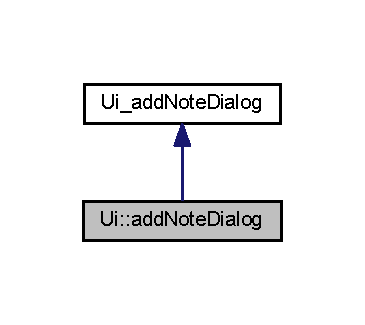
\includegraphics[width=175pt]{classUi_1_1addNoteDialog__inherit__graph}
\end{center}
\end{figure}


Collaboration diagram for Ui\+:\+:add\+Note\+Dialog\+:
\nopagebreak
\begin{figure}[H]
\begin{center}
\leavevmode
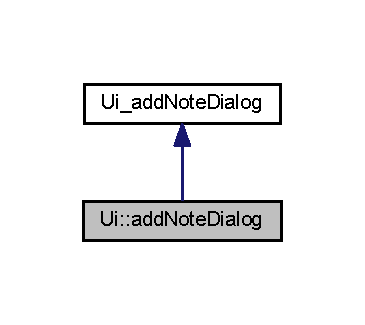
\includegraphics[width=175pt]{classUi_1_1addNoteDialog__coll__graph}
\end{center}
\end{figure}
\subsection*{Additional Inherited Members}


\subsection{Detailed Description}


Definition at line 173 of file ui\+\_\+add\+Note\+Dialog.\+h.



The documentation for this class was generated from the following file\+:\begin{DoxyCompactItemize}
\item 
C\+:/\+Users/\+Ogrigorieva/\+Visual Studio 2015/\+Projects/\+Personal/\+Matty\+Notes/\+Generated\+Files/\hyperlink{ui__addNoteDialog_8h}{ui\+\_\+add\+Note\+Dialog.\+h}\end{DoxyCompactItemize}

\hypertarget{classConstants}{}\section{Constants Class Reference}
\label{classConstants}\index{Constants@{Constants}}


{\ttfamily \#include $<$Constants.\+h$>$}

\subsection*{Public Member Functions}
\begin{DoxyCompactItemize}
\item 
\hyperlink{classConstants_af395b3c1d6f0577f4880a21a257aa1db}{Constants} ()
\item 
\hyperlink{classConstants_a2dce6c6db3f1ba4114550606fae1765a}{$\sim$\+Constants} ()
\end{DoxyCompactItemize}
\subsection*{Static Public Member Functions}
\begin{DoxyCompactItemize}
\item 
static void \hyperlink{classConstants_a3d474cb2c4e964cb64ab6f2db6e1bf92}{set\+Path\+To\+Db} (\hyperlink{Constants_8h_a9558e0854b1cdaf803f7a80df80ab91b}{Matty\+Path\+To\+Db\+Type} Path\+Type)
\item 
static void \hyperlink{classConstants_ab9a63f6d49de9a335b18e5ac543ec0fc}{set\+Path\+To\+Db} (Q\+String \&Path)
\end{DoxyCompactItemize}
\subsection*{Static Public Attributes}
\begin{DoxyCompactItemize}
\item 
static Q\+String \hyperlink{classConstants_a2a8fc008322275c6dfbc1f18a781c405}{Path\+To\+Db} = \char`\"{}\char`\"{}
\item 
static const Q\+String \hyperlink{classConstants_aa6a4e4e111634badc8b8aeba9df024ce}{Time\+Separator} = \char`\"{}\+:\char`\"{}
\item 
static const Q\+String \hyperlink{classConstants_a1b884c97c8f0c86fa5f8e050e38deca4}{Date\+Separator} = \char`\"{}.\char`\"{}
\item 
static const Q\+String \hyperlink{classConstants_a60b54ff297949426391e55991f80ccf2}{Empty\+Q\+String} = \char`\"{}\char`\"{}
\item 
static const Q\+String \hyperlink{classConstants_ade4aef58a5c7280c4f0bd40ba7b30f3c}{Space} = \char`\"{} \char`\"{}
\item 
static const Q\+String \hyperlink{classConstants_ace4bddf4b2dc0e05c8fec643238531a9}{Zero\+To\+Fill} = \char`\"{}0\char`\"{}
\item 
static const int \hyperlink{classConstants_a577e140cbb46e0fe143af8c18c29cee1}{Time\+Q\+String\+Length} = 5
\item 
static const int \hyperlink{classConstants_ae5b9b8df2388680fdacc61f9c247307d}{Date\+Q\+String\+Length} = 10
\item 
static const int \hyperlink{classConstants_aeade44a42999a2037171cc8b04031edb}{Position\+Of\+First\+Date\+Separator} = 2
\item 
static const int \hyperlink{classConstants_a6d9e83adc428b25381bc25b2e38843ea}{Position\+Of\+Second\+Date\+Separator} = 5
\end{DoxyCompactItemize}


\subsection{Detailed Description}


Definition at line 10 of file Constants.\+h.



\subsection{Constructor \& Destructor Documentation}
\hypertarget{classConstants_af395b3c1d6f0577f4880a21a257aa1db}{}\label{classConstants_af395b3c1d6f0577f4880a21a257aa1db} 
\index{Constants@{Constants}!Constants@{Constants}}
\index{Constants@{Constants}!Constants@{Constants}}
\subsubsection{\texorpdfstring{Constants()}{Constants()}}
{\footnotesize\ttfamily Constants\+::\+Constants (\begin{DoxyParamCaption}{ }\end{DoxyParamCaption})}



Definition at line 45 of file Constants.\+cpp.

\hypertarget{classConstants_a2dce6c6db3f1ba4114550606fae1765a}{}\label{classConstants_a2dce6c6db3f1ba4114550606fae1765a} 
\index{Constants@{Constants}!````~Constants@{$\sim$\+Constants}}
\index{````~Constants@{$\sim$\+Constants}!Constants@{Constants}}
\subsubsection{\texorpdfstring{$\sim$\+Constants()}{~Constants()}}
{\footnotesize\ttfamily Constants\+::$\sim$\+Constants (\begin{DoxyParamCaption}{ }\end{DoxyParamCaption})}



Definition at line 50 of file Constants.\+cpp.



\subsection{Member Function Documentation}
\hypertarget{classConstants_a3d474cb2c4e964cb64ab6f2db6e1bf92}{}\label{classConstants_a3d474cb2c4e964cb64ab6f2db6e1bf92} 
\index{Constants@{Constants}!set\+Path\+To\+Db@{set\+Path\+To\+Db}}
\index{set\+Path\+To\+Db@{set\+Path\+To\+Db}!Constants@{Constants}}
\subsubsection{\texorpdfstring{set\+Path\+To\+Db()}{setPathToDb()}\hspace{0.1cm}{\footnotesize\ttfamily [1/2]}}
{\footnotesize\ttfamily void Constants\+::set\+Path\+To\+Db (\begin{DoxyParamCaption}\item[{\hyperlink{Constants_8h_a9558e0854b1cdaf803f7a80df80ab91b}{Matty\+Path\+To\+Db\+Type}}]{Path\+Type }\end{DoxyParamCaption})\hspace{0.3cm}{\ttfamily [static]}}



Definition at line 21 of file Constants.\+cpp.

Here is the caller graph for this function\+:
% FIG 0
\hypertarget{classConstants_ab9a63f6d49de9a335b18e5ac543ec0fc}{}\label{classConstants_ab9a63f6d49de9a335b18e5ac543ec0fc} 
\index{Constants@{Constants}!set\+Path\+To\+Db@{set\+Path\+To\+Db}}
\index{set\+Path\+To\+Db@{set\+Path\+To\+Db}!Constants@{Constants}}
\subsubsection{\texorpdfstring{set\+Path\+To\+Db()}{setPathToDb()}\hspace{0.1cm}{\footnotesize\ttfamily [2/2]}}
{\footnotesize\ttfamily void Constants\+::set\+Path\+To\+Db (\begin{DoxyParamCaption}\item[{Q\+String \&}]{Path }\end{DoxyParamCaption})\hspace{0.3cm}{\ttfamily [static]}}



Definition at line 40 of file Constants.\+cpp.



\subsection{Member Data Documentation}
\hypertarget{classConstants_ae5b9b8df2388680fdacc61f9c247307d}{}\label{classConstants_ae5b9b8df2388680fdacc61f9c247307d} 
\index{Constants@{Constants}!Date\+Q\+String\+Length@{Date\+Q\+String\+Length}}
\index{Date\+Q\+String\+Length@{Date\+Q\+String\+Length}!Constants@{Constants}}
\subsubsection{\texorpdfstring{Date\+Q\+String\+Length}{DateQStringLength}}
{\footnotesize\ttfamily const int Constants\+::\+Date\+Q\+String\+Length = 10\hspace{0.3cm}{\ttfamily [static]}}



Definition at line 20 of file Constants.\+h.

\hypertarget{classConstants_a1b884c97c8f0c86fa5f8e050e38deca4}{}\label{classConstants_a1b884c97c8f0c86fa5f8e050e38deca4} 
\index{Constants@{Constants}!Date\+Separator@{Date\+Separator}}
\index{Date\+Separator@{Date\+Separator}!Constants@{Constants}}
\subsubsection{\texorpdfstring{Date\+Separator}{DateSeparator}}
{\footnotesize\ttfamily const Q\+String Constants\+::\+Date\+Separator = \char`\"{}.\char`\"{}\hspace{0.3cm}{\ttfamily [static]}}



Definition at line 15 of file Constants.\+h.

\hypertarget{classConstants_a60b54ff297949426391e55991f80ccf2}{}\label{classConstants_a60b54ff297949426391e55991f80ccf2} 
\index{Constants@{Constants}!Empty\+Q\+String@{Empty\+Q\+String}}
\index{Empty\+Q\+String@{Empty\+Q\+String}!Constants@{Constants}}
\subsubsection{\texorpdfstring{Empty\+Q\+String}{EmptyQString}}
{\footnotesize\ttfamily const Q\+String Constants\+::\+Empty\+Q\+String = \char`\"{}\char`\"{}\hspace{0.3cm}{\ttfamily [static]}}



Definition at line 16 of file Constants.\+h.

\hypertarget{classConstants_a2a8fc008322275c6dfbc1f18a781c405}{}\label{classConstants_a2a8fc008322275c6dfbc1f18a781c405} 
\index{Constants@{Constants}!Path\+To\+Db@{Path\+To\+Db}}
\index{Path\+To\+Db@{Path\+To\+Db}!Constants@{Constants}}
\subsubsection{\texorpdfstring{Path\+To\+Db}{PathToDb}}
{\footnotesize\ttfamily Q\+String Constants\+::\+Path\+To\+Db = \char`\"{}\char`\"{}\hspace{0.3cm}{\ttfamily [static]}}



Definition at line 13 of file Constants.\+h.

\hypertarget{classConstants_aeade44a42999a2037171cc8b04031edb}{}\label{classConstants_aeade44a42999a2037171cc8b04031edb} 
\index{Constants@{Constants}!Position\+Of\+First\+Date\+Separator@{Position\+Of\+First\+Date\+Separator}}
\index{Position\+Of\+First\+Date\+Separator@{Position\+Of\+First\+Date\+Separator}!Constants@{Constants}}
\subsubsection{\texorpdfstring{Position\+Of\+First\+Date\+Separator}{PositionOfFirstDateSeparator}}
{\footnotesize\ttfamily const int Constants\+::\+Position\+Of\+First\+Date\+Separator = 2\hspace{0.3cm}{\ttfamily [static]}}



Definition at line 21 of file Constants.\+h.

\hypertarget{classConstants_a6d9e83adc428b25381bc25b2e38843ea}{}\label{classConstants_a6d9e83adc428b25381bc25b2e38843ea} 
\index{Constants@{Constants}!Position\+Of\+Second\+Date\+Separator@{Position\+Of\+Second\+Date\+Separator}}
\index{Position\+Of\+Second\+Date\+Separator@{Position\+Of\+Second\+Date\+Separator}!Constants@{Constants}}
\subsubsection{\texorpdfstring{Position\+Of\+Second\+Date\+Separator}{PositionOfSecondDateSeparator}}
{\footnotesize\ttfamily const int Constants\+::\+Position\+Of\+Second\+Date\+Separator = 5\hspace{0.3cm}{\ttfamily [static]}}



Definition at line 22 of file Constants.\+h.

\hypertarget{classConstants_ade4aef58a5c7280c4f0bd40ba7b30f3c}{}\label{classConstants_ade4aef58a5c7280c4f0bd40ba7b30f3c} 
\index{Constants@{Constants}!Space@{Space}}
\index{Space@{Space}!Constants@{Constants}}
\subsubsection{\texorpdfstring{Space}{Space}}
{\footnotesize\ttfamily const Q\+String Constants\+::\+Space = \char`\"{} \char`\"{}\hspace{0.3cm}{\ttfamily [static]}}



Definition at line 17 of file Constants.\+h.

\hypertarget{classConstants_a577e140cbb46e0fe143af8c18c29cee1}{}\label{classConstants_a577e140cbb46e0fe143af8c18c29cee1} 
\index{Constants@{Constants}!Time\+Q\+String\+Length@{Time\+Q\+String\+Length}}
\index{Time\+Q\+String\+Length@{Time\+Q\+String\+Length}!Constants@{Constants}}
\subsubsection{\texorpdfstring{Time\+Q\+String\+Length}{TimeQStringLength}}
{\footnotesize\ttfamily const int Constants\+::\+Time\+Q\+String\+Length = 5\hspace{0.3cm}{\ttfamily [static]}}



Definition at line 19 of file Constants.\+h.

\hypertarget{classConstants_aa6a4e4e111634badc8b8aeba9df024ce}{}\label{classConstants_aa6a4e4e111634badc8b8aeba9df024ce} 
\index{Constants@{Constants}!Time\+Separator@{Time\+Separator}}
\index{Time\+Separator@{Time\+Separator}!Constants@{Constants}}
\subsubsection{\texorpdfstring{Time\+Separator}{TimeSeparator}}
{\footnotesize\ttfamily const Q\+String Constants\+::\+Time\+Separator = \char`\"{}\+:\char`\"{}\hspace{0.3cm}{\ttfamily [static]}}



Definition at line 14 of file Constants.\+h.

\hypertarget{classConstants_ace4bddf4b2dc0e05c8fec643238531a9}{}\label{classConstants_ace4bddf4b2dc0e05c8fec643238531a9} 
\index{Constants@{Constants}!Zero\+To\+Fill@{Zero\+To\+Fill}}
\index{Zero\+To\+Fill@{Zero\+To\+Fill}!Constants@{Constants}}
\subsubsection{\texorpdfstring{Zero\+To\+Fill}{ZeroToFill}}
{\footnotesize\ttfamily const Q\+String Constants\+::\+Zero\+To\+Fill = \char`\"{}0\char`\"{}\hspace{0.3cm}{\ttfamily [static]}}



Definition at line 18 of file Constants.\+h.



The documentation for this class was generated from the following files\+:\begin{DoxyCompactItemize}
\item 
C\+:/\+Users/\+Ogrigorieva/\+Visual Studio 2015/\+Projects/\+Personal/\+Matty\+Notes/\hyperlink{Constants_8h}{Constants.\+h}\item 
C\+:/\+Users/\+Ogrigorieva/\+Visual Studio 2015/\+Projects/\+Personal/\+Matty\+Notes/\hyperlink{Constants_8cpp}{Constants.\+cpp}\end{DoxyCompactItemize}

\hypertarget{classDbManager}{}\section{Db\+Manager Class Reference}
\label{classDbManager}\index{Db\+Manager@{Db\+Manager}}


{\ttfamily \#include $<$Db\+Manager.\+h$>$}

\subsection*{Public Member Functions}
\begin{DoxyCompactItemize}
\item 
\hyperlink{classDbManager_a0d16cf5bba931362e6c581eb1b5ba66a}{Db\+Manager} ()
\item 
\hyperlink{classDbManager_ac5cdf8e5e932d1681ab807d8f256374c}{$\sim$\+Db\+Manager} ()
\end{DoxyCompactItemize}
\subsection*{Static Public Member Functions}
\begin{DoxyCompactItemize}
\item 
static bool \hyperlink{classDbManager_abc90b3bf97dda268b4160a0662305898}{connect} (const Q\+String \&path)
\item 
static bool \hyperlink{classDbManager_a0d97afdec08f212ec39100d26d8b4273}{add\+Note} (\hyperlink{classMattyNote}{Matty\+Note} $\ast$Note)
\item 
static bool \hyperlink{classDbManager_a164849758fd05445c7af2cc04fc3569f}{delete\+Note} (int Note\+Id)
\item 
static void \hyperlink{classDbManager_a96908aac2c76d86fb1861ac8f755b962}{show\+Note} ()
\item 
static Q\+Sql\+Table\+Model $\ast$ \hyperlink{classDbManager_ac4e759380194e624382e267432de5357}{get\+Model} (const Q\+String \&path)
\item 
static Q\+String\+List \hyperlink{classDbManager_ade7585873652935bb12cb1ad546ceba2}{get\+Types} ()
\item 
static Q\+String \hyperlink{classDbManager_a6cb58e12049873e8b1b4b6ecd74dbfb6}{get\+Type\+Name} (int Type\+Id)
\item 
static int \hyperlink{classDbManager_a92ebefd0d5fae643db1fc51cc7ea0c31}{get\+Type\+Id} (const Q\+String \&Type\+Name)
\item 
static int \hyperlink{classDbManager_ae3998b50545d88a27d4361053f39b050}{get\+Note\+Count} ()
\item 
static Q\+Vector$<$ Q\+String\+List $>$ \hyperlink{classDbManager_a9b35a902ca6a35cd2589a3d1fffda94b}{get\+All\+Notes\+Order\+By\+Cr\+Date} ()
\end{DoxyCompactItemize}
\subsection*{Static Private Attributes}
\begin{DoxyCompactItemize}
\item 
static Q\+Sql\+Database \hyperlink{classDbManager_a3f6052f559a7a72eef66848ebc9f3eaa}{Matty\+Notes\+Db}
\end{DoxyCompactItemize}


\subsection{Detailed Description}


Definition at line 12 of file Db\+Manager.\+h.



\subsection{Constructor \& Destructor Documentation}
\hypertarget{classDbManager_a0d16cf5bba931362e6c581eb1b5ba66a}{}\label{classDbManager_a0d16cf5bba931362e6c581eb1b5ba66a} 
\index{Db\+Manager@{Db\+Manager}!Db\+Manager@{Db\+Manager}}
\index{Db\+Manager@{Db\+Manager}!Db\+Manager@{Db\+Manager}}
\subsubsection{\texorpdfstring{Db\+Manager()}{DbManager()}}
{\footnotesize\ttfamily Db\+Manager\+::\+Db\+Manager (\begin{DoxyParamCaption}{ }\end{DoxyParamCaption})}



Definition at line 11 of file Db\+Manager.\+cpp.

\hypertarget{classDbManager_ac5cdf8e5e932d1681ab807d8f256374c}{}\label{classDbManager_ac5cdf8e5e932d1681ab807d8f256374c} 
\index{Db\+Manager@{Db\+Manager}!````~Db\+Manager@{$\sim$\+Db\+Manager}}
\index{````~Db\+Manager@{$\sim$\+Db\+Manager}!Db\+Manager@{Db\+Manager}}
\subsubsection{\texorpdfstring{$\sim$\+Db\+Manager()}{~DbManager()}}
{\footnotesize\ttfamily Db\+Manager\+::$\sim$\+Db\+Manager (\begin{DoxyParamCaption}{ }\end{DoxyParamCaption})}



Definition at line 116 of file Db\+Manager.\+cpp.



\subsection{Member Function Documentation}
\hypertarget{classDbManager_a0d97afdec08f212ec39100d26d8b4273}{}\label{classDbManager_a0d97afdec08f212ec39100d26d8b4273} 
\index{Db\+Manager@{Db\+Manager}!add\+Note@{add\+Note}}
\index{add\+Note@{add\+Note}!Db\+Manager@{Db\+Manager}}
\subsubsection{\texorpdfstring{add\+Note()}{addNote()}}
{\footnotesize\ttfamily bool Db\+Manager\+::add\+Note (\begin{DoxyParamCaption}\item[{\hyperlink{classMattyNote}{Matty\+Note} $\ast$}]{Note }\end{DoxyParamCaption})\hspace{0.3cm}{\ttfamily [static]}}



Definition at line 16 of file Db\+Manager.\+cpp.

Here is the call graph for this function\+:
% FIG 0
Here is the caller graph for this function\+:
% FIG 1
\hypertarget{classDbManager_abc90b3bf97dda268b4160a0662305898}{}\label{classDbManager_abc90b3bf97dda268b4160a0662305898} 
\index{Db\+Manager@{Db\+Manager}!connect@{connect}}
\index{connect@{connect}!Db\+Manager@{Db\+Manager}}
\subsubsection{\texorpdfstring{connect()}{connect()}}
{\footnotesize\ttfamily bool Db\+Manager\+::connect (\begin{DoxyParamCaption}\item[{const Q\+String \&}]{path }\end{DoxyParamCaption})\hspace{0.3cm}{\ttfamily [static]}}



Definition at line 120 of file Db\+Manager.\+cpp.

Here is the caller graph for this function\+:
% FIG 2
\hypertarget{classDbManager_a164849758fd05445c7af2cc04fc3569f}{}\label{classDbManager_a164849758fd05445c7af2cc04fc3569f} 
\index{Db\+Manager@{Db\+Manager}!delete\+Note@{delete\+Note}}
\index{delete\+Note@{delete\+Note}!Db\+Manager@{Db\+Manager}}
\subsubsection{\texorpdfstring{delete\+Note()}{deleteNote()}}
{\footnotesize\ttfamily bool Db\+Manager\+::delete\+Note (\begin{DoxyParamCaption}\item[{int}]{Note\+Id }\end{DoxyParamCaption})\hspace{0.3cm}{\ttfamily [static]}}



Definition at line 33 of file Db\+Manager.\+cpp.

Here is the caller graph for this function\+:
% FIG 3
\hypertarget{classDbManager_a9b35a902ca6a35cd2589a3d1fffda94b}{}\label{classDbManager_a9b35a902ca6a35cd2589a3d1fffda94b} 
\index{Db\+Manager@{Db\+Manager}!get\+All\+Notes\+Order\+By\+Cr\+Date@{get\+All\+Notes\+Order\+By\+Cr\+Date}}
\index{get\+All\+Notes\+Order\+By\+Cr\+Date@{get\+All\+Notes\+Order\+By\+Cr\+Date}!Db\+Manager@{Db\+Manager}}
\subsubsection{\texorpdfstring{get\+All\+Notes\+Order\+By\+Cr\+Date()}{getAllNotesOrderByCrDate()}}
{\footnotesize\ttfamily Q\+Vector$<$ Q\+String\+List $>$ Db\+Manager\+::get\+All\+Notes\+Order\+By\+Cr\+Date (\begin{DoxyParamCaption}{ }\end{DoxyParamCaption})\hspace{0.3cm}{\ttfamily [static]}}



Definition at line 98 of file Db\+Manager.\+cpp.

Here is the caller graph for this function\+:
% FIG 4
\hypertarget{classDbManager_ac4e759380194e624382e267432de5357}{}\label{classDbManager_ac4e759380194e624382e267432de5357} 
\index{Db\+Manager@{Db\+Manager}!get\+Model@{get\+Model}}
\index{get\+Model@{get\+Model}!Db\+Manager@{Db\+Manager}}
\subsubsection{\texorpdfstring{get\+Model()}{getModel()}}
{\footnotesize\ttfamily Q\+Sql\+Table\+Model $\ast$ Db\+Manager\+::get\+Model (\begin{DoxyParamCaption}\item[{const Q\+String \&}]{path }\end{DoxyParamCaption})\hspace{0.3cm}{\ttfamily [static]}}



Definition at line 45 of file Db\+Manager.\+cpp.

\hypertarget{classDbManager_ae3998b50545d88a27d4361053f39b050}{}\label{classDbManager_ae3998b50545d88a27d4361053f39b050} 
\index{Db\+Manager@{Db\+Manager}!get\+Note\+Count@{get\+Note\+Count}}
\index{get\+Note\+Count@{get\+Note\+Count}!Db\+Manager@{Db\+Manager}}
\subsubsection{\texorpdfstring{get\+Note\+Count()}{getNoteCount()}}
{\footnotesize\ttfamily int Db\+Manager\+::get\+Note\+Count (\begin{DoxyParamCaption}{ }\end{DoxyParamCaption})\hspace{0.3cm}{\ttfamily [static]}}



Definition at line 88 of file Db\+Manager.\+cpp.

\hypertarget{classDbManager_a92ebefd0d5fae643db1fc51cc7ea0c31}{}\label{classDbManager_a92ebefd0d5fae643db1fc51cc7ea0c31} 
\index{Db\+Manager@{Db\+Manager}!get\+Type\+Id@{get\+Type\+Id}}
\index{get\+Type\+Id@{get\+Type\+Id}!Db\+Manager@{Db\+Manager}}
\subsubsection{\texorpdfstring{get\+Type\+Id()}{getTypeId()}}
{\footnotesize\ttfamily int Db\+Manager\+::get\+Type\+Id (\begin{DoxyParamCaption}\item[{const Q\+String \&}]{Type\+Name }\end{DoxyParamCaption})\hspace{0.3cm}{\ttfamily [static]}}



Definition at line 77 of file Db\+Manager.\+cpp.

Here is the caller graph for this function\+:
% FIG 5
\hypertarget{classDbManager_a6cb58e12049873e8b1b4b6ecd74dbfb6}{}\label{classDbManager_a6cb58e12049873e8b1b4b6ecd74dbfb6} 
\index{Db\+Manager@{Db\+Manager}!get\+Type\+Name@{get\+Type\+Name}}
\index{get\+Type\+Name@{get\+Type\+Name}!Db\+Manager@{Db\+Manager}}
\subsubsection{\texorpdfstring{get\+Type\+Name()}{getTypeName()}}
{\footnotesize\ttfamily Q\+String Db\+Manager\+::get\+Type\+Name (\begin{DoxyParamCaption}\item[{int}]{Type\+Id }\end{DoxyParamCaption})\hspace{0.3cm}{\ttfamily [static]}}



Definition at line 66 of file Db\+Manager.\+cpp.

Here is the caller graph for this function\+:
% FIG 6
\hypertarget{classDbManager_ade7585873652935bb12cb1ad546ceba2}{}\label{classDbManager_ade7585873652935bb12cb1ad546ceba2} 
\index{Db\+Manager@{Db\+Manager}!get\+Types@{get\+Types}}
\index{get\+Types@{get\+Types}!Db\+Manager@{Db\+Manager}}
\subsubsection{\texorpdfstring{get\+Types()}{getTypes()}}
{\footnotesize\ttfamily Q\+String\+List Db\+Manager\+::get\+Types (\begin{DoxyParamCaption}{ }\end{DoxyParamCaption})\hspace{0.3cm}{\ttfamily [static]}}



Definition at line 54 of file Db\+Manager.\+cpp.

Here is the caller graph for this function\+:
% FIG 7
\hypertarget{classDbManager_a96908aac2c76d86fb1861ac8f755b962}{}\label{classDbManager_a96908aac2c76d86fb1861ac8f755b962} 
\index{Db\+Manager@{Db\+Manager}!show\+Note@{show\+Note}}
\index{show\+Note@{show\+Note}!Db\+Manager@{Db\+Manager}}
\subsubsection{\texorpdfstring{show\+Note()}{showNote()}}
{\footnotesize\ttfamily void Db\+Manager\+::show\+Note (\begin{DoxyParamCaption}{ }\end{DoxyParamCaption})\hspace{0.3cm}{\ttfamily [static]}}



Definition at line 40 of file Db\+Manager.\+cpp.



\subsection{Member Data Documentation}
\hypertarget{classDbManager_a3f6052f559a7a72eef66848ebc9f3eaa}{}\label{classDbManager_a3f6052f559a7a72eef66848ebc9f3eaa} 
\index{Db\+Manager@{Db\+Manager}!Matty\+Notes\+Db@{Matty\+Notes\+Db}}
\index{Matty\+Notes\+Db@{Matty\+Notes\+Db}!Db\+Manager@{Db\+Manager}}
\subsubsection{\texorpdfstring{Matty\+Notes\+Db}{MattyNotesDb}}
{\footnotesize\ttfamily Q\+Sql\+Database Db\+Manager\+::\+Matty\+Notes\+Db\hspace{0.3cm}{\ttfamily [static]}, {\ttfamily [private]}}



Definition at line 28 of file Db\+Manager.\+h.



The documentation for this class was generated from the following files\+:\begin{DoxyCompactItemize}
\item 
C\+:/\+Users/\+Ogrigorieva/\+Visual Studio 2015/\+Projects/\+Personal/\+Matty\+Notes/\hyperlink{DbManager_8h}{Db\+Manager.\+h}\item 
C\+:/\+Users/\+Ogrigorieva/\+Visual Studio 2015/\+Projects/\+Personal/\+Matty\+Notes/\hyperlink{DbManager_8cpp}{Db\+Manager.\+cpp}\end{DoxyCompactItemize}

\hypertarget{classMattyGroupBox}{}\section{Matty\+Group\+Box Class Reference}
\label{classMattyGroupBox}\index{Matty\+Group\+Box@{Matty\+Group\+Box}}


{\ttfamily \#include $<$Matty\+Group\+Box.\+h$>$}



Inheritance diagram for Matty\+Group\+Box\+:
% FIG 0


Collaboration diagram for Matty\+Group\+Box\+:
% FIG 1
\subsection*{Public Member Functions}
\begin{DoxyCompactItemize}
\item 
\hyperlink{classMattyGroupBox_aa44b29a1b8b8f5129f52c2972c24aecd}{Matty\+Group\+Box} ()
\item 
void \hyperlink{classMattyGroupBox_a4cbc1800e9ec63cdd0e064d3a3738b80}{fill\+Frame} (class \hyperlink{classMattyNote}{Matty\+Note} \&This\+Note)
\item 
\hyperlink{classMattyGroupBox_acf5f5023cf210a83e9846a35b149dd70}{$\sim$\+Matty\+Group\+Box} ()
\end{DoxyCompactItemize}
\subsection*{Private Slots}
\begin{DoxyCompactItemize}
\item 
void \hyperlink{classMattyGroupBox_ac7b7f1db6ea96e4c4b0f58fb87f86900}{delete\+Note} ()
\end{DoxyCompactItemize}
\subsection*{Private Member Functions}
\begin{DoxyCompactItemize}
\item 
void \hyperlink{classMattyGroupBox_ae9862aae672bd2cf4a99da541beef696}{build\+Frame} ()
\end{DoxyCompactItemize}
\subsection*{Private Attributes}
\begin{DoxyCompactItemize}
\item 
Q\+Label $\ast$ \hyperlink{classMattyGroupBox_a7bd564ef71ea2331a316d2fc6792ef09}{Note\+Type\+Label}
\item 
Q\+Label $\ast$ \hyperlink{classMattyGroupBox_a1a71503d5ede703b934e4f02d932a038}{Note\+Cr\+Time\+And\+Date\+Label}
\item 
Q\+Label $\ast$ \hyperlink{classMattyGroupBox_a97b192413385021b01b34db7493f8b49}{Note\+Event\+Time\+And\+Date\+Label}
\item 
Q\+Label $\ast$ \hyperlink{classMattyGroupBox_a2243d04d95c060e516fa3a43f09f19ef}{Note\+Text\+Label}
\item 
Q\+Spacer\+Item $\ast$ \hyperlink{classMattyGroupBox_a6b2678b09a3c56c18f357775e83b76c0}{horizontal\+Spacer\+\_\+1}
\item 
Q\+Spacer\+Item $\ast$ \hyperlink{classMattyGroupBox_a633d989baf5de2db6d0c01702ba6b410}{horizontal\+Spacer\+\_\+2}
\item 
Q\+Spacer\+Item $\ast$ \hyperlink{classMattyGroupBox_ae622d8330b00272995af1d41ce037b4c}{vertical\+Spacer}
\item 
Q\+Push\+Button $\ast$ \hyperlink{classMattyGroupBox_a3237eef2287c1b2fcff14d226ef9116d}{edit\+Note\+Button}
\item 
Q\+Push\+Button $\ast$ \hyperlink{classMattyGroupBox_ab51a570cfe8b06f8ae06a7163fb09d4f}{delete\+Note\+Button}
\item 
Q\+H\+Box\+Layout $\ast$ \hyperlink{classMattyGroupBox_a5d52dd2e01ba1a5d155e056ea438f142}{horizontal\+Layout\+\_\+1}
\item 
Q\+H\+Box\+Layout $\ast$ \hyperlink{classMattyGroupBox_a053f7794bcd10214414d41e9c09663e0}{horizontal\+Layout\+\_\+2}
\item 
Q\+V\+Box\+Layout $\ast$ \hyperlink{classMattyGroupBox_a2fc280283ef68a61828fe26007c949f1}{vertical\+Layout}
\item 
Q\+Grid\+Layout $\ast$ \hyperlink{classMattyGroupBox_a02436c3690d2007eb0cba523bcb668ea}{grid\+Layout}
\item 
class \hyperlink{classMattyNote}{Matty\+Note} \hyperlink{classMattyGroupBox_a00ca2ef39a0b5aca9e83373777bed395}{This\+Group\+Box\+Note}
\end{DoxyCompactItemize}


\subsection{Detailed Description}


Definition at line 11 of file Matty\+Group\+Box.\+h.



\subsection{Constructor \& Destructor Documentation}
\hypertarget{classMattyGroupBox_aa44b29a1b8b8f5129f52c2972c24aecd}{}\label{classMattyGroupBox_aa44b29a1b8b8f5129f52c2972c24aecd} 
\index{Matty\+Group\+Box@{Matty\+Group\+Box}!Matty\+Group\+Box@{Matty\+Group\+Box}}
\index{Matty\+Group\+Box@{Matty\+Group\+Box}!Matty\+Group\+Box@{Matty\+Group\+Box}}
\subsubsection{\texorpdfstring{Matty\+Group\+Box()}{MattyGroupBox()}}
{\footnotesize\ttfamily Matty\+Group\+Box\+::\+Matty\+Group\+Box (\begin{DoxyParamCaption}{ }\end{DoxyParamCaption})}



Definition at line 8 of file Matty\+Group\+Box.\+cpp.

Here is the call graph for this function\+:
% FIG 2
\hypertarget{classMattyGroupBox_acf5f5023cf210a83e9846a35b149dd70}{}\label{classMattyGroupBox_acf5f5023cf210a83e9846a35b149dd70} 
\index{Matty\+Group\+Box@{Matty\+Group\+Box}!````~Matty\+Group\+Box@{$\sim$\+Matty\+Group\+Box}}
\index{````~Matty\+Group\+Box@{$\sim$\+Matty\+Group\+Box}!Matty\+Group\+Box@{Matty\+Group\+Box}}
\subsubsection{\texorpdfstring{$\sim$\+Matty\+Group\+Box()}{~MattyGroupBox()}}
{\footnotesize\ttfamily Matty\+Group\+Box\+::$\sim$\+Matty\+Group\+Box (\begin{DoxyParamCaption}{ }\end{DoxyParamCaption})}



Definition at line 193 of file Matty\+Group\+Box.\+cpp.

Here is the caller graph for this function\+:
% FIG 3


\subsection{Member Function Documentation}
\hypertarget{classMattyGroupBox_ae9862aae672bd2cf4a99da541beef696}{}\label{classMattyGroupBox_ae9862aae672bd2cf4a99da541beef696} 
\index{Matty\+Group\+Box@{Matty\+Group\+Box}!build\+Frame@{build\+Frame}}
\index{build\+Frame@{build\+Frame}!Matty\+Group\+Box@{Matty\+Group\+Box}}
\subsubsection{\texorpdfstring{build\+Frame()}{buildFrame()}}
{\footnotesize\ttfamily void Matty\+Group\+Box\+::build\+Frame (\begin{DoxyParamCaption}{ }\end{DoxyParamCaption})\hspace{0.3cm}{\ttfamily [private]}}



Definition at line 41 of file Matty\+Group\+Box.\+cpp.

Here is the caller graph for this function\+:
% FIG 4
\hypertarget{classMattyGroupBox_ac7b7f1db6ea96e4c4b0f58fb87f86900}{}\label{classMattyGroupBox_ac7b7f1db6ea96e4c4b0f58fb87f86900} 
\index{Matty\+Group\+Box@{Matty\+Group\+Box}!delete\+Note@{delete\+Note}}
\index{delete\+Note@{delete\+Note}!Matty\+Group\+Box@{Matty\+Group\+Box}}
\subsubsection{\texorpdfstring{delete\+Note}{deleteNote}}
{\footnotesize\ttfamily void Matty\+Group\+Box\+::delete\+Note (\begin{DoxyParamCaption}{ }\end{DoxyParamCaption})\hspace{0.3cm}{\ttfamily [private]}, {\ttfamily [slot]}}



Definition at line 163 of file Matty\+Group\+Box.\+cpp.

Here is the call graph for this function\+:
% FIG 5
Here is the caller graph for this function\+:
% FIG 6
\hypertarget{classMattyGroupBox_a4cbc1800e9ec63cdd0e064d3a3738b80}{}\label{classMattyGroupBox_a4cbc1800e9ec63cdd0e064d3a3738b80} 
\index{Matty\+Group\+Box@{Matty\+Group\+Box}!fill\+Frame@{fill\+Frame}}
\index{fill\+Frame@{fill\+Frame}!Matty\+Group\+Box@{Matty\+Group\+Box}}
\subsubsection{\texorpdfstring{fill\+Frame()}{fillFrame()}}
{\footnotesize\ttfamily void Matty\+Group\+Box\+::fill\+Frame (\begin{DoxyParamCaption}\item[{class \hyperlink{classMattyNote}{Matty\+Note} \&}]{This\+Note }\end{DoxyParamCaption})}



Definition at line 14 of file Matty\+Group\+Box.\+cpp.

Here is the call graph for this function\+:
% FIG 7
Here is the caller graph for this function\+:
% FIG 8


\subsection{Member Data Documentation}
\hypertarget{classMattyGroupBox_ab51a570cfe8b06f8ae06a7163fb09d4f}{}\label{classMattyGroupBox_ab51a570cfe8b06f8ae06a7163fb09d4f} 
\index{Matty\+Group\+Box@{Matty\+Group\+Box}!delete\+Note\+Button@{delete\+Note\+Button}}
\index{delete\+Note\+Button@{delete\+Note\+Button}!Matty\+Group\+Box@{Matty\+Group\+Box}}
\subsubsection{\texorpdfstring{delete\+Note\+Button}{deleteNoteButton}}
{\footnotesize\ttfamily Q\+Push\+Button$\ast$ Matty\+Group\+Box\+::delete\+Note\+Button\hspace{0.3cm}{\ttfamily [private]}}



Definition at line 30 of file Matty\+Group\+Box.\+h.

\hypertarget{classMattyGroupBox_a3237eef2287c1b2fcff14d226ef9116d}{}\label{classMattyGroupBox_a3237eef2287c1b2fcff14d226ef9116d} 
\index{Matty\+Group\+Box@{Matty\+Group\+Box}!edit\+Note\+Button@{edit\+Note\+Button}}
\index{edit\+Note\+Button@{edit\+Note\+Button}!Matty\+Group\+Box@{Matty\+Group\+Box}}
\subsubsection{\texorpdfstring{edit\+Note\+Button}{editNoteButton}}
{\footnotesize\ttfamily Q\+Push\+Button$\ast$ Matty\+Group\+Box\+::edit\+Note\+Button\hspace{0.3cm}{\ttfamily [private]}}



Definition at line 29 of file Matty\+Group\+Box.\+h.

\hypertarget{classMattyGroupBox_a02436c3690d2007eb0cba523bcb668ea}{}\label{classMattyGroupBox_a02436c3690d2007eb0cba523bcb668ea} 
\index{Matty\+Group\+Box@{Matty\+Group\+Box}!grid\+Layout@{grid\+Layout}}
\index{grid\+Layout@{grid\+Layout}!Matty\+Group\+Box@{Matty\+Group\+Box}}
\subsubsection{\texorpdfstring{grid\+Layout}{gridLayout}}
{\footnotesize\ttfamily Q\+Grid\+Layout$\ast$ Matty\+Group\+Box\+::grid\+Layout\hspace{0.3cm}{\ttfamily [private]}}



Definition at line 34 of file Matty\+Group\+Box.\+h.

\hypertarget{classMattyGroupBox_a5d52dd2e01ba1a5d155e056ea438f142}{}\label{classMattyGroupBox_a5d52dd2e01ba1a5d155e056ea438f142} 
\index{Matty\+Group\+Box@{Matty\+Group\+Box}!horizontal\+Layout\+\_\+1@{horizontal\+Layout\+\_\+1}}
\index{horizontal\+Layout\+\_\+1@{horizontal\+Layout\+\_\+1}!Matty\+Group\+Box@{Matty\+Group\+Box}}
\subsubsection{\texorpdfstring{horizontal\+Layout\+\_\+1}{horizontalLayout\_1}}
{\footnotesize\ttfamily Q\+H\+Box\+Layout$\ast$ Matty\+Group\+Box\+::horizontal\+Layout\+\_\+1\hspace{0.3cm}{\ttfamily [private]}}



Definition at line 31 of file Matty\+Group\+Box.\+h.

\hypertarget{classMattyGroupBox_a053f7794bcd10214414d41e9c09663e0}{}\label{classMattyGroupBox_a053f7794bcd10214414d41e9c09663e0} 
\index{Matty\+Group\+Box@{Matty\+Group\+Box}!horizontal\+Layout\+\_\+2@{horizontal\+Layout\+\_\+2}}
\index{horizontal\+Layout\+\_\+2@{horizontal\+Layout\+\_\+2}!Matty\+Group\+Box@{Matty\+Group\+Box}}
\subsubsection{\texorpdfstring{horizontal\+Layout\+\_\+2}{horizontalLayout\_2}}
{\footnotesize\ttfamily Q\+H\+Box\+Layout$\ast$ Matty\+Group\+Box\+::horizontal\+Layout\+\_\+2\hspace{0.3cm}{\ttfamily [private]}}



Definition at line 32 of file Matty\+Group\+Box.\+h.

\hypertarget{classMattyGroupBox_a6b2678b09a3c56c18f357775e83b76c0}{}\label{classMattyGroupBox_a6b2678b09a3c56c18f357775e83b76c0} 
\index{Matty\+Group\+Box@{Matty\+Group\+Box}!horizontal\+Spacer\+\_\+1@{horizontal\+Spacer\+\_\+1}}
\index{horizontal\+Spacer\+\_\+1@{horizontal\+Spacer\+\_\+1}!Matty\+Group\+Box@{Matty\+Group\+Box}}
\subsubsection{\texorpdfstring{horizontal\+Spacer\+\_\+1}{horizontalSpacer\_1}}
{\footnotesize\ttfamily Q\+Spacer\+Item$\ast$ Matty\+Group\+Box\+::horizontal\+Spacer\+\_\+1\hspace{0.3cm}{\ttfamily [private]}}



Definition at line 26 of file Matty\+Group\+Box.\+h.

\hypertarget{classMattyGroupBox_a633d989baf5de2db6d0c01702ba6b410}{}\label{classMattyGroupBox_a633d989baf5de2db6d0c01702ba6b410} 
\index{Matty\+Group\+Box@{Matty\+Group\+Box}!horizontal\+Spacer\+\_\+2@{horizontal\+Spacer\+\_\+2}}
\index{horizontal\+Spacer\+\_\+2@{horizontal\+Spacer\+\_\+2}!Matty\+Group\+Box@{Matty\+Group\+Box}}
\subsubsection{\texorpdfstring{horizontal\+Spacer\+\_\+2}{horizontalSpacer\_2}}
{\footnotesize\ttfamily Q\+Spacer\+Item$\ast$ Matty\+Group\+Box\+::horizontal\+Spacer\+\_\+2\hspace{0.3cm}{\ttfamily [private]}}



Definition at line 27 of file Matty\+Group\+Box.\+h.

\hypertarget{classMattyGroupBox_a1a71503d5ede703b934e4f02d932a038}{}\label{classMattyGroupBox_a1a71503d5ede703b934e4f02d932a038} 
\index{Matty\+Group\+Box@{Matty\+Group\+Box}!Note\+Cr\+Time\+And\+Date\+Label@{Note\+Cr\+Time\+And\+Date\+Label}}
\index{Note\+Cr\+Time\+And\+Date\+Label@{Note\+Cr\+Time\+And\+Date\+Label}!Matty\+Group\+Box@{Matty\+Group\+Box}}
\subsubsection{\texorpdfstring{Note\+Cr\+Time\+And\+Date\+Label}{NoteCrTimeAndDateLabel}}
{\footnotesize\ttfamily Q\+Label$\ast$ Matty\+Group\+Box\+::\+Note\+Cr\+Time\+And\+Date\+Label\hspace{0.3cm}{\ttfamily [private]}}



Definition at line 23 of file Matty\+Group\+Box.\+h.

\hypertarget{classMattyGroupBox_a97b192413385021b01b34db7493f8b49}{}\label{classMattyGroupBox_a97b192413385021b01b34db7493f8b49} 
\index{Matty\+Group\+Box@{Matty\+Group\+Box}!Note\+Event\+Time\+And\+Date\+Label@{Note\+Event\+Time\+And\+Date\+Label}}
\index{Note\+Event\+Time\+And\+Date\+Label@{Note\+Event\+Time\+And\+Date\+Label}!Matty\+Group\+Box@{Matty\+Group\+Box}}
\subsubsection{\texorpdfstring{Note\+Event\+Time\+And\+Date\+Label}{NoteEventTimeAndDateLabel}}
{\footnotesize\ttfamily Q\+Label$\ast$ Matty\+Group\+Box\+::\+Note\+Event\+Time\+And\+Date\+Label\hspace{0.3cm}{\ttfamily [private]}}



Definition at line 24 of file Matty\+Group\+Box.\+h.

\hypertarget{classMattyGroupBox_a2243d04d95c060e516fa3a43f09f19ef}{}\label{classMattyGroupBox_a2243d04d95c060e516fa3a43f09f19ef} 
\index{Matty\+Group\+Box@{Matty\+Group\+Box}!Note\+Text\+Label@{Note\+Text\+Label}}
\index{Note\+Text\+Label@{Note\+Text\+Label}!Matty\+Group\+Box@{Matty\+Group\+Box}}
\subsubsection{\texorpdfstring{Note\+Text\+Label}{NoteTextLabel}}
{\footnotesize\ttfamily Q\+Label$\ast$ Matty\+Group\+Box\+::\+Note\+Text\+Label\hspace{0.3cm}{\ttfamily [private]}}



Definition at line 25 of file Matty\+Group\+Box.\+h.

\hypertarget{classMattyGroupBox_a7bd564ef71ea2331a316d2fc6792ef09}{}\label{classMattyGroupBox_a7bd564ef71ea2331a316d2fc6792ef09} 
\index{Matty\+Group\+Box@{Matty\+Group\+Box}!Note\+Type\+Label@{Note\+Type\+Label}}
\index{Note\+Type\+Label@{Note\+Type\+Label}!Matty\+Group\+Box@{Matty\+Group\+Box}}
\subsubsection{\texorpdfstring{Note\+Type\+Label}{NoteTypeLabel}}
{\footnotesize\ttfamily Q\+Label$\ast$ Matty\+Group\+Box\+::\+Note\+Type\+Label\hspace{0.3cm}{\ttfamily [private]}}



Definition at line 22 of file Matty\+Group\+Box.\+h.

\hypertarget{classMattyGroupBox_a00ca2ef39a0b5aca9e83373777bed395}{}\label{classMattyGroupBox_a00ca2ef39a0b5aca9e83373777bed395} 
\index{Matty\+Group\+Box@{Matty\+Group\+Box}!This\+Group\+Box\+Note@{This\+Group\+Box\+Note}}
\index{This\+Group\+Box\+Note@{This\+Group\+Box\+Note}!Matty\+Group\+Box@{Matty\+Group\+Box}}
\subsubsection{\texorpdfstring{This\+Group\+Box\+Note}{ThisGroupBoxNote}}
{\footnotesize\ttfamily class \hyperlink{classMattyNote}{Matty\+Note} Matty\+Group\+Box\+::\+This\+Group\+Box\+Note\hspace{0.3cm}{\ttfamily [private]}}



Definition at line 35 of file Matty\+Group\+Box.\+h.

\hypertarget{classMattyGroupBox_a2fc280283ef68a61828fe26007c949f1}{}\label{classMattyGroupBox_a2fc280283ef68a61828fe26007c949f1} 
\index{Matty\+Group\+Box@{Matty\+Group\+Box}!vertical\+Layout@{vertical\+Layout}}
\index{vertical\+Layout@{vertical\+Layout}!Matty\+Group\+Box@{Matty\+Group\+Box}}
\subsubsection{\texorpdfstring{vertical\+Layout}{verticalLayout}}
{\footnotesize\ttfamily Q\+V\+Box\+Layout$\ast$ Matty\+Group\+Box\+::vertical\+Layout\hspace{0.3cm}{\ttfamily [private]}}



Definition at line 33 of file Matty\+Group\+Box.\+h.

\hypertarget{classMattyGroupBox_ae622d8330b00272995af1d41ce037b4c}{}\label{classMattyGroupBox_ae622d8330b00272995af1d41ce037b4c} 
\index{Matty\+Group\+Box@{Matty\+Group\+Box}!vertical\+Spacer@{vertical\+Spacer}}
\index{vertical\+Spacer@{vertical\+Spacer}!Matty\+Group\+Box@{Matty\+Group\+Box}}
\subsubsection{\texorpdfstring{vertical\+Spacer}{verticalSpacer}}
{\footnotesize\ttfamily Q\+Spacer\+Item$\ast$ Matty\+Group\+Box\+::vertical\+Spacer\hspace{0.3cm}{\ttfamily [private]}}



Definition at line 28 of file Matty\+Group\+Box.\+h.



The documentation for this class was generated from the following files\+:\begin{DoxyCompactItemize}
\item 
C\+:/\+Users/\+Ogrigorieva/\+Visual Studio 2015/\+Projects/\+Personal/\+Matty\+Notes/\hyperlink{MattyGroupBox_8h}{Matty\+Group\+Box.\+h}\item 
C\+:/\+Users/\+Ogrigorieva/\+Visual Studio 2015/\+Projects/\+Personal/\+Matty\+Notes/\hyperlink{MattyGroupBox_8cpp}{Matty\+Group\+Box.\+cpp}\end{DoxyCompactItemize}

\hypertarget{classMattyNote}{}\section{Matty\+Note Class Reference}
\label{classMattyNote}\index{Matty\+Note@{Matty\+Note}}


{\ttfamily \#include $<$Matty\+Note.\+h$>$}



Collaboration diagram for Matty\+Note\+:
% FIG 0
\subsection*{Public Member Functions}
\begin{DoxyCompactItemize}
\item 
\hyperlink{classMattyNote_a8c09bf366e6973bc1c4f4d5daa792899}{Matty\+Note} ()
\item 
\hyperlink{classMattyNote_a101e9c2475ee2567dfa2e168b543806f}{Matty\+Note} (Q\+String\+List Row\+From\+Db)
\item 
\hyperlink{classMattyNote_a2831641523b4a0d5c36100689f95c912}{$\sim$\+Matty\+Note} ()
\item 
void \hyperlink{classMattyNote_af7909f64608b020b501019cf29796eb0}{set\+Title} (const Q\+String \&Title)
\item 
void \hyperlink{classMattyNote_ac9171fd4faaf0c286c9315a0b4ef4560}{set\+Type} (const Q\+String \&Type\+Name)
\item 
void \hyperlink{classMattyNote_a8ae86d728b9cb64fa78042a09cb5aa70}{set\+Type} (int Type\+Id)
\item 
void \hyperlink{classMattyNote_afa0c4ee32401e4a09e8d04fd0b01da0b}{set\+Text} (const Q\+String \&Text)
\item 
void \hyperlink{classMattyNote_aaeba8670420ab9ad0fb8be660845e0ba}{set\+Event\+Time} (const Q\+String \&Event\+Time)
\item 
void \hyperlink{classMattyNote_a70676b1ab215b873c9451a82cc417684}{set\+Event\+Date} (const Q\+String \&Event\+Date)
\item 
Q\+String \hyperlink{classMattyNote_acb4af77f4177a0b17f140d4b4421e32e}{get\+Title} ()
\item 
Q\+String \hyperlink{classMattyNote_ad07b65692d79cf25e5c9008e111bd999}{get\+Type} ()
\item 
int \hyperlink{classMattyNote_af5b90028a8e406e41b8c8a6de83685ef}{get\+Type\+Id} ()
\item 
Q\+String \hyperlink{classMattyNote_a9213ac15a09625f59a95ede1b1470308}{get\+Text} ()
\item 
Q\+String \hyperlink{classMattyNote_a8c7f06ff44ce23f5a9ce6d2364732a24}{get\+Event\+Time} ()
\item 
Q\+String \hyperlink{classMattyNote_a8973578029ab29593061cca235ae84f9}{get\+Event\+Date} ()
\item 
Q\+String \hyperlink{classMattyNote_ac6f675c525f027536fdcfda43f0a261e}{get\+Ev\+Dayof\+Week} ()
\item 
Q\+String \hyperlink{classMattyNote_a2acf19aded7d4b5c29db7af6b0c4b1f6}{get\+Cr\+Time} ()
\item 
Q\+String \hyperlink{classMattyNote_ade5ef053d6d9ba158d9842feadd39754}{get\+Cr\+Date} ()
\item 
Q\+String \hyperlink{classMattyNote_a92dca9930c5f9b00991a780fc89acb8f}{get\+Cr\+Day\+Of\+Week} ()
\item 
int \hyperlink{classMattyNote_ad7c5837f61e4813005ae063c67b9a0f0}{get\+Note\+Id} ()
\item 
\hyperlink{structTimeAndDate}{Time\+And\+Date} \hyperlink{classMattyNote_ac2579a4c26f27c8d86b6a57c81f5dc3b}{get\+Event\+Time\+And\+Date} ()
\item 
\hyperlink{structTimeAndDate}{Time\+And\+Date} \hyperlink{classMattyNote_aff50eb125d7a0a64ac3fb21f056ec745}{get\+Cr\+Time\+And\+Date} ()
\end{DoxyCompactItemize}
\subsection*{Private Attributes}
\begin{DoxyCompactItemize}
\item 
int \hyperlink{classMattyNote_a15a3c21ef00e8c629aeb58025121b0a9}{Note\+Id}
\item 
int \hyperlink{classMattyNote_ad116cdf301951c8c93ee2a81a0df8647}{Note\+Type\+Id}
\item 
Q\+String \hyperlink{classMattyNote_a185f1f13eeb93acb237b9db7b4c94229}{Note\+Title}
\item 
Q\+String \hyperlink{classMattyNote_a0b45b382884fac5b651ab1ce155a2c13}{Note\+Type}
\item 
Q\+String \hyperlink{classMattyNote_ab54fa825ed3ce8081befdb0c391d682b}{Note\+Text}
\item 
Q\+String \hyperlink{classMattyNote_a3e69ae7fb7c8c616594a9647c14a192e}{Note\+Event\+Time}
\item 
Q\+String \hyperlink{classMattyNote_a9644cd6552e27c1875d83edce2469db3}{Note\+Event\+Date}
\item 
Q\+String \hyperlink{classMattyNote_a1182beac3edac3a7a7e4cdce72fc02ce}{Note\+Ev\+Day\+Of\+Week}
\item 
Q\+String \hyperlink{classMattyNote_a03208145949dfb98a99cfd9d95373418}{Note\+Cr\+Time}
\item 
Q\+String \hyperlink{classMattyNote_a3b94a4b062d2c2335f410f252210ed20}{Note\+Cr\+Date}
\item 
Q\+String \hyperlink{classMattyNote_a3776d088e67ef0181116b1cc2db3fd94}{Note\+Cr\+Day\+Of\+Week}
\item 
\hyperlink{classMattyTime}{Matty\+Time} \hyperlink{classMattyNote_a1f870bad84b62162b8ee07bff70e3003}{Event\+Time\+And\+Date}
\item 
\hyperlink{classMattyTime}{Matty\+Time} \hyperlink{classMattyNote_ae2959e86661be06281c70a5b87390587}{Cr\+Time\+And\+Date}
\end{DoxyCompactItemize}


\subsection{Detailed Description}


Definition at line 11 of file Matty\+Note.\+h.



\subsection{Constructor \& Destructor Documentation}
\hypertarget{classMattyNote_a8c09bf366e6973bc1c4f4d5daa792899}{}\label{classMattyNote_a8c09bf366e6973bc1c4f4d5daa792899} 
\index{Matty\+Note@{Matty\+Note}!Matty\+Note@{Matty\+Note}}
\index{Matty\+Note@{Matty\+Note}!Matty\+Note@{Matty\+Note}}
\subsubsection{\texorpdfstring{Matty\+Note()}{MattyNote()}\hspace{0.1cm}{\footnotesize\ttfamily [1/2]}}
{\footnotesize\ttfamily Matty\+Note\+::\+Matty\+Note (\begin{DoxyParamCaption}{ }\end{DoxyParamCaption})}



Definition at line 6 of file Matty\+Note.\+cpp.

Here is the call graph for this function\+:
% FIG 1
\hypertarget{classMattyNote_a101e9c2475ee2567dfa2e168b543806f}{}\label{classMattyNote_a101e9c2475ee2567dfa2e168b543806f} 
\index{Matty\+Note@{Matty\+Note}!Matty\+Note@{Matty\+Note}}
\index{Matty\+Note@{Matty\+Note}!Matty\+Note@{Matty\+Note}}
\subsubsection{\texorpdfstring{Matty\+Note()}{MattyNote()}\hspace{0.1cm}{\footnotesize\ttfamily [2/2]}}
{\footnotesize\ttfamily Matty\+Note\+::\+Matty\+Note (\begin{DoxyParamCaption}\item[{Q\+String\+List}]{Row\+From\+Db }\end{DoxyParamCaption})}



Definition at line 15 of file Matty\+Note.\+cpp.

Here is the call graph for this function\+:
% FIG 2
\hypertarget{classMattyNote_a2831641523b4a0d5c36100689f95c912}{}\label{classMattyNote_a2831641523b4a0d5c36100689f95c912} 
\index{Matty\+Note@{Matty\+Note}!````~Matty\+Note@{$\sim$\+Matty\+Note}}
\index{````~Matty\+Note@{$\sim$\+Matty\+Note}!Matty\+Note@{Matty\+Note}}
\subsubsection{\texorpdfstring{$\sim$\+Matty\+Note()}{~MattyNote()}}
{\footnotesize\ttfamily Matty\+Note\+::$\sim$\+Matty\+Note (\begin{DoxyParamCaption}{ }\end{DoxyParamCaption})}



Definition at line 29 of file Matty\+Note.\+cpp.



\subsection{Member Function Documentation}
\hypertarget{classMattyNote_ade5ef053d6d9ba158d9842feadd39754}{}\label{classMattyNote_ade5ef053d6d9ba158d9842feadd39754} 
\index{Matty\+Note@{Matty\+Note}!get\+Cr\+Date@{get\+Cr\+Date}}
\index{get\+Cr\+Date@{get\+Cr\+Date}!Matty\+Note@{Matty\+Note}}
\subsubsection{\texorpdfstring{get\+Cr\+Date()}{getCrDate()}}
{\footnotesize\ttfamily Q\+String Matty\+Note\+::get\+Cr\+Date (\begin{DoxyParamCaption}{ }\end{DoxyParamCaption})}



Definition at line 123 of file Matty\+Note.\+cpp.

Here is the caller graph for this function\+:
% FIG 3
\hypertarget{classMattyNote_a92dca9930c5f9b00991a780fc89acb8f}{}\label{classMattyNote_a92dca9930c5f9b00991a780fc89acb8f} 
\index{Matty\+Note@{Matty\+Note}!get\+Cr\+Day\+Of\+Week@{get\+Cr\+Day\+Of\+Week}}
\index{get\+Cr\+Day\+Of\+Week@{get\+Cr\+Day\+Of\+Week}!Matty\+Note@{Matty\+Note}}
\subsubsection{\texorpdfstring{get\+Cr\+Day\+Of\+Week()}{getCrDayOfWeek()}}
{\footnotesize\ttfamily Q\+String Matty\+Note\+::get\+Cr\+Day\+Of\+Week (\begin{DoxyParamCaption}{ }\end{DoxyParamCaption})}



Definition at line 128 of file Matty\+Note.\+cpp.

\hypertarget{classMattyNote_a2acf19aded7d4b5c29db7af6b0c4b1f6}{}\label{classMattyNote_a2acf19aded7d4b5c29db7af6b0c4b1f6} 
\index{Matty\+Note@{Matty\+Note}!get\+Cr\+Time@{get\+Cr\+Time}}
\index{get\+Cr\+Time@{get\+Cr\+Time}!Matty\+Note@{Matty\+Note}}
\subsubsection{\texorpdfstring{get\+Cr\+Time()}{getCrTime()}}
{\footnotesize\ttfamily Q\+String Matty\+Note\+::get\+Cr\+Time (\begin{DoxyParamCaption}{ }\end{DoxyParamCaption})}



Definition at line 118 of file Matty\+Note.\+cpp.

Here is the caller graph for this function\+:
% FIG 4
\hypertarget{classMattyNote_aff50eb125d7a0a64ac3fb21f056ec745}{}\label{classMattyNote_aff50eb125d7a0a64ac3fb21f056ec745} 
\index{Matty\+Note@{Matty\+Note}!get\+Cr\+Time\+And\+Date@{get\+Cr\+Time\+And\+Date}}
\index{get\+Cr\+Time\+And\+Date@{get\+Cr\+Time\+And\+Date}!Matty\+Note@{Matty\+Note}}
\subsubsection{\texorpdfstring{get\+Cr\+Time\+And\+Date()}{getCrTimeAndDate()}}
{\footnotesize\ttfamily \hyperlink{structTimeAndDate}{Time\+And\+Date} Matty\+Note\+::get\+Cr\+Time\+And\+Date (\begin{DoxyParamCaption}{ }\end{DoxyParamCaption})}



Definition at line 143 of file Matty\+Note.\+cpp.

\hypertarget{classMattyNote_ac6f675c525f027536fdcfda43f0a261e}{}\label{classMattyNote_ac6f675c525f027536fdcfda43f0a261e} 
\index{Matty\+Note@{Matty\+Note}!get\+Ev\+Dayof\+Week@{get\+Ev\+Dayof\+Week}}
\index{get\+Ev\+Dayof\+Week@{get\+Ev\+Dayof\+Week}!Matty\+Note@{Matty\+Note}}
\subsubsection{\texorpdfstring{get\+Ev\+Dayof\+Week()}{getEvDayofWeek()}}
{\footnotesize\ttfamily Q\+String Matty\+Note\+::get\+Ev\+Dayof\+Week (\begin{DoxyParamCaption}{ }\end{DoxyParamCaption})}



Definition at line 113 of file Matty\+Note.\+cpp.

Here is the caller graph for this function\+:
% FIG 5
\hypertarget{classMattyNote_a8973578029ab29593061cca235ae84f9}{}\label{classMattyNote_a8973578029ab29593061cca235ae84f9} 
\index{Matty\+Note@{Matty\+Note}!get\+Event\+Date@{get\+Event\+Date}}
\index{get\+Event\+Date@{get\+Event\+Date}!Matty\+Note@{Matty\+Note}}
\subsubsection{\texorpdfstring{get\+Event\+Date()}{getEventDate()}}
{\footnotesize\ttfamily Q\+String Matty\+Note\+::get\+Event\+Date (\begin{DoxyParamCaption}{ }\end{DoxyParamCaption})}



Definition at line 108 of file Matty\+Note.\+cpp.

Here is the caller graph for this function\+:
% FIG 6
\hypertarget{classMattyNote_a8c7f06ff44ce23f5a9ce6d2364732a24}{}\label{classMattyNote_a8c7f06ff44ce23f5a9ce6d2364732a24} 
\index{Matty\+Note@{Matty\+Note}!get\+Event\+Time@{get\+Event\+Time}}
\index{get\+Event\+Time@{get\+Event\+Time}!Matty\+Note@{Matty\+Note}}
\subsubsection{\texorpdfstring{get\+Event\+Time()}{getEventTime()}}
{\footnotesize\ttfamily Q\+String Matty\+Note\+::get\+Event\+Time (\begin{DoxyParamCaption}{ }\end{DoxyParamCaption})}



Definition at line 103 of file Matty\+Note.\+cpp.

Here is the caller graph for this function\+:
% FIG 7
\hypertarget{classMattyNote_ac2579a4c26f27c8d86b6a57c81f5dc3b}{}\label{classMattyNote_ac2579a4c26f27c8d86b6a57c81f5dc3b} 
\index{Matty\+Note@{Matty\+Note}!get\+Event\+Time\+And\+Date@{get\+Event\+Time\+And\+Date}}
\index{get\+Event\+Time\+And\+Date@{get\+Event\+Time\+And\+Date}!Matty\+Note@{Matty\+Note}}
\subsubsection{\texorpdfstring{get\+Event\+Time\+And\+Date()}{getEventTimeAndDate()}}
{\footnotesize\ttfamily \hyperlink{structTimeAndDate}{Time\+And\+Date} Matty\+Note\+::get\+Event\+Time\+And\+Date (\begin{DoxyParamCaption}{ }\end{DoxyParamCaption})}



Definition at line 138 of file Matty\+Note.\+cpp.

\hypertarget{classMattyNote_ad7c5837f61e4813005ae063c67b9a0f0}{}\label{classMattyNote_ad7c5837f61e4813005ae063c67b9a0f0} 
\index{Matty\+Note@{Matty\+Note}!get\+Note\+Id@{get\+Note\+Id}}
\index{get\+Note\+Id@{get\+Note\+Id}!Matty\+Note@{Matty\+Note}}
\subsubsection{\texorpdfstring{get\+Note\+Id()}{getNoteId()}}
{\footnotesize\ttfamily int Matty\+Note\+::get\+Note\+Id (\begin{DoxyParamCaption}{ }\end{DoxyParamCaption})}



Definition at line 133 of file Matty\+Note.\+cpp.

Here is the caller graph for this function\+:
% FIG 8
\hypertarget{classMattyNote_a9213ac15a09625f59a95ede1b1470308}{}\label{classMattyNote_a9213ac15a09625f59a95ede1b1470308} 
\index{Matty\+Note@{Matty\+Note}!get\+Text@{get\+Text}}
\index{get\+Text@{get\+Text}!Matty\+Note@{Matty\+Note}}
\subsubsection{\texorpdfstring{get\+Text()}{getText()}}
{\footnotesize\ttfamily Q\+String Matty\+Note\+::get\+Text (\begin{DoxyParamCaption}{ }\end{DoxyParamCaption})}



Definition at line 98 of file Matty\+Note.\+cpp.

Here is the caller graph for this function\+:
% FIG 9
\hypertarget{classMattyNote_acb4af77f4177a0b17f140d4b4421e32e}{}\label{classMattyNote_acb4af77f4177a0b17f140d4b4421e32e} 
\index{Matty\+Note@{Matty\+Note}!get\+Title@{get\+Title}}
\index{get\+Title@{get\+Title}!Matty\+Note@{Matty\+Note}}
\subsubsection{\texorpdfstring{get\+Title()}{getTitle()}}
{\footnotesize\ttfamily Q\+String Matty\+Note\+::get\+Title (\begin{DoxyParamCaption}{ }\end{DoxyParamCaption})}



Definition at line 83 of file Matty\+Note.\+cpp.

Here is the caller graph for this function\+:
% FIG 10
\hypertarget{classMattyNote_ad07b65692d79cf25e5c9008e111bd999}{}\label{classMattyNote_ad07b65692d79cf25e5c9008e111bd999} 
\index{Matty\+Note@{Matty\+Note}!get\+Type@{get\+Type}}
\index{get\+Type@{get\+Type}!Matty\+Note@{Matty\+Note}}
\subsubsection{\texorpdfstring{get\+Type()}{getType()}}
{\footnotesize\ttfamily Q\+String Matty\+Note\+::get\+Type (\begin{DoxyParamCaption}{ }\end{DoxyParamCaption})}



Definition at line 88 of file Matty\+Note.\+cpp.

Here is the caller graph for this function\+:
% FIG 11
\hypertarget{classMattyNote_af5b90028a8e406e41b8c8a6de83685ef}{}\label{classMattyNote_af5b90028a8e406e41b8c8a6de83685ef} 
\index{Matty\+Note@{Matty\+Note}!get\+Type\+Id@{get\+Type\+Id}}
\index{get\+Type\+Id@{get\+Type\+Id}!Matty\+Note@{Matty\+Note}}
\subsubsection{\texorpdfstring{get\+Type\+Id()}{getTypeId()}}
{\footnotesize\ttfamily int Matty\+Note\+::get\+Type\+Id (\begin{DoxyParamCaption}{ }\end{DoxyParamCaption})}



Definition at line 93 of file Matty\+Note.\+cpp.

Here is the caller graph for this function\+:
% FIG 12
\hypertarget{classMattyNote_a70676b1ab215b873c9451a82cc417684}{}\label{classMattyNote_a70676b1ab215b873c9451a82cc417684} 
\index{Matty\+Note@{Matty\+Note}!set\+Event\+Date@{set\+Event\+Date}}
\index{set\+Event\+Date@{set\+Event\+Date}!Matty\+Note@{Matty\+Note}}
\subsubsection{\texorpdfstring{set\+Event\+Date()}{setEventDate()}}
{\footnotesize\ttfamily void Matty\+Note\+::set\+Event\+Date (\begin{DoxyParamCaption}\item[{const Q\+String \&}]{Event\+Date }\end{DoxyParamCaption})}



Definition at line 67 of file Matty\+Note.\+cpp.

Here is the call graph for this function\+:
% FIG 13
Here is the caller graph for this function\+:
% FIG 14
\hypertarget{classMattyNote_aaeba8670420ab9ad0fb8be660845e0ba}{}\label{classMattyNote_aaeba8670420ab9ad0fb8be660845e0ba} 
\index{Matty\+Note@{Matty\+Note}!set\+Event\+Time@{set\+Event\+Time}}
\index{set\+Event\+Time@{set\+Event\+Time}!Matty\+Note@{Matty\+Note}}
\subsubsection{\texorpdfstring{set\+Event\+Time()}{setEventTime()}}
{\footnotesize\ttfamily void Matty\+Note\+::set\+Event\+Time (\begin{DoxyParamCaption}\item[{const Q\+String \&}]{Event\+Time }\end{DoxyParamCaption})}



Definition at line 55 of file Matty\+Note.\+cpp.

Here is the caller graph for this function\+:
% FIG 15
\hypertarget{classMattyNote_afa0c4ee32401e4a09e8d04fd0b01da0b}{}\label{classMattyNote_afa0c4ee32401e4a09e8d04fd0b01da0b} 
\index{Matty\+Note@{Matty\+Note}!set\+Text@{set\+Text}}
\index{set\+Text@{set\+Text}!Matty\+Note@{Matty\+Note}}
\subsubsection{\texorpdfstring{set\+Text()}{setText()}}
{\footnotesize\ttfamily void Matty\+Note\+::set\+Text (\begin{DoxyParamCaption}\item[{const Q\+String \&}]{Text }\end{DoxyParamCaption})}



Definition at line 50 of file Matty\+Note.\+cpp.

Here is the caller graph for this function\+:
% FIG 16
\hypertarget{classMattyNote_af7909f64608b020b501019cf29796eb0}{}\label{classMattyNote_af7909f64608b020b501019cf29796eb0} 
\index{Matty\+Note@{Matty\+Note}!set\+Title@{set\+Title}}
\index{set\+Title@{set\+Title}!Matty\+Note@{Matty\+Note}}
\subsubsection{\texorpdfstring{set\+Title()}{setTitle()}}
{\footnotesize\ttfamily void Matty\+Note\+::set\+Title (\begin{DoxyParamCaption}\item[{const Q\+String \&}]{Title }\end{DoxyParamCaption})}



Definition at line 33 of file Matty\+Note.\+cpp.

Here is the caller graph for this function\+:
% FIG 17
\hypertarget{classMattyNote_ac9171fd4faaf0c286c9315a0b4ef4560}{}\label{classMattyNote_ac9171fd4faaf0c286c9315a0b4ef4560} 
\index{Matty\+Note@{Matty\+Note}!set\+Type@{set\+Type}}
\index{set\+Type@{set\+Type}!Matty\+Note@{Matty\+Note}}
\subsubsection{\texorpdfstring{set\+Type()}{setType()}\hspace{0.1cm}{\footnotesize\ttfamily [1/2]}}
{\footnotesize\ttfamily void Matty\+Note\+::set\+Type (\begin{DoxyParamCaption}\item[{const Q\+String \&}]{Type\+Name }\end{DoxyParamCaption})}



Definition at line 38 of file Matty\+Note.\+cpp.

Here is the call graph for this function\+:
% FIG 18
Here is the caller graph for this function\+:
% FIG 19
\hypertarget{classMattyNote_a8ae86d728b9cb64fa78042a09cb5aa70}{}\label{classMattyNote_a8ae86d728b9cb64fa78042a09cb5aa70} 
\index{Matty\+Note@{Matty\+Note}!set\+Type@{set\+Type}}
\index{set\+Type@{set\+Type}!Matty\+Note@{Matty\+Note}}
\subsubsection{\texorpdfstring{set\+Type()}{setType()}\hspace{0.1cm}{\footnotesize\ttfamily [2/2]}}
{\footnotesize\ttfamily void Matty\+Note\+::set\+Type (\begin{DoxyParamCaption}\item[{int}]{Type\+Id }\end{DoxyParamCaption})}



Definition at line 44 of file Matty\+Note.\+cpp.

Here is the call graph for this function\+:
% FIG 20


\subsection{Member Data Documentation}
\hypertarget{classMattyNote_ae2959e86661be06281c70a5b87390587}{}\label{classMattyNote_ae2959e86661be06281c70a5b87390587} 
\index{Matty\+Note@{Matty\+Note}!Cr\+Time\+And\+Date@{Cr\+Time\+And\+Date}}
\index{Cr\+Time\+And\+Date@{Cr\+Time\+And\+Date}!Matty\+Note@{Matty\+Note}}
\subsubsection{\texorpdfstring{Cr\+Time\+And\+Date}{CrTimeAndDate}}
{\footnotesize\ttfamily \hyperlink{classMattyTime}{Matty\+Time} Matty\+Note\+::\+Cr\+Time\+And\+Date\hspace{0.3cm}{\ttfamily [private]}}



Definition at line 49 of file Matty\+Note.\+h.

\hypertarget{classMattyNote_a1f870bad84b62162b8ee07bff70e3003}{}\label{classMattyNote_a1f870bad84b62162b8ee07bff70e3003} 
\index{Matty\+Note@{Matty\+Note}!Event\+Time\+And\+Date@{Event\+Time\+And\+Date}}
\index{Event\+Time\+And\+Date@{Event\+Time\+And\+Date}!Matty\+Note@{Matty\+Note}}
\subsubsection{\texorpdfstring{Event\+Time\+And\+Date}{EventTimeAndDate}}
{\footnotesize\ttfamily \hyperlink{classMattyTime}{Matty\+Time} Matty\+Note\+::\+Event\+Time\+And\+Date\hspace{0.3cm}{\ttfamily [private]}}



Definition at line 48 of file Matty\+Note.\+h.

\hypertarget{classMattyNote_a3b94a4b062d2c2335f410f252210ed20}{}\label{classMattyNote_a3b94a4b062d2c2335f410f252210ed20} 
\index{Matty\+Note@{Matty\+Note}!Note\+Cr\+Date@{Note\+Cr\+Date}}
\index{Note\+Cr\+Date@{Note\+Cr\+Date}!Matty\+Note@{Matty\+Note}}
\subsubsection{\texorpdfstring{Note\+Cr\+Date}{NoteCrDate}}
{\footnotesize\ttfamily Q\+String Matty\+Note\+::\+Note\+Cr\+Date\hspace{0.3cm}{\ttfamily [private]}}



Definition at line 46 of file Matty\+Note.\+h.

\hypertarget{classMattyNote_a3776d088e67ef0181116b1cc2db3fd94}{}\label{classMattyNote_a3776d088e67ef0181116b1cc2db3fd94} 
\index{Matty\+Note@{Matty\+Note}!Note\+Cr\+Day\+Of\+Week@{Note\+Cr\+Day\+Of\+Week}}
\index{Note\+Cr\+Day\+Of\+Week@{Note\+Cr\+Day\+Of\+Week}!Matty\+Note@{Matty\+Note}}
\subsubsection{\texorpdfstring{Note\+Cr\+Day\+Of\+Week}{NoteCrDayOfWeek}}
{\footnotesize\ttfamily Q\+String Matty\+Note\+::\+Note\+Cr\+Day\+Of\+Week\hspace{0.3cm}{\ttfamily [private]}}



Definition at line 47 of file Matty\+Note.\+h.

\hypertarget{classMattyNote_a03208145949dfb98a99cfd9d95373418}{}\label{classMattyNote_a03208145949dfb98a99cfd9d95373418} 
\index{Matty\+Note@{Matty\+Note}!Note\+Cr\+Time@{Note\+Cr\+Time}}
\index{Note\+Cr\+Time@{Note\+Cr\+Time}!Matty\+Note@{Matty\+Note}}
\subsubsection{\texorpdfstring{Note\+Cr\+Time}{NoteCrTime}}
{\footnotesize\ttfamily Q\+String Matty\+Note\+::\+Note\+Cr\+Time\hspace{0.3cm}{\ttfamily [private]}}



Definition at line 45 of file Matty\+Note.\+h.

\hypertarget{classMattyNote_a1182beac3edac3a7a7e4cdce72fc02ce}{}\label{classMattyNote_a1182beac3edac3a7a7e4cdce72fc02ce} 
\index{Matty\+Note@{Matty\+Note}!Note\+Ev\+Day\+Of\+Week@{Note\+Ev\+Day\+Of\+Week}}
\index{Note\+Ev\+Day\+Of\+Week@{Note\+Ev\+Day\+Of\+Week}!Matty\+Note@{Matty\+Note}}
\subsubsection{\texorpdfstring{Note\+Ev\+Day\+Of\+Week}{NoteEvDayOfWeek}}
{\footnotesize\ttfamily Q\+String Matty\+Note\+::\+Note\+Ev\+Day\+Of\+Week\hspace{0.3cm}{\ttfamily [private]}}



Definition at line 44 of file Matty\+Note.\+h.

\hypertarget{classMattyNote_a9644cd6552e27c1875d83edce2469db3}{}\label{classMattyNote_a9644cd6552e27c1875d83edce2469db3} 
\index{Matty\+Note@{Matty\+Note}!Note\+Event\+Date@{Note\+Event\+Date}}
\index{Note\+Event\+Date@{Note\+Event\+Date}!Matty\+Note@{Matty\+Note}}
\subsubsection{\texorpdfstring{Note\+Event\+Date}{NoteEventDate}}
{\footnotesize\ttfamily Q\+String Matty\+Note\+::\+Note\+Event\+Date\hspace{0.3cm}{\ttfamily [private]}}



Definition at line 43 of file Matty\+Note.\+h.

\hypertarget{classMattyNote_a3e69ae7fb7c8c616594a9647c14a192e}{}\label{classMattyNote_a3e69ae7fb7c8c616594a9647c14a192e} 
\index{Matty\+Note@{Matty\+Note}!Note\+Event\+Time@{Note\+Event\+Time}}
\index{Note\+Event\+Time@{Note\+Event\+Time}!Matty\+Note@{Matty\+Note}}
\subsubsection{\texorpdfstring{Note\+Event\+Time}{NoteEventTime}}
{\footnotesize\ttfamily Q\+String Matty\+Note\+::\+Note\+Event\+Time\hspace{0.3cm}{\ttfamily [private]}}



Definition at line 42 of file Matty\+Note.\+h.

\hypertarget{classMattyNote_a15a3c21ef00e8c629aeb58025121b0a9}{}\label{classMattyNote_a15a3c21ef00e8c629aeb58025121b0a9} 
\index{Matty\+Note@{Matty\+Note}!Note\+Id@{Note\+Id}}
\index{Note\+Id@{Note\+Id}!Matty\+Note@{Matty\+Note}}
\subsubsection{\texorpdfstring{Note\+Id}{NoteId}}
{\footnotesize\ttfamily int Matty\+Note\+::\+Note\+Id\hspace{0.3cm}{\ttfamily [private]}}



Definition at line 37 of file Matty\+Note.\+h.

\hypertarget{classMattyNote_ab54fa825ed3ce8081befdb0c391d682b}{}\label{classMattyNote_ab54fa825ed3ce8081befdb0c391d682b} 
\index{Matty\+Note@{Matty\+Note}!Note\+Text@{Note\+Text}}
\index{Note\+Text@{Note\+Text}!Matty\+Note@{Matty\+Note}}
\subsubsection{\texorpdfstring{Note\+Text}{NoteText}}
{\footnotesize\ttfamily Q\+String Matty\+Note\+::\+Note\+Text\hspace{0.3cm}{\ttfamily [private]}}



Definition at line 41 of file Matty\+Note.\+h.

\hypertarget{classMattyNote_a185f1f13eeb93acb237b9db7b4c94229}{}\label{classMattyNote_a185f1f13eeb93acb237b9db7b4c94229} 
\index{Matty\+Note@{Matty\+Note}!Note\+Title@{Note\+Title}}
\index{Note\+Title@{Note\+Title}!Matty\+Note@{Matty\+Note}}
\subsubsection{\texorpdfstring{Note\+Title}{NoteTitle}}
{\footnotesize\ttfamily Q\+String Matty\+Note\+::\+Note\+Title\hspace{0.3cm}{\ttfamily [private]}}



Definition at line 39 of file Matty\+Note.\+h.

\hypertarget{classMattyNote_a0b45b382884fac5b651ab1ce155a2c13}{}\label{classMattyNote_a0b45b382884fac5b651ab1ce155a2c13} 
\index{Matty\+Note@{Matty\+Note}!Note\+Type@{Note\+Type}}
\index{Note\+Type@{Note\+Type}!Matty\+Note@{Matty\+Note}}
\subsubsection{\texorpdfstring{Note\+Type}{NoteType}}
{\footnotesize\ttfamily Q\+String Matty\+Note\+::\+Note\+Type\hspace{0.3cm}{\ttfamily [private]}}



Definition at line 40 of file Matty\+Note.\+h.

\hypertarget{classMattyNote_ad116cdf301951c8c93ee2a81a0df8647}{}\label{classMattyNote_ad116cdf301951c8c93ee2a81a0df8647} 
\index{Matty\+Note@{Matty\+Note}!Note\+Type\+Id@{Note\+Type\+Id}}
\index{Note\+Type\+Id@{Note\+Type\+Id}!Matty\+Note@{Matty\+Note}}
\subsubsection{\texorpdfstring{Note\+Type\+Id}{NoteTypeId}}
{\footnotesize\ttfamily int Matty\+Note\+::\+Note\+Type\+Id\hspace{0.3cm}{\ttfamily [private]}}



Definition at line 38 of file Matty\+Note.\+h.



The documentation for this class was generated from the following files\+:\begin{DoxyCompactItemize}
\item 
C\+:/\+Users/\+Ogrigorieva/\+Visual Studio 2015/\+Projects/\+Personal/\+Matty\+Notes/\hyperlink{MattyNote_8h}{Matty\+Note.\+h}\item 
C\+:/\+Users/\+Ogrigorieva/\+Visual Studio 2015/\+Projects/\+Personal/\+Matty\+Notes/\hyperlink{MattyNote_8cpp}{Matty\+Note.\+cpp}\end{DoxyCompactItemize}

\hypertarget{classMattyNotes}{}\section{Matty\+Notes Class Reference}
\label{classMattyNotes}\index{Matty\+Notes@{Matty\+Notes}}


{\ttfamily \#include $<$mattynotes.\+h$>$}



Inheritance diagram for Matty\+Notes\+:
\nopagebreak
\begin{figure}[H]
\begin{center}
\leavevmode
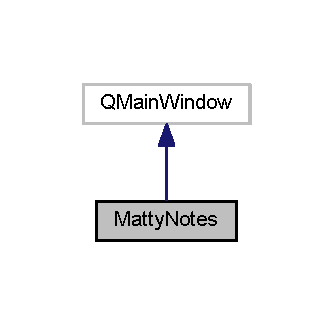
\includegraphics[width=160pt]{classMattyNotes__inherit__graph}
\end{center}
\end{figure}


Collaboration diagram for Matty\+Notes\+:
\nopagebreak
\begin{figure}[H]
\begin{center}
\leavevmode
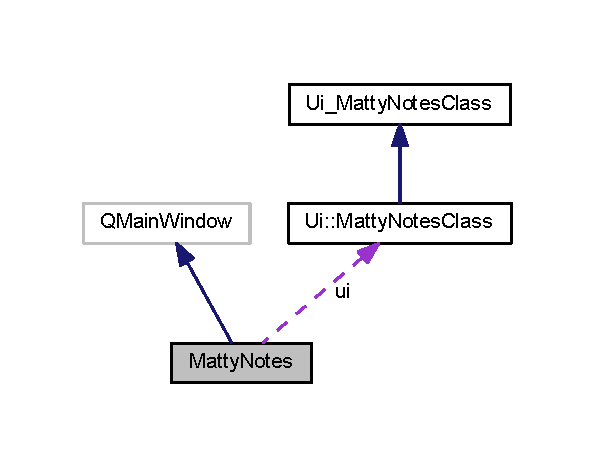
\includegraphics[width=286pt]{classMattyNotes__coll__graph}
\end{center}
\end{figure}
\subsection*{Public Member Functions}
\begin{DoxyCompactItemize}
\item 
\hyperlink{classMattyNotes_aa81db851f82183700abb0b7cd1ba2299}{Matty\+Notes} (Q\+Widget $\ast$parent=0)
\item 
\hyperlink{classMattyNotes_aff7466ee8047ed0293c62df37d245906}{$\sim$\+Matty\+Notes} ()
\end{DoxyCompactItemize}
\subsection*{Public Attributes}
\begin{DoxyCompactItemize}
\item 
Q\+Label $\ast$ \hyperlink{classMattyNotes_a855747a36f73f173f3d8f468c7196572}{header}
\item 
Q\+Push\+Button $\ast$ \hyperlink{classMattyNotes_ac72ba30ddc403561ed6904c4678caaaf}{close\+Window\+Button}
\item 
Q\+Push\+Button $\ast$ \hyperlink{classMattyNotes_a489ab2a613831dd27ba01eccf323235a}{maximize\+Window\+Button}
\item 
Q\+Push\+Button $\ast$ \hyperlink{classMattyNotes_a7d7fc5932df5ad6d5cee0fffe2a2feef}{minimize\+Window\+Button}
\item 
Q\+Tool\+Bar $\ast$ \hyperlink{classMattyNotes_ac780e9814bcce6c80afb9cc22d2b9af6}{Matty\+Tool\+Bar}
\item 
Q\+Push\+Button $\ast$ \hyperlink{classMattyNotes_a319952a9839f335ab9856b83369ea454}{add\+Note\+Button\+Temp}
\end{DoxyCompactItemize}
\subsection*{Private Slots}
\begin{DoxyCompactItemize}
\item 
void \hyperlink{classMattyNotes_a03ee529c5492bc8d73a8a93ecc32c394}{on\+\_\+add\+Note\+Button\+Temp\+\_\+clicked} ()
\item 
void \hyperlink{classMattyNotes_a63c0d10781a0acc57387682282aded37}{close\+Window} ()
\item 
void \hyperlink{classMattyNotes_a49cfcd1087c5f3c0c9f5ced2b7675e6f}{maximize\+Window} ()
\item 
void \hyperlink{classMattyNotes_a59034e42bf605fafd6b37e513b6f85fb}{minimize\+Window} ()
\end{DoxyCompactItemize}
\subsection*{Private Member Functions}
\begin{DoxyCompactItemize}
\item 
void \hyperlink{classMattyNotes_a4818a8cc2dbd824bc005034cb2656198}{mouse\+Press\+Event} (Q\+Mouse\+Event $\ast$event)
\item 
void \hyperlink{classMattyNotes_a0b9d1b50929a097d705e211b57fb12d0}{mouse\+Move\+Event} (Q\+Mouse\+Event $\ast$event)
\end{DoxyCompactItemize}
\subsection*{Private Attributes}
\begin{DoxyCompactItemize}
\item 
\hyperlink{classUi_1_1MattyNotesClass}{Ui\+::\+Matty\+Notes\+Class} \hyperlink{classMattyNotes_aa697392317715f04e4bc011090bebdb5}{ui}
\item 
int \hyperlink{classMattyNotes_a9c2352149386cb95946e3a8526c1ad2c}{m\+\_\+n\+Mouse\+Click\+\_\+\+X\+\_\+\+Coordinate}
\item 
int \hyperlink{classMattyNotes_aa4b9e6a5553ad49e4389340a783a85b9}{m\+\_\+n\+Mouse\+Click\+\_\+\+Y\+\_\+\+Coordinate}
\end{DoxyCompactItemize}


\subsection{Detailed Description}


Definition at line 11 of file mattynotes.\+h.



\subsection{Constructor \& Destructor Documentation}
\hypertarget{classMattyNotes_aa81db851f82183700abb0b7cd1ba2299}{}\label{classMattyNotes_aa81db851f82183700abb0b7cd1ba2299} 
\index{Matty\+Notes@{Matty\+Notes}!Matty\+Notes@{Matty\+Notes}}
\index{Matty\+Notes@{Matty\+Notes}!Matty\+Notes@{Matty\+Notes}}
\subsubsection{\texorpdfstring{Matty\+Notes()}{MattyNotes()}}
{\footnotesize\ttfamily Matty\+Notes\+::\+Matty\+Notes (\begin{DoxyParamCaption}\item[{Q\+Widget $\ast$}]{parent = {\ttfamily 0} }\end{DoxyParamCaption})}



Definition at line 11 of file mattynotes.\+cpp.

Here is the call graph for this function\+:
\nopagebreak
\begin{figure}[H]
\begin{center}
\leavevmode
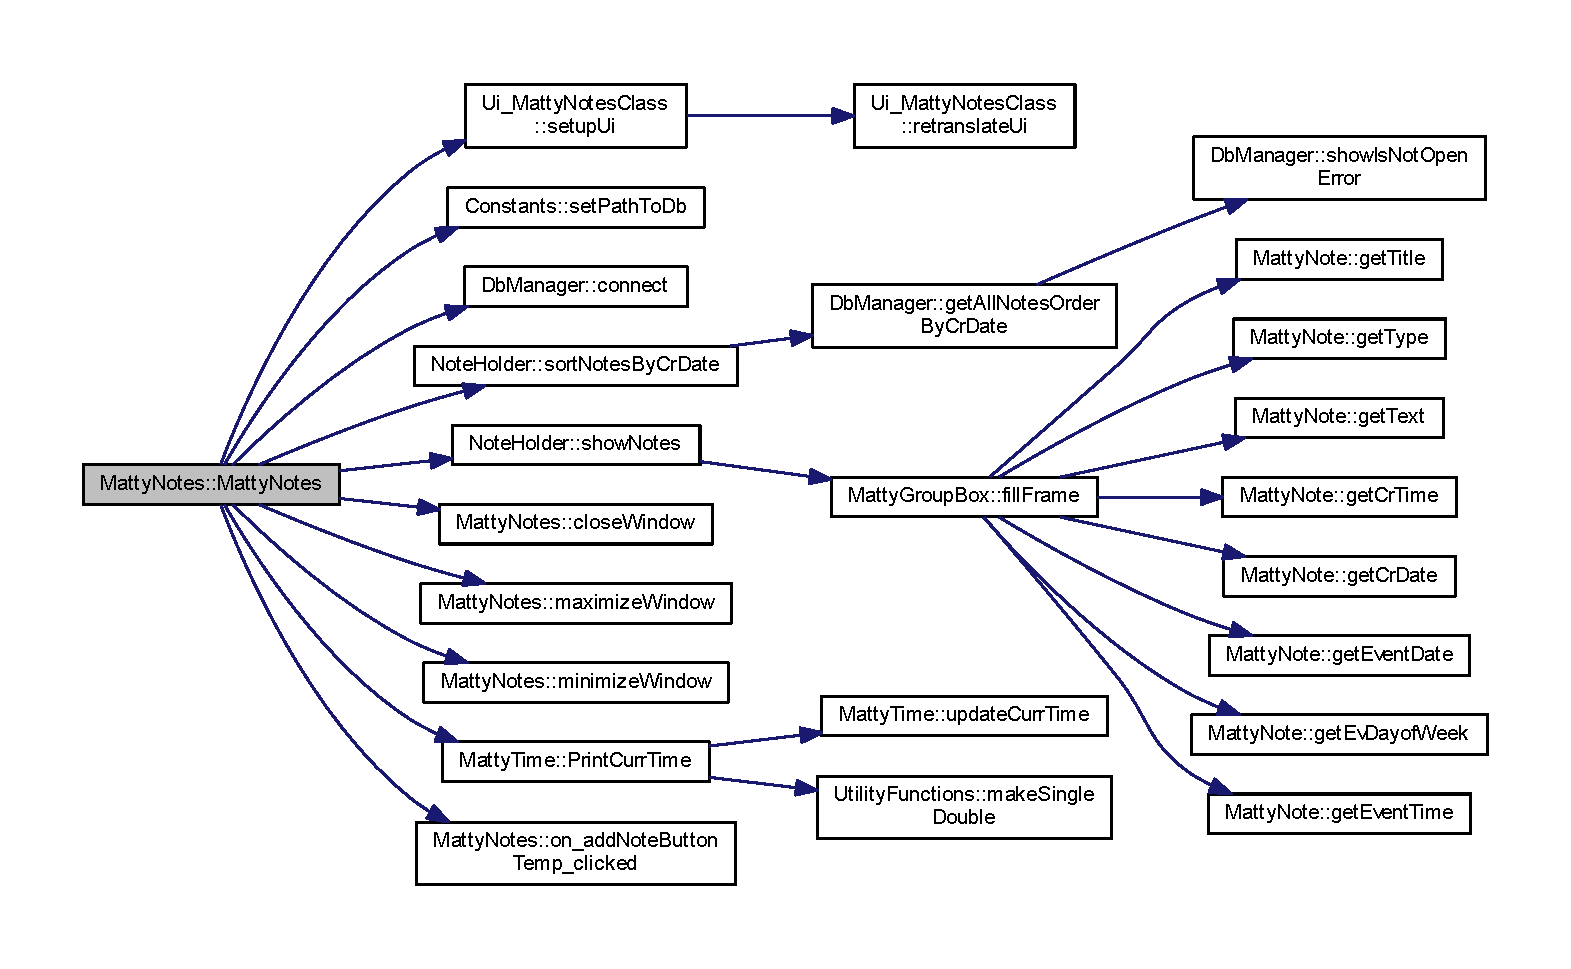
\includegraphics[width=350pt]{classMattyNotes_aa81db851f82183700abb0b7cd1ba2299_cgraph}
\end{center}
\end{figure}
\hypertarget{classMattyNotes_aff7466ee8047ed0293c62df37d245906}{}\label{classMattyNotes_aff7466ee8047ed0293c62df37d245906} 
\index{Matty\+Notes@{Matty\+Notes}!````~Matty\+Notes@{$\sim$\+Matty\+Notes}}
\index{````~Matty\+Notes@{$\sim$\+Matty\+Notes}!Matty\+Notes@{Matty\+Notes}}
\subsubsection{\texorpdfstring{$\sim$\+Matty\+Notes()}{~MattyNotes()}}
{\footnotesize\ttfamily Matty\+Notes\+::$\sim$\+Matty\+Notes (\begin{DoxyParamCaption}{ }\end{DoxyParamCaption})}



Definition at line 126 of file mattynotes.\+cpp.



\subsection{Member Function Documentation}
\hypertarget{classMattyNotes_a63c0d10781a0acc57387682282aded37}{}\label{classMattyNotes_a63c0d10781a0acc57387682282aded37} 
\index{Matty\+Notes@{Matty\+Notes}!close\+Window@{close\+Window}}
\index{close\+Window@{close\+Window}!Matty\+Notes@{Matty\+Notes}}
\subsubsection{\texorpdfstring{close\+Window}{closeWindow}}
{\footnotesize\ttfamily void Matty\+Notes\+::close\+Window (\begin{DoxyParamCaption}{ }\end{DoxyParamCaption})\hspace{0.3cm}{\ttfamily [private]}, {\ttfamily [slot]}}



Definition at line 146 of file mattynotes.\+cpp.

Here is the caller graph for this function\+:
\nopagebreak
\begin{figure}[H]
\begin{center}
\leavevmode
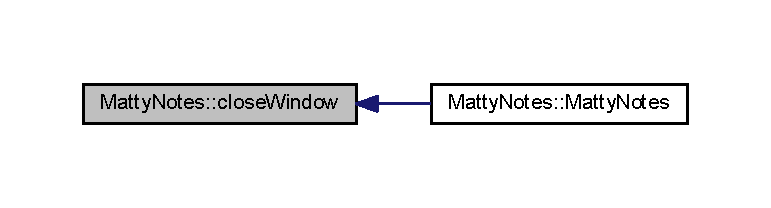
\includegraphics[width=350pt]{classMattyNotes_a63c0d10781a0acc57387682282aded37_icgraph}
\end{center}
\end{figure}
\hypertarget{classMattyNotes_a49cfcd1087c5f3c0c9f5ced2b7675e6f}{}\label{classMattyNotes_a49cfcd1087c5f3c0c9f5ced2b7675e6f} 
\index{Matty\+Notes@{Matty\+Notes}!maximize\+Window@{maximize\+Window}}
\index{maximize\+Window@{maximize\+Window}!Matty\+Notes@{Matty\+Notes}}
\subsubsection{\texorpdfstring{maximize\+Window}{maximizeWindow}}
{\footnotesize\ttfamily void Matty\+Notes\+::maximize\+Window (\begin{DoxyParamCaption}{ }\end{DoxyParamCaption})\hspace{0.3cm}{\ttfamily [private]}, {\ttfamily [slot]}}



Definition at line 151 of file mattynotes.\+cpp.

Here is the caller graph for this function\+:
\nopagebreak
\begin{figure}[H]
\begin{center}
\leavevmode
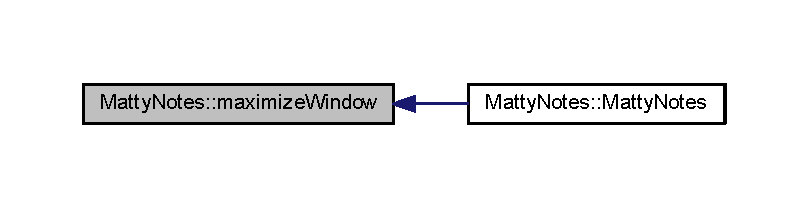
\includegraphics[width=350pt]{classMattyNotes_a49cfcd1087c5f3c0c9f5ced2b7675e6f_icgraph}
\end{center}
\end{figure}
\hypertarget{classMattyNotes_a59034e42bf605fafd6b37e513b6f85fb}{}\label{classMattyNotes_a59034e42bf605fafd6b37e513b6f85fb} 
\index{Matty\+Notes@{Matty\+Notes}!minimize\+Window@{minimize\+Window}}
\index{minimize\+Window@{minimize\+Window}!Matty\+Notes@{Matty\+Notes}}
\subsubsection{\texorpdfstring{minimize\+Window}{minimizeWindow}}
{\footnotesize\ttfamily void Matty\+Notes\+::minimize\+Window (\begin{DoxyParamCaption}{ }\end{DoxyParamCaption})\hspace{0.3cm}{\ttfamily [private]}, {\ttfamily [slot]}}



Definition at line 159 of file mattynotes.\+cpp.

Here is the caller graph for this function\+:
\nopagebreak
\begin{figure}[H]
\begin{center}
\leavevmode
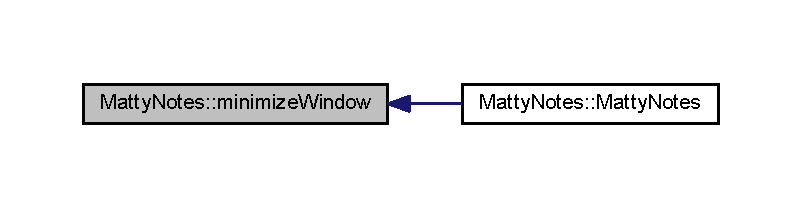
\includegraphics[width=350pt]{classMattyNotes_a59034e42bf605fafd6b37e513b6f85fb_icgraph}
\end{center}
\end{figure}
\hypertarget{classMattyNotes_a0b9d1b50929a097d705e211b57fb12d0}{}\label{classMattyNotes_a0b9d1b50929a097d705e211b57fb12d0} 
\index{Matty\+Notes@{Matty\+Notes}!mouse\+Move\+Event@{mouse\+Move\+Event}}
\index{mouse\+Move\+Event@{mouse\+Move\+Event}!Matty\+Notes@{Matty\+Notes}}
\subsubsection{\texorpdfstring{mouse\+Move\+Event()}{mouseMoveEvent()}}
{\footnotesize\ttfamily void Matty\+Notes\+::mouse\+Move\+Event (\begin{DoxyParamCaption}\item[{Q\+Mouse\+Event $\ast$}]{event }\end{DoxyParamCaption})\hspace{0.3cm}{\ttfamily [private]}}



Definition at line 175 of file mattynotes.\+cpp.

\hypertarget{classMattyNotes_a4818a8cc2dbd824bc005034cb2656198}{}\label{classMattyNotes_a4818a8cc2dbd824bc005034cb2656198} 
\index{Matty\+Notes@{Matty\+Notes}!mouse\+Press\+Event@{mouse\+Press\+Event}}
\index{mouse\+Press\+Event@{mouse\+Press\+Event}!Matty\+Notes@{Matty\+Notes}}
\subsubsection{\texorpdfstring{mouse\+Press\+Event()}{mousePressEvent()}}
{\footnotesize\ttfamily void Matty\+Notes\+::mouse\+Press\+Event (\begin{DoxyParamCaption}\item[{Q\+Mouse\+Event $\ast$}]{event }\end{DoxyParamCaption})\hspace{0.3cm}{\ttfamily [private]}}



Definition at line 169 of file mattynotes.\+cpp.

\hypertarget{classMattyNotes_a03ee529c5492bc8d73a8a93ecc32c394}{}\label{classMattyNotes_a03ee529c5492bc8d73a8a93ecc32c394} 
\index{Matty\+Notes@{Matty\+Notes}!on\+\_\+add\+Note\+Button\+Temp\+\_\+clicked@{on\+\_\+add\+Note\+Button\+Temp\+\_\+clicked}}
\index{on\+\_\+add\+Note\+Button\+Temp\+\_\+clicked@{on\+\_\+add\+Note\+Button\+Temp\+\_\+clicked}!Matty\+Notes@{Matty\+Notes}}
\subsubsection{\texorpdfstring{on\+\_\+add\+Note\+Button\+Temp\+\_\+clicked}{on\_addNoteButtonTemp\_clicked}}
{\footnotesize\ttfamily void Matty\+Notes\+::on\+\_\+add\+Note\+Button\+Temp\+\_\+clicked (\begin{DoxyParamCaption}{ }\end{DoxyParamCaption})\hspace{0.3cm}{\ttfamily [private]}, {\ttfamily [slot]}}



Definition at line 139 of file mattynotes.\+cpp.

Here is the caller graph for this function\+:
\nopagebreak
\begin{figure}[H]
\begin{center}
\leavevmode
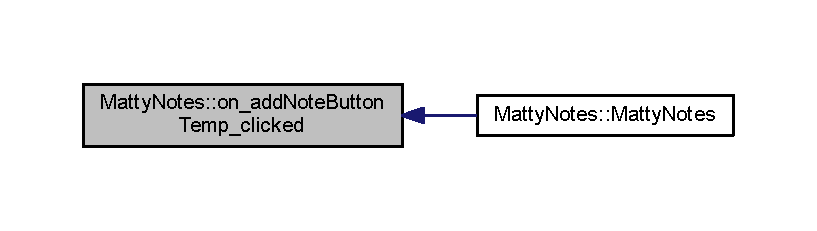
\includegraphics[width=350pt]{classMattyNotes_a03ee529c5492bc8d73a8a93ecc32c394_icgraph}
\end{center}
\end{figure}


\subsection{Member Data Documentation}
\hypertarget{classMattyNotes_a319952a9839f335ab9856b83369ea454}{}\label{classMattyNotes_a319952a9839f335ab9856b83369ea454} 
\index{Matty\+Notes@{Matty\+Notes}!add\+Note\+Button\+Temp@{add\+Note\+Button\+Temp}}
\index{add\+Note\+Button\+Temp@{add\+Note\+Button\+Temp}!Matty\+Notes@{Matty\+Notes}}
\subsubsection{\texorpdfstring{add\+Note\+Button\+Temp}{addNoteButtonTemp}}
{\footnotesize\ttfamily Q\+Push\+Button$\ast$ Matty\+Notes\+::add\+Note\+Button\+Temp}



Definition at line 23 of file mattynotes.\+h.

\hypertarget{classMattyNotes_ac72ba30ddc403561ed6904c4678caaaf}{}\label{classMattyNotes_ac72ba30ddc403561ed6904c4678caaaf} 
\index{Matty\+Notes@{Matty\+Notes}!close\+Window\+Button@{close\+Window\+Button}}
\index{close\+Window\+Button@{close\+Window\+Button}!Matty\+Notes@{Matty\+Notes}}
\subsubsection{\texorpdfstring{close\+Window\+Button}{closeWindowButton}}
{\footnotesize\ttfamily Q\+Push\+Button$\ast$ Matty\+Notes\+::close\+Window\+Button}



Definition at line 19 of file mattynotes.\+h.

\hypertarget{classMattyNotes_a855747a36f73f173f3d8f468c7196572}{}\label{classMattyNotes_a855747a36f73f173f3d8f468c7196572} 
\index{Matty\+Notes@{Matty\+Notes}!header@{header}}
\index{header@{header}!Matty\+Notes@{Matty\+Notes}}
\subsubsection{\texorpdfstring{header}{header}}
{\footnotesize\ttfamily Q\+Label$\ast$ Matty\+Notes\+::header}



Definition at line 18 of file mattynotes.\+h.

\hypertarget{classMattyNotes_a9c2352149386cb95946e3a8526c1ad2c}{}\label{classMattyNotes_a9c2352149386cb95946e3a8526c1ad2c} 
\index{Matty\+Notes@{Matty\+Notes}!m\+\_\+n\+Mouse\+Click\+\_\+\+X\+\_\+\+Coordinate@{m\+\_\+n\+Mouse\+Click\+\_\+\+X\+\_\+\+Coordinate}}
\index{m\+\_\+n\+Mouse\+Click\+\_\+\+X\+\_\+\+Coordinate@{m\+\_\+n\+Mouse\+Click\+\_\+\+X\+\_\+\+Coordinate}!Matty\+Notes@{Matty\+Notes}}
\subsubsection{\texorpdfstring{m\+\_\+n\+Mouse\+Click\+\_\+\+X\+\_\+\+Coordinate}{m\_nMouseClick\_X\_Coordinate}}
{\footnotesize\ttfamily int Matty\+Notes\+::m\+\_\+n\+Mouse\+Click\+\_\+\+X\+\_\+\+Coordinate\hspace{0.3cm}{\ttfamily [private]}}



Definition at line 32 of file mattynotes.\+h.

\hypertarget{classMattyNotes_aa4b9e6a5553ad49e4389340a783a85b9}{}\label{classMattyNotes_aa4b9e6a5553ad49e4389340a783a85b9} 
\index{Matty\+Notes@{Matty\+Notes}!m\+\_\+n\+Mouse\+Click\+\_\+\+Y\+\_\+\+Coordinate@{m\+\_\+n\+Mouse\+Click\+\_\+\+Y\+\_\+\+Coordinate}}
\index{m\+\_\+n\+Mouse\+Click\+\_\+\+Y\+\_\+\+Coordinate@{m\+\_\+n\+Mouse\+Click\+\_\+\+Y\+\_\+\+Coordinate}!Matty\+Notes@{Matty\+Notes}}
\subsubsection{\texorpdfstring{m\+\_\+n\+Mouse\+Click\+\_\+\+Y\+\_\+\+Coordinate}{m\_nMouseClick\_Y\_Coordinate}}
{\footnotesize\ttfamily int Matty\+Notes\+::m\+\_\+n\+Mouse\+Click\+\_\+\+Y\+\_\+\+Coordinate\hspace{0.3cm}{\ttfamily [private]}}



Definition at line 33 of file mattynotes.\+h.

\hypertarget{classMattyNotes_ac780e9814bcce6c80afb9cc22d2b9af6}{}\label{classMattyNotes_ac780e9814bcce6c80afb9cc22d2b9af6} 
\index{Matty\+Notes@{Matty\+Notes}!Matty\+Tool\+Bar@{Matty\+Tool\+Bar}}
\index{Matty\+Tool\+Bar@{Matty\+Tool\+Bar}!Matty\+Notes@{Matty\+Notes}}
\subsubsection{\texorpdfstring{Matty\+Tool\+Bar}{MattyToolBar}}
{\footnotesize\ttfamily Q\+Tool\+Bar$\ast$ Matty\+Notes\+::\+Matty\+Tool\+Bar}



Definition at line 22 of file mattynotes.\+h.

\hypertarget{classMattyNotes_a489ab2a613831dd27ba01eccf323235a}{}\label{classMattyNotes_a489ab2a613831dd27ba01eccf323235a} 
\index{Matty\+Notes@{Matty\+Notes}!maximize\+Window\+Button@{maximize\+Window\+Button}}
\index{maximize\+Window\+Button@{maximize\+Window\+Button}!Matty\+Notes@{Matty\+Notes}}
\subsubsection{\texorpdfstring{maximize\+Window\+Button}{maximizeWindowButton}}
{\footnotesize\ttfamily Q\+Push\+Button$\ast$ Matty\+Notes\+::maximize\+Window\+Button}



Definition at line 20 of file mattynotes.\+h.

\hypertarget{classMattyNotes_a7d7fc5932df5ad6d5cee0fffe2a2feef}{}\label{classMattyNotes_a7d7fc5932df5ad6d5cee0fffe2a2feef} 
\index{Matty\+Notes@{Matty\+Notes}!minimize\+Window\+Button@{minimize\+Window\+Button}}
\index{minimize\+Window\+Button@{minimize\+Window\+Button}!Matty\+Notes@{Matty\+Notes}}
\subsubsection{\texorpdfstring{minimize\+Window\+Button}{minimizeWindowButton}}
{\footnotesize\ttfamily Q\+Push\+Button$\ast$ Matty\+Notes\+::minimize\+Window\+Button}



Definition at line 21 of file mattynotes.\+h.

\hypertarget{classMattyNotes_aa697392317715f04e4bc011090bebdb5}{}\label{classMattyNotes_aa697392317715f04e4bc011090bebdb5} 
\index{Matty\+Notes@{Matty\+Notes}!ui@{ui}}
\index{ui@{ui}!Matty\+Notes@{Matty\+Notes}}
\subsubsection{\texorpdfstring{ui}{ui}}
{\footnotesize\ttfamily \hyperlink{classUi_1_1MattyNotesClass}{Ui\+::\+Matty\+Notes\+Class} Matty\+Notes\+::ui\hspace{0.3cm}{\ttfamily [private]}}



Definition at line 29 of file mattynotes.\+h.



The documentation for this class was generated from the following files\+:\begin{DoxyCompactItemize}
\item 
C\+:/\+Users/\+Ogrigorieva/\+Visual Studio 2015/\+Projects/\+Personal/\+Matty\+Notes/\hyperlink{mattynotes_8h}{mattynotes.\+h}\item 
C\+:/\+Users/\+Ogrigorieva/\+Visual Studio 2015/\+Projects/\+Personal/\+Matty\+Notes/\hyperlink{mattynotes_8cpp}{mattynotes.\+cpp}\end{DoxyCompactItemize}

\hypertarget{classUi_1_1MattyNotesClass}{}\section{Ui\+:\+:Matty\+Notes\+Class Class Reference}
\label{classUi_1_1MattyNotesClass}\index{Ui\+::\+Matty\+Notes\+Class@{Ui\+::\+Matty\+Notes\+Class}}


{\ttfamily \#include $<$ui\+\_\+mattynotes.\+h$>$}



Inheritance diagram for Ui\+:\+:Matty\+Notes\+Class\+:
% FIG 0


Collaboration diagram for Ui\+:\+:Matty\+Notes\+Class\+:
% FIG 1
\subsection*{Additional Inherited Members}


\subsection{Detailed Description}


Definition at line 286 of file ui\+\_\+mattynotes.\+h.



The documentation for this class was generated from the following file\+:\begin{DoxyCompactItemize}
\item 
C\+:/\+Users/\+Ogrigorieva/\+Visual Studio 2015/\+Projects/\+Personal/\+Matty\+Notes/\+Generated\+Files/\hyperlink{ui__mattynotes_8h}{ui\+\_\+mattynotes.\+h}\end{DoxyCompactItemize}

\hypertarget{classMattySettings}{}\section{Matty\+Settings Class Reference}
\label{classMattySettings}\index{Matty\+Settings@{Matty\+Settings}}


{\ttfamily \#include $<$mattysettings.\+h$>$}



Inheritance diagram for Matty\+Settings\+:
\nopagebreak
\begin{figure}[H]
\begin{center}
\leavevmode
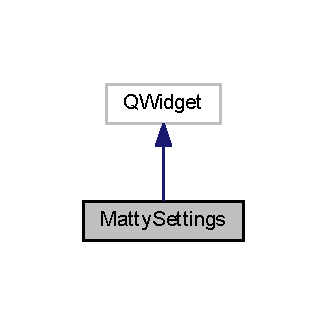
\includegraphics[width=157pt]{classMattySettings__inherit__graph}
\end{center}
\end{figure}


Collaboration diagram for Matty\+Settings\+:
\nopagebreak
\begin{figure}[H]
\begin{center}
\leavevmode
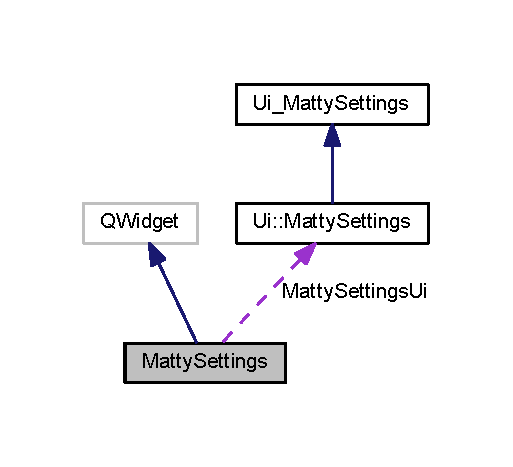
\includegraphics[width=246pt]{classMattySettings__coll__graph}
\end{center}
\end{figure}
\subsection*{Public Member Functions}
\begin{DoxyCompactItemize}
\item 
\hyperlink{classMattySettings_a0d5b0f74bacfcad4f084772a081294a9}{Matty\+Settings} (Q\+Widget $\ast$parent=0)
\item 
\hyperlink{classMattySettings_a361e58579542394627a34f07f408aa3a}{$\sim$\+Matty\+Settings} ()
\end{DoxyCompactItemize}
\subsection*{Private Member Functions}
\begin{DoxyCompactItemize}
\item 
void \hyperlink{classMattySettings_aedf4cc84f37e25a7704e1ced6c18df95}{mouse\+Press\+Event} (Q\+Mouse\+Event $\ast$event)
\item 
void \hyperlink{classMattySettings_a0d151b91e1d79229d6ae0addf858c0d8}{mouse\+Move\+Event} (Q\+Mouse\+Event $\ast$event)
\end{DoxyCompactItemize}
\subsection*{Private Attributes}
\begin{DoxyCompactItemize}
\item 
\hyperlink{classUi_1_1MattySettings}{Ui\+::\+Matty\+Settings} \hyperlink{classMattySettings_a6974b17b34c30385f6b503f40b460ea1}{Matty\+Settings\+Ui}
\item 
int \hyperlink{classMattySettings_aa1c8051298eee4d2e77a93af3ddeb9d0}{m\+\_\+n\+Mouse\+Click\+\_\+\+X\+\_\+\+Coordinate}
\item 
int \hyperlink{classMattySettings_a622b01c6b81a35e28b414079eaff132e}{m\+\_\+n\+Mouse\+Click\+\_\+\+Y\+\_\+\+Coordinate}
\end{DoxyCompactItemize}


\subsection{Detailed Description}


Definition at line 11 of file mattysettings.\+h.



\subsection{Constructor \& Destructor Documentation}
\hypertarget{classMattySettings_a0d5b0f74bacfcad4f084772a081294a9}{}\label{classMattySettings_a0d5b0f74bacfcad4f084772a081294a9} 
\index{Matty\+Settings@{Matty\+Settings}!Matty\+Settings@{Matty\+Settings}}
\index{Matty\+Settings@{Matty\+Settings}!Matty\+Settings@{Matty\+Settings}}
\subsubsection{\texorpdfstring{Matty\+Settings()}{MattySettings()}}
{\footnotesize\ttfamily Matty\+Settings\+::\+Matty\+Settings (\begin{DoxyParamCaption}\item[{Q\+Widget $\ast$}]{parent = {\ttfamily 0} }\end{DoxyParamCaption})}



Definition at line 4 of file mattysettings.\+cpp.

Here is the call graph for this function\+:
\nopagebreak
\begin{figure}[H]
\begin{center}
\leavevmode
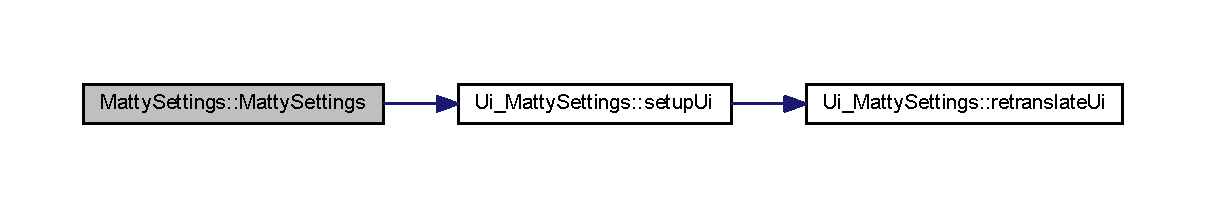
\includegraphics[width=350pt]{classMattySettings_a0d5b0f74bacfcad4f084772a081294a9_cgraph}
\end{center}
\end{figure}
\hypertarget{classMattySettings_a361e58579542394627a34f07f408aa3a}{}\label{classMattySettings_a361e58579542394627a34f07f408aa3a} 
\index{Matty\+Settings@{Matty\+Settings}!````~Matty\+Settings@{$\sim$\+Matty\+Settings}}
\index{````~Matty\+Settings@{$\sim$\+Matty\+Settings}!Matty\+Settings@{Matty\+Settings}}
\subsubsection{\texorpdfstring{$\sim$\+Matty\+Settings()}{~MattySettings()}}
{\footnotesize\ttfamily Matty\+Settings\+::$\sim$\+Matty\+Settings (\begin{DoxyParamCaption}{ }\end{DoxyParamCaption})}



Definition at line 14 of file mattysettings.\+cpp.



\subsection{Member Function Documentation}
\hypertarget{classMattySettings_a0d151b91e1d79229d6ae0addf858c0d8}{}\label{classMattySettings_a0d151b91e1d79229d6ae0addf858c0d8} 
\index{Matty\+Settings@{Matty\+Settings}!mouse\+Move\+Event@{mouse\+Move\+Event}}
\index{mouse\+Move\+Event@{mouse\+Move\+Event}!Matty\+Settings@{Matty\+Settings}}
\subsubsection{\texorpdfstring{mouse\+Move\+Event()}{mouseMoveEvent()}}
{\footnotesize\ttfamily void Matty\+Settings\+::mouse\+Move\+Event (\begin{DoxyParamCaption}\item[{Q\+Mouse\+Event $\ast$}]{event }\end{DoxyParamCaption})\hspace{0.3cm}{\ttfamily [private]}}



Definition at line 25 of file mattysettings.\+cpp.

\hypertarget{classMattySettings_aedf4cc84f37e25a7704e1ced6c18df95}{}\label{classMattySettings_aedf4cc84f37e25a7704e1ced6c18df95} 
\index{Matty\+Settings@{Matty\+Settings}!mouse\+Press\+Event@{mouse\+Press\+Event}}
\index{mouse\+Press\+Event@{mouse\+Press\+Event}!Matty\+Settings@{Matty\+Settings}}
\subsubsection{\texorpdfstring{mouse\+Press\+Event()}{mousePressEvent()}}
{\footnotesize\ttfamily void Matty\+Settings\+::mouse\+Press\+Event (\begin{DoxyParamCaption}\item[{Q\+Mouse\+Event $\ast$}]{event }\end{DoxyParamCaption})\hspace{0.3cm}{\ttfamily [private]}}



Definition at line 19 of file mattysettings.\+cpp.



\subsection{Member Data Documentation}
\hypertarget{classMattySettings_aa1c8051298eee4d2e77a93af3ddeb9d0}{}\label{classMattySettings_aa1c8051298eee4d2e77a93af3ddeb9d0} 
\index{Matty\+Settings@{Matty\+Settings}!m\+\_\+n\+Mouse\+Click\+\_\+\+X\+\_\+\+Coordinate@{m\+\_\+n\+Mouse\+Click\+\_\+\+X\+\_\+\+Coordinate}}
\index{m\+\_\+n\+Mouse\+Click\+\_\+\+X\+\_\+\+Coordinate@{m\+\_\+n\+Mouse\+Click\+\_\+\+X\+\_\+\+Coordinate}!Matty\+Settings@{Matty\+Settings}}
\subsubsection{\texorpdfstring{m\+\_\+n\+Mouse\+Click\+\_\+\+X\+\_\+\+Coordinate}{m\_nMouseClick\_X\_Coordinate}}
{\footnotesize\ttfamily int Matty\+Settings\+::m\+\_\+n\+Mouse\+Click\+\_\+\+X\+\_\+\+Coordinate\hspace{0.3cm}{\ttfamily [private]}}



Definition at line 22 of file mattysettings.\+h.

\hypertarget{classMattySettings_a622b01c6b81a35e28b414079eaff132e}{}\label{classMattySettings_a622b01c6b81a35e28b414079eaff132e} 
\index{Matty\+Settings@{Matty\+Settings}!m\+\_\+n\+Mouse\+Click\+\_\+\+Y\+\_\+\+Coordinate@{m\+\_\+n\+Mouse\+Click\+\_\+\+Y\+\_\+\+Coordinate}}
\index{m\+\_\+n\+Mouse\+Click\+\_\+\+Y\+\_\+\+Coordinate@{m\+\_\+n\+Mouse\+Click\+\_\+\+Y\+\_\+\+Coordinate}!Matty\+Settings@{Matty\+Settings}}
\subsubsection{\texorpdfstring{m\+\_\+n\+Mouse\+Click\+\_\+\+Y\+\_\+\+Coordinate}{m\_nMouseClick\_Y\_Coordinate}}
{\footnotesize\ttfamily int Matty\+Settings\+::m\+\_\+n\+Mouse\+Click\+\_\+\+Y\+\_\+\+Coordinate\hspace{0.3cm}{\ttfamily [private]}}



Definition at line 23 of file mattysettings.\+h.

\hypertarget{classMattySettings_a6974b17b34c30385f6b503f40b460ea1}{}\label{classMattySettings_a6974b17b34c30385f6b503f40b460ea1} 
\index{Matty\+Settings@{Matty\+Settings}!Matty\+Settings\+Ui@{Matty\+Settings\+Ui}}
\index{Matty\+Settings\+Ui@{Matty\+Settings\+Ui}!Matty\+Settings@{Matty\+Settings}}
\subsubsection{\texorpdfstring{Matty\+Settings\+Ui}{MattySettingsUi}}
{\footnotesize\ttfamily \hyperlink{classUi_1_1MattySettings}{Ui\+::\+Matty\+Settings} Matty\+Settings\+::\+Matty\+Settings\+Ui\hspace{0.3cm}{\ttfamily [private]}}



Definition at line 19 of file mattysettings.\+h.



The documentation for this class was generated from the following files\+:\begin{DoxyCompactItemize}
\item 
C\+:/\+Users/\+Ogrigorieva/\+Visual Studio 2015/\+Projects/\+Personal/\+Matty\+Notes/\hyperlink{mattysettings_8h}{mattysettings.\+h}\item 
C\+:/\+Users/\+Ogrigorieva/\+Visual Studio 2015/\+Projects/\+Personal/\+Matty\+Notes/\hyperlink{mattysettings_8cpp}{mattysettings.\+cpp}\end{DoxyCompactItemize}

\hypertarget{classUi_1_1MattySettings}{}\section{Ui\+:\+:Matty\+Settings Class Reference}
\label{classUi_1_1MattySettings}\index{Ui\+::\+Matty\+Settings@{Ui\+::\+Matty\+Settings}}


{\ttfamily \#include $<$ui\+\_\+mattysettings.\+h$>$}



Inheritance diagram for Ui\+:\+:Matty\+Settings\+:
% FIG 0


Collaboration diagram for Ui\+:\+:Matty\+Settings\+:
% FIG 1
\subsection*{Additional Inherited Members}


\subsection{Detailed Description}


Definition at line 48 of file ui\+\_\+mattysettings.\+h.



The documentation for this class was generated from the following file\+:\begin{DoxyCompactItemize}
\item 
C\+:/\+Users/\+Ogrigorieva/\+Visual Studio 2015/\+Projects/\+Personal/\+Matty\+Notes/\+Generated\+Files/\hyperlink{ui__mattysettings_8h}{ui\+\_\+mattysettings.\+h}\end{DoxyCompactItemize}

\hypertarget{classMattyTime}{}\section{Matty\+Time Class Reference}
\label{classMattyTime}\index{Matty\+Time@{Matty\+Time}}


{\ttfamily \#include $<$Matty\+Time.\+h$>$}



Collaboration diagram for Matty\+Time\+:
\nopagebreak
\begin{figure}[H]
\begin{center}
\leavevmode
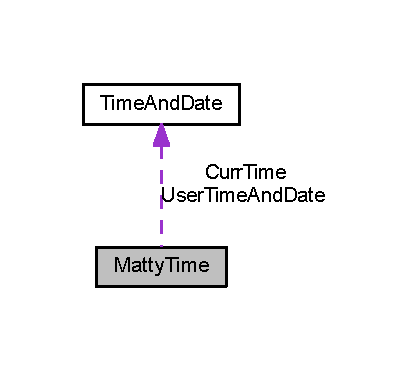
\includegraphics[width=197pt]{classMattyTime__coll__graph}
\end{center}
\end{figure}
\subsection*{Public Member Functions}
\begin{DoxyCompactItemize}
\item 
\hyperlink{classMattyTime_aebf245aa0b578982cad3f679ea5348cd}{Matty\+Time} ()
\item 
void \hyperlink{classMattyTime_a858357a5febc483c27f9bbf96b83b175}{set\+User\+Date\+And\+Time} (int second)
\item 
void \hyperlink{classMattyTime_a60828ca950added6776f53ca3ea047fc}{set\+User\+Date\+And\+Time} (int hour, int minute)
\item 
void \hyperlink{classMattyTime_ac6d00b726df1a8c493452dfc52332f6f}{set\+User\+Date\+And\+Time} (int day, int month, int year)
\item 
void \hyperlink{classMattyTime_a34af1776506d7a99387db16982987e1c}{set\+User\+Date\+And\+Time} (int hour, int minute, int day, int month, int year)
\item 
void \hyperlink{classMattyTime_ae470fb0341c517348ec3ea7d606f67c5}{set\+User\+Date\+And\+Time} (\hyperlink{structTimeAndDate}{Time\+And\+Date} Time\+Date)
\item 
\hyperlink{structTimeAndDate}{Time\+And\+Date} \hyperlink{classMattyTime_ac2f2f818e4c476cc11f9c13e97cacfae}{Get\+User\+Date\+And\+Time} ()
\item 
Q\+String \hyperlink{classMattyTime_a9cbf666ccbe45a8ca45f9ffc42d5102c}{Print\+User\+Time} ()
\item 
Q\+String \hyperlink{classMattyTime_a3fda0198071ebc95afe2d4405dd9c55e}{Print\+User\+Time\+Full} ()
\item 
Q\+String \hyperlink{classMattyTime_a646278576993d7ed05af67aee6ac96cb}{Print\+User\+Date} ()
\item 
Q\+String \hyperlink{classMattyTime_afa30c1dd3bae1e8f50e816803f39d1c4}{Print\+User\+Time\+And\+Date} ()
\item 
Q\+String \hyperlink{classMattyTime_a6bcaa1f4975d99ab2f9025076de5ef99}{Print\+User\+Time\+Full\+And\+Date} ()
\item 
void \hyperlink{classMattyTime_afef585f71d11eed7777065af8ca0e9f0}{set\+User\+Time\+And\+Date\+Now} ()
\item 
void \hyperlink{classMattyTime_a6ae52c957bcf12e92624e09db890ce21}{set\+User\+Time\+And\+Date\+Null} ()
\item 
void \hyperlink{classMattyTime_a12b0e0b9c4d45248da89e2d4078d4d08}{set\+User\+Day\+Of\+Week} ()
\item 
Q\+String \hyperlink{classMattyTime_ad2f12ac7d1a959ee9e19a4eac30484fd}{get\+User\+Day\+Of\+Week} ()
\item 
\hyperlink{classMattyTime_acb302c8f6c5215dc974f87753ed2fd61}{$\sim$\+Matty\+Time} ()
\end{DoxyCompactItemize}
\subsection*{Static Public Member Functions}
\begin{DoxyCompactItemize}
\item 
static void \hyperlink{classMattyTime_a52a7500e419fe56d10ddf2715fc96d06}{update\+Curr\+Time} ()
\item 
static \hyperlink{structTimeAndDate}{Time\+And\+Date} \hyperlink{classMattyTime_a64fff9c9a7da58881a4c0cc1a2ac84f7}{get\+Curr\+Time} ()
\item 
static Q\+String \hyperlink{classMattyTime_ac5ecfd2ff5329b3476906b39bbf02ae3}{Print\+Curr\+Time} ()
\item 
static Q\+String \hyperlink{classMattyTime_a9d3500ad88197ee8e2db9f36aec1a266}{Print\+Curr\+Time\+Full} ()
\item 
static Q\+String \hyperlink{classMattyTime_af87198affde58c9f254dbf1601fb9f1e}{Print\+Curr\+Date} ()
\item 
static Q\+String \hyperlink{classMattyTime_a96805256f90a469aa22824a1e2dd219d}{Print\+Curr\+Time\+And\+Date} ()
\item 
static Q\+String \hyperlink{classMattyTime_a82a6b06fa496b4d0f9b8d6e11d5b03c8}{Print\+Curr\+Time\+Full\+And\+Date} ()
\end{DoxyCompactItemize}
\subsection*{Public Attributes}
\begin{DoxyCompactItemize}
\item 
\hyperlink{structTimeAndDate}{Time\+And\+Date} \hyperlink{classMattyTime_a7a1ceab576011e56405b49d7bd81e475}{User\+Time\+And\+Date}
\end{DoxyCompactItemize}
\subsection*{Static Public Attributes}
\begin{DoxyCompactItemize}
\item 
static \hyperlink{structTimeAndDate}{Time\+And\+Date} \hyperlink{classMattyTime_a458337456f43243073ae78976e86618f}{Curr\+Time}
\end{DoxyCompactItemize}


\subsection{Detailed Description}


Definition at line 36 of file Matty\+Time.\+h.



\subsection{Constructor \& Destructor Documentation}
\hypertarget{classMattyTime_aebf245aa0b578982cad3f679ea5348cd}{}\label{classMattyTime_aebf245aa0b578982cad3f679ea5348cd} 
\index{Matty\+Time@{Matty\+Time}!Matty\+Time@{Matty\+Time}}
\index{Matty\+Time@{Matty\+Time}!Matty\+Time@{Matty\+Time}}
\subsubsection{\texorpdfstring{Matty\+Time()}{MattyTime()}}
{\footnotesize\ttfamily Matty\+Time\+::\+Matty\+Time (\begin{DoxyParamCaption}{ }\end{DoxyParamCaption})}



Definition at line 22 of file Matty\+Time.\+cpp.

\hypertarget{classMattyTime_acb302c8f6c5215dc974f87753ed2fd61}{}\label{classMattyTime_acb302c8f6c5215dc974f87753ed2fd61} 
\index{Matty\+Time@{Matty\+Time}!````~Matty\+Time@{$\sim$\+Matty\+Time}}
\index{````~Matty\+Time@{$\sim$\+Matty\+Time}!Matty\+Time@{Matty\+Time}}
\subsubsection{\texorpdfstring{$\sim$\+Matty\+Time()}{~MattyTime()}}
{\footnotesize\ttfamily Matty\+Time\+::$\sim$\+Matty\+Time (\begin{DoxyParamCaption}{ }\end{DoxyParamCaption})}



Definition at line 250 of file Matty\+Time.\+cpp.



\subsection{Member Function Documentation}
\hypertarget{classMattyTime_a64fff9c9a7da58881a4c0cc1a2ac84f7}{}\label{classMattyTime_a64fff9c9a7da58881a4c0cc1a2ac84f7} 
\index{Matty\+Time@{Matty\+Time}!get\+Curr\+Time@{get\+Curr\+Time}}
\index{get\+Curr\+Time@{get\+Curr\+Time}!Matty\+Time@{Matty\+Time}}
\subsubsection{\texorpdfstring{get\+Curr\+Time()}{getCurrTime()}}
{\footnotesize\ttfamily \hyperlink{structTimeAndDate}{Time\+And\+Date} Matty\+Time\+::get\+Curr\+Time (\begin{DoxyParamCaption}{ }\end{DoxyParamCaption})\hspace{0.3cm}{\ttfamily [static]}}



Definition at line 41 of file Matty\+Time.\+cpp.

Here is the call graph for this function\+:
\nopagebreak
\begin{figure}[H]
\begin{center}
\leavevmode
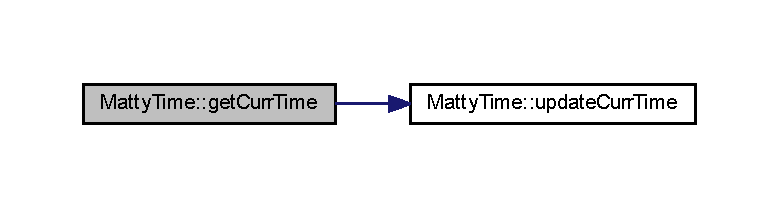
\includegraphics[width=350pt]{classMattyTime_a64fff9c9a7da58881a4c0cc1a2ac84f7_cgraph}
\end{center}
\end{figure}
\hypertarget{classMattyTime_ac2f2f818e4c476cc11f9c13e97cacfae}{}\label{classMattyTime_ac2f2f818e4c476cc11f9c13e97cacfae} 
\index{Matty\+Time@{Matty\+Time}!Get\+User\+Date\+And\+Time@{Get\+User\+Date\+And\+Time}}
\index{Get\+User\+Date\+And\+Time@{Get\+User\+Date\+And\+Time}!Matty\+Time@{Matty\+Time}}
\subsubsection{\texorpdfstring{Get\+User\+Date\+And\+Time()}{GetUserDateAndTime()}}
{\footnotesize\ttfamily \hyperlink{structTimeAndDate}{Time\+And\+Date} Matty\+Time\+::\+Get\+User\+Date\+And\+Time (\begin{DoxyParamCaption}{ }\end{DoxyParamCaption})}



Definition at line 85 of file Matty\+Time.\+cpp.

\hypertarget{classMattyTime_ad2f12ac7d1a959ee9e19a4eac30484fd}{}\label{classMattyTime_ad2f12ac7d1a959ee9e19a4eac30484fd} 
\index{Matty\+Time@{Matty\+Time}!get\+User\+Day\+Of\+Week@{get\+User\+Day\+Of\+Week}}
\index{get\+User\+Day\+Of\+Week@{get\+User\+Day\+Of\+Week}!Matty\+Time@{Matty\+Time}}
\subsubsection{\texorpdfstring{get\+User\+Day\+Of\+Week()}{getUserDayOfWeek()}}
{\footnotesize\ttfamily Q\+String Matty\+Time\+::get\+User\+Day\+Of\+Week (\begin{DoxyParamCaption}{ }\end{DoxyParamCaption})}



Definition at line 219 of file Matty\+Time.\+cpp.

Here is the caller graph for this function\+:
\nopagebreak
\begin{figure}[H]
\begin{center}
\leavevmode
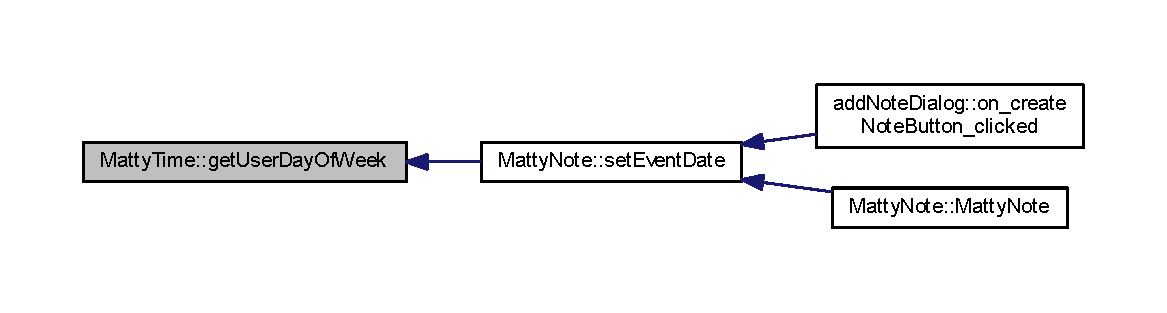
\includegraphics[width=350pt]{classMattyTime_ad2f12ac7d1a959ee9e19a4eac30484fd_icgraph}
\end{center}
\end{figure}
\hypertarget{classMattyTime_af87198affde58c9f254dbf1601fb9f1e}{}\label{classMattyTime_af87198affde58c9f254dbf1601fb9f1e} 
\index{Matty\+Time@{Matty\+Time}!Print\+Curr\+Date@{Print\+Curr\+Date}}
\index{Print\+Curr\+Date@{Print\+Curr\+Date}!Matty\+Time@{Matty\+Time}}
\subsubsection{\texorpdfstring{Print\+Curr\+Date()}{PrintCurrDate()}}
{\footnotesize\ttfamily Q\+String Matty\+Time\+::\+Print\+Curr\+Date (\begin{DoxyParamCaption}{ }\end{DoxyParamCaption})\hspace{0.3cm}{\ttfamily [static]}}



Definition at line 109 of file Matty\+Time.\+cpp.

Here is the call graph for this function\+:
\nopagebreak
\begin{figure}[H]
\begin{center}
\leavevmode
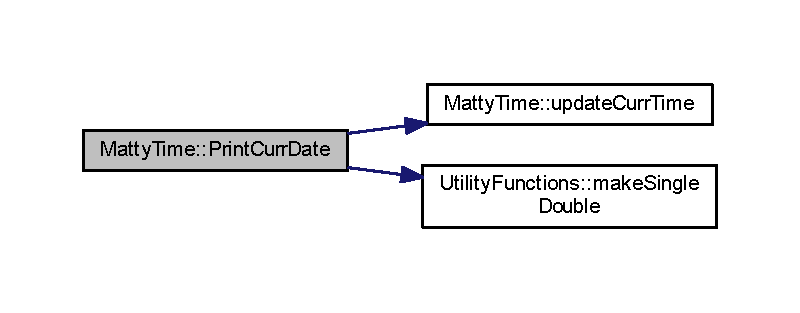
\includegraphics[width=350pt]{classMattyTime_af87198affde58c9f254dbf1601fb9f1e_cgraph}
\end{center}
\end{figure}
\hypertarget{classMattyTime_ac5ecfd2ff5329b3476906b39bbf02ae3}{}\label{classMattyTime_ac5ecfd2ff5329b3476906b39bbf02ae3} 
\index{Matty\+Time@{Matty\+Time}!Print\+Curr\+Time@{Print\+Curr\+Time}}
\index{Print\+Curr\+Time@{Print\+Curr\+Time}!Matty\+Time@{Matty\+Time}}
\subsubsection{\texorpdfstring{Print\+Curr\+Time()}{PrintCurrTime()}}
{\footnotesize\ttfamily Q\+String Matty\+Time\+::\+Print\+Curr\+Time (\begin{DoxyParamCaption}{ }\end{DoxyParamCaption})\hspace{0.3cm}{\ttfamily [static]}}



Definition at line 89 of file Matty\+Time.\+cpp.

Here is the call graph for this function\+:
\nopagebreak
\begin{figure}[H]
\begin{center}
\leavevmode
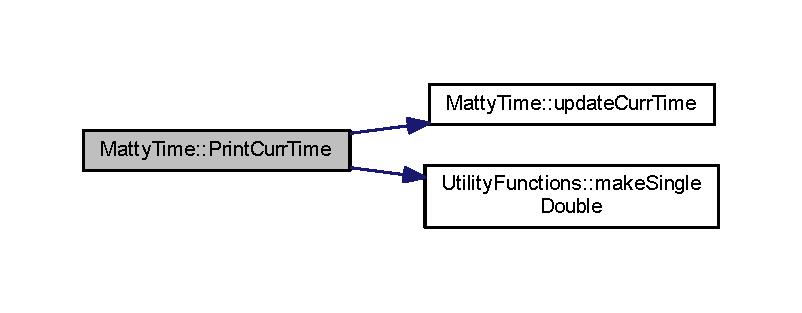
\includegraphics[width=350pt]{classMattyTime_ac5ecfd2ff5329b3476906b39bbf02ae3_cgraph}
\end{center}
\end{figure}
Here is the caller graph for this function\+:
\nopagebreak
\begin{figure}[H]
\begin{center}
\leavevmode
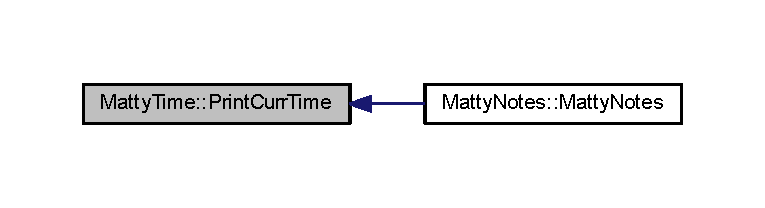
\includegraphics[width=350pt]{classMattyTime_ac5ecfd2ff5329b3476906b39bbf02ae3_icgraph}
\end{center}
\end{figure}
\hypertarget{classMattyTime_a96805256f90a469aa22824a1e2dd219d}{}\label{classMattyTime_a96805256f90a469aa22824a1e2dd219d} 
\index{Matty\+Time@{Matty\+Time}!Print\+Curr\+Time\+And\+Date@{Print\+Curr\+Time\+And\+Date}}
\index{Print\+Curr\+Time\+And\+Date@{Print\+Curr\+Time\+And\+Date}!Matty\+Time@{Matty\+Time}}
\subsubsection{\texorpdfstring{Print\+Curr\+Time\+And\+Date()}{PrintCurrTimeAndDate()}}
{\footnotesize\ttfamily Q\+String Matty\+Time\+::\+Print\+Curr\+Time\+And\+Date (\begin{DoxyParamCaption}{ }\end{DoxyParamCaption})\hspace{0.3cm}{\ttfamily [static]}}



Definition at line 119 of file Matty\+Time.\+cpp.

Here is the call graph for this function\+:
\nopagebreak
\begin{figure}[H]
\begin{center}
\leavevmode
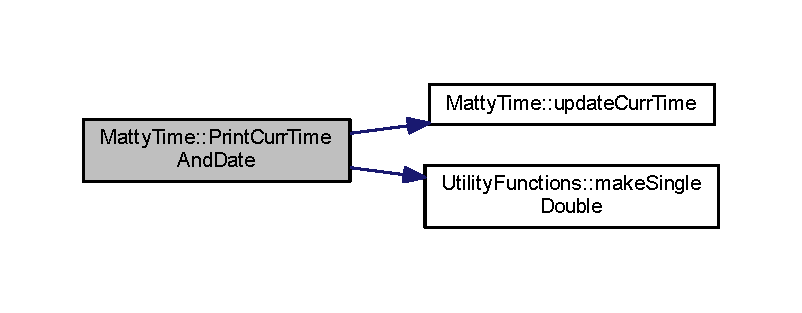
\includegraphics[width=350pt]{classMattyTime_a96805256f90a469aa22824a1e2dd219d_cgraph}
\end{center}
\end{figure}
\hypertarget{classMattyTime_a9d3500ad88197ee8e2db9f36aec1a266}{}\label{classMattyTime_a9d3500ad88197ee8e2db9f36aec1a266} 
\index{Matty\+Time@{Matty\+Time}!Print\+Curr\+Time\+Full@{Print\+Curr\+Time\+Full}}
\index{Print\+Curr\+Time\+Full@{Print\+Curr\+Time\+Full}!Matty\+Time@{Matty\+Time}}
\subsubsection{\texorpdfstring{Print\+Curr\+Time\+Full()}{PrintCurrTimeFull()}}
{\footnotesize\ttfamily Q\+String Matty\+Time\+::\+Print\+Curr\+Time\+Full (\begin{DoxyParamCaption}{ }\end{DoxyParamCaption})\hspace{0.3cm}{\ttfamily [static]}}



Definition at line 99 of file Matty\+Time.\+cpp.

Here is the call graph for this function\+:
\nopagebreak
\begin{figure}[H]
\begin{center}
\leavevmode
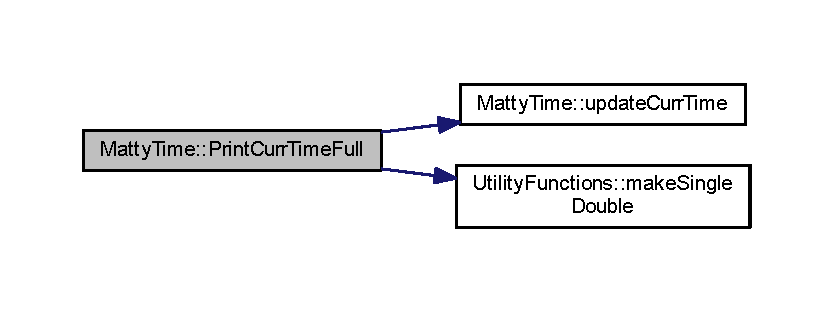
\includegraphics[width=350pt]{classMattyTime_a9d3500ad88197ee8e2db9f36aec1a266_cgraph}
\end{center}
\end{figure}
\hypertarget{classMattyTime_a82a6b06fa496b4d0f9b8d6e11d5b03c8}{}\label{classMattyTime_a82a6b06fa496b4d0f9b8d6e11d5b03c8} 
\index{Matty\+Time@{Matty\+Time}!Print\+Curr\+Time\+Full\+And\+Date@{Print\+Curr\+Time\+Full\+And\+Date}}
\index{Print\+Curr\+Time\+Full\+And\+Date@{Print\+Curr\+Time\+Full\+And\+Date}!Matty\+Time@{Matty\+Time}}
\subsubsection{\texorpdfstring{Print\+Curr\+Time\+Full\+And\+Date()}{PrintCurrTimeFullAndDate()}}
{\footnotesize\ttfamily Q\+String Matty\+Time\+::\+Print\+Curr\+Time\+Full\+And\+Date (\begin{DoxyParamCaption}{ }\end{DoxyParamCaption})\hspace{0.3cm}{\ttfamily [static]}}



Definition at line 131 of file Matty\+Time.\+cpp.

Here is the call graph for this function\+:
\nopagebreak
\begin{figure}[H]
\begin{center}
\leavevmode
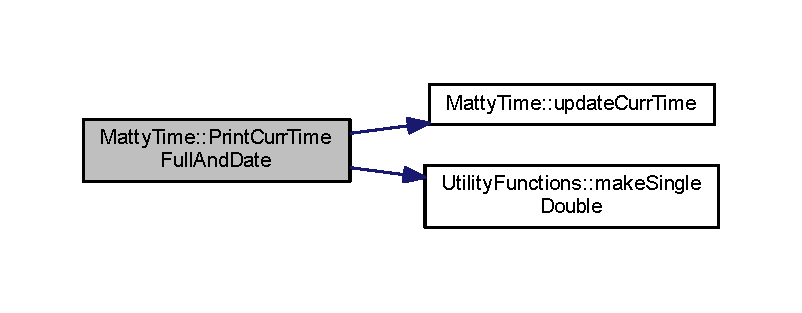
\includegraphics[width=350pt]{classMattyTime_a82a6b06fa496b4d0f9b8d6e11d5b03c8_cgraph}
\end{center}
\end{figure}
\hypertarget{classMattyTime_a646278576993d7ed05af67aee6ac96cb}{}\label{classMattyTime_a646278576993d7ed05af67aee6ac96cb} 
\index{Matty\+Time@{Matty\+Time}!Print\+User\+Date@{Print\+User\+Date}}
\index{Print\+User\+Date@{Print\+User\+Date}!Matty\+Time@{Matty\+Time}}
\subsubsection{\texorpdfstring{Print\+User\+Date()}{PrintUserDate()}}
{\footnotesize\ttfamily Q\+String Matty\+Time\+::\+Print\+User\+Date (\begin{DoxyParamCaption}{ }\end{DoxyParamCaption})}



Definition at line 163 of file Matty\+Time.\+cpp.

Here is the call graph for this function\+:
\nopagebreak
\begin{figure}[H]
\begin{center}
\leavevmode
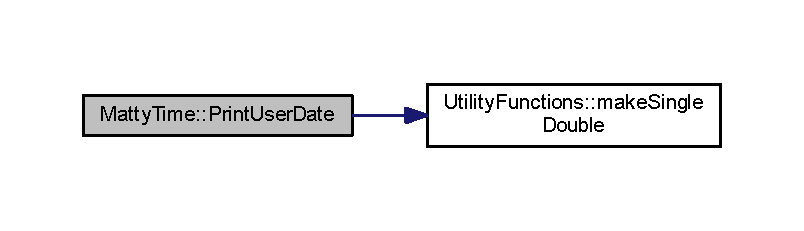
\includegraphics[width=350pt]{classMattyTime_a646278576993d7ed05af67aee6ac96cb_cgraph}
\end{center}
\end{figure}
Here is the caller graph for this function\+:
\nopagebreak
\begin{figure}[H]
\begin{center}
\leavevmode
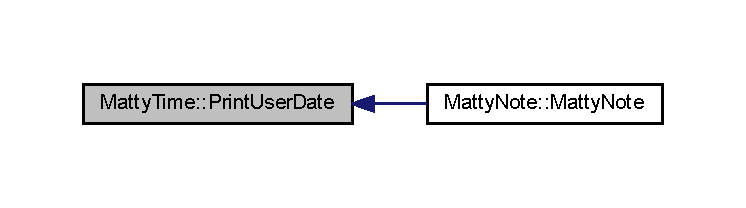
\includegraphics[width=350pt]{classMattyTime_a646278576993d7ed05af67aee6ac96cb_icgraph}
\end{center}
\end{figure}
\hypertarget{classMattyTime_a9cbf666ccbe45a8ca45f9ffc42d5102c}{}\label{classMattyTime_a9cbf666ccbe45a8ca45f9ffc42d5102c} 
\index{Matty\+Time@{Matty\+Time}!Print\+User\+Time@{Print\+User\+Time}}
\index{Print\+User\+Time@{Print\+User\+Time}!Matty\+Time@{Matty\+Time}}
\subsubsection{\texorpdfstring{Print\+User\+Time()}{PrintUserTime()}}
{\footnotesize\ttfamily Q\+String Matty\+Time\+::\+Print\+User\+Time (\begin{DoxyParamCaption}{ }\end{DoxyParamCaption})}



Definition at line 146 of file Matty\+Time.\+cpp.

Here is the call graph for this function\+:
\nopagebreak
\begin{figure}[H]
\begin{center}
\leavevmode
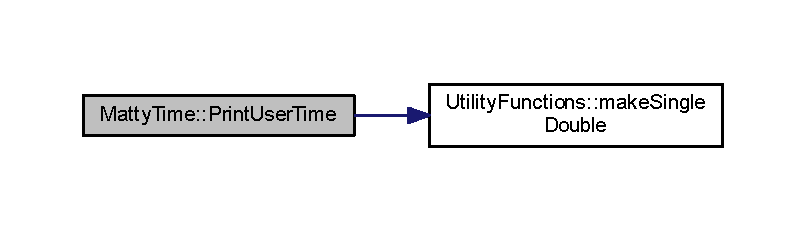
\includegraphics[width=350pt]{classMattyTime_a9cbf666ccbe45a8ca45f9ffc42d5102c_cgraph}
\end{center}
\end{figure}
Here is the caller graph for this function\+:
\nopagebreak
\begin{figure}[H]
\begin{center}
\leavevmode
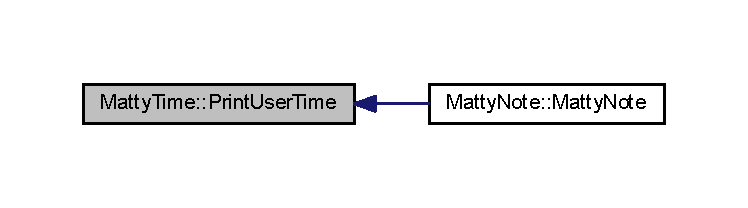
\includegraphics[width=350pt]{classMattyTime_a9cbf666ccbe45a8ca45f9ffc42d5102c_icgraph}
\end{center}
\end{figure}
\hypertarget{classMattyTime_afa30c1dd3bae1e8f50e816803f39d1c4}{}\label{classMattyTime_afa30c1dd3bae1e8f50e816803f39d1c4} 
\index{Matty\+Time@{Matty\+Time}!Print\+User\+Time\+And\+Date@{Print\+User\+Time\+And\+Date}}
\index{Print\+User\+Time\+And\+Date@{Print\+User\+Time\+And\+Date}!Matty\+Time@{Matty\+Time}}
\subsubsection{\texorpdfstring{Print\+User\+Time\+And\+Date()}{PrintUserTimeAndDate()}}
{\footnotesize\ttfamily Q\+String Matty\+Time\+::\+Print\+User\+Time\+And\+Date (\begin{DoxyParamCaption}{ }\end{DoxyParamCaption})}



Definition at line 172 of file Matty\+Time.\+cpp.

Here is the call graph for this function\+:
\nopagebreak
\begin{figure}[H]
\begin{center}
\leavevmode
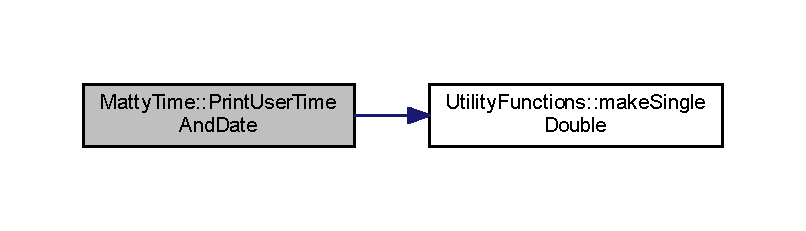
\includegraphics[width=350pt]{classMattyTime_afa30c1dd3bae1e8f50e816803f39d1c4_cgraph}
\end{center}
\end{figure}
\hypertarget{classMattyTime_a3fda0198071ebc95afe2d4405dd9c55e}{}\label{classMattyTime_a3fda0198071ebc95afe2d4405dd9c55e} 
\index{Matty\+Time@{Matty\+Time}!Print\+User\+Time\+Full@{Print\+User\+Time\+Full}}
\index{Print\+User\+Time\+Full@{Print\+User\+Time\+Full}!Matty\+Time@{Matty\+Time}}
\subsubsection{\texorpdfstring{Print\+User\+Time\+Full()}{PrintUserTimeFull()}}
{\footnotesize\ttfamily Q\+String Matty\+Time\+::\+Print\+User\+Time\+Full (\begin{DoxyParamCaption}{ }\end{DoxyParamCaption})}



Definition at line 154 of file Matty\+Time.\+cpp.

Here is the call graph for this function\+:
\nopagebreak
\begin{figure}[H]
\begin{center}
\leavevmode
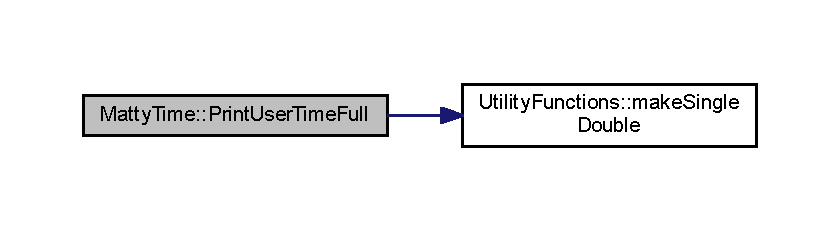
\includegraphics[width=350pt]{classMattyTime_a3fda0198071ebc95afe2d4405dd9c55e_cgraph}
\end{center}
\end{figure}
\hypertarget{classMattyTime_a6bcaa1f4975d99ab2f9025076de5ef99}{}\label{classMattyTime_a6bcaa1f4975d99ab2f9025076de5ef99} 
\index{Matty\+Time@{Matty\+Time}!Print\+User\+Time\+Full\+And\+Date@{Print\+User\+Time\+Full\+And\+Date}}
\index{Print\+User\+Time\+Full\+And\+Date@{Print\+User\+Time\+Full\+And\+Date}!Matty\+Time@{Matty\+Time}}
\subsubsection{\texorpdfstring{Print\+User\+Time\+Full\+And\+Date()}{PrintUserTimeFullAndDate()}}
{\footnotesize\ttfamily Q\+String Matty\+Time\+::\+Print\+User\+Time\+Full\+And\+Date (\begin{DoxyParamCaption}{ }\end{DoxyParamCaption})}



Definition at line 183 of file Matty\+Time.\+cpp.

Here is the call graph for this function\+:
\nopagebreak
\begin{figure}[H]
\begin{center}
\leavevmode
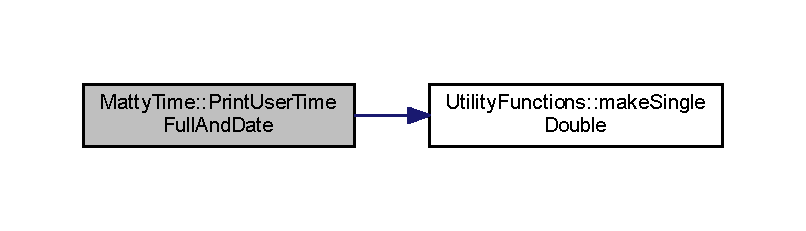
\includegraphics[width=350pt]{classMattyTime_a6bcaa1f4975d99ab2f9025076de5ef99_cgraph}
\end{center}
\end{figure}
\hypertarget{classMattyTime_a858357a5febc483c27f9bbf96b83b175}{}\label{classMattyTime_a858357a5febc483c27f9bbf96b83b175} 
\index{Matty\+Time@{Matty\+Time}!set\+User\+Date\+And\+Time@{set\+User\+Date\+And\+Time}}
\index{set\+User\+Date\+And\+Time@{set\+User\+Date\+And\+Time}!Matty\+Time@{Matty\+Time}}
\subsubsection{\texorpdfstring{set\+User\+Date\+And\+Time()}{setUserDateAndTime()}\hspace{0.1cm}{\footnotesize\ttfamily [1/5]}}
{\footnotesize\ttfamily void Matty\+Time\+::set\+User\+Date\+And\+Time (\begin{DoxyParamCaption}\item[{int}]{second }\end{DoxyParamCaption})}



Definition at line 47 of file Matty\+Time.\+cpp.

\hypertarget{classMattyTime_a60828ca950added6776f53ca3ea047fc}{}\label{classMattyTime_a60828ca950added6776f53ca3ea047fc} 
\index{Matty\+Time@{Matty\+Time}!set\+User\+Date\+And\+Time@{set\+User\+Date\+And\+Time}}
\index{set\+User\+Date\+And\+Time@{set\+User\+Date\+And\+Time}!Matty\+Time@{Matty\+Time}}
\subsubsection{\texorpdfstring{set\+User\+Date\+And\+Time()}{setUserDateAndTime()}\hspace{0.1cm}{\footnotesize\ttfamily [2/5]}}
{\footnotesize\ttfamily void Matty\+Time\+::set\+User\+Date\+And\+Time (\begin{DoxyParamCaption}\item[{int}]{hour,  }\item[{int}]{minute }\end{DoxyParamCaption})}



Definition at line 52 of file Matty\+Time.\+cpp.

\hypertarget{classMattyTime_ac6d00b726df1a8c493452dfc52332f6f}{}\label{classMattyTime_ac6d00b726df1a8c493452dfc52332f6f} 
\index{Matty\+Time@{Matty\+Time}!set\+User\+Date\+And\+Time@{set\+User\+Date\+And\+Time}}
\index{set\+User\+Date\+And\+Time@{set\+User\+Date\+And\+Time}!Matty\+Time@{Matty\+Time}}
\subsubsection{\texorpdfstring{set\+User\+Date\+And\+Time()}{setUserDateAndTime()}\hspace{0.1cm}{\footnotesize\ttfamily [3/5]}}
{\footnotesize\ttfamily void Matty\+Time\+::set\+User\+Date\+And\+Time (\begin{DoxyParamCaption}\item[{int}]{day,  }\item[{int}]{month,  }\item[{int}]{year }\end{DoxyParamCaption})}



Definition at line 59 of file Matty\+Time.\+cpp.

\hypertarget{classMattyTime_a34af1776506d7a99387db16982987e1c}{}\label{classMattyTime_a34af1776506d7a99387db16982987e1c} 
\index{Matty\+Time@{Matty\+Time}!set\+User\+Date\+And\+Time@{set\+User\+Date\+And\+Time}}
\index{set\+User\+Date\+And\+Time@{set\+User\+Date\+And\+Time}!Matty\+Time@{Matty\+Time}}
\subsubsection{\texorpdfstring{set\+User\+Date\+And\+Time()}{setUserDateAndTime()}\hspace{0.1cm}{\footnotesize\ttfamily [4/5]}}
{\footnotesize\ttfamily void Matty\+Time\+::set\+User\+Date\+And\+Time (\begin{DoxyParamCaption}\item[{int}]{hour,  }\item[{int}]{minute,  }\item[{int}]{day,  }\item[{int}]{month,  }\item[{int}]{year }\end{DoxyParamCaption})}



Definition at line 66 of file Matty\+Time.\+cpp.

\hypertarget{classMattyTime_ae470fb0341c517348ec3ea7d606f67c5}{}\label{classMattyTime_ae470fb0341c517348ec3ea7d606f67c5} 
\index{Matty\+Time@{Matty\+Time}!set\+User\+Date\+And\+Time@{set\+User\+Date\+And\+Time}}
\index{set\+User\+Date\+And\+Time@{set\+User\+Date\+And\+Time}!Matty\+Time@{Matty\+Time}}
\subsubsection{\texorpdfstring{set\+User\+Date\+And\+Time()}{setUserDateAndTime()}\hspace{0.1cm}{\footnotesize\ttfamily [5/5]}}
{\footnotesize\ttfamily void Matty\+Time\+::set\+User\+Date\+And\+Time (\begin{DoxyParamCaption}\item[{\hyperlink{structTimeAndDate}{Time\+And\+Date}}]{Time\+Date }\end{DoxyParamCaption})}



Definition at line 76 of file Matty\+Time.\+cpp.

\hypertarget{classMattyTime_a12b0e0b9c4d45248da89e2d4078d4d08}{}\label{classMattyTime_a12b0e0b9c4d45248da89e2d4078d4d08} 
\index{Matty\+Time@{Matty\+Time}!set\+User\+Day\+Of\+Week@{set\+User\+Day\+Of\+Week}}
\index{set\+User\+Day\+Of\+Week@{set\+User\+Day\+Of\+Week}!Matty\+Time@{Matty\+Time}}
\subsubsection{\texorpdfstring{set\+User\+Day\+Of\+Week()}{setUserDayOfWeek()}}
{\footnotesize\ttfamily void Matty\+Time\+::set\+User\+Day\+Of\+Week (\begin{DoxyParamCaption}{ }\end{DoxyParamCaption})}



Definition at line 210 of file Matty\+Time.\+cpp.

Here is the caller graph for this function\+:
\nopagebreak
\begin{figure}[H]
\begin{center}
\leavevmode
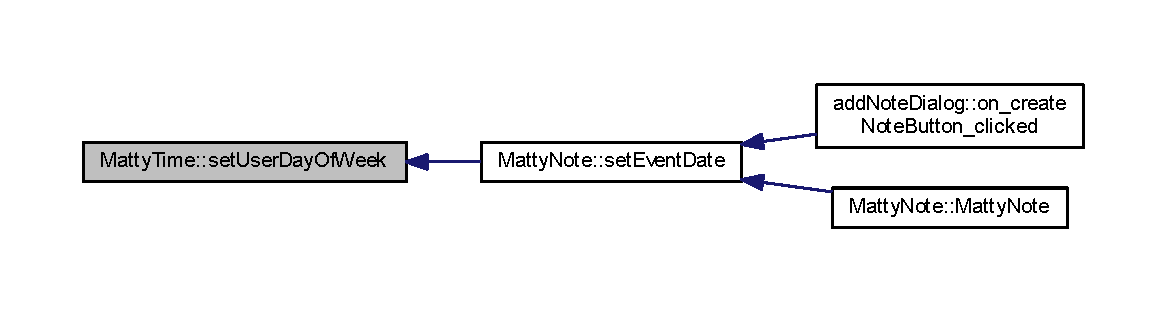
\includegraphics[width=350pt]{classMattyTime_a12b0e0b9c4d45248da89e2d4078d4d08_icgraph}
\end{center}
\end{figure}
\hypertarget{classMattyTime_afef585f71d11eed7777065af8ca0e9f0}{}\label{classMattyTime_afef585f71d11eed7777065af8ca0e9f0} 
\index{Matty\+Time@{Matty\+Time}!set\+User\+Time\+And\+Date\+Now@{set\+User\+Time\+And\+Date\+Now}}
\index{set\+User\+Time\+And\+Date\+Now@{set\+User\+Time\+And\+Date\+Now}!Matty\+Time@{Matty\+Time}}
\subsubsection{\texorpdfstring{set\+User\+Time\+And\+Date\+Now()}{setUserTimeAndDateNow()}}
{\footnotesize\ttfamily void Matty\+Time\+::set\+User\+Time\+And\+Date\+Now (\begin{DoxyParamCaption}{ }\end{DoxyParamCaption})}



Definition at line 195 of file Matty\+Time.\+cpp.

Here is the call graph for this function\+:
\nopagebreak
\begin{figure}[H]
\begin{center}
\leavevmode
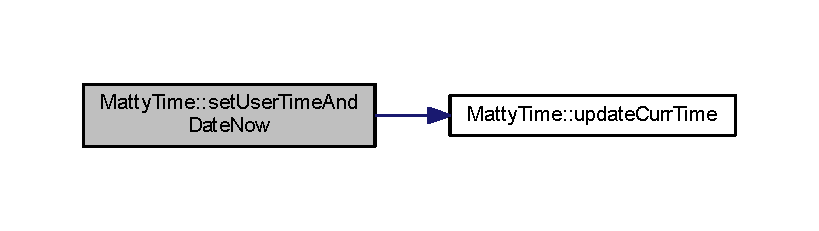
\includegraphics[width=350pt]{classMattyTime_afef585f71d11eed7777065af8ca0e9f0_cgraph}
\end{center}
\end{figure}
\hypertarget{classMattyTime_a6ae52c957bcf12e92624e09db890ce21}{}\label{classMattyTime_a6ae52c957bcf12e92624e09db890ce21} 
\index{Matty\+Time@{Matty\+Time}!set\+User\+Time\+And\+Date\+Null@{set\+User\+Time\+And\+Date\+Null}}
\index{set\+User\+Time\+And\+Date\+Null@{set\+User\+Time\+And\+Date\+Null}!Matty\+Time@{Matty\+Time}}
\subsubsection{\texorpdfstring{set\+User\+Time\+And\+Date\+Null()}{setUserTimeAndDateNull()}}
{\footnotesize\ttfamily void Matty\+Time\+::set\+User\+Time\+And\+Date\+Null (\begin{DoxyParamCaption}{ }\end{DoxyParamCaption})}



Definition at line 200 of file Matty\+Time.\+cpp.

Here is the caller graph for this function\+:
\nopagebreak
\begin{figure}[H]
\begin{center}
\leavevmode
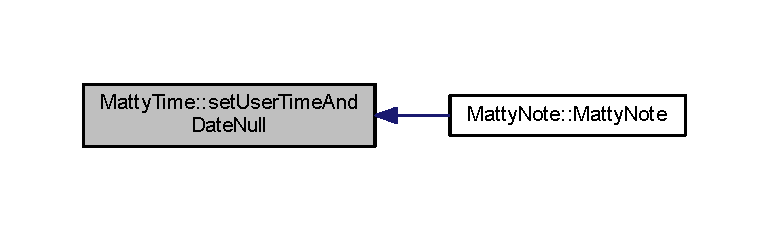
\includegraphics[width=350pt]{classMattyTime_a6ae52c957bcf12e92624e09db890ce21_icgraph}
\end{center}
\end{figure}
\hypertarget{classMattyTime_a52a7500e419fe56d10ddf2715fc96d06}{}\label{classMattyTime_a52a7500e419fe56d10ddf2715fc96d06} 
\index{Matty\+Time@{Matty\+Time}!update\+Curr\+Time@{update\+Curr\+Time}}
\index{update\+Curr\+Time@{update\+Curr\+Time}!Matty\+Time@{Matty\+Time}}
\subsubsection{\texorpdfstring{update\+Curr\+Time()}{updateCurrTime()}}
{\footnotesize\ttfamily void Matty\+Time\+::update\+Curr\+Time (\begin{DoxyParamCaption}{ }\end{DoxyParamCaption})\hspace{0.3cm}{\ttfamily [static]}}



Definition at line 27 of file Matty\+Time.\+cpp.

Here is the caller graph for this function\+:
\nopagebreak
\begin{figure}[H]
\begin{center}
\leavevmode
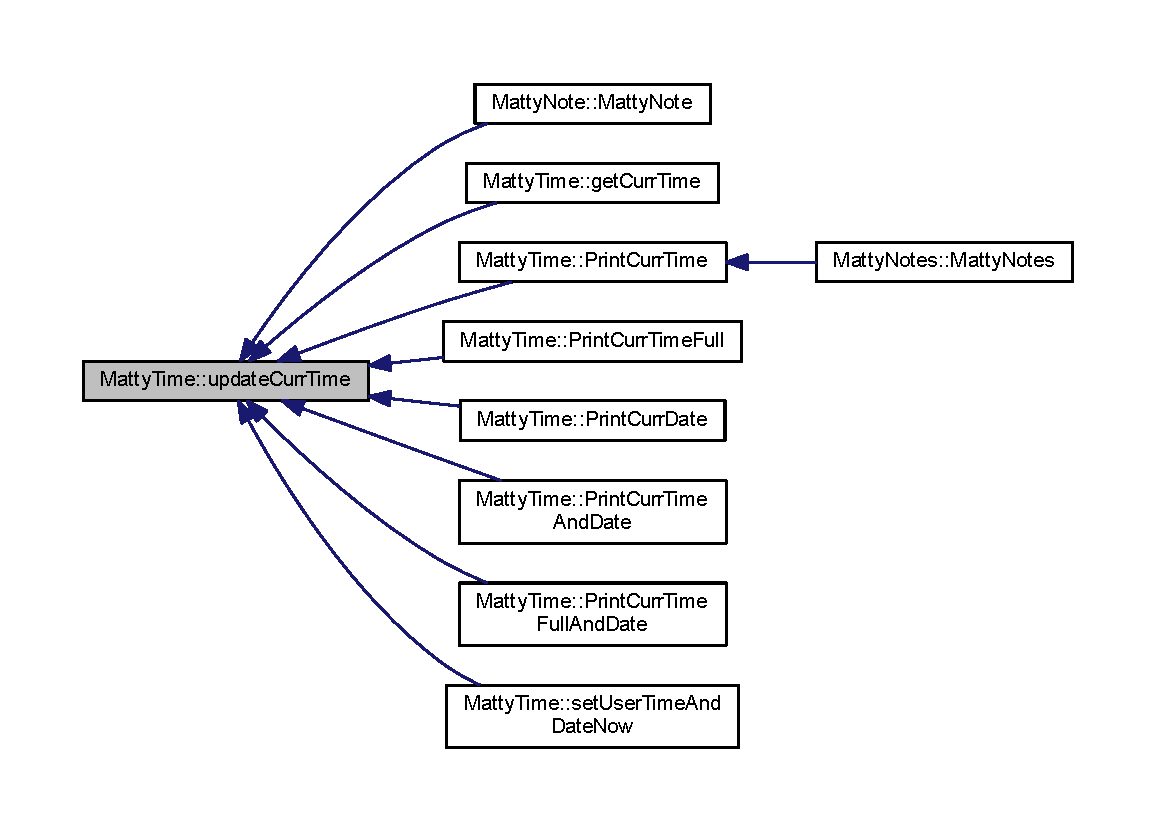
\includegraphics[width=350pt]{classMattyTime_a52a7500e419fe56d10ddf2715fc96d06_icgraph}
\end{center}
\end{figure}


\subsection{Member Data Documentation}
\hypertarget{classMattyTime_a458337456f43243073ae78976e86618f}{}\label{classMattyTime_a458337456f43243073ae78976e86618f} 
\index{Matty\+Time@{Matty\+Time}!Curr\+Time@{Curr\+Time}}
\index{Curr\+Time@{Curr\+Time}!Matty\+Time@{Matty\+Time}}
\subsubsection{\texorpdfstring{Curr\+Time}{CurrTime}}
{\footnotesize\ttfamily \hyperlink{structTimeAndDate}{Time\+And\+Date} Matty\+Time\+::\+Curr\+Time\hspace{0.3cm}{\ttfamily [static]}}



Definition at line 39 of file Matty\+Time.\+h.

\hypertarget{classMattyTime_a7a1ceab576011e56405b49d7bd81e475}{}\label{classMattyTime_a7a1ceab576011e56405b49d7bd81e475} 
\index{Matty\+Time@{Matty\+Time}!User\+Time\+And\+Date@{User\+Time\+And\+Date}}
\index{User\+Time\+And\+Date@{User\+Time\+And\+Date}!Matty\+Time@{Matty\+Time}}
\subsubsection{\texorpdfstring{User\+Time\+And\+Date}{UserTimeAndDate}}
{\footnotesize\ttfamily \hyperlink{structTimeAndDate}{Time\+And\+Date} Matty\+Time\+::\+User\+Time\+And\+Date}



Definition at line 40 of file Matty\+Time.\+h.



The documentation for this class was generated from the following files\+:\begin{DoxyCompactItemize}
\item 
C\+:/\+Users/\+Ogrigorieva/\+Visual Studio 2015/\+Projects/\+Personal/\+Matty\+Notes/\hyperlink{MattyTime_8h}{Matty\+Time.\+h}\item 
C\+:/\+Users/\+Ogrigorieva/\+Visual Studio 2015/\+Projects/\+Personal/\+Matty\+Notes/\hyperlink{MattyTime_8cpp}{Matty\+Time.\+cpp}\end{DoxyCompactItemize}

\hypertarget{classNoteHolder}{}\section{Note\+Holder Class Reference}
\label{classNoteHolder}\index{Note\+Holder@{Note\+Holder}}


{\ttfamily \#include $<$Note\+Holder.\+h$>$}

\subsection*{Public Member Functions}
\begin{DoxyCompactItemize}
\item 
\hyperlink{classNoteHolder_a8a6d0e272ccfe8f56534c646b8c5e92c}{Note\+Holder} ()
\item 
\hyperlink{classNoteHolder_afaeb3c127fbbc30d03b69e2cb0f15f2a}{$\sim$\+Note\+Holder} ()
\end{DoxyCompactItemize}
\subsection*{Static Public Member Functions}
\begin{DoxyCompactItemize}
\item 
static Q\+Vector$<$ class \hyperlink{classMattyNote}{Matty\+Note} $>$ \hyperlink{classNoteHolder_ab52d375cf5ab24f0512fab6308ec8b25}{sort\+Notes\+By\+Cr\+Date} ()
\item 
static void \hyperlink{classNoteHolder_a9fbdbdf5cc2628f360c45eb861eacded}{show\+Notes} (int order\+Direction, Q\+V\+Box\+Layout $\ast$Parent\+Layout)
\end{DoxyCompactItemize}
\subsection*{Static Private Attributes}
\begin{DoxyCompactItemize}
\item 
static int \hyperlink{classNoteHolder_a7fd3dd17b879e12cef0b0466ef04ed37}{Note\+Count} = 0
\item 
static Q\+Vector$<$ class \hyperlink{classMattyNote}{Matty\+Note} $>$ \hyperlink{classNoteHolder_a00b2d3ea1a95febaf0d8a5526b786e95}{List\+Of\+Notes} = Q\+Vector$<$class \hyperlink{classMattyNote}{Matty\+Note}$>$()
\item 
static Q\+Vector$<$ Q\+String $>$ \hyperlink{classNoteHolder_a9106819d414e3e131560ef3fcbea4d18}{List\+Of\+Group\+Boxe\+Names} = Q\+Vector$<$Q\+String$>$()
\end{DoxyCompactItemize}


\subsection{Detailed Description}


Definition at line 10 of file Note\+Holder.\+h.



\subsection{Constructor \& Destructor Documentation}
\hypertarget{classNoteHolder_a8a6d0e272ccfe8f56534c646b8c5e92c}{}\label{classNoteHolder_a8a6d0e272ccfe8f56534c646b8c5e92c} 
\index{Note\+Holder@{Note\+Holder}!Note\+Holder@{Note\+Holder}}
\index{Note\+Holder@{Note\+Holder}!Note\+Holder@{Note\+Holder}}
\subsubsection{\texorpdfstring{Note\+Holder()}{NoteHolder()}}
{\footnotesize\ttfamily Note\+Holder\+::\+Note\+Holder (\begin{DoxyParamCaption}{ }\end{DoxyParamCaption})}



Definition at line 12 of file Note\+Holder.\+cpp.

\hypertarget{classNoteHolder_afaeb3c127fbbc30d03b69e2cb0f15f2a}{}\label{classNoteHolder_afaeb3c127fbbc30d03b69e2cb0f15f2a} 
\index{Note\+Holder@{Note\+Holder}!````~Note\+Holder@{$\sim$\+Note\+Holder}}
\index{````~Note\+Holder@{$\sim$\+Note\+Holder}!Note\+Holder@{Note\+Holder}}
\subsubsection{\texorpdfstring{$\sim$\+Note\+Holder()}{~NoteHolder()}}
{\footnotesize\ttfamily Note\+Holder\+::$\sim$\+Note\+Holder (\begin{DoxyParamCaption}{ }\end{DoxyParamCaption})}



Definition at line 17 of file Note\+Holder.\+cpp.



\subsection{Member Function Documentation}
\hypertarget{classNoteHolder_a9fbdbdf5cc2628f360c45eb861eacded}{}\label{classNoteHolder_a9fbdbdf5cc2628f360c45eb861eacded} 
\index{Note\+Holder@{Note\+Holder}!show\+Notes@{show\+Notes}}
\index{show\+Notes@{show\+Notes}!Note\+Holder@{Note\+Holder}}
\subsubsection{\texorpdfstring{show\+Notes()}{showNotes()}}
{\footnotesize\ttfamily void Note\+Holder\+::show\+Notes (\begin{DoxyParamCaption}\item[{int}]{order\+Direction,  }\item[{Q\+V\+Box\+Layout $\ast$}]{Parent\+Layout }\end{DoxyParamCaption})\hspace{0.3cm}{\ttfamily [static]}}



Definition at line 40 of file Note\+Holder.\+cpp.

Here is the call graph for this function\+:
\nopagebreak
\begin{figure}[H]
\begin{center}
\leavevmode
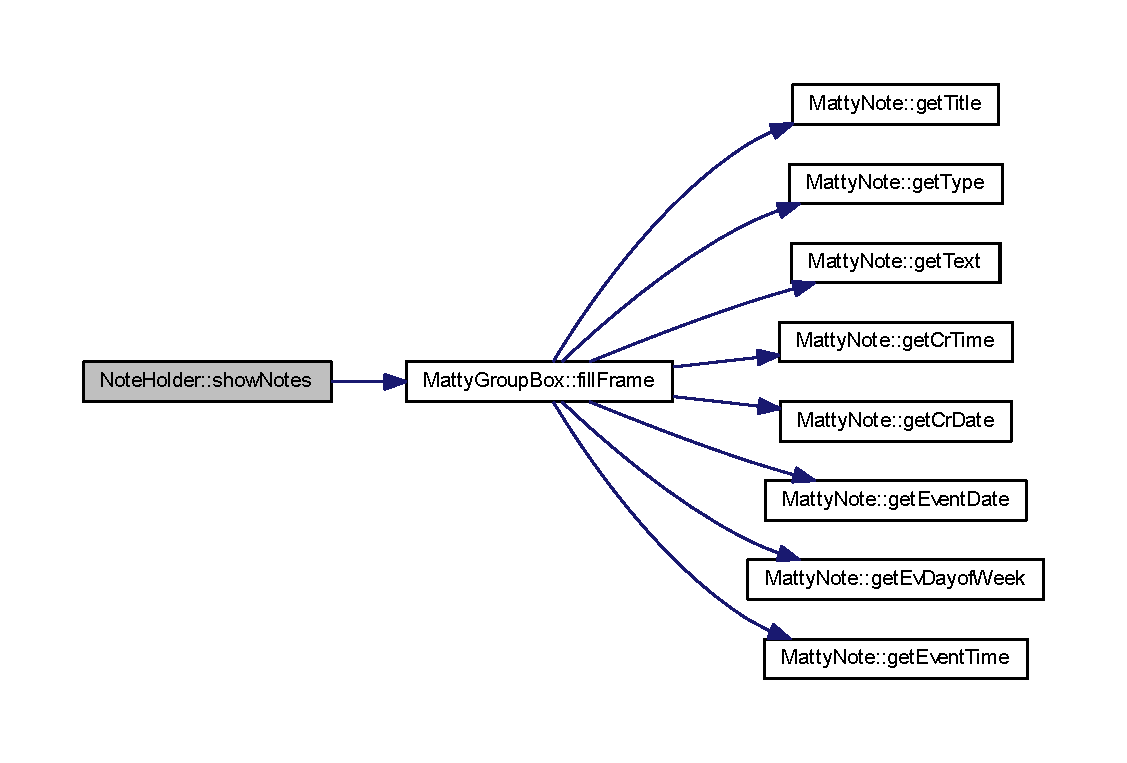
\includegraphics[width=350pt]{classNoteHolder_a9fbdbdf5cc2628f360c45eb861eacded_cgraph}
\end{center}
\end{figure}
Here is the caller graph for this function\+:
\nopagebreak
\begin{figure}[H]
\begin{center}
\leavevmode
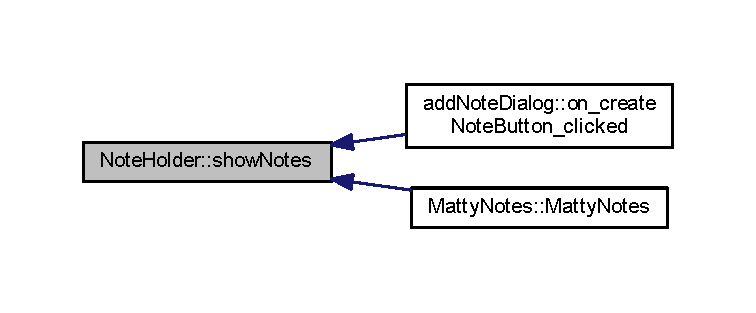
\includegraphics[width=350pt]{classNoteHolder_a9fbdbdf5cc2628f360c45eb861eacded_icgraph}
\end{center}
\end{figure}
\hypertarget{classNoteHolder_ab52d375cf5ab24f0512fab6308ec8b25}{}\label{classNoteHolder_ab52d375cf5ab24f0512fab6308ec8b25} 
\index{Note\+Holder@{Note\+Holder}!sort\+Notes\+By\+Cr\+Date@{sort\+Notes\+By\+Cr\+Date}}
\index{sort\+Notes\+By\+Cr\+Date@{sort\+Notes\+By\+Cr\+Date}!Note\+Holder@{Note\+Holder}}
\subsubsection{\texorpdfstring{sort\+Notes\+By\+Cr\+Date()}{sortNotesByCrDate()}}
{\footnotesize\ttfamily Q\+Vector$<$ class \hyperlink{classMattyNote}{Matty\+Note} $>$ Note\+Holder\+::sort\+Notes\+By\+Cr\+Date (\begin{DoxyParamCaption}{ }\end{DoxyParamCaption})\hspace{0.3cm}{\ttfamily [static]}}



Definition at line 21 of file Note\+Holder.\+cpp.

Here is the call graph for this function\+:
\nopagebreak
\begin{figure}[H]
\begin{center}
\leavevmode
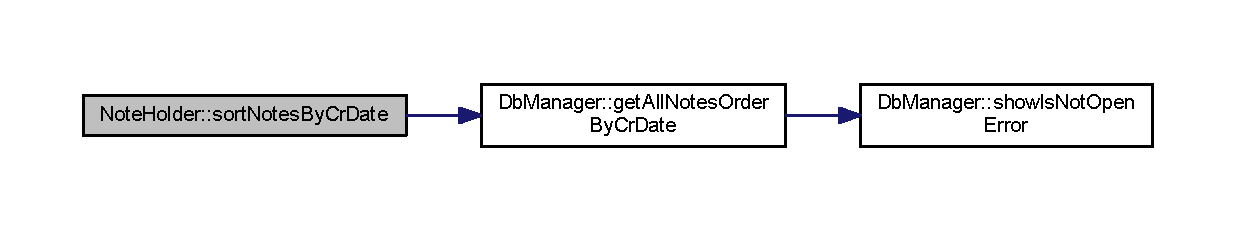
\includegraphics[width=350pt]{classNoteHolder_ab52d375cf5ab24f0512fab6308ec8b25_cgraph}
\end{center}
\end{figure}
Here is the caller graph for this function\+:
\nopagebreak
\begin{figure}[H]
\begin{center}
\leavevmode
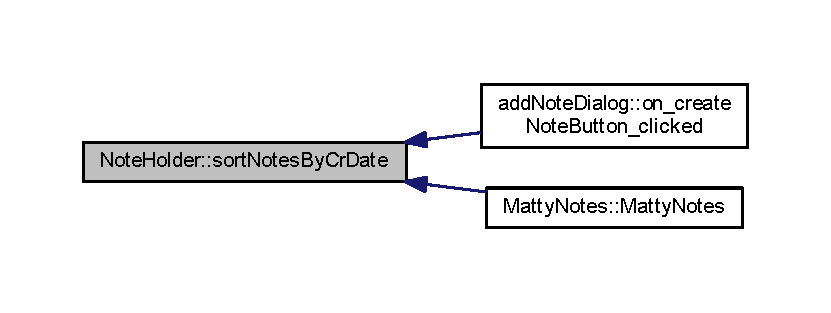
\includegraphics[width=350pt]{classNoteHolder_ab52d375cf5ab24f0512fab6308ec8b25_icgraph}
\end{center}
\end{figure}


\subsection{Member Data Documentation}
\hypertarget{classNoteHolder_a9106819d414e3e131560ef3fcbea4d18}{}\label{classNoteHolder_a9106819d414e3e131560ef3fcbea4d18} 
\index{Note\+Holder@{Note\+Holder}!List\+Of\+Group\+Boxe\+Names@{List\+Of\+Group\+Boxe\+Names}}
\index{List\+Of\+Group\+Boxe\+Names@{List\+Of\+Group\+Boxe\+Names}!Note\+Holder@{Note\+Holder}}
\subsubsection{\texorpdfstring{List\+Of\+Group\+Boxe\+Names}{ListOfGroupBoxeNames}}
{\footnotesize\ttfamily Q\+Vector$<$ Q\+String $>$ Note\+Holder\+::\+List\+Of\+Group\+Boxe\+Names = Q\+Vector$<$Q\+String$>$()\hspace{0.3cm}{\ttfamily [static]}, {\ttfamily [private]}}



Definition at line 20 of file Note\+Holder.\+h.

\hypertarget{classNoteHolder_a00b2d3ea1a95febaf0d8a5526b786e95}{}\label{classNoteHolder_a00b2d3ea1a95febaf0d8a5526b786e95} 
\index{Note\+Holder@{Note\+Holder}!List\+Of\+Notes@{List\+Of\+Notes}}
\index{List\+Of\+Notes@{List\+Of\+Notes}!Note\+Holder@{Note\+Holder}}
\subsubsection{\texorpdfstring{List\+Of\+Notes}{ListOfNotes}}
{\footnotesize\ttfamily Q\+Vector$<$ class \hyperlink{classMattyNote}{Matty\+Note} $>$ Note\+Holder\+::\+List\+Of\+Notes = Q\+Vector$<$class \hyperlink{classMattyNote}{Matty\+Note}$>$()\hspace{0.3cm}{\ttfamily [static]}, {\ttfamily [private]}}



Definition at line 19 of file Note\+Holder.\+h.

\hypertarget{classNoteHolder_a7fd3dd17b879e12cef0b0466ef04ed37}{}\label{classNoteHolder_a7fd3dd17b879e12cef0b0466ef04ed37} 
\index{Note\+Holder@{Note\+Holder}!Note\+Count@{Note\+Count}}
\index{Note\+Count@{Note\+Count}!Note\+Holder@{Note\+Holder}}
\subsubsection{\texorpdfstring{Note\+Count}{NoteCount}}
{\footnotesize\ttfamily int Note\+Holder\+::\+Note\+Count = 0\hspace{0.3cm}{\ttfamily [static]}, {\ttfamily [private]}}



Definition at line 18 of file Note\+Holder.\+h.



The documentation for this class was generated from the following files\+:\begin{DoxyCompactItemize}
\item 
C\+:/\+Users/\+Ogrigorieva/\+Visual Studio 2015/\+Projects/\+Personal/\+Matty\+Notes/\hyperlink{NoteHolder_8h}{Note\+Holder.\+h}\item 
C\+:/\+Users/\+Ogrigorieva/\+Visual Studio 2015/\+Projects/\+Personal/\+Matty\+Notes/\hyperlink{NoteHolder_8cpp}{Note\+Holder.\+cpp}\end{DoxyCompactItemize}

\hypertarget{structqt__meta__stringdata__addNoteDialog__t}{}\section{qt\+\_\+meta\+\_\+stringdata\+\_\+add\+Note\+Dialog\+\_\+t Struct Reference}
\label{structqt__meta__stringdata__addNoteDialog__t}\index{qt\+\_\+meta\+\_\+stringdata\+\_\+add\+Note\+Dialog\+\_\+t@{qt\+\_\+meta\+\_\+stringdata\+\_\+add\+Note\+Dialog\+\_\+t}}
\subsection*{Public Attributes}
\begin{DoxyCompactItemize}
\item 
Q\+Byte\+Array\+Data \hyperlink{structqt__meta__stringdata__addNoteDialog__t_a6182404ea668458da8f435aaa45fa4ec}{data} \mbox{[}4\mbox{]}
\item 
char \hyperlink{structqt__meta__stringdata__addNoteDialog__t_aa36bd0528981067f754981fb90d385d8}{stringdata0} \mbox{[}77\mbox{]}
\end{DoxyCompactItemize}


\subsection{Detailed Description}


Definition at line 22 of file moc\+\_\+addnotedialog.\+cpp.



\subsection{Member Data Documentation}
\hypertarget{structqt__meta__stringdata__addNoteDialog__t_a6182404ea668458da8f435aaa45fa4ec}{}\label{structqt__meta__stringdata__addNoteDialog__t_a6182404ea668458da8f435aaa45fa4ec} 
\index{qt\+\_\+meta\+\_\+stringdata\+\_\+add\+Note\+Dialog\+\_\+t@{qt\+\_\+meta\+\_\+stringdata\+\_\+add\+Note\+Dialog\+\_\+t}!data@{data}}
\index{data@{data}!qt\+\_\+meta\+\_\+stringdata\+\_\+add\+Note\+Dialog\+\_\+t@{qt\+\_\+meta\+\_\+stringdata\+\_\+add\+Note\+Dialog\+\_\+t}}
\subsubsection{\texorpdfstring{data}{data}}
{\footnotesize\ttfamily Q\+Byte\+Array\+Data qt\+\_\+meta\+\_\+stringdata\+\_\+add\+Note\+Dialog\+\_\+t\+::data}



Definition at line 23 of file moc\+\_\+addnotedialog.\+cpp.

\hypertarget{structqt__meta__stringdata__addNoteDialog__t_aa36bd0528981067f754981fb90d385d8}{}\label{structqt__meta__stringdata__addNoteDialog__t_aa36bd0528981067f754981fb90d385d8} 
\index{qt\+\_\+meta\+\_\+stringdata\+\_\+add\+Note\+Dialog\+\_\+t@{qt\+\_\+meta\+\_\+stringdata\+\_\+add\+Note\+Dialog\+\_\+t}!stringdata0@{stringdata0}}
\index{stringdata0@{stringdata0}!qt\+\_\+meta\+\_\+stringdata\+\_\+add\+Note\+Dialog\+\_\+t@{qt\+\_\+meta\+\_\+stringdata\+\_\+add\+Note\+Dialog\+\_\+t}}
\subsubsection{\texorpdfstring{stringdata0}{stringdata0}}
{\footnotesize\ttfamily char qt\+\_\+meta\+\_\+stringdata\+\_\+add\+Note\+Dialog\+\_\+t\+::stringdata0}



Definition at line 24 of file moc\+\_\+addnotedialog.\+cpp.



The documentation for this struct was generated from the following file\+:\begin{DoxyCompactItemize}
\item 
C\+:/\+Users/\+Ogrigorieva/\+Visual Studio 2015/\+Projects/\+Personal/\+Matty\+Notes/\+Generated\+Files/\+Debug/\hyperlink{Debug_2moc__addnotedialog_8cpp}{moc\+\_\+addnotedialog.\+cpp}\end{DoxyCompactItemize}

\hypertarget{structqt__meta__stringdata__MattyGroupBox__t}{}\section{qt\+\_\+meta\+\_\+stringdata\+\_\+\+Matty\+Group\+Box\+\_\+t Struct Reference}
\label{structqt__meta__stringdata__MattyGroupBox__t}\index{qt\+\_\+meta\+\_\+stringdata\+\_\+\+Matty\+Group\+Box\+\_\+t@{qt\+\_\+meta\+\_\+stringdata\+\_\+\+Matty\+Group\+Box\+\_\+t}}
\subsection*{Public Attributes}
\begin{DoxyCompactItemize}
\item 
Q\+Byte\+Array\+Data \hyperlink{structqt__meta__stringdata__MattyGroupBox__t_a4f9861808bbbbbe2e28aeb88748e1839}{data} \mbox{[}3\mbox{]}
\item 
char \hyperlink{structqt__meta__stringdata__MattyGroupBox__t_a7dd92394a2028cd695441f73c63474c9}{stringdata0} \mbox{[}26\mbox{]}
\end{DoxyCompactItemize}


\subsection{Detailed Description}


Definition at line 22 of file moc\+\_\+\+Matty\+Group\+Box.\+cpp.



\subsection{Member Data Documentation}
\hypertarget{structqt__meta__stringdata__MattyGroupBox__t_a4f9861808bbbbbe2e28aeb88748e1839}{}\label{structqt__meta__stringdata__MattyGroupBox__t_a4f9861808bbbbbe2e28aeb88748e1839} 
\index{qt\+\_\+meta\+\_\+stringdata\+\_\+\+Matty\+Group\+Box\+\_\+t@{qt\+\_\+meta\+\_\+stringdata\+\_\+\+Matty\+Group\+Box\+\_\+t}!data@{data}}
\index{data@{data}!qt\+\_\+meta\+\_\+stringdata\+\_\+\+Matty\+Group\+Box\+\_\+t@{qt\+\_\+meta\+\_\+stringdata\+\_\+\+Matty\+Group\+Box\+\_\+t}}
\subsubsection{\texorpdfstring{data}{data}}
{\footnotesize\ttfamily Q\+Byte\+Array\+Data qt\+\_\+meta\+\_\+stringdata\+\_\+\+Matty\+Group\+Box\+\_\+t\+::data}



Definition at line 23 of file moc\+\_\+\+Matty\+Group\+Box.\+cpp.

\hypertarget{structqt__meta__stringdata__MattyGroupBox__t_a7dd92394a2028cd695441f73c63474c9}{}\label{structqt__meta__stringdata__MattyGroupBox__t_a7dd92394a2028cd695441f73c63474c9} 
\index{qt\+\_\+meta\+\_\+stringdata\+\_\+\+Matty\+Group\+Box\+\_\+t@{qt\+\_\+meta\+\_\+stringdata\+\_\+\+Matty\+Group\+Box\+\_\+t}!stringdata0@{stringdata0}}
\index{stringdata0@{stringdata0}!qt\+\_\+meta\+\_\+stringdata\+\_\+\+Matty\+Group\+Box\+\_\+t@{qt\+\_\+meta\+\_\+stringdata\+\_\+\+Matty\+Group\+Box\+\_\+t}}
\subsubsection{\texorpdfstring{stringdata0}{stringdata0}}
{\footnotesize\ttfamily char qt\+\_\+meta\+\_\+stringdata\+\_\+\+Matty\+Group\+Box\+\_\+t\+::stringdata0}



Definition at line 24 of file moc\+\_\+\+Matty\+Group\+Box.\+cpp.



The documentation for this struct was generated from the following file\+:\begin{DoxyCompactItemize}
\item 
C\+:/\+Users/\+Ogrigorieva/\+Visual Studio 2015/\+Projects/\+Personal/\+Matty\+Notes/\+Generated\+Files/\+Debug/\hyperlink{Debug_2moc__MattyGroupBox_8cpp}{moc\+\_\+\+Matty\+Group\+Box.\+cpp}\end{DoxyCompactItemize}

\hypertarget{structqt__meta__stringdata__MattyNotes__t}{}\section{qt\+\_\+meta\+\_\+stringdata\+\_\+\+Matty\+Notes\+\_\+t Struct Reference}
\label{structqt__meta__stringdata__MattyNotes__t}\index{qt\+\_\+meta\+\_\+stringdata\+\_\+\+Matty\+Notes\+\_\+t@{qt\+\_\+meta\+\_\+stringdata\+\_\+\+Matty\+Notes\+\_\+t}}
\subsection*{Public Attributes}
\begin{DoxyCompactItemize}
\item 
Q\+Byte\+Array\+Data \hyperlink{structqt__meta__stringdata__MattyNotes__t_a9dc2d4f6359a5999afbd08eda36eed8f}{data} \mbox{[}6\mbox{]}
\item 
char \hyperlink{structqt__meta__stringdata__MattyNotes__t_aefec099c932333985b581afe6840c1d4}{stringdata0} \mbox{[}83\mbox{]}
\end{DoxyCompactItemize}


\subsection{Detailed Description}


Definition at line 22 of file moc\+\_\+mattynotes.\+cpp.



\subsection{Member Data Documentation}
\hypertarget{structqt__meta__stringdata__MattyNotes__t_a9dc2d4f6359a5999afbd08eda36eed8f}{}\label{structqt__meta__stringdata__MattyNotes__t_a9dc2d4f6359a5999afbd08eda36eed8f} 
\index{qt\+\_\+meta\+\_\+stringdata\+\_\+\+Matty\+Notes\+\_\+t@{qt\+\_\+meta\+\_\+stringdata\+\_\+\+Matty\+Notes\+\_\+t}!data@{data}}
\index{data@{data}!qt\+\_\+meta\+\_\+stringdata\+\_\+\+Matty\+Notes\+\_\+t@{qt\+\_\+meta\+\_\+stringdata\+\_\+\+Matty\+Notes\+\_\+t}}
\subsubsection{\texorpdfstring{data}{data}}
{\footnotesize\ttfamily Q\+Byte\+Array\+Data qt\+\_\+meta\+\_\+stringdata\+\_\+\+Matty\+Notes\+\_\+t\+::data}



Definition at line 23 of file moc\+\_\+mattynotes.\+cpp.

\hypertarget{structqt__meta__stringdata__MattyNotes__t_aefec099c932333985b581afe6840c1d4}{}\label{structqt__meta__stringdata__MattyNotes__t_aefec099c932333985b581afe6840c1d4} 
\index{qt\+\_\+meta\+\_\+stringdata\+\_\+\+Matty\+Notes\+\_\+t@{qt\+\_\+meta\+\_\+stringdata\+\_\+\+Matty\+Notes\+\_\+t}!stringdata0@{stringdata0}}
\index{stringdata0@{stringdata0}!qt\+\_\+meta\+\_\+stringdata\+\_\+\+Matty\+Notes\+\_\+t@{qt\+\_\+meta\+\_\+stringdata\+\_\+\+Matty\+Notes\+\_\+t}}
\subsubsection{\texorpdfstring{stringdata0}{stringdata0}}
{\footnotesize\ttfamily char qt\+\_\+meta\+\_\+stringdata\+\_\+\+Matty\+Notes\+\_\+t\+::stringdata0}



Definition at line 24 of file moc\+\_\+mattynotes.\+cpp.



The documentation for this struct was generated from the following file\+:\begin{DoxyCompactItemize}
\item 
C\+:/\+Users/\+Ogrigorieva/\+Visual Studio 2015/\+Projects/\+Personal/\+Matty\+Notes/\+Generated\+Files/\+Debug/\hyperlink{Debug_2moc__mattynotes_8cpp}{moc\+\_\+mattynotes.\+cpp}\end{DoxyCompactItemize}

\hypertarget{structqt__meta__stringdata__MattySettings__t}{}\section{qt\+\_\+meta\+\_\+stringdata\+\_\+\+Matty\+Settings\+\_\+t Struct Reference}
\label{structqt__meta__stringdata__MattySettings__t}\index{qt\+\_\+meta\+\_\+stringdata\+\_\+\+Matty\+Settings\+\_\+t@{qt\+\_\+meta\+\_\+stringdata\+\_\+\+Matty\+Settings\+\_\+t}}
\subsection*{Public Attributes}
\begin{DoxyCompactItemize}
\item 
Q\+Byte\+Array\+Data \hyperlink{structqt__meta__stringdata__MattySettings__t_aecbfa5782c64051df47fbe5036e76fa8}{data} \mbox{[}1\mbox{]}
\item 
char \hyperlink{structqt__meta__stringdata__MattySettings__t_a266b7703ec9f21f50b222ad586c210e3}{stringdata0} \mbox{[}14\mbox{]}
\end{DoxyCompactItemize}


\subsection{Detailed Description}


Definition at line 22 of file moc\+\_\+mattysettings.\+cpp.



\subsection{Member Data Documentation}
\hypertarget{structqt__meta__stringdata__MattySettings__t_aecbfa5782c64051df47fbe5036e76fa8}{}\label{structqt__meta__stringdata__MattySettings__t_aecbfa5782c64051df47fbe5036e76fa8} 
\index{qt\+\_\+meta\+\_\+stringdata\+\_\+\+Matty\+Settings\+\_\+t@{qt\+\_\+meta\+\_\+stringdata\+\_\+\+Matty\+Settings\+\_\+t}!data@{data}}
\index{data@{data}!qt\+\_\+meta\+\_\+stringdata\+\_\+\+Matty\+Settings\+\_\+t@{qt\+\_\+meta\+\_\+stringdata\+\_\+\+Matty\+Settings\+\_\+t}}
\subsubsection{\texorpdfstring{data}{data}}
{\footnotesize\ttfamily Q\+Byte\+Array\+Data qt\+\_\+meta\+\_\+stringdata\+\_\+\+Matty\+Settings\+\_\+t\+::data}



Definition at line 23 of file moc\+\_\+mattysettings.\+cpp.

\hypertarget{structqt__meta__stringdata__MattySettings__t_a266b7703ec9f21f50b222ad586c210e3}{}\label{structqt__meta__stringdata__MattySettings__t_a266b7703ec9f21f50b222ad586c210e3} 
\index{qt\+\_\+meta\+\_\+stringdata\+\_\+\+Matty\+Settings\+\_\+t@{qt\+\_\+meta\+\_\+stringdata\+\_\+\+Matty\+Settings\+\_\+t}!stringdata0@{stringdata0}}
\index{stringdata0@{stringdata0}!qt\+\_\+meta\+\_\+stringdata\+\_\+\+Matty\+Settings\+\_\+t@{qt\+\_\+meta\+\_\+stringdata\+\_\+\+Matty\+Settings\+\_\+t}}
\subsubsection{\texorpdfstring{stringdata0}{stringdata0}}
{\footnotesize\ttfamily char qt\+\_\+meta\+\_\+stringdata\+\_\+\+Matty\+Settings\+\_\+t\+::stringdata0}



Definition at line 24 of file moc\+\_\+mattysettings.\+cpp.



The documentation for this struct was generated from the following file\+:\begin{DoxyCompactItemize}
\item 
C\+:/\+Users/\+Ogrigorieva/\+Visual Studio 2015/\+Projects/\+Personal/\+Matty\+Notes/\+Generated\+Files/\+Debug/\hyperlink{Debug_2moc__mattysettings_8cpp}{moc\+\_\+mattysettings.\+cpp}\end{DoxyCompactItemize}

\hypertarget{structTimeAndDate}{}\section{Time\+And\+Date Struct Reference}
\label{structTimeAndDate}\index{Time\+And\+Date@{Time\+And\+Date}}


{\ttfamily \#include $<$Matty\+Time.\+h$>$}

\subsection*{Public Member Functions}
\begin{DoxyCompactItemize}
\item 
\hyperlink{structTimeAndDate_a03bffad876d20f83bc18504e80bc5e7a}{Time\+And\+Date} ()
\end{DoxyCompactItemize}
\subsection*{Public Attributes}
\begin{DoxyCompactItemize}
\item 
int \hyperlink{structTimeAndDate_a4afb76db08eda1b5015ec0dd5dc1e3bb}{hour}
\item 
int \hyperlink{structTimeAndDate_ac6e3bb984cb985e0e41ce66ebf9184d6}{minute}
\item 
int \hyperlink{structTimeAndDate_a33e8f3ab1792ff99e778e5e07dc89a32}{second}
\item 
int \hyperlink{structTimeAndDate_a418a9b58c704cd1c84b442bf708e7c82}{day}
\item 
int \hyperlink{structTimeAndDate_afe5462f6d779ba509ca41af16c75b4d6}{month}
\item 
int \hyperlink{structTimeAndDate_a6acff62930f252e65187b16f559662b9}{year}
\item 
int \hyperlink{structTimeAndDate_a486bfad43c428c9f275e3e887cf8bc52}{day\+Of\+Week}
\end{DoxyCompactItemize}


\subsection{Detailed Description}


Definition at line 10 of file Matty\+Time.\+h.



\subsection{Constructor \& Destructor Documentation}
\hypertarget{structTimeAndDate_a03bffad876d20f83bc18504e80bc5e7a}{}\label{structTimeAndDate_a03bffad876d20f83bc18504e80bc5e7a} 
\index{Time\+And\+Date@{Time\+And\+Date}!Time\+And\+Date@{Time\+And\+Date}}
\index{Time\+And\+Date@{Time\+And\+Date}!Time\+And\+Date@{Time\+And\+Date}}
\subsubsection{\texorpdfstring{Time\+And\+Date()}{TimeAndDate()}}
{\footnotesize\ttfamily Time\+And\+Date\+::\+Time\+And\+Date (\begin{DoxyParamCaption}{ }\end{DoxyParamCaption})\hspace{0.3cm}{\ttfamily [inline]}}



Definition at line 19 of file Matty\+Time.\+h.



\subsection{Member Data Documentation}
\hypertarget{structTimeAndDate_a418a9b58c704cd1c84b442bf708e7c82}{}\label{structTimeAndDate_a418a9b58c704cd1c84b442bf708e7c82} 
\index{Time\+And\+Date@{Time\+And\+Date}!day@{day}}
\index{day@{day}!Time\+And\+Date@{Time\+And\+Date}}
\subsubsection{\texorpdfstring{day}{day}}
{\footnotesize\ttfamily int Time\+And\+Date\+::day}



Definition at line 15 of file Matty\+Time.\+h.

\hypertarget{structTimeAndDate_a486bfad43c428c9f275e3e887cf8bc52}{}\label{structTimeAndDate_a486bfad43c428c9f275e3e887cf8bc52} 
\index{Time\+And\+Date@{Time\+And\+Date}!day\+Of\+Week@{day\+Of\+Week}}
\index{day\+Of\+Week@{day\+Of\+Week}!Time\+And\+Date@{Time\+And\+Date}}
\subsubsection{\texorpdfstring{day\+Of\+Week}{dayOfWeek}}
{\footnotesize\ttfamily int Time\+And\+Date\+::day\+Of\+Week}



Definition at line 18 of file Matty\+Time.\+h.

\hypertarget{structTimeAndDate_a4afb76db08eda1b5015ec0dd5dc1e3bb}{}\label{structTimeAndDate_a4afb76db08eda1b5015ec0dd5dc1e3bb} 
\index{Time\+And\+Date@{Time\+And\+Date}!hour@{hour}}
\index{hour@{hour}!Time\+And\+Date@{Time\+And\+Date}}
\subsubsection{\texorpdfstring{hour}{hour}}
{\footnotesize\ttfamily int Time\+And\+Date\+::hour}



Definition at line 12 of file Matty\+Time.\+h.

\hypertarget{structTimeAndDate_ac6e3bb984cb985e0e41ce66ebf9184d6}{}\label{structTimeAndDate_ac6e3bb984cb985e0e41ce66ebf9184d6} 
\index{Time\+And\+Date@{Time\+And\+Date}!minute@{minute}}
\index{minute@{minute}!Time\+And\+Date@{Time\+And\+Date}}
\subsubsection{\texorpdfstring{minute}{minute}}
{\footnotesize\ttfamily int Time\+And\+Date\+::minute}



Definition at line 13 of file Matty\+Time.\+h.

\hypertarget{structTimeAndDate_afe5462f6d779ba509ca41af16c75b4d6}{}\label{structTimeAndDate_afe5462f6d779ba509ca41af16c75b4d6} 
\index{Time\+And\+Date@{Time\+And\+Date}!month@{month}}
\index{month@{month}!Time\+And\+Date@{Time\+And\+Date}}
\subsubsection{\texorpdfstring{month}{month}}
{\footnotesize\ttfamily int Time\+And\+Date\+::month}



Definition at line 16 of file Matty\+Time.\+h.

\hypertarget{structTimeAndDate_a33e8f3ab1792ff99e778e5e07dc89a32}{}\label{structTimeAndDate_a33e8f3ab1792ff99e778e5e07dc89a32} 
\index{Time\+And\+Date@{Time\+And\+Date}!second@{second}}
\index{second@{second}!Time\+And\+Date@{Time\+And\+Date}}
\subsubsection{\texorpdfstring{second}{second}}
{\footnotesize\ttfamily int Time\+And\+Date\+::second}



Definition at line 14 of file Matty\+Time.\+h.

\hypertarget{structTimeAndDate_a6acff62930f252e65187b16f559662b9}{}\label{structTimeAndDate_a6acff62930f252e65187b16f559662b9} 
\index{Time\+And\+Date@{Time\+And\+Date}!year@{year}}
\index{year@{year}!Time\+And\+Date@{Time\+And\+Date}}
\subsubsection{\texorpdfstring{year}{year}}
{\footnotesize\ttfamily int Time\+And\+Date\+::year}



Definition at line 17 of file Matty\+Time.\+h.



The documentation for this struct was generated from the following file\+:\begin{DoxyCompactItemize}
\item 
C\+:/\+Users/\+Ogrigorieva/\+Visual Studio 2015/\+Projects/\+Personal/\+Matty\+Notes/\hyperlink{MattyTime_8h}{Matty\+Time.\+h}\end{DoxyCompactItemize}

\hypertarget{classUi__addNoteDialog}{}\section{Ui\+\_\+add\+Note\+Dialog Class Reference}
\label{classUi__addNoteDialog}\index{Ui\+\_\+add\+Note\+Dialog@{Ui\+\_\+add\+Note\+Dialog}}


{\ttfamily \#include $<$ui\+\_\+add\+Note\+Dialog.\+h$>$}



Inheritance diagram for Ui\+\_\+add\+Note\+Dialog\+:
% FIG 0
\subsection*{Public Member Functions}
\begin{DoxyCompactItemize}
\item 
void \hyperlink{classUi__addNoteDialog_a2487f1cd1542da959f06b7412e80ef0b}{setup\+Ui} (Q\+Widget $\ast$\hyperlink{classaddNoteDialog}{add\+Note\+Dialog})
\item 
void \hyperlink{classUi__addNoteDialog_aab12c63dbd7ceae65cefd5be2a09c2ab}{retranslate\+Ui} (Q\+Widget $\ast$\hyperlink{classaddNoteDialog}{add\+Note\+Dialog})
\end{DoxyCompactItemize}
\subsection*{Public Attributes}
\begin{DoxyCompactItemize}
\item 
Q\+Grid\+Layout $\ast$ \hyperlink{classUi__addNoteDialog_a8e3a587de2697e28e5c06232ae12a27f}{grid\+Layout}
\item 
Q\+Text\+Edit $\ast$ \hyperlink{classUi__addNoteDialog_ab6a4a2b756400a734bf7f4d786aa8d20}{note\+Title\+Text}
\item 
Q\+H\+Box\+Layout $\ast$ \hyperlink{classUi__addNoteDialog_aee7483b969d780e610d025a38849298c}{horizontal\+Layout}
\item 
Q\+Spacer\+Item $\ast$ \hyperlink{classUi__addNoteDialog_a790839063730f8529b1ee5c38bcea903}{horizontal\+Spacer\+\_\+5}
\item 
Q\+Combo\+Box $\ast$ \hyperlink{classUi__addNoteDialog_acf0ac47d3c4f567ca69a17769d35409d}{note\+Type\+Combo\+Box}
\item 
Q\+Time\+Edit $\ast$ \hyperlink{classUi__addNoteDialog_a6c1f24a74ed0a88961136db719c3ae4e}{event\+Time\+Edit}
\item 
Q\+Date\+Edit $\ast$ \hyperlink{classUi__addNoteDialog_adb9af8a9610aaea19686f07c381095a4}{event\+Date\+Edit}
\item 
Q\+Spacer\+Item $\ast$ \hyperlink{classUi__addNoteDialog_a5c9351b134e471dcf8256461f2e5edb3}{horizontal\+Spacer\+\_\+2}
\item 
Q\+Text\+Edit $\ast$ \hyperlink{classUi__addNoteDialog_a2f452da1121f801c554ea1d45b776c6b}{note\+Text\+Text}
\item 
Q\+H\+Box\+Layout $\ast$ \hyperlink{classUi__addNoteDialog_a887453602e2364b3972cf6b0512210c9}{horizontal\+Layout\+\_\+5}
\item 
Q\+Push\+Button $\ast$ \hyperlink{classUi__addNoteDialog_a600ac0c5310ee52416b8fa3ff1e1142e}{cancel\+Adding\+Note\+Button}
\item 
Q\+Spacer\+Item $\ast$ \hyperlink{classUi__addNoteDialog_a2e0afdb4de479696f7488193836420bd}{horizontal\+Spacer\+\_\+6}
\item 
Q\+Push\+Button $\ast$ \hyperlink{classUi__addNoteDialog_a095d7b7256d2a2449943e7c4f0afa209}{create\+Note\+Button}
\end{DoxyCompactItemize}


\subsection{Detailed Description}


Definition at line 30 of file ui\+\_\+add\+Note\+Dialog.\+h.



\subsection{Member Function Documentation}
\hypertarget{classUi__addNoteDialog_aab12c63dbd7ceae65cefd5be2a09c2ab}{}\label{classUi__addNoteDialog_aab12c63dbd7ceae65cefd5be2a09c2ab} 
\index{Ui\+\_\+add\+Note\+Dialog@{Ui\+\_\+add\+Note\+Dialog}!retranslate\+Ui@{retranslate\+Ui}}
\index{retranslate\+Ui@{retranslate\+Ui}!Ui\+\_\+add\+Note\+Dialog@{Ui\+\_\+add\+Note\+Dialog}}
\subsubsection{\texorpdfstring{retranslate\+Ui()}{retranslateUi()}}
{\footnotesize\ttfamily void Ui\+\_\+add\+Note\+Dialog\+::retranslate\+Ui (\begin{DoxyParamCaption}\item[{Q\+Widget $\ast$}]{add\+Note\+Dialog }\end{DoxyParamCaption})\hspace{0.3cm}{\ttfamily [inline]}}



Definition at line 156 of file ui\+\_\+add\+Note\+Dialog.\+h.

Here is the caller graph for this function\+:
% FIG 1
\hypertarget{classUi__addNoteDialog_a2487f1cd1542da959f06b7412e80ef0b}{}\label{classUi__addNoteDialog_a2487f1cd1542da959f06b7412e80ef0b} 
\index{Ui\+\_\+add\+Note\+Dialog@{Ui\+\_\+add\+Note\+Dialog}!setup\+Ui@{setup\+Ui}}
\index{setup\+Ui@{setup\+Ui}!Ui\+\_\+add\+Note\+Dialog@{Ui\+\_\+add\+Note\+Dialog}}
\subsubsection{\texorpdfstring{setup\+Ui()}{setupUi()}}
{\footnotesize\ttfamily void Ui\+\_\+add\+Note\+Dialog\+::setup\+Ui (\begin{DoxyParamCaption}\item[{Q\+Widget $\ast$}]{add\+Note\+Dialog }\end{DoxyParamCaption})\hspace{0.3cm}{\ttfamily [inline]}}



Definition at line 47 of file ui\+\_\+add\+Note\+Dialog.\+h.

Here is the call graph for this function\+:
% FIG 2
Here is the caller graph for this function\+:
% FIG 3


\subsection{Member Data Documentation}
\hypertarget{classUi__addNoteDialog_a600ac0c5310ee52416b8fa3ff1e1142e}{}\label{classUi__addNoteDialog_a600ac0c5310ee52416b8fa3ff1e1142e} 
\index{Ui\+\_\+add\+Note\+Dialog@{Ui\+\_\+add\+Note\+Dialog}!cancel\+Adding\+Note\+Button@{cancel\+Adding\+Note\+Button}}
\index{cancel\+Adding\+Note\+Button@{cancel\+Adding\+Note\+Button}!Ui\+\_\+add\+Note\+Dialog@{Ui\+\_\+add\+Note\+Dialog}}
\subsubsection{\texorpdfstring{cancel\+Adding\+Note\+Button}{cancelAddingNoteButton}}
{\footnotesize\ttfamily Q\+Push\+Button$\ast$ Ui\+\_\+add\+Note\+Dialog\+::cancel\+Adding\+Note\+Button}



Definition at line 43 of file ui\+\_\+add\+Note\+Dialog.\+h.

\hypertarget{classUi__addNoteDialog_a095d7b7256d2a2449943e7c4f0afa209}{}\label{classUi__addNoteDialog_a095d7b7256d2a2449943e7c4f0afa209} 
\index{Ui\+\_\+add\+Note\+Dialog@{Ui\+\_\+add\+Note\+Dialog}!create\+Note\+Button@{create\+Note\+Button}}
\index{create\+Note\+Button@{create\+Note\+Button}!Ui\+\_\+add\+Note\+Dialog@{Ui\+\_\+add\+Note\+Dialog}}
\subsubsection{\texorpdfstring{create\+Note\+Button}{createNoteButton}}
{\footnotesize\ttfamily Q\+Push\+Button$\ast$ Ui\+\_\+add\+Note\+Dialog\+::create\+Note\+Button}



Definition at line 45 of file ui\+\_\+add\+Note\+Dialog.\+h.

\hypertarget{classUi__addNoteDialog_adb9af8a9610aaea19686f07c381095a4}{}\label{classUi__addNoteDialog_adb9af8a9610aaea19686f07c381095a4} 
\index{Ui\+\_\+add\+Note\+Dialog@{Ui\+\_\+add\+Note\+Dialog}!event\+Date\+Edit@{event\+Date\+Edit}}
\index{event\+Date\+Edit@{event\+Date\+Edit}!Ui\+\_\+add\+Note\+Dialog@{Ui\+\_\+add\+Note\+Dialog}}
\subsubsection{\texorpdfstring{event\+Date\+Edit}{eventDateEdit}}
{\footnotesize\ttfamily Q\+Date\+Edit$\ast$ Ui\+\_\+add\+Note\+Dialog\+::event\+Date\+Edit}



Definition at line 39 of file ui\+\_\+add\+Note\+Dialog.\+h.

\hypertarget{classUi__addNoteDialog_a6c1f24a74ed0a88961136db719c3ae4e}{}\label{classUi__addNoteDialog_a6c1f24a74ed0a88961136db719c3ae4e} 
\index{Ui\+\_\+add\+Note\+Dialog@{Ui\+\_\+add\+Note\+Dialog}!event\+Time\+Edit@{event\+Time\+Edit}}
\index{event\+Time\+Edit@{event\+Time\+Edit}!Ui\+\_\+add\+Note\+Dialog@{Ui\+\_\+add\+Note\+Dialog}}
\subsubsection{\texorpdfstring{event\+Time\+Edit}{eventTimeEdit}}
{\footnotesize\ttfamily Q\+Time\+Edit$\ast$ Ui\+\_\+add\+Note\+Dialog\+::event\+Time\+Edit}



Definition at line 38 of file ui\+\_\+add\+Note\+Dialog.\+h.

\hypertarget{classUi__addNoteDialog_a8e3a587de2697e28e5c06232ae12a27f}{}\label{classUi__addNoteDialog_a8e3a587de2697e28e5c06232ae12a27f} 
\index{Ui\+\_\+add\+Note\+Dialog@{Ui\+\_\+add\+Note\+Dialog}!grid\+Layout@{grid\+Layout}}
\index{grid\+Layout@{grid\+Layout}!Ui\+\_\+add\+Note\+Dialog@{Ui\+\_\+add\+Note\+Dialog}}
\subsubsection{\texorpdfstring{grid\+Layout}{gridLayout}}
{\footnotesize\ttfamily Q\+Grid\+Layout$\ast$ Ui\+\_\+add\+Note\+Dialog\+::grid\+Layout}



Definition at line 33 of file ui\+\_\+add\+Note\+Dialog.\+h.

\hypertarget{classUi__addNoteDialog_aee7483b969d780e610d025a38849298c}{}\label{classUi__addNoteDialog_aee7483b969d780e610d025a38849298c} 
\index{Ui\+\_\+add\+Note\+Dialog@{Ui\+\_\+add\+Note\+Dialog}!horizontal\+Layout@{horizontal\+Layout}}
\index{horizontal\+Layout@{horizontal\+Layout}!Ui\+\_\+add\+Note\+Dialog@{Ui\+\_\+add\+Note\+Dialog}}
\subsubsection{\texorpdfstring{horizontal\+Layout}{horizontalLayout}}
{\footnotesize\ttfamily Q\+H\+Box\+Layout$\ast$ Ui\+\_\+add\+Note\+Dialog\+::horizontal\+Layout}



Definition at line 35 of file ui\+\_\+add\+Note\+Dialog.\+h.

\hypertarget{classUi__addNoteDialog_a887453602e2364b3972cf6b0512210c9}{}\label{classUi__addNoteDialog_a887453602e2364b3972cf6b0512210c9} 
\index{Ui\+\_\+add\+Note\+Dialog@{Ui\+\_\+add\+Note\+Dialog}!horizontal\+Layout\+\_\+5@{horizontal\+Layout\+\_\+5}}
\index{horizontal\+Layout\+\_\+5@{horizontal\+Layout\+\_\+5}!Ui\+\_\+add\+Note\+Dialog@{Ui\+\_\+add\+Note\+Dialog}}
\subsubsection{\texorpdfstring{horizontal\+Layout\+\_\+5}{horizontalLayout\_5}}
{\footnotesize\ttfamily Q\+H\+Box\+Layout$\ast$ Ui\+\_\+add\+Note\+Dialog\+::horizontal\+Layout\+\_\+5}



Definition at line 42 of file ui\+\_\+add\+Note\+Dialog.\+h.

\hypertarget{classUi__addNoteDialog_a5c9351b134e471dcf8256461f2e5edb3}{}\label{classUi__addNoteDialog_a5c9351b134e471dcf8256461f2e5edb3} 
\index{Ui\+\_\+add\+Note\+Dialog@{Ui\+\_\+add\+Note\+Dialog}!horizontal\+Spacer\+\_\+2@{horizontal\+Spacer\+\_\+2}}
\index{horizontal\+Spacer\+\_\+2@{horizontal\+Spacer\+\_\+2}!Ui\+\_\+add\+Note\+Dialog@{Ui\+\_\+add\+Note\+Dialog}}
\subsubsection{\texorpdfstring{horizontal\+Spacer\+\_\+2}{horizontalSpacer\_2}}
{\footnotesize\ttfamily Q\+Spacer\+Item$\ast$ Ui\+\_\+add\+Note\+Dialog\+::horizontal\+Spacer\+\_\+2}



Definition at line 40 of file ui\+\_\+add\+Note\+Dialog.\+h.

\hypertarget{classUi__addNoteDialog_a790839063730f8529b1ee5c38bcea903}{}\label{classUi__addNoteDialog_a790839063730f8529b1ee5c38bcea903} 
\index{Ui\+\_\+add\+Note\+Dialog@{Ui\+\_\+add\+Note\+Dialog}!horizontal\+Spacer\+\_\+5@{horizontal\+Spacer\+\_\+5}}
\index{horizontal\+Spacer\+\_\+5@{horizontal\+Spacer\+\_\+5}!Ui\+\_\+add\+Note\+Dialog@{Ui\+\_\+add\+Note\+Dialog}}
\subsubsection{\texorpdfstring{horizontal\+Spacer\+\_\+5}{horizontalSpacer\_5}}
{\footnotesize\ttfamily Q\+Spacer\+Item$\ast$ Ui\+\_\+add\+Note\+Dialog\+::horizontal\+Spacer\+\_\+5}



Definition at line 36 of file ui\+\_\+add\+Note\+Dialog.\+h.

\hypertarget{classUi__addNoteDialog_a2e0afdb4de479696f7488193836420bd}{}\label{classUi__addNoteDialog_a2e0afdb4de479696f7488193836420bd} 
\index{Ui\+\_\+add\+Note\+Dialog@{Ui\+\_\+add\+Note\+Dialog}!horizontal\+Spacer\+\_\+6@{horizontal\+Spacer\+\_\+6}}
\index{horizontal\+Spacer\+\_\+6@{horizontal\+Spacer\+\_\+6}!Ui\+\_\+add\+Note\+Dialog@{Ui\+\_\+add\+Note\+Dialog}}
\subsubsection{\texorpdfstring{horizontal\+Spacer\+\_\+6}{horizontalSpacer\_6}}
{\footnotesize\ttfamily Q\+Spacer\+Item$\ast$ Ui\+\_\+add\+Note\+Dialog\+::horizontal\+Spacer\+\_\+6}



Definition at line 44 of file ui\+\_\+add\+Note\+Dialog.\+h.

\hypertarget{classUi__addNoteDialog_a2f452da1121f801c554ea1d45b776c6b}{}\label{classUi__addNoteDialog_a2f452da1121f801c554ea1d45b776c6b} 
\index{Ui\+\_\+add\+Note\+Dialog@{Ui\+\_\+add\+Note\+Dialog}!note\+Text\+Text@{note\+Text\+Text}}
\index{note\+Text\+Text@{note\+Text\+Text}!Ui\+\_\+add\+Note\+Dialog@{Ui\+\_\+add\+Note\+Dialog}}
\subsubsection{\texorpdfstring{note\+Text\+Text}{noteTextText}}
{\footnotesize\ttfamily Q\+Text\+Edit$\ast$ Ui\+\_\+add\+Note\+Dialog\+::note\+Text\+Text}



Definition at line 41 of file ui\+\_\+add\+Note\+Dialog.\+h.

\hypertarget{classUi__addNoteDialog_ab6a4a2b756400a734bf7f4d786aa8d20}{}\label{classUi__addNoteDialog_ab6a4a2b756400a734bf7f4d786aa8d20} 
\index{Ui\+\_\+add\+Note\+Dialog@{Ui\+\_\+add\+Note\+Dialog}!note\+Title\+Text@{note\+Title\+Text}}
\index{note\+Title\+Text@{note\+Title\+Text}!Ui\+\_\+add\+Note\+Dialog@{Ui\+\_\+add\+Note\+Dialog}}
\subsubsection{\texorpdfstring{note\+Title\+Text}{noteTitleText}}
{\footnotesize\ttfamily Q\+Text\+Edit$\ast$ Ui\+\_\+add\+Note\+Dialog\+::note\+Title\+Text}



Definition at line 34 of file ui\+\_\+add\+Note\+Dialog.\+h.

\hypertarget{classUi__addNoteDialog_acf0ac47d3c4f567ca69a17769d35409d}{}\label{classUi__addNoteDialog_acf0ac47d3c4f567ca69a17769d35409d} 
\index{Ui\+\_\+add\+Note\+Dialog@{Ui\+\_\+add\+Note\+Dialog}!note\+Type\+Combo\+Box@{note\+Type\+Combo\+Box}}
\index{note\+Type\+Combo\+Box@{note\+Type\+Combo\+Box}!Ui\+\_\+add\+Note\+Dialog@{Ui\+\_\+add\+Note\+Dialog}}
\subsubsection{\texorpdfstring{note\+Type\+Combo\+Box}{noteTypeComboBox}}
{\footnotesize\ttfamily Q\+Combo\+Box$\ast$ Ui\+\_\+add\+Note\+Dialog\+::note\+Type\+Combo\+Box}



Definition at line 37 of file ui\+\_\+add\+Note\+Dialog.\+h.



The documentation for this class was generated from the following file\+:\begin{DoxyCompactItemize}
\item 
C\+:/\+Users/\+Ogrigorieva/\+Visual Studio 2015/\+Projects/\+Personal/\+Matty\+Notes/\+Generated\+Files/\hyperlink{ui__addNoteDialog_8h}{ui\+\_\+add\+Note\+Dialog.\+h}\end{DoxyCompactItemize}

\hypertarget{classUi__MattyNotesClass}{}\section{Ui\+\_\+\+Matty\+Notes\+Class Class Reference}
\label{classUi__MattyNotesClass}\index{Ui\+\_\+\+Matty\+Notes\+Class@{Ui\+\_\+\+Matty\+Notes\+Class}}


{\ttfamily \#include $<$ui\+\_\+mattynotes.\+h$>$}



Inheritance diagram for Ui\+\_\+\+Matty\+Notes\+Class\+:
% FIG 0
\subsection*{Public Member Functions}
\begin{DoxyCompactItemize}
\item 
void \hyperlink{classUi__MattyNotesClass_a33a88ea08595a64d445a104fcdfb4e7c}{setup\+Ui} (Q\+Main\+Window $\ast$Matty\+Notes\+Class)
\item 
void \hyperlink{classUi__MattyNotesClass_a3a5915db60e9488bd96bf4ea0c844422}{retranslate\+Ui} (Q\+Main\+Window $\ast$Matty\+Notes\+Class)
\end{DoxyCompactItemize}
\subsection*{Public Attributes}
\begin{DoxyCompactItemize}
\item 
Q\+Widget $\ast$ \hyperlink{classUi__MattyNotesClass_a2f1ad89276475aadfc0c1be6d8f387eb}{central\+Widget}
\item 
Q\+Grid\+Layout $\ast$ \hyperlink{classUi__MattyNotesClass_a854a660e1e7abdbd4548aa4b39969196}{grid\+Layout}
\item 
Q\+V\+Box\+Layout $\ast$ \hyperlink{classUi__MattyNotesClass_a387c14ba400cb9ab0b33b5000276d66b}{vertical\+Layout\+\_\+3}
\item 
Q\+Scroll\+Area $\ast$ \hyperlink{classUi__MattyNotesClass_ae86843a493941b949a4ab67b1b85c2cf}{scroll\+Area}
\item 
Q\+Widget $\ast$ \hyperlink{classUi__MattyNotesClass_ab89cebba84d5ea3e808da6d0db9d673c}{scroll\+Area\+Widget\+Contents}
\item 
Q\+Grid\+Layout $\ast$ \hyperlink{classUi__MattyNotesClass_a568e0fe1cd6a4711a9e881b8855ad15a}{grid\+Layout\+\_\+2}
\item 
Q\+V\+Box\+Layout $\ast$ \hyperlink{classUi__MattyNotesClass_a93592607728a9455d5914a0a6a3c8307}{vertical\+Layout\+\_\+4}
\item 
Q\+H\+Box\+Layout $\ast$ \hyperlink{classUi__MattyNotesClass_a5c081a5789ce4ce85b7e3cbdeccb3184}{horizontal\+Layout\+\_\+7}
\item 
Q\+Group\+Box $\ast$ \hyperlink{classUi__MattyNotesClass_a658cd965413e1623c38cda605681e4f7}{group\+Box}
\item 
Q\+Grid\+Layout $\ast$ \hyperlink{classUi__MattyNotesClass_a3fb284446d42efd061111a37e6806637}{grid\+Layout\+\_\+3}
\item 
Q\+V\+Box\+Layout $\ast$ \hyperlink{classUi__MattyNotesClass_acc25665c3a621df2d59fcc3586cc4f16}{vertical\+Layout\+\_\+5}
\item 
Q\+Frame $\ast$ \hyperlink{classUi__MattyNotesClass_acd1c3f25052cc5661975bbfb7b183b35}{line}
\item 
Q\+H\+Box\+Layout $\ast$ \hyperlink{classUi__MattyNotesClass_a5cb2d28d113d4b473d55b47c7370582c}{horizontal\+Layout\+\_\+9}
\item 
Q\+Label $\ast$ \hyperlink{classUi__MattyNotesClass_a97f01bf32630dedfa41e7ad7a29d625f}{Note\+Title\+Label}
\item 
Q\+Label $\ast$ \hyperlink{classUi__MattyNotesClass_a48fa5329cbef0c993de74749b395e26f}{Note\+Type\+Label}
\item 
Q\+Label $\ast$ \hyperlink{classUi__MattyNotesClass_a809a1da050008644a0b8e986348d952d}{Note\+Cr\+Time\+And\+Date\+Label}
\item 
Q\+Spacer\+Item $\ast$ \hyperlink{classUi__MattyNotesClass_ae061dfb9d8a6a4af88b1d97c4c9a50e6}{horizontal\+Spacer\+\_\+7}
\item 
Q\+Push\+Button $\ast$ \hyperlink{classUi__MattyNotesClass_ab58c2780261a9be6d5ee1baae1743c4a}{edit\+Note\+Button}
\item 
Q\+Push\+Button $\ast$ \hyperlink{classUi__MattyNotesClass_ad921ff558d332e85a8b8ca56953ced43}{delete\+Note\+Button}
\item 
Q\+Spacer\+Item $\ast$ \hyperlink{classUi__MattyNotesClass_a5d039495d4d89675b39f564a77484c6e}{horizontal\+Spacer\+\_\+2}
\item 
Q\+H\+Box\+Layout $\ast$ \hyperlink{classUi__MattyNotesClass_a6681d3ce8f04c81a339e747865079634}{horizontal\+Layout\+\_\+10}
\item 
Q\+Label $\ast$ \hyperlink{classUi__MattyNotesClass_a6d8a5e072fade547f2bdd1ab5b1fa698}{Note\+Event\+Time\+And\+Date\+Label}
\item 
Q\+Spacer\+Item $\ast$ \hyperlink{classUi__MattyNotesClass_a715fcf11e482f09362cd1403a60ad8cb}{horizontal\+Spacer\+\_\+8}
\item 
Q\+Label $\ast$ \hyperlink{classUi__MattyNotesClass_abcdc470e53acc292fcc388f84db2ac39}{Note\+Text\+Label}
\item 
Q\+Spacer\+Item $\ast$ \hyperlink{classUi__MattyNotesClass_a51e58a329011bb7ae0564f78fb22ad97}{vertical\+Spacer\+\_\+3}
\item 
Q\+Spacer\+Item $\ast$ \hyperlink{classUi__MattyNotesClass_ac4b0de0a29ecefe9ab9355af44d9996a}{horizontal\+Spacer}
\item 
Q\+Menu\+Bar $\ast$ \hyperlink{classUi__MattyNotesClass_ac32889547eae8466a915c6aac099df4a}{menu\+Bar}
\item 
Q\+Tool\+Bar $\ast$ \hyperlink{classUi__MattyNotesClass_a4ff9c72ed35ac4d0873ea7398281e0fe}{main\+Tool\+Bar}
\item 
Q\+Status\+Bar $\ast$ \hyperlink{classUi__MattyNotesClass_a00010e0401915a0f78491262b87b807d}{status\+Bar}
\end{DoxyCompactItemize}


\subsection{Detailed Description}


Definition at line 34 of file ui\+\_\+mattynotes.\+h.



\subsection{Member Function Documentation}
\hypertarget{classUi__MattyNotesClass_a3a5915db60e9488bd96bf4ea0c844422}{}\label{classUi__MattyNotesClass_a3a5915db60e9488bd96bf4ea0c844422} 
\index{Ui\+\_\+\+Matty\+Notes\+Class@{Ui\+\_\+\+Matty\+Notes\+Class}!retranslate\+Ui@{retranslate\+Ui}}
\index{retranslate\+Ui@{retranslate\+Ui}!Ui\+\_\+\+Matty\+Notes\+Class@{Ui\+\_\+\+Matty\+Notes\+Class}}
\subsubsection{\texorpdfstring{retranslate\+Ui()}{retranslateUi()}}
{\footnotesize\ttfamily void Ui\+\_\+\+Matty\+Notes\+Class\+::retranslate\+Ui (\begin{DoxyParamCaption}\item[{Q\+Main\+Window $\ast$}]{Matty\+Notes\+Class }\end{DoxyParamCaption})\hspace{0.3cm}{\ttfamily [inline]}}



Definition at line 270 of file ui\+\_\+mattynotes.\+h.

Here is the caller graph for this function\+:
% FIG 1
\hypertarget{classUi__MattyNotesClass_a33a88ea08595a64d445a104fcdfb4e7c}{}\label{classUi__MattyNotesClass_a33a88ea08595a64d445a104fcdfb4e7c} 
\index{Ui\+\_\+\+Matty\+Notes\+Class@{Ui\+\_\+\+Matty\+Notes\+Class}!setup\+Ui@{setup\+Ui}}
\index{setup\+Ui@{setup\+Ui}!Ui\+\_\+\+Matty\+Notes\+Class@{Ui\+\_\+\+Matty\+Notes\+Class}}
\subsubsection{\texorpdfstring{setup\+Ui()}{setupUi()}}
{\footnotesize\ttfamily void Ui\+\_\+\+Matty\+Notes\+Class\+::setup\+Ui (\begin{DoxyParamCaption}\item[{Q\+Main\+Window $\ast$}]{Matty\+Notes\+Class }\end{DoxyParamCaption})\hspace{0.3cm}{\ttfamily [inline]}}



Definition at line 67 of file ui\+\_\+mattynotes.\+h.

Here is the call graph for this function\+:
% FIG 2
Here is the caller graph for this function\+:
% FIG 3


\subsection{Member Data Documentation}
\hypertarget{classUi__MattyNotesClass_a2f1ad89276475aadfc0c1be6d8f387eb}{}\label{classUi__MattyNotesClass_a2f1ad89276475aadfc0c1be6d8f387eb} 
\index{Ui\+\_\+\+Matty\+Notes\+Class@{Ui\+\_\+\+Matty\+Notes\+Class}!central\+Widget@{central\+Widget}}
\index{central\+Widget@{central\+Widget}!Ui\+\_\+\+Matty\+Notes\+Class@{Ui\+\_\+\+Matty\+Notes\+Class}}
\subsubsection{\texorpdfstring{central\+Widget}{centralWidget}}
{\footnotesize\ttfamily Q\+Widget$\ast$ Ui\+\_\+\+Matty\+Notes\+Class\+::central\+Widget}



Definition at line 37 of file ui\+\_\+mattynotes.\+h.

\hypertarget{classUi__MattyNotesClass_ad921ff558d332e85a8b8ca56953ced43}{}\label{classUi__MattyNotesClass_ad921ff558d332e85a8b8ca56953ced43} 
\index{Ui\+\_\+\+Matty\+Notes\+Class@{Ui\+\_\+\+Matty\+Notes\+Class}!delete\+Note\+Button@{delete\+Note\+Button}}
\index{delete\+Note\+Button@{delete\+Note\+Button}!Ui\+\_\+\+Matty\+Notes\+Class@{Ui\+\_\+\+Matty\+Notes\+Class}}
\subsubsection{\texorpdfstring{delete\+Note\+Button}{deleteNoteButton}}
{\footnotesize\ttfamily Q\+Push\+Button$\ast$ Ui\+\_\+\+Matty\+Notes\+Class\+::delete\+Note\+Button}



Definition at line 55 of file ui\+\_\+mattynotes.\+h.

\hypertarget{classUi__MattyNotesClass_ab58c2780261a9be6d5ee1baae1743c4a}{}\label{classUi__MattyNotesClass_ab58c2780261a9be6d5ee1baae1743c4a} 
\index{Ui\+\_\+\+Matty\+Notes\+Class@{Ui\+\_\+\+Matty\+Notes\+Class}!edit\+Note\+Button@{edit\+Note\+Button}}
\index{edit\+Note\+Button@{edit\+Note\+Button}!Ui\+\_\+\+Matty\+Notes\+Class@{Ui\+\_\+\+Matty\+Notes\+Class}}
\subsubsection{\texorpdfstring{edit\+Note\+Button}{editNoteButton}}
{\footnotesize\ttfamily Q\+Push\+Button$\ast$ Ui\+\_\+\+Matty\+Notes\+Class\+::edit\+Note\+Button}



Definition at line 54 of file ui\+\_\+mattynotes.\+h.

\hypertarget{classUi__MattyNotesClass_a854a660e1e7abdbd4548aa4b39969196}{}\label{classUi__MattyNotesClass_a854a660e1e7abdbd4548aa4b39969196} 
\index{Ui\+\_\+\+Matty\+Notes\+Class@{Ui\+\_\+\+Matty\+Notes\+Class}!grid\+Layout@{grid\+Layout}}
\index{grid\+Layout@{grid\+Layout}!Ui\+\_\+\+Matty\+Notes\+Class@{Ui\+\_\+\+Matty\+Notes\+Class}}
\subsubsection{\texorpdfstring{grid\+Layout}{gridLayout}}
{\footnotesize\ttfamily Q\+Grid\+Layout$\ast$ Ui\+\_\+\+Matty\+Notes\+Class\+::grid\+Layout}



Definition at line 38 of file ui\+\_\+mattynotes.\+h.

\hypertarget{classUi__MattyNotesClass_a568e0fe1cd6a4711a9e881b8855ad15a}{}\label{classUi__MattyNotesClass_a568e0fe1cd6a4711a9e881b8855ad15a} 
\index{Ui\+\_\+\+Matty\+Notes\+Class@{Ui\+\_\+\+Matty\+Notes\+Class}!grid\+Layout\+\_\+2@{grid\+Layout\+\_\+2}}
\index{grid\+Layout\+\_\+2@{grid\+Layout\+\_\+2}!Ui\+\_\+\+Matty\+Notes\+Class@{Ui\+\_\+\+Matty\+Notes\+Class}}
\subsubsection{\texorpdfstring{grid\+Layout\+\_\+2}{gridLayout\_2}}
{\footnotesize\ttfamily Q\+Grid\+Layout$\ast$ Ui\+\_\+\+Matty\+Notes\+Class\+::grid\+Layout\+\_\+2}



Definition at line 42 of file ui\+\_\+mattynotes.\+h.

\hypertarget{classUi__MattyNotesClass_a3fb284446d42efd061111a37e6806637}{}\label{classUi__MattyNotesClass_a3fb284446d42efd061111a37e6806637} 
\index{Ui\+\_\+\+Matty\+Notes\+Class@{Ui\+\_\+\+Matty\+Notes\+Class}!grid\+Layout\+\_\+3@{grid\+Layout\+\_\+3}}
\index{grid\+Layout\+\_\+3@{grid\+Layout\+\_\+3}!Ui\+\_\+\+Matty\+Notes\+Class@{Ui\+\_\+\+Matty\+Notes\+Class}}
\subsubsection{\texorpdfstring{grid\+Layout\+\_\+3}{gridLayout\_3}}
{\footnotesize\ttfamily Q\+Grid\+Layout$\ast$ Ui\+\_\+\+Matty\+Notes\+Class\+::grid\+Layout\+\_\+3}



Definition at line 46 of file ui\+\_\+mattynotes.\+h.

\hypertarget{classUi__MattyNotesClass_a658cd965413e1623c38cda605681e4f7}{}\label{classUi__MattyNotesClass_a658cd965413e1623c38cda605681e4f7} 
\index{Ui\+\_\+\+Matty\+Notes\+Class@{Ui\+\_\+\+Matty\+Notes\+Class}!group\+Box@{group\+Box}}
\index{group\+Box@{group\+Box}!Ui\+\_\+\+Matty\+Notes\+Class@{Ui\+\_\+\+Matty\+Notes\+Class}}
\subsubsection{\texorpdfstring{group\+Box}{groupBox}}
{\footnotesize\ttfamily Q\+Group\+Box$\ast$ Ui\+\_\+\+Matty\+Notes\+Class\+::group\+Box}



Definition at line 45 of file ui\+\_\+mattynotes.\+h.

\hypertarget{classUi__MattyNotesClass_a6681d3ce8f04c81a339e747865079634}{}\label{classUi__MattyNotesClass_a6681d3ce8f04c81a339e747865079634} 
\index{Ui\+\_\+\+Matty\+Notes\+Class@{Ui\+\_\+\+Matty\+Notes\+Class}!horizontal\+Layout\+\_\+10@{horizontal\+Layout\+\_\+10}}
\index{horizontal\+Layout\+\_\+10@{horizontal\+Layout\+\_\+10}!Ui\+\_\+\+Matty\+Notes\+Class@{Ui\+\_\+\+Matty\+Notes\+Class}}
\subsubsection{\texorpdfstring{horizontal\+Layout\+\_\+10}{horizontalLayout\_10}}
{\footnotesize\ttfamily Q\+H\+Box\+Layout$\ast$ Ui\+\_\+\+Matty\+Notes\+Class\+::horizontal\+Layout\+\_\+10}



Definition at line 57 of file ui\+\_\+mattynotes.\+h.

\hypertarget{classUi__MattyNotesClass_a5c081a5789ce4ce85b7e3cbdeccb3184}{}\label{classUi__MattyNotesClass_a5c081a5789ce4ce85b7e3cbdeccb3184} 
\index{Ui\+\_\+\+Matty\+Notes\+Class@{Ui\+\_\+\+Matty\+Notes\+Class}!horizontal\+Layout\+\_\+7@{horizontal\+Layout\+\_\+7}}
\index{horizontal\+Layout\+\_\+7@{horizontal\+Layout\+\_\+7}!Ui\+\_\+\+Matty\+Notes\+Class@{Ui\+\_\+\+Matty\+Notes\+Class}}
\subsubsection{\texorpdfstring{horizontal\+Layout\+\_\+7}{horizontalLayout\_7}}
{\footnotesize\ttfamily Q\+H\+Box\+Layout$\ast$ Ui\+\_\+\+Matty\+Notes\+Class\+::horizontal\+Layout\+\_\+7}



Definition at line 44 of file ui\+\_\+mattynotes.\+h.

\hypertarget{classUi__MattyNotesClass_a5cb2d28d113d4b473d55b47c7370582c}{}\label{classUi__MattyNotesClass_a5cb2d28d113d4b473d55b47c7370582c} 
\index{Ui\+\_\+\+Matty\+Notes\+Class@{Ui\+\_\+\+Matty\+Notes\+Class}!horizontal\+Layout\+\_\+9@{horizontal\+Layout\+\_\+9}}
\index{horizontal\+Layout\+\_\+9@{horizontal\+Layout\+\_\+9}!Ui\+\_\+\+Matty\+Notes\+Class@{Ui\+\_\+\+Matty\+Notes\+Class}}
\subsubsection{\texorpdfstring{horizontal\+Layout\+\_\+9}{horizontalLayout\_9}}
{\footnotesize\ttfamily Q\+H\+Box\+Layout$\ast$ Ui\+\_\+\+Matty\+Notes\+Class\+::horizontal\+Layout\+\_\+9}



Definition at line 49 of file ui\+\_\+mattynotes.\+h.

\hypertarget{classUi__MattyNotesClass_ac4b0de0a29ecefe9ab9355af44d9996a}{}\label{classUi__MattyNotesClass_ac4b0de0a29ecefe9ab9355af44d9996a} 
\index{Ui\+\_\+\+Matty\+Notes\+Class@{Ui\+\_\+\+Matty\+Notes\+Class}!horizontal\+Spacer@{horizontal\+Spacer}}
\index{horizontal\+Spacer@{horizontal\+Spacer}!Ui\+\_\+\+Matty\+Notes\+Class@{Ui\+\_\+\+Matty\+Notes\+Class}}
\subsubsection{\texorpdfstring{horizontal\+Spacer}{horizontalSpacer}}
{\footnotesize\ttfamily Q\+Spacer\+Item$\ast$ Ui\+\_\+\+Matty\+Notes\+Class\+::horizontal\+Spacer}



Definition at line 62 of file ui\+\_\+mattynotes.\+h.

\hypertarget{classUi__MattyNotesClass_a5d039495d4d89675b39f564a77484c6e}{}\label{classUi__MattyNotesClass_a5d039495d4d89675b39f564a77484c6e} 
\index{Ui\+\_\+\+Matty\+Notes\+Class@{Ui\+\_\+\+Matty\+Notes\+Class}!horizontal\+Spacer\+\_\+2@{horizontal\+Spacer\+\_\+2}}
\index{horizontal\+Spacer\+\_\+2@{horizontal\+Spacer\+\_\+2}!Ui\+\_\+\+Matty\+Notes\+Class@{Ui\+\_\+\+Matty\+Notes\+Class}}
\subsubsection{\texorpdfstring{horizontal\+Spacer\+\_\+2}{horizontalSpacer\_2}}
{\footnotesize\ttfamily Q\+Spacer\+Item$\ast$ Ui\+\_\+\+Matty\+Notes\+Class\+::horizontal\+Spacer\+\_\+2}



Definition at line 56 of file ui\+\_\+mattynotes.\+h.

\hypertarget{classUi__MattyNotesClass_ae061dfb9d8a6a4af88b1d97c4c9a50e6}{}\label{classUi__MattyNotesClass_ae061dfb9d8a6a4af88b1d97c4c9a50e6} 
\index{Ui\+\_\+\+Matty\+Notes\+Class@{Ui\+\_\+\+Matty\+Notes\+Class}!horizontal\+Spacer\+\_\+7@{horizontal\+Spacer\+\_\+7}}
\index{horizontal\+Spacer\+\_\+7@{horizontal\+Spacer\+\_\+7}!Ui\+\_\+\+Matty\+Notes\+Class@{Ui\+\_\+\+Matty\+Notes\+Class}}
\subsubsection{\texorpdfstring{horizontal\+Spacer\+\_\+7}{horizontalSpacer\_7}}
{\footnotesize\ttfamily Q\+Spacer\+Item$\ast$ Ui\+\_\+\+Matty\+Notes\+Class\+::horizontal\+Spacer\+\_\+7}



Definition at line 53 of file ui\+\_\+mattynotes.\+h.

\hypertarget{classUi__MattyNotesClass_a715fcf11e482f09362cd1403a60ad8cb}{}\label{classUi__MattyNotesClass_a715fcf11e482f09362cd1403a60ad8cb} 
\index{Ui\+\_\+\+Matty\+Notes\+Class@{Ui\+\_\+\+Matty\+Notes\+Class}!horizontal\+Spacer\+\_\+8@{horizontal\+Spacer\+\_\+8}}
\index{horizontal\+Spacer\+\_\+8@{horizontal\+Spacer\+\_\+8}!Ui\+\_\+\+Matty\+Notes\+Class@{Ui\+\_\+\+Matty\+Notes\+Class}}
\subsubsection{\texorpdfstring{horizontal\+Spacer\+\_\+8}{horizontalSpacer\_8}}
{\footnotesize\ttfamily Q\+Spacer\+Item$\ast$ Ui\+\_\+\+Matty\+Notes\+Class\+::horizontal\+Spacer\+\_\+8}



Definition at line 59 of file ui\+\_\+mattynotes.\+h.

\hypertarget{classUi__MattyNotesClass_acd1c3f25052cc5661975bbfb7b183b35}{}\label{classUi__MattyNotesClass_acd1c3f25052cc5661975bbfb7b183b35} 
\index{Ui\+\_\+\+Matty\+Notes\+Class@{Ui\+\_\+\+Matty\+Notes\+Class}!line@{line}}
\index{line@{line}!Ui\+\_\+\+Matty\+Notes\+Class@{Ui\+\_\+\+Matty\+Notes\+Class}}
\subsubsection{\texorpdfstring{line}{line}}
{\footnotesize\ttfamily Q\+Frame$\ast$ Ui\+\_\+\+Matty\+Notes\+Class\+::line}



Definition at line 48 of file ui\+\_\+mattynotes.\+h.

\hypertarget{classUi__MattyNotesClass_a4ff9c72ed35ac4d0873ea7398281e0fe}{}\label{classUi__MattyNotesClass_a4ff9c72ed35ac4d0873ea7398281e0fe} 
\index{Ui\+\_\+\+Matty\+Notes\+Class@{Ui\+\_\+\+Matty\+Notes\+Class}!main\+Tool\+Bar@{main\+Tool\+Bar}}
\index{main\+Tool\+Bar@{main\+Tool\+Bar}!Ui\+\_\+\+Matty\+Notes\+Class@{Ui\+\_\+\+Matty\+Notes\+Class}}
\subsubsection{\texorpdfstring{main\+Tool\+Bar}{mainToolBar}}
{\footnotesize\ttfamily Q\+Tool\+Bar$\ast$ Ui\+\_\+\+Matty\+Notes\+Class\+::main\+Tool\+Bar}



Definition at line 64 of file ui\+\_\+mattynotes.\+h.

\hypertarget{classUi__MattyNotesClass_ac32889547eae8466a915c6aac099df4a}{}\label{classUi__MattyNotesClass_ac32889547eae8466a915c6aac099df4a} 
\index{Ui\+\_\+\+Matty\+Notes\+Class@{Ui\+\_\+\+Matty\+Notes\+Class}!menu\+Bar@{menu\+Bar}}
\index{menu\+Bar@{menu\+Bar}!Ui\+\_\+\+Matty\+Notes\+Class@{Ui\+\_\+\+Matty\+Notes\+Class}}
\subsubsection{\texorpdfstring{menu\+Bar}{menuBar}}
{\footnotesize\ttfamily Q\+Menu\+Bar$\ast$ Ui\+\_\+\+Matty\+Notes\+Class\+::menu\+Bar}



Definition at line 63 of file ui\+\_\+mattynotes.\+h.

\hypertarget{classUi__MattyNotesClass_a809a1da050008644a0b8e986348d952d}{}\label{classUi__MattyNotesClass_a809a1da050008644a0b8e986348d952d} 
\index{Ui\+\_\+\+Matty\+Notes\+Class@{Ui\+\_\+\+Matty\+Notes\+Class}!Note\+Cr\+Time\+And\+Date\+Label@{Note\+Cr\+Time\+And\+Date\+Label}}
\index{Note\+Cr\+Time\+And\+Date\+Label@{Note\+Cr\+Time\+And\+Date\+Label}!Ui\+\_\+\+Matty\+Notes\+Class@{Ui\+\_\+\+Matty\+Notes\+Class}}
\subsubsection{\texorpdfstring{Note\+Cr\+Time\+And\+Date\+Label}{NoteCrTimeAndDateLabel}}
{\footnotesize\ttfamily Q\+Label$\ast$ Ui\+\_\+\+Matty\+Notes\+Class\+::\+Note\+Cr\+Time\+And\+Date\+Label}



Definition at line 52 of file ui\+\_\+mattynotes.\+h.

\hypertarget{classUi__MattyNotesClass_a6d8a5e072fade547f2bdd1ab5b1fa698}{}\label{classUi__MattyNotesClass_a6d8a5e072fade547f2bdd1ab5b1fa698} 
\index{Ui\+\_\+\+Matty\+Notes\+Class@{Ui\+\_\+\+Matty\+Notes\+Class}!Note\+Event\+Time\+And\+Date\+Label@{Note\+Event\+Time\+And\+Date\+Label}}
\index{Note\+Event\+Time\+And\+Date\+Label@{Note\+Event\+Time\+And\+Date\+Label}!Ui\+\_\+\+Matty\+Notes\+Class@{Ui\+\_\+\+Matty\+Notes\+Class}}
\subsubsection{\texorpdfstring{Note\+Event\+Time\+And\+Date\+Label}{NoteEventTimeAndDateLabel}}
{\footnotesize\ttfamily Q\+Label$\ast$ Ui\+\_\+\+Matty\+Notes\+Class\+::\+Note\+Event\+Time\+And\+Date\+Label}



Definition at line 58 of file ui\+\_\+mattynotes.\+h.

\hypertarget{classUi__MattyNotesClass_abcdc470e53acc292fcc388f84db2ac39}{}\label{classUi__MattyNotesClass_abcdc470e53acc292fcc388f84db2ac39} 
\index{Ui\+\_\+\+Matty\+Notes\+Class@{Ui\+\_\+\+Matty\+Notes\+Class}!Note\+Text\+Label@{Note\+Text\+Label}}
\index{Note\+Text\+Label@{Note\+Text\+Label}!Ui\+\_\+\+Matty\+Notes\+Class@{Ui\+\_\+\+Matty\+Notes\+Class}}
\subsubsection{\texorpdfstring{Note\+Text\+Label}{NoteTextLabel}}
{\footnotesize\ttfamily Q\+Label$\ast$ Ui\+\_\+\+Matty\+Notes\+Class\+::\+Note\+Text\+Label}



Definition at line 60 of file ui\+\_\+mattynotes.\+h.

\hypertarget{classUi__MattyNotesClass_a97f01bf32630dedfa41e7ad7a29d625f}{}\label{classUi__MattyNotesClass_a97f01bf32630dedfa41e7ad7a29d625f} 
\index{Ui\+\_\+\+Matty\+Notes\+Class@{Ui\+\_\+\+Matty\+Notes\+Class}!Note\+Title\+Label@{Note\+Title\+Label}}
\index{Note\+Title\+Label@{Note\+Title\+Label}!Ui\+\_\+\+Matty\+Notes\+Class@{Ui\+\_\+\+Matty\+Notes\+Class}}
\subsubsection{\texorpdfstring{Note\+Title\+Label}{NoteTitleLabel}}
{\footnotesize\ttfamily Q\+Label$\ast$ Ui\+\_\+\+Matty\+Notes\+Class\+::\+Note\+Title\+Label}



Definition at line 50 of file ui\+\_\+mattynotes.\+h.

\hypertarget{classUi__MattyNotesClass_a48fa5329cbef0c993de74749b395e26f}{}\label{classUi__MattyNotesClass_a48fa5329cbef0c993de74749b395e26f} 
\index{Ui\+\_\+\+Matty\+Notes\+Class@{Ui\+\_\+\+Matty\+Notes\+Class}!Note\+Type\+Label@{Note\+Type\+Label}}
\index{Note\+Type\+Label@{Note\+Type\+Label}!Ui\+\_\+\+Matty\+Notes\+Class@{Ui\+\_\+\+Matty\+Notes\+Class}}
\subsubsection{\texorpdfstring{Note\+Type\+Label}{NoteTypeLabel}}
{\footnotesize\ttfamily Q\+Label$\ast$ Ui\+\_\+\+Matty\+Notes\+Class\+::\+Note\+Type\+Label}



Definition at line 51 of file ui\+\_\+mattynotes.\+h.

\hypertarget{classUi__MattyNotesClass_ae86843a493941b949a4ab67b1b85c2cf}{}\label{classUi__MattyNotesClass_ae86843a493941b949a4ab67b1b85c2cf} 
\index{Ui\+\_\+\+Matty\+Notes\+Class@{Ui\+\_\+\+Matty\+Notes\+Class}!scroll\+Area@{scroll\+Area}}
\index{scroll\+Area@{scroll\+Area}!Ui\+\_\+\+Matty\+Notes\+Class@{Ui\+\_\+\+Matty\+Notes\+Class}}
\subsubsection{\texorpdfstring{scroll\+Area}{scrollArea}}
{\footnotesize\ttfamily Q\+Scroll\+Area$\ast$ Ui\+\_\+\+Matty\+Notes\+Class\+::scroll\+Area}



Definition at line 40 of file ui\+\_\+mattynotes.\+h.

\hypertarget{classUi__MattyNotesClass_ab89cebba84d5ea3e808da6d0db9d673c}{}\label{classUi__MattyNotesClass_ab89cebba84d5ea3e808da6d0db9d673c} 
\index{Ui\+\_\+\+Matty\+Notes\+Class@{Ui\+\_\+\+Matty\+Notes\+Class}!scroll\+Area\+Widget\+Contents@{scroll\+Area\+Widget\+Contents}}
\index{scroll\+Area\+Widget\+Contents@{scroll\+Area\+Widget\+Contents}!Ui\+\_\+\+Matty\+Notes\+Class@{Ui\+\_\+\+Matty\+Notes\+Class}}
\subsubsection{\texorpdfstring{scroll\+Area\+Widget\+Contents}{scrollAreaWidgetContents}}
{\footnotesize\ttfamily Q\+Widget$\ast$ Ui\+\_\+\+Matty\+Notes\+Class\+::scroll\+Area\+Widget\+Contents}



Definition at line 41 of file ui\+\_\+mattynotes.\+h.

\hypertarget{classUi__MattyNotesClass_a00010e0401915a0f78491262b87b807d}{}\label{classUi__MattyNotesClass_a00010e0401915a0f78491262b87b807d} 
\index{Ui\+\_\+\+Matty\+Notes\+Class@{Ui\+\_\+\+Matty\+Notes\+Class}!status\+Bar@{status\+Bar}}
\index{status\+Bar@{status\+Bar}!Ui\+\_\+\+Matty\+Notes\+Class@{Ui\+\_\+\+Matty\+Notes\+Class}}
\subsubsection{\texorpdfstring{status\+Bar}{statusBar}}
{\footnotesize\ttfamily Q\+Status\+Bar$\ast$ Ui\+\_\+\+Matty\+Notes\+Class\+::status\+Bar}



Definition at line 65 of file ui\+\_\+mattynotes.\+h.

\hypertarget{classUi__MattyNotesClass_a387c14ba400cb9ab0b33b5000276d66b}{}\label{classUi__MattyNotesClass_a387c14ba400cb9ab0b33b5000276d66b} 
\index{Ui\+\_\+\+Matty\+Notes\+Class@{Ui\+\_\+\+Matty\+Notes\+Class}!vertical\+Layout\+\_\+3@{vertical\+Layout\+\_\+3}}
\index{vertical\+Layout\+\_\+3@{vertical\+Layout\+\_\+3}!Ui\+\_\+\+Matty\+Notes\+Class@{Ui\+\_\+\+Matty\+Notes\+Class}}
\subsubsection{\texorpdfstring{vertical\+Layout\+\_\+3}{verticalLayout\_3}}
{\footnotesize\ttfamily Q\+V\+Box\+Layout$\ast$ Ui\+\_\+\+Matty\+Notes\+Class\+::vertical\+Layout\+\_\+3}



Definition at line 39 of file ui\+\_\+mattynotes.\+h.

\hypertarget{classUi__MattyNotesClass_a93592607728a9455d5914a0a6a3c8307}{}\label{classUi__MattyNotesClass_a93592607728a9455d5914a0a6a3c8307} 
\index{Ui\+\_\+\+Matty\+Notes\+Class@{Ui\+\_\+\+Matty\+Notes\+Class}!vertical\+Layout\+\_\+4@{vertical\+Layout\+\_\+4}}
\index{vertical\+Layout\+\_\+4@{vertical\+Layout\+\_\+4}!Ui\+\_\+\+Matty\+Notes\+Class@{Ui\+\_\+\+Matty\+Notes\+Class}}
\subsubsection{\texorpdfstring{vertical\+Layout\+\_\+4}{verticalLayout\_4}}
{\footnotesize\ttfamily Q\+V\+Box\+Layout$\ast$ Ui\+\_\+\+Matty\+Notes\+Class\+::vertical\+Layout\+\_\+4}



Definition at line 43 of file ui\+\_\+mattynotes.\+h.

\hypertarget{classUi__MattyNotesClass_acc25665c3a621df2d59fcc3586cc4f16}{}\label{classUi__MattyNotesClass_acc25665c3a621df2d59fcc3586cc4f16} 
\index{Ui\+\_\+\+Matty\+Notes\+Class@{Ui\+\_\+\+Matty\+Notes\+Class}!vertical\+Layout\+\_\+5@{vertical\+Layout\+\_\+5}}
\index{vertical\+Layout\+\_\+5@{vertical\+Layout\+\_\+5}!Ui\+\_\+\+Matty\+Notes\+Class@{Ui\+\_\+\+Matty\+Notes\+Class}}
\subsubsection{\texorpdfstring{vertical\+Layout\+\_\+5}{verticalLayout\_5}}
{\footnotesize\ttfamily Q\+V\+Box\+Layout$\ast$ Ui\+\_\+\+Matty\+Notes\+Class\+::vertical\+Layout\+\_\+5}



Definition at line 47 of file ui\+\_\+mattynotes.\+h.

\hypertarget{classUi__MattyNotesClass_a51e58a329011bb7ae0564f78fb22ad97}{}\label{classUi__MattyNotesClass_a51e58a329011bb7ae0564f78fb22ad97} 
\index{Ui\+\_\+\+Matty\+Notes\+Class@{Ui\+\_\+\+Matty\+Notes\+Class}!vertical\+Spacer\+\_\+3@{vertical\+Spacer\+\_\+3}}
\index{vertical\+Spacer\+\_\+3@{vertical\+Spacer\+\_\+3}!Ui\+\_\+\+Matty\+Notes\+Class@{Ui\+\_\+\+Matty\+Notes\+Class}}
\subsubsection{\texorpdfstring{vertical\+Spacer\+\_\+3}{verticalSpacer\_3}}
{\footnotesize\ttfamily Q\+Spacer\+Item$\ast$ Ui\+\_\+\+Matty\+Notes\+Class\+::vertical\+Spacer\+\_\+3}



Definition at line 61 of file ui\+\_\+mattynotes.\+h.



The documentation for this class was generated from the following file\+:\begin{DoxyCompactItemize}
\item 
C\+:/\+Users/\+Ogrigorieva/\+Visual Studio 2015/\+Projects/\+Personal/\+Matty\+Notes/\+Generated\+Files/\hyperlink{ui__mattynotes_8h}{ui\+\_\+mattynotes.\+h}\end{DoxyCompactItemize}

\hypertarget{classUi__MattySettings}{}\section{Ui\+\_\+\+Matty\+Settings Class Reference}
\label{classUi__MattySettings}\index{Ui\+\_\+\+Matty\+Settings@{Ui\+\_\+\+Matty\+Settings}}


{\ttfamily \#include $<$ui\+\_\+mattysettings.\+h$>$}



Inheritance diagram for Ui\+\_\+\+Matty\+Settings\+:
\nopagebreak
\begin{figure}[H]
\begin{center}
\leavevmode
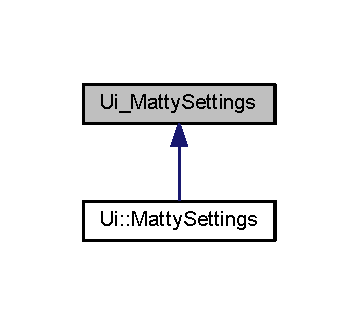
\includegraphics[width=172pt]{classUi__MattySettings__inherit__graph}
\end{center}
\end{figure}
\subsection*{Public Member Functions}
\begin{DoxyCompactItemize}
\item 
void \hyperlink{classUi__MattySettings_aa5a49194b05cc0f4d7f06d99f18e253e}{setup\+Ui} (Q\+Widget $\ast$\hyperlink{classMattySettings}{Matty\+Settings})
\item 
void \hyperlink{classUi__MattySettings_aab5e7bc10516f3837b1c4e5cd33b9a76}{retranslate\+Ui} (Q\+Widget $\ast$\hyperlink{classMattySettings}{Matty\+Settings})
\end{DoxyCompactItemize}
\subsection*{Public Attributes}
\begin{DoxyCompactItemize}
\item 
Q\+Grid\+Layout $\ast$ \hyperlink{classUi__MattySettings_a289ca61cb5fd260abf4fbe3d872f6676}{grid\+Layout}
\end{DoxyCompactItemize}


\subsection{Detailed Description}


Definition at line 22 of file ui\+\_\+mattysettings.\+h.



\subsection{Member Function Documentation}
\hypertarget{classUi__MattySettings_aab5e7bc10516f3837b1c4e5cd33b9a76}{}\label{classUi__MattySettings_aab5e7bc10516f3837b1c4e5cd33b9a76} 
\index{Ui\+\_\+\+Matty\+Settings@{Ui\+\_\+\+Matty\+Settings}!retranslate\+Ui@{retranslate\+Ui}}
\index{retranslate\+Ui@{retranslate\+Ui}!Ui\+\_\+\+Matty\+Settings@{Ui\+\_\+\+Matty\+Settings}}
\subsubsection{\texorpdfstring{retranslate\+Ui()}{retranslateUi()}}
{\footnotesize\ttfamily void Ui\+\_\+\+Matty\+Settings\+::retranslate\+Ui (\begin{DoxyParamCaption}\item[{Q\+Widget $\ast$}]{Matty\+Settings }\end{DoxyParamCaption})\hspace{0.3cm}{\ttfamily [inline]}}



Definition at line 40 of file ui\+\_\+mattysettings.\+h.

Here is the caller graph for this function\+:
\nopagebreak
\begin{figure}[H]
\begin{center}
\leavevmode
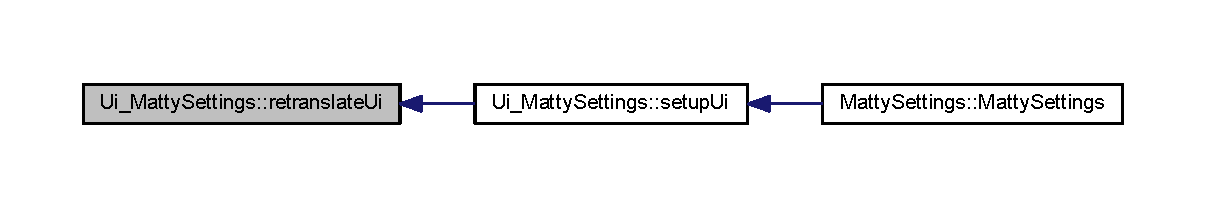
\includegraphics[width=350pt]{classUi__MattySettings_aab5e7bc10516f3837b1c4e5cd33b9a76_icgraph}
\end{center}
\end{figure}
\hypertarget{classUi__MattySettings_aa5a49194b05cc0f4d7f06d99f18e253e}{}\label{classUi__MattySettings_aa5a49194b05cc0f4d7f06d99f18e253e} 
\index{Ui\+\_\+\+Matty\+Settings@{Ui\+\_\+\+Matty\+Settings}!setup\+Ui@{setup\+Ui}}
\index{setup\+Ui@{setup\+Ui}!Ui\+\_\+\+Matty\+Settings@{Ui\+\_\+\+Matty\+Settings}}
\subsubsection{\texorpdfstring{setup\+Ui()}{setupUi()}}
{\footnotesize\ttfamily void Ui\+\_\+\+Matty\+Settings\+::setup\+Ui (\begin{DoxyParamCaption}\item[{Q\+Widget $\ast$}]{Matty\+Settings }\end{DoxyParamCaption})\hspace{0.3cm}{\ttfamily [inline]}}



Definition at line 27 of file ui\+\_\+mattysettings.\+h.

Here is the call graph for this function\+:
\nopagebreak
\begin{figure}[H]
\begin{center}
\leavevmode
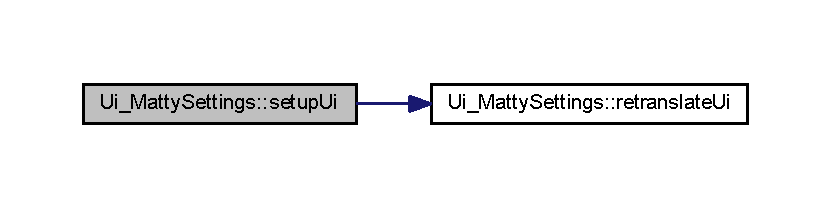
\includegraphics[width=350pt]{classUi__MattySettings_aa5a49194b05cc0f4d7f06d99f18e253e_cgraph}
\end{center}
\end{figure}
Here is the caller graph for this function\+:
\nopagebreak
\begin{figure}[H]
\begin{center}
\leavevmode
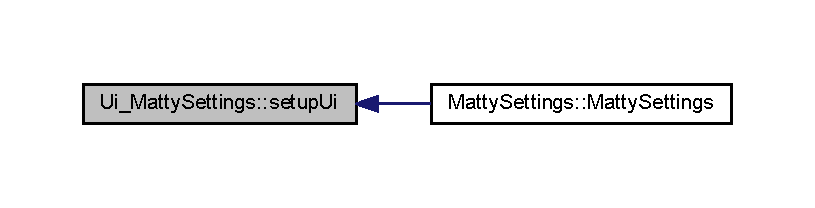
\includegraphics[width=350pt]{classUi__MattySettings_aa5a49194b05cc0f4d7f06d99f18e253e_icgraph}
\end{center}
\end{figure}


\subsection{Member Data Documentation}
\hypertarget{classUi__MattySettings_a289ca61cb5fd260abf4fbe3d872f6676}{}\label{classUi__MattySettings_a289ca61cb5fd260abf4fbe3d872f6676} 
\index{Ui\+\_\+\+Matty\+Settings@{Ui\+\_\+\+Matty\+Settings}!grid\+Layout@{grid\+Layout}}
\index{grid\+Layout@{grid\+Layout}!Ui\+\_\+\+Matty\+Settings@{Ui\+\_\+\+Matty\+Settings}}
\subsubsection{\texorpdfstring{grid\+Layout}{gridLayout}}
{\footnotesize\ttfamily Q\+Grid\+Layout$\ast$ Ui\+\_\+\+Matty\+Settings\+::grid\+Layout}



Definition at line 25 of file ui\+\_\+mattysettings.\+h.



The documentation for this class was generated from the following file\+:\begin{DoxyCompactItemize}
\item 
C\+:/\+Users/\+Ogrigorieva/\+Visual Studio 2015/\+Projects/\+Personal/\+Matty\+Notes/\+Generated\+Files/\hyperlink{ui__mattysettings_8h}{ui\+\_\+mattysettings.\+h}\end{DoxyCompactItemize}

\hypertarget{classUtilityFunctions}{}\section{Utility\+Functions Class Reference}
\label{classUtilityFunctions}\index{Utility\+Functions@{Utility\+Functions}}


{\ttfamily \#include $<$Utility\+Functions.\+h$>$}

\subsection*{Public Member Functions}
\begin{DoxyCompactItemize}
\item 
\hyperlink{classUtilityFunctions_aa66aa28b5c3ee83f8cf14ec56f841443}{Utility\+Functions} ()
\item 
\hyperlink{classUtilityFunctions_ab92ca1da946cc58713f6d06a4bcd0ff6}{$\sim$\+Utility\+Functions} ()
\end{DoxyCompactItemize}
\subsection*{Static Public Member Functions}
\begin{DoxyCompactItemize}
\item 
static Q\+String \hyperlink{classUtilityFunctions_a9decf9e823f96af31a5dac497f2c68d2}{make\+Single\+Double} (int income\+Int)
\item 
static Q\+String \hyperlink{classUtilityFunctions_ac2212f463b34781025e9e0bcfeaad3eb}{repare\+Time} (Q\+String Time\+To\+Repair)
\item 
static Q\+String \hyperlink{classUtilityFunctions_a11f16049e57928c6a74aba7438f66841}{repare\+Date} (Q\+String Date)
\end{DoxyCompactItemize}


\subsection{Detailed Description}


Definition at line 8 of file Utility\+Functions.\+h.



\subsection{Constructor \& Destructor Documentation}
\hypertarget{classUtilityFunctions_aa66aa28b5c3ee83f8cf14ec56f841443}{}\label{classUtilityFunctions_aa66aa28b5c3ee83f8cf14ec56f841443} 
\index{Utility\+Functions@{Utility\+Functions}!Utility\+Functions@{Utility\+Functions}}
\index{Utility\+Functions@{Utility\+Functions}!Utility\+Functions@{Utility\+Functions}}
\subsubsection{\texorpdfstring{Utility\+Functions()}{UtilityFunctions()}}
{\footnotesize\ttfamily Utility\+Functions\+::\+Utility\+Functions (\begin{DoxyParamCaption}{ }\end{DoxyParamCaption})}



Definition at line 5 of file Utility\+Functions.\+cpp.

\hypertarget{classUtilityFunctions_ab92ca1da946cc58713f6d06a4bcd0ff6}{}\label{classUtilityFunctions_ab92ca1da946cc58713f6d06a4bcd0ff6} 
\index{Utility\+Functions@{Utility\+Functions}!````~Utility\+Functions@{$\sim$\+Utility\+Functions}}
\index{````~Utility\+Functions@{$\sim$\+Utility\+Functions}!Utility\+Functions@{Utility\+Functions}}
\subsubsection{\texorpdfstring{$\sim$\+Utility\+Functions()}{~UtilityFunctions()}}
{\footnotesize\ttfamily Utility\+Functions\+::$\sim$\+Utility\+Functions (\begin{DoxyParamCaption}{ }\end{DoxyParamCaption})}



Definition at line 54 of file Utility\+Functions.\+cpp.



\subsection{Member Function Documentation}
\hypertarget{classUtilityFunctions_a9decf9e823f96af31a5dac497f2c68d2}{}\label{classUtilityFunctions_a9decf9e823f96af31a5dac497f2c68d2} 
\index{Utility\+Functions@{Utility\+Functions}!make\+Single\+Double@{make\+Single\+Double}}
\index{make\+Single\+Double@{make\+Single\+Double}!Utility\+Functions@{Utility\+Functions}}
\subsubsection{\texorpdfstring{make\+Single\+Double()}{makeSingleDouble()}}
{\footnotesize\ttfamily Q\+String Utility\+Functions\+::make\+Single\+Double (\begin{DoxyParamCaption}\item[{int}]{income\+Int }\end{DoxyParamCaption})\hspace{0.3cm}{\ttfamily [static]}}



Definition at line 9 of file Utility\+Functions.\+cpp.

Here is the caller graph for this function\+:
% FIG 0
\hypertarget{classUtilityFunctions_a11f16049e57928c6a74aba7438f66841}{}\label{classUtilityFunctions_a11f16049e57928c6a74aba7438f66841} 
\index{Utility\+Functions@{Utility\+Functions}!repare\+Date@{repare\+Date}}
\index{repare\+Date@{repare\+Date}!Utility\+Functions@{Utility\+Functions}}
\subsubsection{\texorpdfstring{repare\+Date()}{repareDate()}}
{\footnotesize\ttfamily Q\+String Utility\+Functions\+::repare\+Date (\begin{DoxyParamCaption}\item[{Q\+String}]{Date }\end{DoxyParamCaption})\hspace{0.3cm}{\ttfamily [static]}}



Definition at line 49 of file Utility\+Functions.\+cpp.

\hypertarget{classUtilityFunctions_ac2212f463b34781025e9e0bcfeaad3eb}{}\label{classUtilityFunctions_ac2212f463b34781025e9e0bcfeaad3eb} 
\index{Utility\+Functions@{Utility\+Functions}!repare\+Time@{repare\+Time}}
\index{repare\+Time@{repare\+Time}!Utility\+Functions@{Utility\+Functions}}
\subsubsection{\texorpdfstring{repare\+Time()}{repareTime()}}
{\footnotesize\ttfamily Q\+String Utility\+Functions\+::repare\+Time (\begin{DoxyParamCaption}\item[{Q\+String}]{Time\+To\+Repair }\end{DoxyParamCaption})\hspace{0.3cm}{\ttfamily [static]}}



Definition at line 17 of file Utility\+Functions.\+cpp.

Here is the caller graph for this function\+:
% FIG 1


The documentation for this class was generated from the following files\+:\begin{DoxyCompactItemize}
\item 
C\+:/\+Users/\+Ogrigorieva/\+Visual Studio 2015/\+Projects/\+Personal/\+Matty\+Notes/\hyperlink{UtilityFunctions_8h}{Utility\+Functions.\+h}\item 
C\+:/\+Users/\+Ogrigorieva/\+Visual Studio 2015/\+Projects/\+Personal/\+Matty\+Notes/\hyperlink{UtilityFunctions_8cpp}{Utility\+Functions.\+cpp}\end{DoxyCompactItemize}

\chapter{File Documentation}
\hypertarget{addnotedialog_8cpp}{}\section{C\+:/\+Users/\+Ogrigorieva/\+Visual Studio 2015/\+Projects/\+Personal/\+Matty\+Notes/addnotedialog.cpp File Reference}
\label{addnotedialog_8cpp}\index{C\+:/\+Users/\+Ogrigorieva/\+Visual Studio 2015/\+Projects/\+Personal/\+Matty\+Notes/addnotedialog.\+cpp@{C\+:/\+Users/\+Ogrigorieva/\+Visual Studio 2015/\+Projects/\+Personal/\+Matty\+Notes/addnotedialog.\+cpp}}
{\ttfamily \#include $<$stdafx.\+h$>$}\newline
{\ttfamily \#include \char`\"{}addnotedialog.\+h\char`\"{}}\newline
{\ttfamily \#include \char`\"{}Db\+Manager.\+h\char`\"{}}\newline
{\ttfamily \#include \char`\"{}Matty\+Note.\+h\char`\"{}}\newline
{\ttfamily \#include \char`\"{}Utility\+Functions.\+h\char`\"{}}\newline
{\ttfamily \#include \char`\"{}mattynotes.\+h\char`\"{}}\newline
{\ttfamily \#include \char`\"{}Note\+Holder.\+h\char`\"{}}\newline
{\ttfamily \#include \char`\"{}Constants.\+h\char`\"{}}\newline
Include dependency graph for addnotedialog.\+cpp\+:
\nopagebreak
\begin{figure}[H]
\begin{center}
\leavevmode
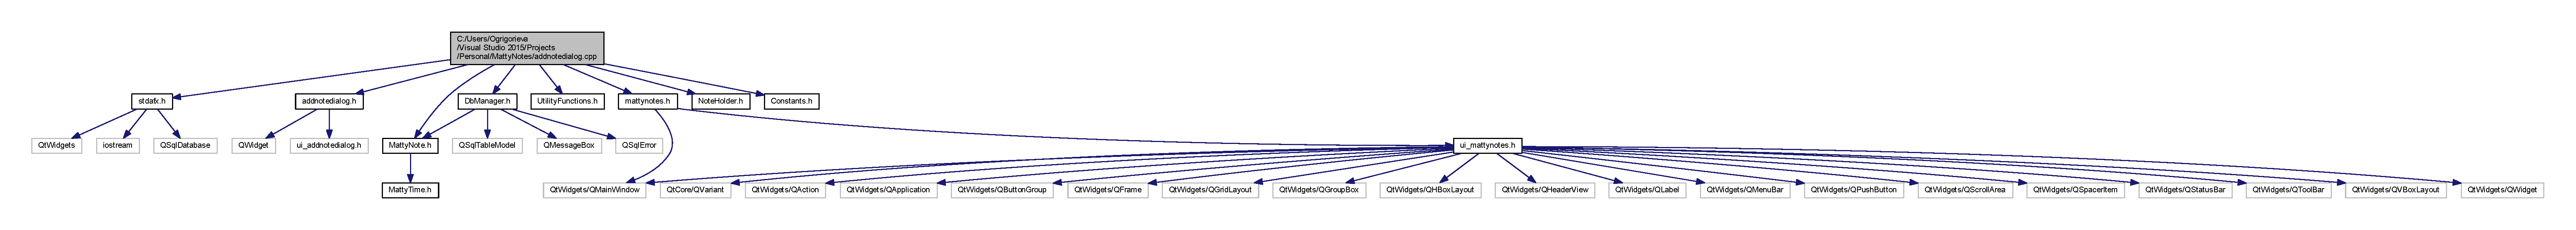
\includegraphics[width=350pt]{addnotedialog_8cpp__incl}
\end{center}
\end{figure}

\hypertarget{addnotedialog_8h}{}\section{C\+:/\+Users/\+Ogrigorieva/\+Visual Studio 2015/\+Projects/\+Personal/\+Matty\+Notes/addnotedialog.h File Reference}
\label{addnotedialog_8h}\index{C\+:/\+Users/\+Ogrigorieva/\+Visual Studio 2015/\+Projects/\+Personal/\+Matty\+Notes/addnotedialog.\+h@{C\+:/\+Users/\+Ogrigorieva/\+Visual Studio 2015/\+Projects/\+Personal/\+Matty\+Notes/addnotedialog.\+h}}
{\ttfamily \#include $<$Q\+Widget$>$}\newline
{\ttfamily \#include \char`\"{}ui\+\_\+addnotedialog.\+h\char`\"{}}\newline
Include dependency graph for addnotedialog.\+h\+:
\nopagebreak
\begin{figure}[H]
\begin{center}
\leavevmode
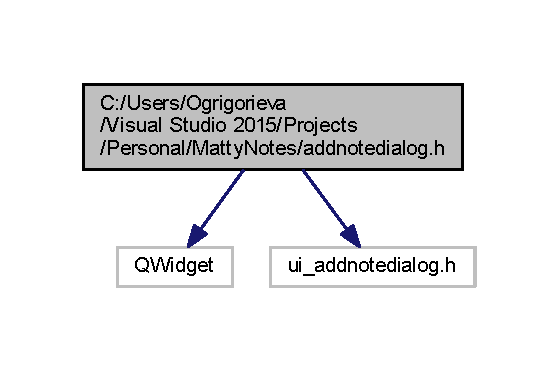
\includegraphics[width=268pt]{addnotedialog_8h__incl}
\end{center}
\end{figure}
This graph shows which files directly or indirectly include this file\+:
\nopagebreak
\begin{figure}[H]
\begin{center}
\leavevmode
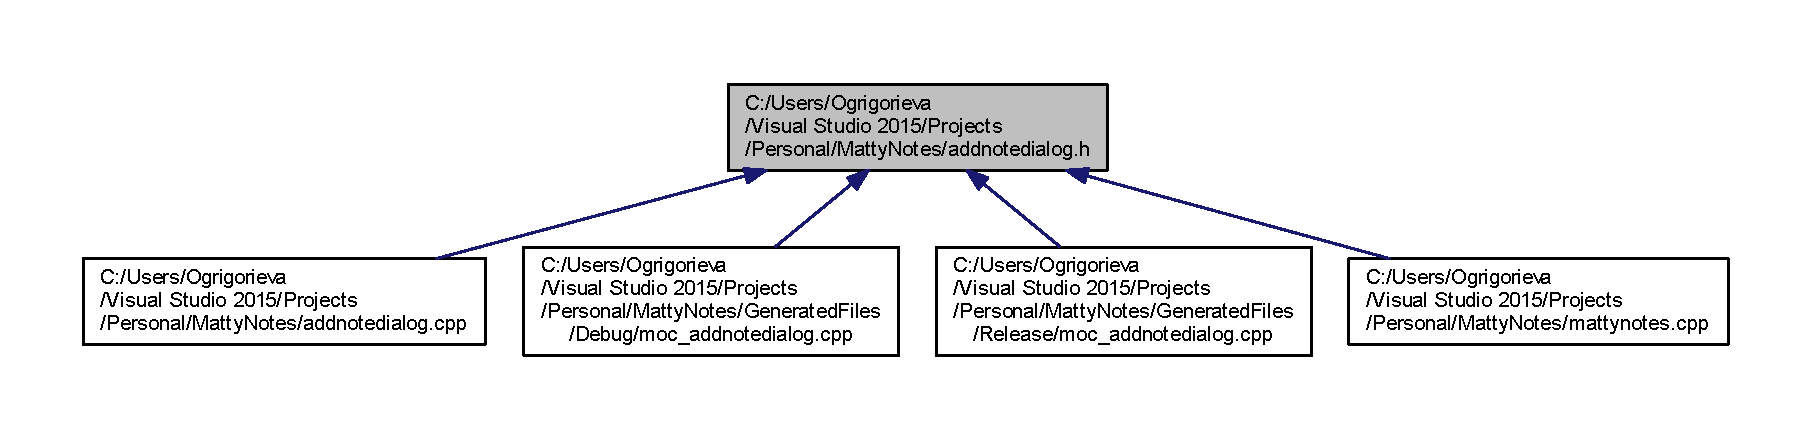
\includegraphics[width=350pt]{addnotedialog_8h__dep__incl}
\end{center}
\end{figure}
\subsection*{Classes}
\begin{DoxyCompactItemize}
\item 
class \hyperlink{classaddNoteDialog}{add\+Note\+Dialog}
\end{DoxyCompactItemize}

\hypertarget{Constants_8cpp}{}\section{C\+:/\+Users/\+Ogrigorieva/\+Visual Studio 2015/\+Projects/\+Personal/\+Matty\+Notes/\+Constants.cpp File Reference}
\label{Constants_8cpp}\index{C\+:/\+Users/\+Ogrigorieva/\+Visual Studio 2015/\+Projects/\+Personal/\+Matty\+Notes/\+Constants.\+cpp@{C\+:/\+Users/\+Ogrigorieva/\+Visual Studio 2015/\+Projects/\+Personal/\+Matty\+Notes/\+Constants.\+cpp}}
{\ttfamily \#include \char`\"{}stdafx.\+h\char`\"{}}\newline
{\ttfamily \#include \char`\"{}Constants.\+h\char`\"{}}\newline
Include dependency graph for Constants.\+cpp\+:
% FIG 0

\hypertarget{Constants_8h}{}\section{C\+:/\+Users/\+Ogrigorieva/\+Visual Studio 2015/\+Projects/\+Personal/\+Matty\+Notes/\+Constants.h File Reference}
\label{Constants_8h}\index{C\+:/\+Users/\+Ogrigorieva/\+Visual Studio 2015/\+Projects/\+Personal/\+Matty\+Notes/\+Constants.\+h@{C\+:/\+Users/\+Ogrigorieva/\+Visual Studio 2015/\+Projects/\+Personal/\+Matty\+Notes/\+Constants.\+h}}
This graph shows which files directly or indirectly include this file\+:
% FIG 0
\subsection*{Classes}
\begin{DoxyCompactItemize}
\item 
class \hyperlink{classConstants}{Constants}
\end{DoxyCompactItemize}
\subsection*{Enumerations}
\begin{DoxyCompactItemize}
\item 
enum \hyperlink{Constants_8h_a9558e0854b1cdaf803f7a80df80ab91b}{Matty\+Path\+To\+Db\+Type} \{ \hyperlink{Constants_8h_a9558e0854b1cdaf803f7a80df80ab91ba9896adb26d900426b91a564bdac5deed}{Home\+Absolute}, 
\hyperlink{Constants_8h_a9558e0854b1cdaf803f7a80df80ab91baef13eb429730a3a3bea647eb7324d6f3}{Work\+Absolute}, 
\hyperlink{Constants_8h_a9558e0854b1cdaf803f7a80df80ab91ba0f23d10f26a8446d64fded7b7478bee7}{Relative}
 \}
\end{DoxyCompactItemize}


\subsection{Enumeration Type Documentation}
\hypertarget{Constants_8h_a9558e0854b1cdaf803f7a80df80ab91b}{}\label{Constants_8h_a9558e0854b1cdaf803f7a80df80ab91b} 
\index{Constants.\+h@{Constants.\+h}!Matty\+Path\+To\+Db\+Type@{Matty\+Path\+To\+Db\+Type}}
\index{Matty\+Path\+To\+Db\+Type@{Matty\+Path\+To\+Db\+Type}!Constants.\+h@{Constants.\+h}}
\subsubsection{\texorpdfstring{Matty\+Path\+To\+Db\+Type}{MattyPathToDbType}}
{\footnotesize\ttfamily enum \hyperlink{Constants_8h_a9558e0854b1cdaf803f7a80df80ab91b}{Matty\+Path\+To\+Db\+Type}}

\begin{DoxyEnumFields}{Enumerator}
\raisebox{\heightof{T}}[0pt][0pt]{\index{Home\+Absolute@{Home\+Absolute}!Constants.\+h@{Constants.\+h}}\index{Constants.\+h@{Constants.\+h}!Home\+Absolute@{Home\+Absolute}}}\hypertarget{Constants_8h_a9558e0854b1cdaf803f7a80df80ab91ba9896adb26d900426b91a564bdac5deed}{}\label{Constants_8h_a9558e0854b1cdaf803f7a80df80ab91ba9896adb26d900426b91a564bdac5deed} 
Home\+Absolute&\\
\hline

\raisebox{\heightof{T}}[0pt][0pt]{\index{Work\+Absolute@{Work\+Absolute}!Constants.\+h@{Constants.\+h}}\index{Constants.\+h@{Constants.\+h}!Work\+Absolute@{Work\+Absolute}}}\hypertarget{Constants_8h_a9558e0854b1cdaf803f7a80df80ab91baef13eb429730a3a3bea647eb7324d6f3}{}\label{Constants_8h_a9558e0854b1cdaf803f7a80df80ab91baef13eb429730a3a3bea647eb7324d6f3} 
Work\+Absolute&\\
\hline

\raisebox{\heightof{T}}[0pt][0pt]{\index{Relative@{Relative}!Constants.\+h@{Constants.\+h}}\index{Constants.\+h@{Constants.\+h}!Relative@{Relative}}}\hypertarget{Constants_8h_a9558e0854b1cdaf803f7a80df80ab91ba0f23d10f26a8446d64fded7b7478bee7}{}\label{Constants_8h_a9558e0854b1cdaf803f7a80df80ab91ba0f23d10f26a8446d64fded7b7478bee7} 
Relative&\\
\hline

\end{DoxyEnumFields}


Definition at line 8 of file Constants.\+h.


\hypertarget{DbManager_8cpp}{}\section{C\+:/\+Users/\+Ogrigorieva/\+Visual Studio 2015/\+Projects/\+Personal/\+Matty\+Notes/\+Db\+Manager.cpp File Reference}
\label{DbManager_8cpp}\index{C\+:/\+Users/\+Ogrigorieva/\+Visual Studio 2015/\+Projects/\+Personal/\+Matty\+Notes/\+Db\+Manager.\+cpp@{C\+:/\+Users/\+Ogrigorieva/\+Visual Studio 2015/\+Projects/\+Personal/\+Matty\+Notes/\+Db\+Manager.\+cpp}}
{\ttfamily \#include \char`\"{}stdafx.\+h\char`\"{}}\newline
{\ttfamily \#include \char`\"{}Db\+Manager.\+h\char`\"{}}\newline
{\ttfamily \#include $<$Q\+Sql\+Query$>$}\newline
{\ttfamily \#include $<$Q\+Sql\+Record$>$}\newline
Include dependency graph for Db\+Manager.\+cpp\+:
\nopagebreak
\begin{figure}[H]
\begin{center}
\leavevmode
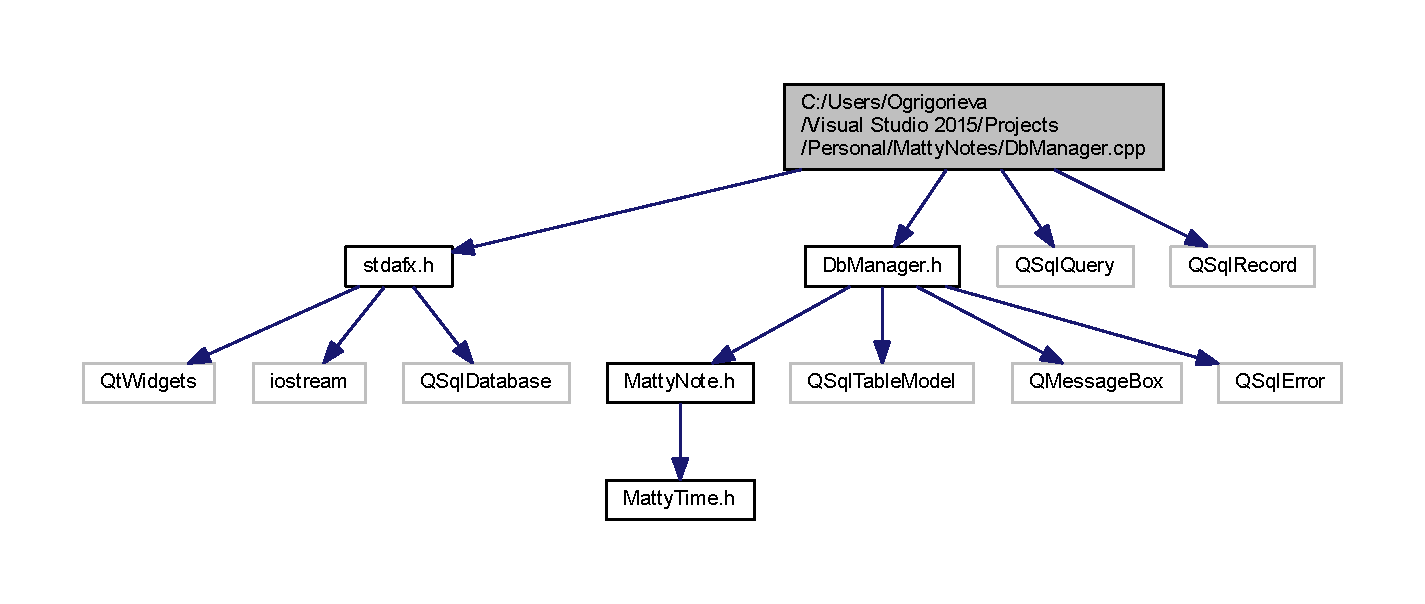
\includegraphics[width=350pt]{DbManager_8cpp__incl}
\end{center}
\end{figure}

\hypertarget{DbManager_8h}{}\section{C\+:/\+Users/\+Ogrigorieva/\+Visual Studio 2015/\+Projects/\+Personal/\+Matty\+Notes/\+Db\+Manager.h File Reference}
\label{DbManager_8h}\index{C\+:/\+Users/\+Ogrigorieva/\+Visual Studio 2015/\+Projects/\+Personal/\+Matty\+Notes/\+Db\+Manager.\+h@{C\+:/\+Users/\+Ogrigorieva/\+Visual Studio 2015/\+Projects/\+Personal/\+Matty\+Notes/\+Db\+Manager.\+h}}
{\ttfamily \#include \char`\"{}Matty\+Note.\+h\char`\"{}}\newline
{\ttfamily \#include $<$Q\+Sql\+Table\+Model$>$}\newline
{\ttfamily \#include $<$Q\+Message\+Box$>$}\newline
{\ttfamily \#include $<$Q\+Sql\+Error$>$}\newline
Include dependency graph for Db\+Manager.\+h\+:
% FIG 0
This graph shows which files directly or indirectly include this file\+:
% FIG 1
\subsection*{Classes}
\begin{DoxyCompactItemize}
\item 
class \hyperlink{classDbManager}{Db\+Manager}
\end{DoxyCompactItemize}

\hypertarget{Debug_2moc__addnotedialog_8cpp}{}\section{C\+:/\+Users/\+Ogrigorieva/\+Visual Studio 2015/\+Projects/\+Personal/\+Matty\+Notes/\+Generated\+Files/\+Debug/moc\+\_\+addnotedialog.cpp File Reference}
\label{Debug_2moc__addnotedialog_8cpp}\index{C\+:/\+Users/\+Ogrigorieva/\+Visual Studio 2015/\+Projects/\+Personal/\+Matty\+Notes/\+Generated\+Files/\+Debug/moc\+\_\+addnotedialog.\+cpp@{C\+:/\+Users/\+Ogrigorieva/\+Visual Studio 2015/\+Projects/\+Personal/\+Matty\+Notes/\+Generated\+Files/\+Debug/moc\+\_\+addnotedialog.\+cpp}}
{\ttfamily \#include \char`\"{}stdafx.\+h\char`\"{}}\newline
{\ttfamily \#include \char`\"{}../../addnotedialog.\+h\char`\"{}}\newline
{\ttfamily \#include $<$Qt\+Core/qbytearray.\+h$>$}\newline
{\ttfamily \#include $<$Qt\+Core/qmetatype.\+h$>$}\newline
Include dependency graph for moc\+\_\+addnotedialog.\+cpp\+:
\nopagebreak
\begin{figure}[H]
\begin{center}
\leavevmode
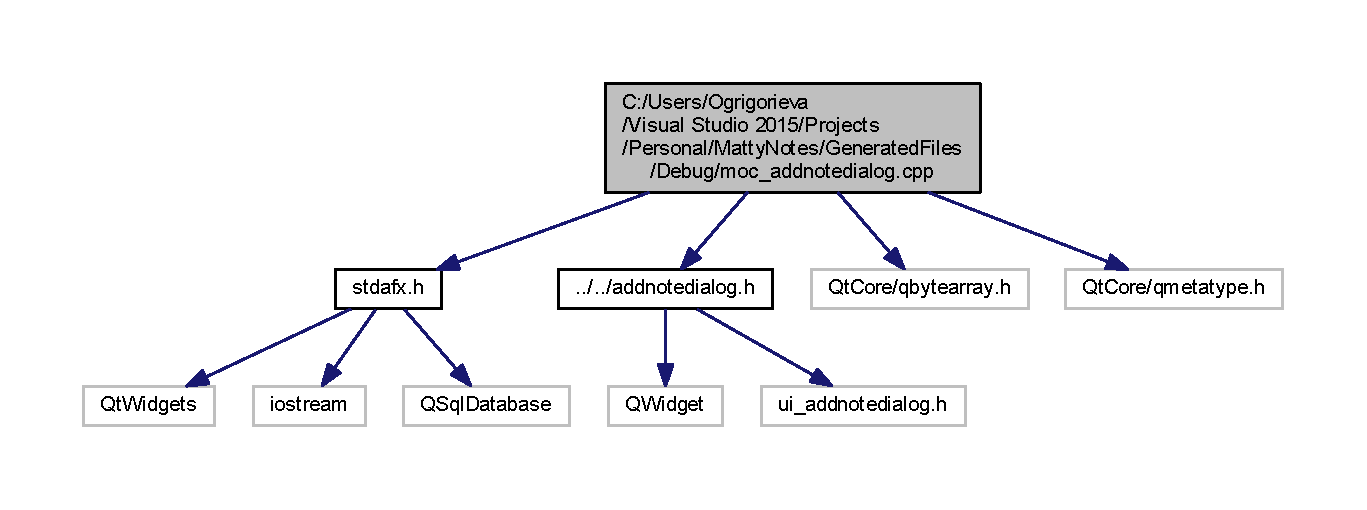
\includegraphics[width=350pt]{Debug_2moc__addnotedialog_8cpp__incl}
\end{center}
\end{figure}
\subsection*{Classes}
\begin{DoxyCompactItemize}
\item 
struct \hyperlink{structqt__meta__stringdata__addNoteDialog__t}{qt\+\_\+meta\+\_\+stringdata\+\_\+add\+Note\+Dialog\+\_\+t}
\end{DoxyCompactItemize}
\subsection*{Macros}
\begin{DoxyCompactItemize}
\item 
\#define \hyperlink{Debug_2moc__addnotedialog_8cpp_a75bb9482d242cde0a06c9dbdc6b83abe}{Q\+T\+\_\+\+M\+O\+C\+\_\+\+L\+I\+T\+E\+R\+AL}(idx,  ofs,  len)
\end{DoxyCompactItemize}
\subsection*{Variables}
\begin{DoxyCompactItemize}
\item 
static const \hyperlink{structqt__meta__stringdata__addNoteDialog__t}{qt\+\_\+meta\+\_\+stringdata\+\_\+add\+Note\+Dialog\+\_\+t} \hyperlink{Debug_2moc__addnotedialog_8cpp_a0fede77edae452849d17ceb7c0760841}{qt\+\_\+meta\+\_\+stringdata\+\_\+add\+Note\+Dialog}
\item 
static const uint \hyperlink{Debug_2moc__addnotedialog_8cpp_a30733ac3aa6f774f42c680fffa0df084}{qt\+\_\+meta\+\_\+data\+\_\+add\+Note\+Dialog} \mbox{[}$\,$\mbox{]}
\end{DoxyCompactItemize}


\subsection{Macro Definition Documentation}
\hypertarget{Debug_2moc__addnotedialog_8cpp_a75bb9482d242cde0a06c9dbdc6b83abe}{}\label{Debug_2moc__addnotedialog_8cpp_a75bb9482d242cde0a06c9dbdc6b83abe} 
\index{Debug/moc\+\_\+addnotedialog.\+cpp@{Debug/moc\+\_\+addnotedialog.\+cpp}!Q\+T\+\_\+\+M\+O\+C\+\_\+\+L\+I\+T\+E\+R\+AL@{Q\+T\+\_\+\+M\+O\+C\+\_\+\+L\+I\+T\+E\+R\+AL}}
\index{Q\+T\+\_\+\+M\+O\+C\+\_\+\+L\+I\+T\+E\+R\+AL@{Q\+T\+\_\+\+M\+O\+C\+\_\+\+L\+I\+T\+E\+R\+AL}!Debug/moc\+\_\+addnotedialog.\+cpp@{Debug/moc\+\_\+addnotedialog.\+cpp}}
\subsubsection{\texorpdfstring{Q\+T\+\_\+\+M\+O\+C\+\_\+\+L\+I\+T\+E\+R\+AL}{QT\_MOC\_LITERAL}}
{\footnotesize\ttfamily \#define Q\+T\+\_\+\+M\+O\+C\+\_\+\+L\+I\+T\+E\+R\+AL(\begin{DoxyParamCaption}\item[{}]{idx,  }\item[{}]{ofs,  }\item[{}]{len }\end{DoxyParamCaption})}

{\bfseries Value\+:}
\begin{DoxyCode}
Q\_STATIC\_BYTE\_ARRAY\_DATA\_HEADER\_INITIALIZER\_WITH\_OFFSET(len, \(\backslash\)
    qptrdiff(offsetof(\hyperlink{structqt__meta__stringdata__addNoteDialog__t}{qt\_meta\_stringdata\_addNoteDialog\_t}, stringdata0) + 
      ofs \(\backslash\)
        - idx * \textcolor{keyword}{sizeof}(QByteArrayData)) \(\backslash\)
    )
\end{DoxyCode}


Definition at line 26 of file moc\+\_\+addnotedialog.\+cpp.



\subsection{Variable Documentation}
\hypertarget{Debug_2moc__addnotedialog_8cpp_a30733ac3aa6f774f42c680fffa0df084}{}\label{Debug_2moc__addnotedialog_8cpp_a30733ac3aa6f774f42c680fffa0df084} 
\index{Debug/moc\+\_\+addnotedialog.\+cpp@{Debug/moc\+\_\+addnotedialog.\+cpp}!qt\+\_\+meta\+\_\+data\+\_\+add\+Note\+Dialog@{qt\+\_\+meta\+\_\+data\+\_\+add\+Note\+Dialog}}
\index{qt\+\_\+meta\+\_\+data\+\_\+add\+Note\+Dialog@{qt\+\_\+meta\+\_\+data\+\_\+add\+Note\+Dialog}!Debug/moc\+\_\+addnotedialog.\+cpp@{Debug/moc\+\_\+addnotedialog.\+cpp}}
\subsubsection{\texorpdfstring{qt\+\_\+meta\+\_\+data\+\_\+add\+Note\+Dialog}{qt\_meta\_data\_addNoteDialog}}
{\footnotesize\ttfamily const uint qt\+\_\+meta\+\_\+data\+\_\+add\+Note\+Dialog\mbox{[}$\,$\mbox{]}\hspace{0.3cm}{\ttfamily [static]}}

{\bfseries Initial value\+:}
\begin{DoxyCode}
= \{

 
       7,       
       0,       
       0,    0, 
       2,   14, 
       0,    0, 
       0,    0, 
       0,    0, 
       0,       
       0,       

 
       1,    0,   24,    2, 0x08 ,
       3,    0,   25,    2, 0x08 ,

 
    QMetaType::Void,
    QMetaType::Void,

       0        
\}
\end{DoxyCode}


Definition at line 44 of file moc\+\_\+addnotedialog.\+cpp.

\hypertarget{Debug_2moc__addnotedialog_8cpp_a0fede77edae452849d17ceb7c0760841}{}\label{Debug_2moc__addnotedialog_8cpp_a0fede77edae452849d17ceb7c0760841} 
\index{Debug/moc\+\_\+addnotedialog.\+cpp@{Debug/moc\+\_\+addnotedialog.\+cpp}!qt\+\_\+meta\+\_\+stringdata\+\_\+add\+Note\+Dialog@{qt\+\_\+meta\+\_\+stringdata\+\_\+add\+Note\+Dialog}}
\index{qt\+\_\+meta\+\_\+stringdata\+\_\+add\+Note\+Dialog@{qt\+\_\+meta\+\_\+stringdata\+\_\+add\+Note\+Dialog}!Debug/moc\+\_\+addnotedialog.\+cpp@{Debug/moc\+\_\+addnotedialog.\+cpp}}
\subsubsection{\texorpdfstring{qt\+\_\+meta\+\_\+stringdata\+\_\+add\+Note\+Dialog}{qt\_meta\_stringdata\_addNoteDialog}}
{\footnotesize\ttfamily const \hyperlink{structqt__meta__stringdata__addNoteDialog__t}{qt\+\_\+meta\+\_\+stringdata\+\_\+add\+Note\+Dialog\+\_\+t} qt\+\_\+meta\+\_\+stringdata\+\_\+add\+Note\+Dialog\hspace{0.3cm}{\ttfamily [static]}}

{\bfseries Initial value\+:}
\begin{DoxyCode}
= \{
    \{
\hyperlink{Debug_2moc__addnotedialog_8cpp_a75bb9482d242cde0a06c9dbdc6b83abe}{QT\_MOC\_LITERAL}(0, 0, 13), 
\hyperlink{Debug_2moc__addnotedialog_8cpp_a75bb9482d242cde0a06c9dbdc6b83abe}{QT\_MOC\_LITERAL}(1, 14, 27), 
\hyperlink{Debug_2moc__addnotedialog_8cpp_a75bb9482d242cde0a06c9dbdc6b83abe}{QT\_MOC\_LITERAL}(2, 42, 0), 
\hyperlink{Debug_2moc__addnotedialog_8cpp_a75bb9482d242cde0a06c9dbdc6b83abe}{QT\_MOC\_LITERAL}(3, 43, 33) 

    \},
    \textcolor{stringliteral}{"addNoteDialog\(\backslash\)0on\_createNoteButton\_clicked\(\backslash\)0"}
    \textcolor{stringliteral}{"\(\backslash\)0on\_cancelAddingNoteButton\_clicked"}
\}
\end{DoxyCode}


Definition at line 31 of file moc\+\_\+addnotedialog.\+cpp.


\hypertarget{Release_2moc__addnotedialog_8cpp}{}\section{C\+:/\+Users/\+Ogrigorieva/\+Visual Studio 2015/\+Projects/\+Personal/\+Matty\+Notes/\+Generated\+Files/\+Release/moc\+\_\+addnotedialog.cpp File Reference}
\label{Release_2moc__addnotedialog_8cpp}\index{C\+:/\+Users/\+Ogrigorieva/\+Visual Studio 2015/\+Projects/\+Personal/\+Matty\+Notes/\+Generated\+Files/\+Release/moc\+\_\+addnotedialog.\+cpp@{C\+:/\+Users/\+Ogrigorieva/\+Visual Studio 2015/\+Projects/\+Personal/\+Matty\+Notes/\+Generated\+Files/\+Release/moc\+\_\+addnotedialog.\+cpp}}
{\ttfamily \#include \char`\"{}stdafx.\+h\char`\"{}}\newline
{\ttfamily \#include \char`\"{}../../addnotedialog.\+h\char`\"{}}\newline
{\ttfamily \#include $<$Qt\+Core/qbytearray.\+h$>$}\newline
{\ttfamily \#include $<$Qt\+Core/qmetatype.\+h$>$}\newline
Include dependency graph for moc\+\_\+addnotedialog.\+cpp\+:
\nopagebreak
\begin{figure}[H]
\begin{center}
\leavevmode
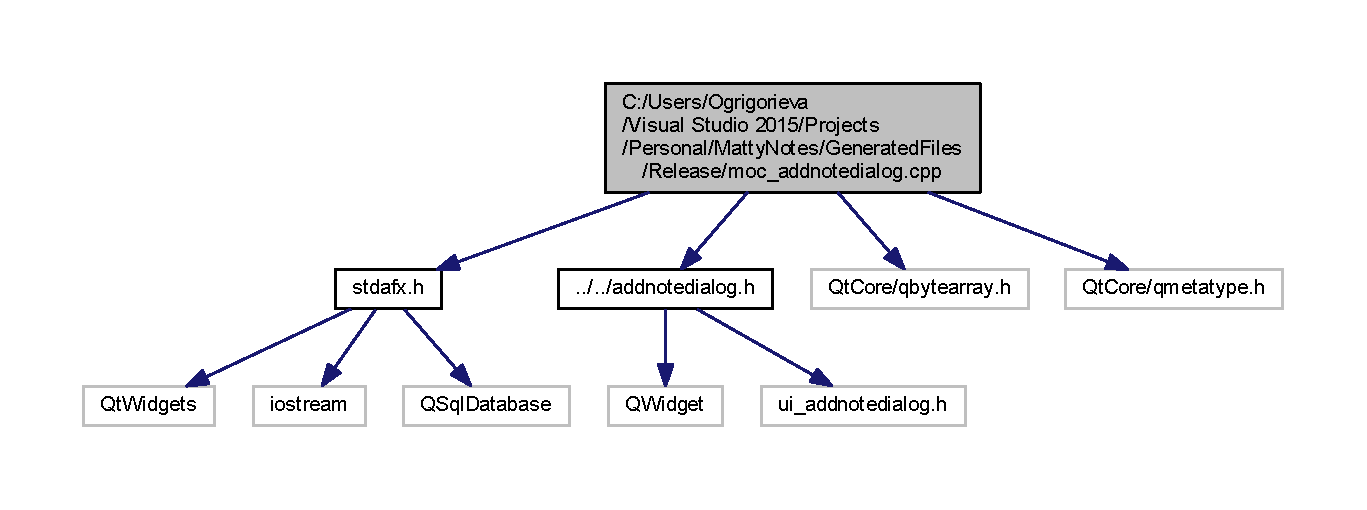
\includegraphics[width=350pt]{Release_2moc__addnotedialog_8cpp__incl}
\end{center}
\end{figure}
\subsection*{Classes}
\begin{DoxyCompactItemize}
\item 
struct \hyperlink{structqt__meta__stringdata__addNoteDialog__t}{qt\+\_\+meta\+\_\+stringdata\+\_\+add\+Note\+Dialog\+\_\+t}
\end{DoxyCompactItemize}
\subsection*{Macros}
\begin{DoxyCompactItemize}
\item 
\#define \hyperlink{Release_2moc__addnotedialog_8cpp_a75bb9482d242cde0a06c9dbdc6b83abe}{Q\+T\+\_\+\+M\+O\+C\+\_\+\+L\+I\+T\+E\+R\+AL}(idx,  ofs,  len)
\end{DoxyCompactItemize}
\subsection*{Variables}
\begin{DoxyCompactItemize}
\item 
static const \hyperlink{structqt__meta__stringdata__addNoteDialog__t}{qt\+\_\+meta\+\_\+stringdata\+\_\+add\+Note\+Dialog\+\_\+t} \hyperlink{Release_2moc__addnotedialog_8cpp_a0fede77edae452849d17ceb7c0760841}{qt\+\_\+meta\+\_\+stringdata\+\_\+add\+Note\+Dialog}
\item 
static const uint \hyperlink{Release_2moc__addnotedialog_8cpp_a30733ac3aa6f774f42c680fffa0df084}{qt\+\_\+meta\+\_\+data\+\_\+add\+Note\+Dialog} \mbox{[}$\,$\mbox{]}
\end{DoxyCompactItemize}


\subsection{Macro Definition Documentation}
\hypertarget{Release_2moc__addnotedialog_8cpp_a75bb9482d242cde0a06c9dbdc6b83abe}{}\label{Release_2moc__addnotedialog_8cpp_a75bb9482d242cde0a06c9dbdc6b83abe} 
\index{Release/moc\+\_\+addnotedialog.\+cpp@{Release/moc\+\_\+addnotedialog.\+cpp}!Q\+T\+\_\+\+M\+O\+C\+\_\+\+L\+I\+T\+E\+R\+AL@{Q\+T\+\_\+\+M\+O\+C\+\_\+\+L\+I\+T\+E\+R\+AL}}
\index{Q\+T\+\_\+\+M\+O\+C\+\_\+\+L\+I\+T\+E\+R\+AL@{Q\+T\+\_\+\+M\+O\+C\+\_\+\+L\+I\+T\+E\+R\+AL}!Release/moc\+\_\+addnotedialog.\+cpp@{Release/moc\+\_\+addnotedialog.\+cpp}}
\subsubsection{\texorpdfstring{Q\+T\+\_\+\+M\+O\+C\+\_\+\+L\+I\+T\+E\+R\+AL}{QT\_MOC\_LITERAL}}
{\footnotesize\ttfamily \#define Q\+T\+\_\+\+M\+O\+C\+\_\+\+L\+I\+T\+E\+R\+AL(\begin{DoxyParamCaption}\item[{}]{idx,  }\item[{}]{ofs,  }\item[{}]{len }\end{DoxyParamCaption})}

{\bfseries Value\+:}
\begin{DoxyCode}
Q\_STATIC\_BYTE\_ARRAY\_DATA\_HEADER\_INITIALIZER\_WITH\_OFFSET(len, \(\backslash\)
    qptrdiff(offsetof(\hyperlink{structqt__meta__stringdata__addNoteDialog__t}{qt\_meta\_stringdata\_addNoteDialog\_t}, stringdata0) + 
      ofs \(\backslash\)
        - idx * \textcolor{keyword}{sizeof}(QByteArrayData)) \(\backslash\)
    )
\end{DoxyCode}


Definition at line 26 of file moc\+\_\+addnotedialog.\+cpp.



\subsection{Variable Documentation}
\hypertarget{Release_2moc__addnotedialog_8cpp_a30733ac3aa6f774f42c680fffa0df084}{}\label{Release_2moc__addnotedialog_8cpp_a30733ac3aa6f774f42c680fffa0df084} 
\index{Release/moc\+\_\+addnotedialog.\+cpp@{Release/moc\+\_\+addnotedialog.\+cpp}!qt\+\_\+meta\+\_\+data\+\_\+add\+Note\+Dialog@{qt\+\_\+meta\+\_\+data\+\_\+add\+Note\+Dialog}}
\index{qt\+\_\+meta\+\_\+data\+\_\+add\+Note\+Dialog@{qt\+\_\+meta\+\_\+data\+\_\+add\+Note\+Dialog}!Release/moc\+\_\+addnotedialog.\+cpp@{Release/moc\+\_\+addnotedialog.\+cpp}}
\subsubsection{\texorpdfstring{qt\+\_\+meta\+\_\+data\+\_\+add\+Note\+Dialog}{qt\_meta\_data\_addNoteDialog}}
{\footnotesize\ttfamily const uint qt\+\_\+meta\+\_\+data\+\_\+add\+Note\+Dialog\mbox{[}$\,$\mbox{]}\hspace{0.3cm}{\ttfamily [static]}}

{\bfseries Initial value\+:}
\begin{DoxyCode}
= \{

 
       7,       
       0,       
       0,    0, 
       2,   14, 
       0,    0, 
       0,    0, 
       0,    0, 
       0,       
       0,       

 
       1,    0,   24,    2, 0x08 ,
       3,    0,   25,    2, 0x08 ,

 
    QMetaType::Void,
    QMetaType::Void,

       0        
\}
\end{DoxyCode}


Definition at line 44 of file moc\+\_\+addnotedialog.\+cpp.

\hypertarget{Release_2moc__addnotedialog_8cpp_a0fede77edae452849d17ceb7c0760841}{}\label{Release_2moc__addnotedialog_8cpp_a0fede77edae452849d17ceb7c0760841} 
\index{Release/moc\+\_\+addnotedialog.\+cpp@{Release/moc\+\_\+addnotedialog.\+cpp}!qt\+\_\+meta\+\_\+stringdata\+\_\+add\+Note\+Dialog@{qt\+\_\+meta\+\_\+stringdata\+\_\+add\+Note\+Dialog}}
\index{qt\+\_\+meta\+\_\+stringdata\+\_\+add\+Note\+Dialog@{qt\+\_\+meta\+\_\+stringdata\+\_\+add\+Note\+Dialog}!Release/moc\+\_\+addnotedialog.\+cpp@{Release/moc\+\_\+addnotedialog.\+cpp}}
\subsubsection{\texorpdfstring{qt\+\_\+meta\+\_\+stringdata\+\_\+add\+Note\+Dialog}{qt\_meta\_stringdata\_addNoteDialog}}
{\footnotesize\ttfamily const \hyperlink{structqt__meta__stringdata__addNoteDialog__t}{qt\+\_\+meta\+\_\+stringdata\+\_\+add\+Note\+Dialog\+\_\+t} qt\+\_\+meta\+\_\+stringdata\+\_\+add\+Note\+Dialog\hspace{0.3cm}{\ttfamily [static]}}

{\bfseries Initial value\+:}
\begin{DoxyCode}
= \{
    \{
\hyperlink{Release_2moc__addnotedialog_8cpp_a75bb9482d242cde0a06c9dbdc6b83abe}{QT\_MOC\_LITERAL}(0, 0, 13), 
\hyperlink{Release_2moc__addnotedialog_8cpp_a75bb9482d242cde0a06c9dbdc6b83abe}{QT\_MOC\_LITERAL}(1, 14, 27), 
\hyperlink{Release_2moc__addnotedialog_8cpp_a75bb9482d242cde0a06c9dbdc6b83abe}{QT\_MOC\_LITERAL}(2, 42, 0), 
\hyperlink{Release_2moc__addnotedialog_8cpp_a75bb9482d242cde0a06c9dbdc6b83abe}{QT\_MOC\_LITERAL}(3, 43, 33) 

    \},
    \textcolor{stringliteral}{"addNoteDialog\(\backslash\)0on\_createNoteButton\_clicked\(\backslash\)0"}
    \textcolor{stringliteral}{"\(\backslash\)0on\_cancelAddingNoteButton\_clicked"}
\}
\end{DoxyCode}


Definition at line 31 of file moc\+\_\+addnotedialog.\+cpp.


\hypertarget{Debug_2moc__MattyGroupBox_8cpp}{}\section{C\+:/\+Users/\+Ogrigorieva/\+Visual Studio 2015/\+Projects/\+Personal/\+Matty\+Notes/\+Generated\+Files/\+Debug/moc\+\_\+\+Matty\+Group\+Box.cpp File Reference}
\label{Debug_2moc__MattyGroupBox_8cpp}\index{C\+:/\+Users/\+Ogrigorieva/\+Visual Studio 2015/\+Projects/\+Personal/\+Matty\+Notes/\+Generated\+Files/\+Debug/moc\+\_\+\+Matty\+Group\+Box.\+cpp@{C\+:/\+Users/\+Ogrigorieva/\+Visual Studio 2015/\+Projects/\+Personal/\+Matty\+Notes/\+Generated\+Files/\+Debug/moc\+\_\+\+Matty\+Group\+Box.\+cpp}}
{\ttfamily \#include \char`\"{}stdafx.\+h\char`\"{}}\newline
{\ttfamily \#include \char`\"{}../../\+Matty\+Group\+Box.\+h\char`\"{}}\newline
{\ttfamily \#include $<$Qt\+Core/qbytearray.\+h$>$}\newline
{\ttfamily \#include $<$Qt\+Core/qmetatype.\+h$>$}\newline
Include dependency graph for moc\+\_\+\+Matty\+Group\+Box.\+cpp\+:
\nopagebreak
\begin{figure}[H]
\begin{center}
\leavevmode
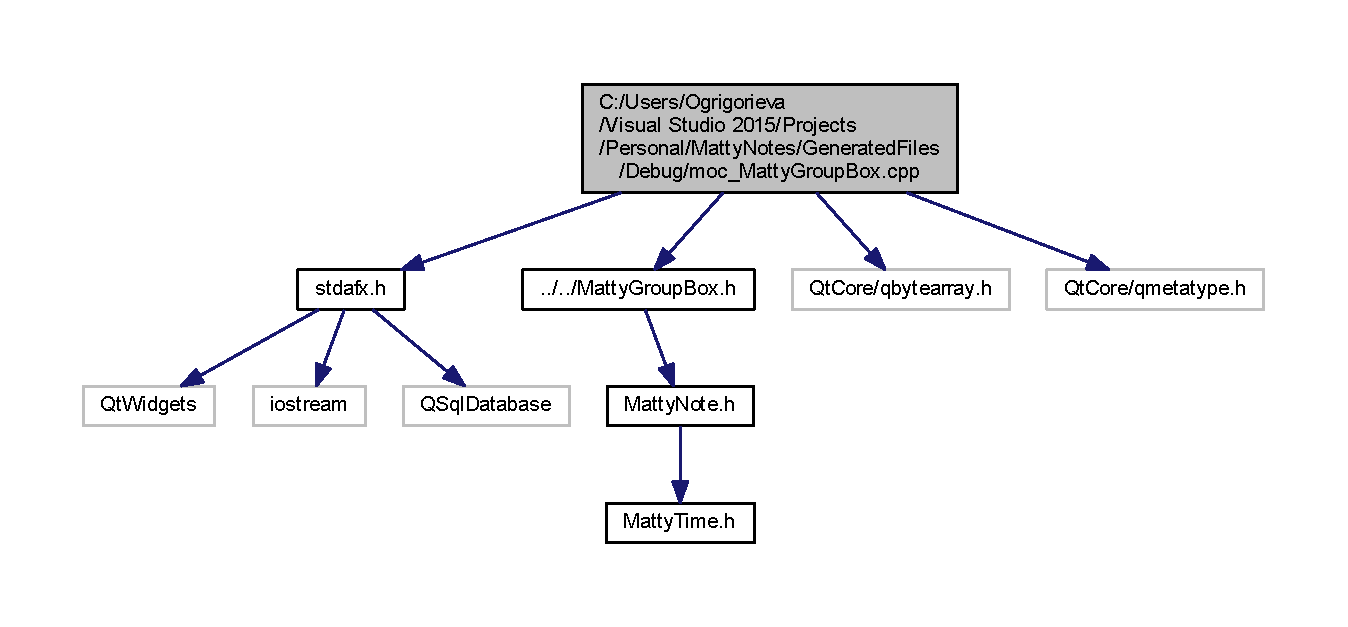
\includegraphics[width=350pt]{Debug_2moc__MattyGroupBox_8cpp__incl}
\end{center}
\end{figure}
\subsection*{Classes}
\begin{DoxyCompactItemize}
\item 
struct \hyperlink{structqt__meta__stringdata__MattyGroupBox__t}{qt\+\_\+meta\+\_\+stringdata\+\_\+\+Matty\+Group\+Box\+\_\+t}
\end{DoxyCompactItemize}
\subsection*{Macros}
\begin{DoxyCompactItemize}
\item 
\#define \hyperlink{Debug_2moc__MattyGroupBox_8cpp_a75bb9482d242cde0a06c9dbdc6b83abe}{Q\+T\+\_\+\+M\+O\+C\+\_\+\+L\+I\+T\+E\+R\+AL}(idx,  ofs,  len)
\end{DoxyCompactItemize}
\subsection*{Variables}
\begin{DoxyCompactItemize}
\item 
static const \hyperlink{structqt__meta__stringdata__MattyGroupBox__t}{qt\+\_\+meta\+\_\+stringdata\+\_\+\+Matty\+Group\+Box\+\_\+t} \hyperlink{Debug_2moc__MattyGroupBox_8cpp_a87846a0ad333e695f5e5d2c5dabdf963}{qt\+\_\+meta\+\_\+stringdata\+\_\+\+Matty\+Group\+Box}
\item 
static const uint \hyperlink{Debug_2moc__MattyGroupBox_8cpp_a21099e22d2d2e12bcab5cca3aac1641f}{qt\+\_\+meta\+\_\+data\+\_\+\+Matty\+Group\+Box} \mbox{[}$\,$\mbox{]}
\end{DoxyCompactItemize}


\subsection{Macro Definition Documentation}
\hypertarget{Debug_2moc__MattyGroupBox_8cpp_a75bb9482d242cde0a06c9dbdc6b83abe}{}\label{Debug_2moc__MattyGroupBox_8cpp_a75bb9482d242cde0a06c9dbdc6b83abe} 
\index{Debug/moc\+\_\+\+Matty\+Group\+Box.\+cpp@{Debug/moc\+\_\+\+Matty\+Group\+Box.\+cpp}!Q\+T\+\_\+\+M\+O\+C\+\_\+\+L\+I\+T\+E\+R\+AL@{Q\+T\+\_\+\+M\+O\+C\+\_\+\+L\+I\+T\+E\+R\+AL}}
\index{Q\+T\+\_\+\+M\+O\+C\+\_\+\+L\+I\+T\+E\+R\+AL@{Q\+T\+\_\+\+M\+O\+C\+\_\+\+L\+I\+T\+E\+R\+AL}!Debug/moc\+\_\+\+Matty\+Group\+Box.\+cpp@{Debug/moc\+\_\+\+Matty\+Group\+Box.\+cpp}}
\subsubsection{\texorpdfstring{Q\+T\+\_\+\+M\+O\+C\+\_\+\+L\+I\+T\+E\+R\+AL}{QT\_MOC\_LITERAL}}
{\footnotesize\ttfamily \#define Q\+T\+\_\+\+M\+O\+C\+\_\+\+L\+I\+T\+E\+R\+AL(\begin{DoxyParamCaption}\item[{}]{idx,  }\item[{}]{ofs,  }\item[{}]{len }\end{DoxyParamCaption})}

{\bfseries Value\+:}
\begin{DoxyCode}
Q\_STATIC\_BYTE\_ARRAY\_DATA\_HEADER\_INITIALIZER\_WITH\_OFFSET(len, \(\backslash\)
    qptrdiff(offsetof(\hyperlink{structqt__meta__stringdata__MattyGroupBox__t}{qt\_meta\_stringdata\_MattyGroupBox\_t}, stringdata0) + 
      ofs \(\backslash\)
        - idx * \textcolor{keyword}{sizeof}(QByteArrayData)) \(\backslash\)
    )
\end{DoxyCode}


Definition at line 26 of file moc\+\_\+\+Matty\+Group\+Box.\+cpp.



\subsection{Variable Documentation}
\hypertarget{Debug_2moc__MattyGroupBox_8cpp_a21099e22d2d2e12bcab5cca3aac1641f}{}\label{Debug_2moc__MattyGroupBox_8cpp_a21099e22d2d2e12bcab5cca3aac1641f} 
\index{Debug/moc\+\_\+\+Matty\+Group\+Box.\+cpp@{Debug/moc\+\_\+\+Matty\+Group\+Box.\+cpp}!qt\+\_\+meta\+\_\+data\+\_\+\+Matty\+Group\+Box@{qt\+\_\+meta\+\_\+data\+\_\+\+Matty\+Group\+Box}}
\index{qt\+\_\+meta\+\_\+data\+\_\+\+Matty\+Group\+Box@{qt\+\_\+meta\+\_\+data\+\_\+\+Matty\+Group\+Box}!Debug/moc\+\_\+\+Matty\+Group\+Box.\+cpp@{Debug/moc\+\_\+\+Matty\+Group\+Box.\+cpp}}
\subsubsection{\texorpdfstring{qt\+\_\+meta\+\_\+data\+\_\+\+Matty\+Group\+Box}{qt\_meta\_data\_MattyGroupBox}}
{\footnotesize\ttfamily const uint qt\+\_\+meta\+\_\+data\+\_\+\+Matty\+Group\+Box\mbox{[}$\,$\mbox{]}\hspace{0.3cm}{\ttfamily [static]}}

{\bfseries Initial value\+:}
\begin{DoxyCode}
= \{

 
       7,       
       0,       
       0,    0, 
       1,   14, 
       0,    0, 
       0,    0, 
       0,    0, 
       0,       
       0,       

 
       1,    0,   19,    2, 0x08 ,

 
    QMetaType::Void,

       0        
\}
\end{DoxyCode}


Definition at line 42 of file moc\+\_\+\+Matty\+Group\+Box.\+cpp.

\hypertarget{Debug_2moc__MattyGroupBox_8cpp_a87846a0ad333e695f5e5d2c5dabdf963}{}\label{Debug_2moc__MattyGroupBox_8cpp_a87846a0ad333e695f5e5d2c5dabdf963} 
\index{Debug/moc\+\_\+\+Matty\+Group\+Box.\+cpp@{Debug/moc\+\_\+\+Matty\+Group\+Box.\+cpp}!qt\+\_\+meta\+\_\+stringdata\+\_\+\+Matty\+Group\+Box@{qt\+\_\+meta\+\_\+stringdata\+\_\+\+Matty\+Group\+Box}}
\index{qt\+\_\+meta\+\_\+stringdata\+\_\+\+Matty\+Group\+Box@{qt\+\_\+meta\+\_\+stringdata\+\_\+\+Matty\+Group\+Box}!Debug/moc\+\_\+\+Matty\+Group\+Box.\+cpp@{Debug/moc\+\_\+\+Matty\+Group\+Box.\+cpp}}
\subsubsection{\texorpdfstring{qt\+\_\+meta\+\_\+stringdata\+\_\+\+Matty\+Group\+Box}{qt\_meta\_stringdata\_MattyGroupBox}}
{\footnotesize\ttfamily const \hyperlink{structqt__meta__stringdata__MattyGroupBox__t}{qt\+\_\+meta\+\_\+stringdata\+\_\+\+Matty\+Group\+Box\+\_\+t} qt\+\_\+meta\+\_\+stringdata\+\_\+\+Matty\+Group\+Box\hspace{0.3cm}{\ttfamily [static]}}

{\bfseries Initial value\+:}
\begin{DoxyCode}
= \{
    \{
\hyperlink{Debug_2moc__MattyGroupBox_8cpp_a75bb9482d242cde0a06c9dbdc6b83abe}{QT\_MOC\_LITERAL}(0, 0, 13), 
\hyperlink{Debug_2moc__MattyGroupBox_8cpp_a75bb9482d242cde0a06c9dbdc6b83abe}{QT\_MOC\_LITERAL}(1, 14, 10), 
\hyperlink{Debug_2moc__MattyGroupBox_8cpp_a75bb9482d242cde0a06c9dbdc6b83abe}{QT\_MOC\_LITERAL}(2, 25, 0) 

    \},
    \textcolor{stringliteral}{"MattyGroupBox\(\backslash\)0deleteNote\(\backslash\)0"}
\}
\end{DoxyCode}


Definition at line 31 of file moc\+\_\+\+Matty\+Group\+Box.\+cpp.


\hypertarget{Release_2moc__MattyGroupBox_8cpp}{}\section{C\+:/\+Users/\+Ogrigorieva/\+Visual Studio 2015/\+Projects/\+Personal/\+Matty\+Notes/\+Generated\+Files/\+Release/moc\+\_\+\+Matty\+Group\+Box.cpp File Reference}
\label{Release_2moc__MattyGroupBox_8cpp}\index{C\+:/\+Users/\+Ogrigorieva/\+Visual Studio 2015/\+Projects/\+Personal/\+Matty\+Notes/\+Generated\+Files/\+Release/moc\+\_\+\+Matty\+Group\+Box.\+cpp@{C\+:/\+Users/\+Ogrigorieva/\+Visual Studio 2015/\+Projects/\+Personal/\+Matty\+Notes/\+Generated\+Files/\+Release/moc\+\_\+\+Matty\+Group\+Box.\+cpp}}
{\ttfamily \#include \char`\"{}stdafx.\+h\char`\"{}}\newline
{\ttfamily \#include \char`\"{}../../\+Matty\+Group\+Box.\+h\char`\"{}}\newline
{\ttfamily \#include $<$Qt\+Core/qbytearray.\+h$>$}\newline
{\ttfamily \#include $<$Qt\+Core/qmetatype.\+h$>$}\newline
Include dependency graph for moc\+\_\+\+Matty\+Group\+Box.\+cpp\+:
\nopagebreak
\begin{figure}[H]
\begin{center}
\leavevmode
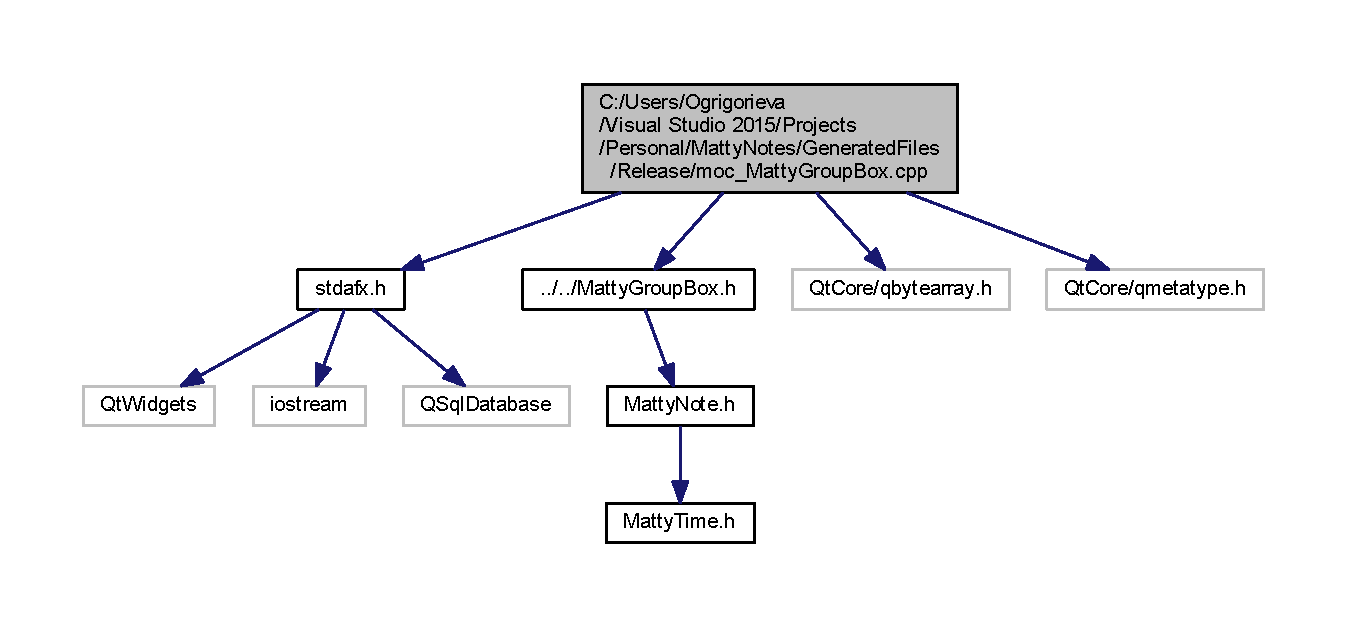
\includegraphics[width=350pt]{Release_2moc__MattyGroupBox_8cpp__incl}
\end{center}
\end{figure}
\subsection*{Classes}
\begin{DoxyCompactItemize}
\item 
struct \hyperlink{structqt__meta__stringdata__MattyGroupBox__t}{qt\+\_\+meta\+\_\+stringdata\+\_\+\+Matty\+Group\+Box\+\_\+t}
\end{DoxyCompactItemize}
\subsection*{Macros}
\begin{DoxyCompactItemize}
\item 
\#define \hyperlink{Release_2moc__MattyGroupBox_8cpp_a75bb9482d242cde0a06c9dbdc6b83abe}{Q\+T\+\_\+\+M\+O\+C\+\_\+\+L\+I\+T\+E\+R\+AL}(idx,  ofs,  len)
\end{DoxyCompactItemize}
\subsection*{Variables}
\begin{DoxyCompactItemize}
\item 
static const \hyperlink{structqt__meta__stringdata__MattyGroupBox__t}{qt\+\_\+meta\+\_\+stringdata\+\_\+\+Matty\+Group\+Box\+\_\+t} \hyperlink{Release_2moc__MattyGroupBox_8cpp_a87846a0ad333e695f5e5d2c5dabdf963}{qt\+\_\+meta\+\_\+stringdata\+\_\+\+Matty\+Group\+Box}
\item 
static const uint \hyperlink{Release_2moc__MattyGroupBox_8cpp_a21099e22d2d2e12bcab5cca3aac1641f}{qt\+\_\+meta\+\_\+data\+\_\+\+Matty\+Group\+Box} \mbox{[}$\,$\mbox{]}
\end{DoxyCompactItemize}


\subsection{Macro Definition Documentation}
\hypertarget{Release_2moc__MattyGroupBox_8cpp_a75bb9482d242cde0a06c9dbdc6b83abe}{}\label{Release_2moc__MattyGroupBox_8cpp_a75bb9482d242cde0a06c9dbdc6b83abe} 
\index{Release/moc\+\_\+\+Matty\+Group\+Box.\+cpp@{Release/moc\+\_\+\+Matty\+Group\+Box.\+cpp}!Q\+T\+\_\+\+M\+O\+C\+\_\+\+L\+I\+T\+E\+R\+AL@{Q\+T\+\_\+\+M\+O\+C\+\_\+\+L\+I\+T\+E\+R\+AL}}
\index{Q\+T\+\_\+\+M\+O\+C\+\_\+\+L\+I\+T\+E\+R\+AL@{Q\+T\+\_\+\+M\+O\+C\+\_\+\+L\+I\+T\+E\+R\+AL}!Release/moc\+\_\+\+Matty\+Group\+Box.\+cpp@{Release/moc\+\_\+\+Matty\+Group\+Box.\+cpp}}
\subsubsection{\texorpdfstring{Q\+T\+\_\+\+M\+O\+C\+\_\+\+L\+I\+T\+E\+R\+AL}{QT\_MOC\_LITERAL}}
{\footnotesize\ttfamily \#define Q\+T\+\_\+\+M\+O\+C\+\_\+\+L\+I\+T\+E\+R\+AL(\begin{DoxyParamCaption}\item[{}]{idx,  }\item[{}]{ofs,  }\item[{}]{len }\end{DoxyParamCaption})}

{\bfseries Value\+:}
\begin{DoxyCode}
Q\_STATIC\_BYTE\_ARRAY\_DATA\_HEADER\_INITIALIZER\_WITH\_OFFSET(len, \(\backslash\)
    qptrdiff(offsetof(\hyperlink{structqt__meta__stringdata__MattyGroupBox__t}{qt\_meta\_stringdata\_MattyGroupBox\_t}, stringdata0) + 
      ofs \(\backslash\)
        - idx * \textcolor{keyword}{sizeof}(QByteArrayData)) \(\backslash\)
    )
\end{DoxyCode}


Definition at line 26 of file moc\+\_\+\+Matty\+Group\+Box.\+cpp.



\subsection{Variable Documentation}
\hypertarget{Release_2moc__MattyGroupBox_8cpp_a21099e22d2d2e12bcab5cca3aac1641f}{}\label{Release_2moc__MattyGroupBox_8cpp_a21099e22d2d2e12bcab5cca3aac1641f} 
\index{Release/moc\+\_\+\+Matty\+Group\+Box.\+cpp@{Release/moc\+\_\+\+Matty\+Group\+Box.\+cpp}!qt\+\_\+meta\+\_\+data\+\_\+\+Matty\+Group\+Box@{qt\+\_\+meta\+\_\+data\+\_\+\+Matty\+Group\+Box}}
\index{qt\+\_\+meta\+\_\+data\+\_\+\+Matty\+Group\+Box@{qt\+\_\+meta\+\_\+data\+\_\+\+Matty\+Group\+Box}!Release/moc\+\_\+\+Matty\+Group\+Box.\+cpp@{Release/moc\+\_\+\+Matty\+Group\+Box.\+cpp}}
\subsubsection{\texorpdfstring{qt\+\_\+meta\+\_\+data\+\_\+\+Matty\+Group\+Box}{qt\_meta\_data\_MattyGroupBox}}
{\footnotesize\ttfamily const uint qt\+\_\+meta\+\_\+data\+\_\+\+Matty\+Group\+Box\mbox{[}$\,$\mbox{]}\hspace{0.3cm}{\ttfamily [static]}}

{\bfseries Initial value\+:}
\begin{DoxyCode}
= \{

 
       7,       
       0,       
       0,    0, 
       1,   14, 
       0,    0, 
       0,    0, 
       0,    0, 
       0,       
       0,       

 
       1,    0,   19,    2, 0x08 ,

 
    QMetaType::Void,

       0        
\}
\end{DoxyCode}


Definition at line 42 of file moc\+\_\+\+Matty\+Group\+Box.\+cpp.

\hypertarget{Release_2moc__MattyGroupBox_8cpp_a87846a0ad333e695f5e5d2c5dabdf963}{}\label{Release_2moc__MattyGroupBox_8cpp_a87846a0ad333e695f5e5d2c5dabdf963} 
\index{Release/moc\+\_\+\+Matty\+Group\+Box.\+cpp@{Release/moc\+\_\+\+Matty\+Group\+Box.\+cpp}!qt\+\_\+meta\+\_\+stringdata\+\_\+\+Matty\+Group\+Box@{qt\+\_\+meta\+\_\+stringdata\+\_\+\+Matty\+Group\+Box}}
\index{qt\+\_\+meta\+\_\+stringdata\+\_\+\+Matty\+Group\+Box@{qt\+\_\+meta\+\_\+stringdata\+\_\+\+Matty\+Group\+Box}!Release/moc\+\_\+\+Matty\+Group\+Box.\+cpp@{Release/moc\+\_\+\+Matty\+Group\+Box.\+cpp}}
\subsubsection{\texorpdfstring{qt\+\_\+meta\+\_\+stringdata\+\_\+\+Matty\+Group\+Box}{qt\_meta\_stringdata\_MattyGroupBox}}
{\footnotesize\ttfamily const \hyperlink{structqt__meta__stringdata__MattyGroupBox__t}{qt\+\_\+meta\+\_\+stringdata\+\_\+\+Matty\+Group\+Box\+\_\+t} qt\+\_\+meta\+\_\+stringdata\+\_\+\+Matty\+Group\+Box\hspace{0.3cm}{\ttfamily [static]}}

{\bfseries Initial value\+:}
\begin{DoxyCode}
= \{
    \{
\hyperlink{Release_2moc__MattyGroupBox_8cpp_a75bb9482d242cde0a06c9dbdc6b83abe}{QT\_MOC\_LITERAL}(0, 0, 13), 
\hyperlink{Release_2moc__MattyGroupBox_8cpp_a75bb9482d242cde0a06c9dbdc6b83abe}{QT\_MOC\_LITERAL}(1, 14, 10), 
\hyperlink{Release_2moc__MattyGroupBox_8cpp_a75bb9482d242cde0a06c9dbdc6b83abe}{QT\_MOC\_LITERAL}(2, 25, 0) 

    \},
    \textcolor{stringliteral}{"MattyGroupBox\(\backslash\)0deleteNote\(\backslash\)0"}
\}
\end{DoxyCode}


Definition at line 31 of file moc\+\_\+\+Matty\+Group\+Box.\+cpp.


\hypertarget{Debug_2moc__mattynotes_8cpp}{}\section{C\+:/\+Users/\+Ogrigorieva/\+Visual Studio 2015/\+Projects/\+Personal/\+Matty\+Notes/\+Generated\+Files/\+Debug/moc\+\_\+mattynotes.cpp File Reference}
\label{Debug_2moc__mattynotes_8cpp}\index{C\+:/\+Users/\+Ogrigorieva/\+Visual Studio 2015/\+Projects/\+Personal/\+Matty\+Notes/\+Generated\+Files/\+Debug/moc\+\_\+mattynotes.\+cpp@{C\+:/\+Users/\+Ogrigorieva/\+Visual Studio 2015/\+Projects/\+Personal/\+Matty\+Notes/\+Generated\+Files/\+Debug/moc\+\_\+mattynotes.\+cpp}}
{\ttfamily \#include \char`\"{}stdafx.\+h\char`\"{}}\newline
{\ttfamily \#include \char`\"{}../../mattynotes.\+h\char`\"{}}\newline
{\ttfamily \#include $<$Qt\+Core/qbytearray.\+h$>$}\newline
{\ttfamily \#include $<$Qt\+Core/qmetatype.\+h$>$}\newline
Include dependency graph for moc\+\_\+mattynotes.\+cpp\+:
\nopagebreak
\begin{figure}[H]
\begin{center}
\leavevmode
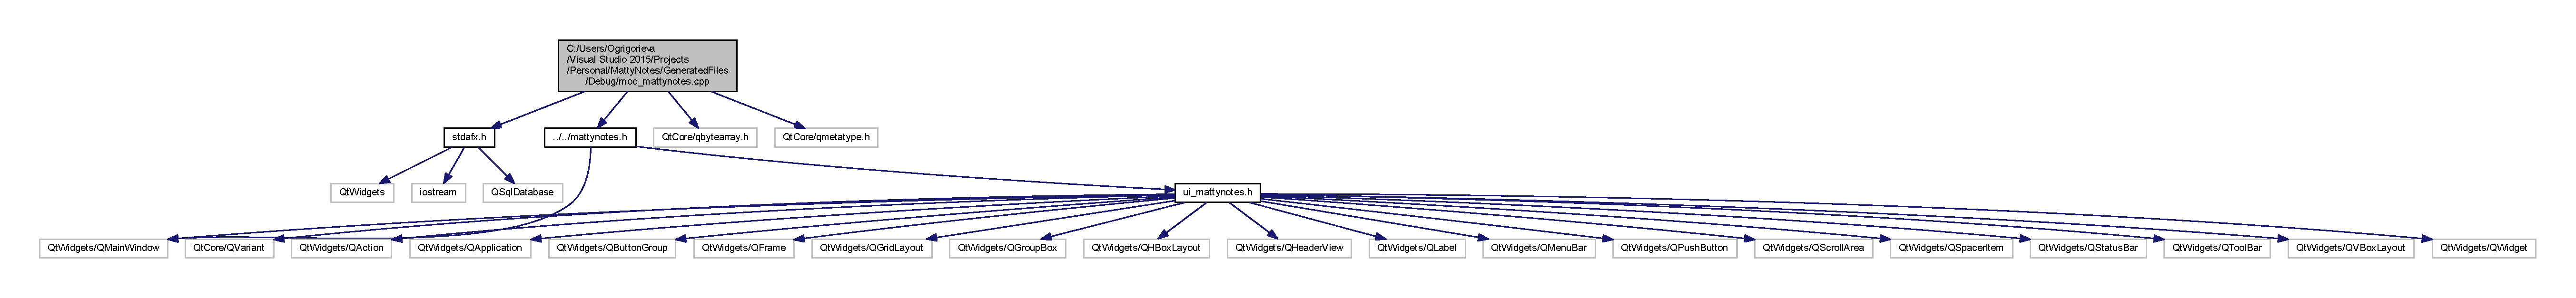
\includegraphics[width=350pt]{Debug_2moc__mattynotes_8cpp__incl}
\end{center}
\end{figure}
\subsection*{Classes}
\begin{DoxyCompactItemize}
\item 
struct \hyperlink{structqt__meta__stringdata__MattyNotes__t}{qt\+\_\+meta\+\_\+stringdata\+\_\+\+Matty\+Notes\+\_\+t}
\end{DoxyCompactItemize}
\subsection*{Macros}
\begin{DoxyCompactItemize}
\item 
\#define \hyperlink{Debug_2moc__mattynotes_8cpp_a75bb9482d242cde0a06c9dbdc6b83abe}{Q\+T\+\_\+\+M\+O\+C\+\_\+\+L\+I\+T\+E\+R\+AL}(idx,  ofs,  len)
\end{DoxyCompactItemize}
\subsection*{Variables}
\begin{DoxyCompactItemize}
\item 
static const \hyperlink{structqt__meta__stringdata__MattyNotes__t}{qt\+\_\+meta\+\_\+stringdata\+\_\+\+Matty\+Notes\+\_\+t} \hyperlink{Debug_2moc__mattynotes_8cpp_a1be372cf600bc7b2eb61145bea6fcb41}{qt\+\_\+meta\+\_\+stringdata\+\_\+\+Matty\+Notes}
\item 
static const uint \hyperlink{Debug_2moc__mattynotes_8cpp_a5b99b001af52ab97154d3fd2373c4477}{qt\+\_\+meta\+\_\+data\+\_\+\+Matty\+Notes} \mbox{[}$\,$\mbox{]}
\end{DoxyCompactItemize}


\subsection{Macro Definition Documentation}
\hypertarget{Debug_2moc__mattynotes_8cpp_a75bb9482d242cde0a06c9dbdc6b83abe}{}\label{Debug_2moc__mattynotes_8cpp_a75bb9482d242cde0a06c9dbdc6b83abe} 
\index{Debug/moc\+\_\+mattynotes.\+cpp@{Debug/moc\+\_\+mattynotes.\+cpp}!Q\+T\+\_\+\+M\+O\+C\+\_\+\+L\+I\+T\+E\+R\+AL@{Q\+T\+\_\+\+M\+O\+C\+\_\+\+L\+I\+T\+E\+R\+AL}}
\index{Q\+T\+\_\+\+M\+O\+C\+\_\+\+L\+I\+T\+E\+R\+AL@{Q\+T\+\_\+\+M\+O\+C\+\_\+\+L\+I\+T\+E\+R\+AL}!Debug/moc\+\_\+mattynotes.\+cpp@{Debug/moc\+\_\+mattynotes.\+cpp}}
\subsubsection{\texorpdfstring{Q\+T\+\_\+\+M\+O\+C\+\_\+\+L\+I\+T\+E\+R\+AL}{QT\_MOC\_LITERAL}}
{\footnotesize\ttfamily \#define Q\+T\+\_\+\+M\+O\+C\+\_\+\+L\+I\+T\+E\+R\+AL(\begin{DoxyParamCaption}\item[{}]{idx,  }\item[{}]{ofs,  }\item[{}]{len }\end{DoxyParamCaption})}

{\bfseries Value\+:}
\begin{DoxyCode}
Q\_STATIC\_BYTE\_ARRAY\_DATA\_HEADER\_INITIALIZER\_WITH\_OFFSET(len, \(\backslash\)
    qptrdiff(offsetof(\hyperlink{structqt__meta__stringdata__MattyNotes__t}{qt\_meta\_stringdata\_MattyNotes\_t}, stringdata0) + ofs \(\backslash\)
        - idx * \textcolor{keyword}{sizeof}(QByteArrayData)) \(\backslash\)
    )
\end{DoxyCode}


Definition at line 26 of file moc\+\_\+mattynotes.\+cpp.



\subsection{Variable Documentation}
\hypertarget{Debug_2moc__mattynotes_8cpp_a5b99b001af52ab97154d3fd2373c4477}{}\label{Debug_2moc__mattynotes_8cpp_a5b99b001af52ab97154d3fd2373c4477} 
\index{Debug/moc\+\_\+mattynotes.\+cpp@{Debug/moc\+\_\+mattynotes.\+cpp}!qt\+\_\+meta\+\_\+data\+\_\+\+Matty\+Notes@{qt\+\_\+meta\+\_\+data\+\_\+\+Matty\+Notes}}
\index{qt\+\_\+meta\+\_\+data\+\_\+\+Matty\+Notes@{qt\+\_\+meta\+\_\+data\+\_\+\+Matty\+Notes}!Debug/moc\+\_\+mattynotes.\+cpp@{Debug/moc\+\_\+mattynotes.\+cpp}}
\subsubsection{\texorpdfstring{qt\+\_\+meta\+\_\+data\+\_\+\+Matty\+Notes}{qt\_meta\_data\_MattyNotes}}
{\footnotesize\ttfamily const uint qt\+\_\+meta\+\_\+data\+\_\+\+Matty\+Notes\mbox{[}$\,$\mbox{]}\hspace{0.3cm}{\ttfamily [static]}}

{\bfseries Initial value\+:}
\begin{DoxyCode}
= \{

 
       7,       
       0,       
       0,    0, 
       4,   14, 
       0,    0, 
       0,    0, 
       0,    0, 
       0,       
       0,       

 
       1,    0,   34,    2, 0x08 ,
       3,    0,   35,    2, 0x08 ,
       4,    0,   36,    2, 0x08 ,
       5,    0,   37,    2, 0x08 ,

 
    QMetaType::Void,
    QMetaType::Void,
    QMetaType::Void,
    QMetaType::Void,

       0        
\}
\end{DoxyCode}


Definition at line 46 of file moc\+\_\+mattynotes.\+cpp.

\hypertarget{Debug_2moc__mattynotes_8cpp_a1be372cf600bc7b2eb61145bea6fcb41}{}\label{Debug_2moc__mattynotes_8cpp_a1be372cf600bc7b2eb61145bea6fcb41} 
\index{Debug/moc\+\_\+mattynotes.\+cpp@{Debug/moc\+\_\+mattynotes.\+cpp}!qt\+\_\+meta\+\_\+stringdata\+\_\+\+Matty\+Notes@{qt\+\_\+meta\+\_\+stringdata\+\_\+\+Matty\+Notes}}
\index{qt\+\_\+meta\+\_\+stringdata\+\_\+\+Matty\+Notes@{qt\+\_\+meta\+\_\+stringdata\+\_\+\+Matty\+Notes}!Debug/moc\+\_\+mattynotes.\+cpp@{Debug/moc\+\_\+mattynotes.\+cpp}}
\subsubsection{\texorpdfstring{qt\+\_\+meta\+\_\+stringdata\+\_\+\+Matty\+Notes}{qt\_meta\_stringdata\_MattyNotes}}
{\footnotesize\ttfamily const \hyperlink{structqt__meta__stringdata__MattyNotes__t}{qt\+\_\+meta\+\_\+stringdata\+\_\+\+Matty\+Notes\+\_\+t} qt\+\_\+meta\+\_\+stringdata\+\_\+\+Matty\+Notes\hspace{0.3cm}{\ttfamily [static]}}

{\bfseries Initial value\+:}
\begin{DoxyCode}
= \{
    \{
\hyperlink{Debug_2moc__mattynotes_8cpp_a75bb9482d242cde0a06c9dbdc6b83abe}{QT\_MOC\_LITERAL}(0, 0, 10), 
\hyperlink{Debug_2moc__mattynotes_8cpp_a75bb9482d242cde0a06c9dbdc6b83abe}{QT\_MOC\_LITERAL}(1, 11, 28), 
\hyperlink{Debug_2moc__mattynotes_8cpp_a75bb9482d242cde0a06c9dbdc6b83abe}{QT\_MOC\_LITERAL}(2, 40, 0), 
\hyperlink{Debug_2moc__mattynotes_8cpp_a75bb9482d242cde0a06c9dbdc6b83abe}{QT\_MOC\_LITERAL}(3, 41, 11), 
\hyperlink{Debug_2moc__mattynotes_8cpp_a75bb9482d242cde0a06c9dbdc6b83abe}{QT\_MOC\_LITERAL}(4, 53, 14), 
\hyperlink{Debug_2moc__mattynotes_8cpp_a75bb9482d242cde0a06c9dbdc6b83abe}{QT\_MOC\_LITERAL}(5, 68, 14) 

    \},
    \textcolor{stringliteral}{"MattyNotes\(\backslash\)0on\_addNoteButtonTemp\_clicked\(\backslash\)0"}
    \textcolor{stringliteral}{"\(\backslash\)0closeWindow\(\backslash\)0maximizeWindow\(\backslash\)0minimizeWindow"}
\}
\end{DoxyCode}


Definition at line 31 of file moc\+\_\+mattynotes.\+cpp.


\hypertarget{Release_2moc__mattynotes_8cpp}{}\section{C\+:/\+Users/\+Ogrigorieva/\+Visual Studio 2015/\+Projects/\+Personal/\+Matty\+Notes/\+Generated\+Files/\+Release/moc\+\_\+mattynotes.cpp File Reference}
\label{Release_2moc__mattynotes_8cpp}\index{C\+:/\+Users/\+Ogrigorieva/\+Visual Studio 2015/\+Projects/\+Personal/\+Matty\+Notes/\+Generated\+Files/\+Release/moc\+\_\+mattynotes.\+cpp@{C\+:/\+Users/\+Ogrigorieva/\+Visual Studio 2015/\+Projects/\+Personal/\+Matty\+Notes/\+Generated\+Files/\+Release/moc\+\_\+mattynotes.\+cpp}}
{\ttfamily \#include \char`\"{}stdafx.\+h\char`\"{}}\newline
{\ttfamily \#include \char`\"{}../../mattynotes.\+h\char`\"{}}\newline
{\ttfamily \#include $<$Qt\+Core/qbytearray.\+h$>$}\newline
{\ttfamily \#include $<$Qt\+Core/qmetatype.\+h$>$}\newline
Include dependency graph for moc\+\_\+mattynotes.\+cpp\+:
\nopagebreak
\begin{figure}[H]
\begin{center}
\leavevmode
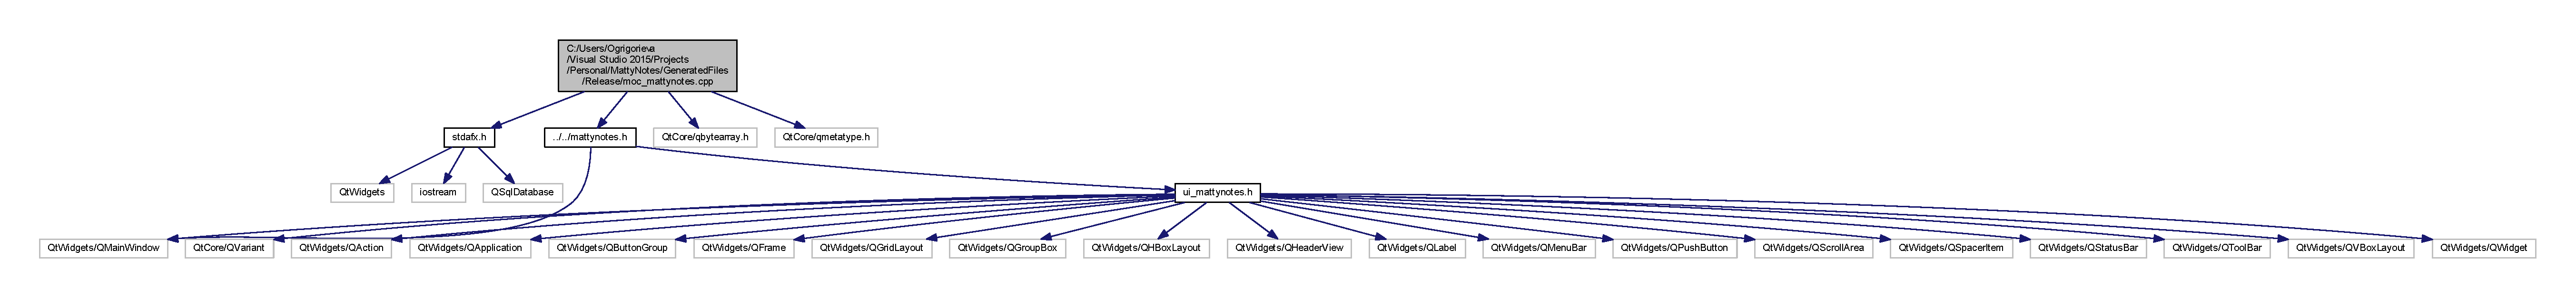
\includegraphics[width=350pt]{Release_2moc__mattynotes_8cpp__incl}
\end{center}
\end{figure}
\subsection*{Classes}
\begin{DoxyCompactItemize}
\item 
struct \hyperlink{structqt__meta__stringdata__MattyNotes__t}{qt\+\_\+meta\+\_\+stringdata\+\_\+\+Matty\+Notes\+\_\+t}
\end{DoxyCompactItemize}
\subsection*{Macros}
\begin{DoxyCompactItemize}
\item 
\#define \hyperlink{Release_2moc__mattynotes_8cpp_a75bb9482d242cde0a06c9dbdc6b83abe}{Q\+T\+\_\+\+M\+O\+C\+\_\+\+L\+I\+T\+E\+R\+AL}(idx,  ofs,  len)
\end{DoxyCompactItemize}
\subsection*{Variables}
\begin{DoxyCompactItemize}
\item 
static const \hyperlink{structqt__meta__stringdata__MattyNotes__t}{qt\+\_\+meta\+\_\+stringdata\+\_\+\+Matty\+Notes\+\_\+t} \hyperlink{Release_2moc__mattynotes_8cpp_a1be372cf600bc7b2eb61145bea6fcb41}{qt\+\_\+meta\+\_\+stringdata\+\_\+\+Matty\+Notes}
\item 
static const uint \hyperlink{Release_2moc__mattynotes_8cpp_a5b99b001af52ab97154d3fd2373c4477}{qt\+\_\+meta\+\_\+data\+\_\+\+Matty\+Notes} \mbox{[}$\,$\mbox{]}
\end{DoxyCompactItemize}


\subsection{Macro Definition Documentation}
\hypertarget{Release_2moc__mattynotes_8cpp_a75bb9482d242cde0a06c9dbdc6b83abe}{}\label{Release_2moc__mattynotes_8cpp_a75bb9482d242cde0a06c9dbdc6b83abe} 
\index{Release/moc\+\_\+mattynotes.\+cpp@{Release/moc\+\_\+mattynotes.\+cpp}!Q\+T\+\_\+\+M\+O\+C\+\_\+\+L\+I\+T\+E\+R\+AL@{Q\+T\+\_\+\+M\+O\+C\+\_\+\+L\+I\+T\+E\+R\+AL}}
\index{Q\+T\+\_\+\+M\+O\+C\+\_\+\+L\+I\+T\+E\+R\+AL@{Q\+T\+\_\+\+M\+O\+C\+\_\+\+L\+I\+T\+E\+R\+AL}!Release/moc\+\_\+mattynotes.\+cpp@{Release/moc\+\_\+mattynotes.\+cpp}}
\subsubsection{\texorpdfstring{Q\+T\+\_\+\+M\+O\+C\+\_\+\+L\+I\+T\+E\+R\+AL}{QT\_MOC\_LITERAL}}
{\footnotesize\ttfamily \#define Q\+T\+\_\+\+M\+O\+C\+\_\+\+L\+I\+T\+E\+R\+AL(\begin{DoxyParamCaption}\item[{}]{idx,  }\item[{}]{ofs,  }\item[{}]{len }\end{DoxyParamCaption})}

{\bfseries Value\+:}
\begin{DoxyCode}
Q\_STATIC\_BYTE\_ARRAY\_DATA\_HEADER\_INITIALIZER\_WITH\_OFFSET(len, \(\backslash\)
    qptrdiff(offsetof(\hyperlink{structqt__meta__stringdata__MattyNotes__t}{qt\_meta\_stringdata\_MattyNotes\_t}, stringdata0) + ofs \(\backslash\)
        - idx * \textcolor{keyword}{sizeof}(QByteArrayData)) \(\backslash\)
    )
\end{DoxyCode}


Definition at line 26 of file moc\+\_\+mattynotes.\+cpp.



\subsection{Variable Documentation}
\hypertarget{Release_2moc__mattynotes_8cpp_a5b99b001af52ab97154d3fd2373c4477}{}\label{Release_2moc__mattynotes_8cpp_a5b99b001af52ab97154d3fd2373c4477} 
\index{Release/moc\+\_\+mattynotes.\+cpp@{Release/moc\+\_\+mattynotes.\+cpp}!qt\+\_\+meta\+\_\+data\+\_\+\+Matty\+Notes@{qt\+\_\+meta\+\_\+data\+\_\+\+Matty\+Notes}}
\index{qt\+\_\+meta\+\_\+data\+\_\+\+Matty\+Notes@{qt\+\_\+meta\+\_\+data\+\_\+\+Matty\+Notes}!Release/moc\+\_\+mattynotes.\+cpp@{Release/moc\+\_\+mattynotes.\+cpp}}
\subsubsection{\texorpdfstring{qt\+\_\+meta\+\_\+data\+\_\+\+Matty\+Notes}{qt\_meta\_data\_MattyNotes}}
{\footnotesize\ttfamily const uint qt\+\_\+meta\+\_\+data\+\_\+\+Matty\+Notes\mbox{[}$\,$\mbox{]}\hspace{0.3cm}{\ttfamily [static]}}

{\bfseries Initial value\+:}
\begin{DoxyCode}
= \{

 
       7,       
       0,       
       0,    0, 
       4,   14, 
       0,    0, 
       0,    0, 
       0,    0, 
       0,       
       0,       

 
       1,    0,   34,    2, 0x08 ,
       3,    0,   35,    2, 0x08 ,
       4,    0,   36,    2, 0x08 ,
       5,    0,   37,    2, 0x08 ,

 
    QMetaType::Void,
    QMetaType::Void,
    QMetaType::Void,
    QMetaType::Void,

       0        
\}
\end{DoxyCode}


Definition at line 46 of file moc\+\_\+mattynotes.\+cpp.

\hypertarget{Release_2moc__mattynotes_8cpp_a1be372cf600bc7b2eb61145bea6fcb41}{}\label{Release_2moc__mattynotes_8cpp_a1be372cf600bc7b2eb61145bea6fcb41} 
\index{Release/moc\+\_\+mattynotes.\+cpp@{Release/moc\+\_\+mattynotes.\+cpp}!qt\+\_\+meta\+\_\+stringdata\+\_\+\+Matty\+Notes@{qt\+\_\+meta\+\_\+stringdata\+\_\+\+Matty\+Notes}}
\index{qt\+\_\+meta\+\_\+stringdata\+\_\+\+Matty\+Notes@{qt\+\_\+meta\+\_\+stringdata\+\_\+\+Matty\+Notes}!Release/moc\+\_\+mattynotes.\+cpp@{Release/moc\+\_\+mattynotes.\+cpp}}
\subsubsection{\texorpdfstring{qt\+\_\+meta\+\_\+stringdata\+\_\+\+Matty\+Notes}{qt\_meta\_stringdata\_MattyNotes}}
{\footnotesize\ttfamily const \hyperlink{structqt__meta__stringdata__MattyNotes__t}{qt\+\_\+meta\+\_\+stringdata\+\_\+\+Matty\+Notes\+\_\+t} qt\+\_\+meta\+\_\+stringdata\+\_\+\+Matty\+Notes\hspace{0.3cm}{\ttfamily [static]}}

{\bfseries Initial value\+:}
\begin{DoxyCode}
= \{
    \{
\hyperlink{Release_2moc__mattynotes_8cpp_a75bb9482d242cde0a06c9dbdc6b83abe}{QT\_MOC\_LITERAL}(0, 0, 10), 
\hyperlink{Release_2moc__mattynotes_8cpp_a75bb9482d242cde0a06c9dbdc6b83abe}{QT\_MOC\_LITERAL}(1, 11, 28), 
\hyperlink{Release_2moc__mattynotes_8cpp_a75bb9482d242cde0a06c9dbdc6b83abe}{QT\_MOC\_LITERAL}(2, 40, 0), 
\hyperlink{Release_2moc__mattynotes_8cpp_a75bb9482d242cde0a06c9dbdc6b83abe}{QT\_MOC\_LITERAL}(3, 41, 11), 
\hyperlink{Release_2moc__mattynotes_8cpp_a75bb9482d242cde0a06c9dbdc6b83abe}{QT\_MOC\_LITERAL}(4, 53, 14), 
\hyperlink{Release_2moc__mattynotes_8cpp_a75bb9482d242cde0a06c9dbdc6b83abe}{QT\_MOC\_LITERAL}(5, 68, 14) 

    \},
    \textcolor{stringliteral}{"MattyNotes\(\backslash\)0on\_addNoteButtonTemp\_clicked\(\backslash\)0"}
    \textcolor{stringliteral}{"\(\backslash\)0closeWindow\(\backslash\)0maximizeWindow\(\backslash\)0minimizeWindow"}
\}
\end{DoxyCode}


Definition at line 31 of file moc\+\_\+mattynotes.\+cpp.


\hypertarget{Debug_2moc__mattysettings_8cpp}{}\section{C\+:/\+Users/\+Ogrigorieva/\+Visual Studio 2015/\+Projects/\+Personal/\+Matty\+Notes/\+Generated\+Files/\+Debug/moc\+\_\+mattysettings.cpp File Reference}
\label{Debug_2moc__mattysettings_8cpp}\index{C\+:/\+Users/\+Ogrigorieva/\+Visual Studio 2015/\+Projects/\+Personal/\+Matty\+Notes/\+Generated\+Files/\+Debug/moc\+\_\+mattysettings.\+cpp@{C\+:/\+Users/\+Ogrigorieva/\+Visual Studio 2015/\+Projects/\+Personal/\+Matty\+Notes/\+Generated\+Files/\+Debug/moc\+\_\+mattysettings.\+cpp}}
{\ttfamily \#include \char`\"{}stdafx.\+h\char`\"{}}\newline
{\ttfamily \#include \char`\"{}../../mattysettings.\+h\char`\"{}}\newline
{\ttfamily \#include $<$Qt\+Core/qbytearray.\+h$>$}\newline
{\ttfamily \#include $<$Qt\+Core/qmetatype.\+h$>$}\newline
Include dependency graph for moc\+\_\+mattysettings.\+cpp\+:
\nopagebreak
\begin{figure}[H]
\begin{center}
\leavevmode
\includegraphics[width=350pt]{Debug_2moc__mattysettings_8cpp__incl}
\end{center}
\end{figure}
\subsection*{Classes}
\begin{DoxyCompactItemize}
\item 
struct \hyperlink{structqt__meta__stringdata__MattySettings__t}{qt\+\_\+meta\+\_\+stringdata\+\_\+\+Matty\+Settings\+\_\+t}
\end{DoxyCompactItemize}
\subsection*{Macros}
\begin{DoxyCompactItemize}
\item 
\#define \hyperlink{Debug_2moc__mattysettings_8cpp_a75bb9482d242cde0a06c9dbdc6b83abe}{Q\+T\+\_\+\+M\+O\+C\+\_\+\+L\+I\+T\+E\+R\+AL}(idx,  ofs,  len)
\end{DoxyCompactItemize}
\subsection*{Variables}
\begin{DoxyCompactItemize}
\item 
static const \hyperlink{structqt__meta__stringdata__MattySettings__t}{qt\+\_\+meta\+\_\+stringdata\+\_\+\+Matty\+Settings\+\_\+t} \hyperlink{Debug_2moc__mattysettings_8cpp_aa76912f00626d44ffa539f92621adada}{qt\+\_\+meta\+\_\+stringdata\+\_\+\+Matty\+Settings}
\item 
static const uint \hyperlink{Debug_2moc__mattysettings_8cpp_a65b41b7e18b1055f39bb3e7dfcc3cc2b}{qt\+\_\+meta\+\_\+data\+\_\+\+Matty\+Settings} \mbox{[}$\,$\mbox{]}
\end{DoxyCompactItemize}


\subsection{Macro Definition Documentation}
\hypertarget{Debug_2moc__mattysettings_8cpp_a75bb9482d242cde0a06c9dbdc6b83abe}{}\label{Debug_2moc__mattysettings_8cpp_a75bb9482d242cde0a06c9dbdc6b83abe} 
\index{Debug/moc\+\_\+mattysettings.\+cpp@{Debug/moc\+\_\+mattysettings.\+cpp}!Q\+T\+\_\+\+M\+O\+C\+\_\+\+L\+I\+T\+E\+R\+AL@{Q\+T\+\_\+\+M\+O\+C\+\_\+\+L\+I\+T\+E\+R\+AL}}
\index{Q\+T\+\_\+\+M\+O\+C\+\_\+\+L\+I\+T\+E\+R\+AL@{Q\+T\+\_\+\+M\+O\+C\+\_\+\+L\+I\+T\+E\+R\+AL}!Debug/moc\+\_\+mattysettings.\+cpp@{Debug/moc\+\_\+mattysettings.\+cpp}}
\subsubsection{\texorpdfstring{Q\+T\+\_\+\+M\+O\+C\+\_\+\+L\+I\+T\+E\+R\+AL}{QT\_MOC\_LITERAL}}
{\footnotesize\ttfamily \#define Q\+T\+\_\+\+M\+O\+C\+\_\+\+L\+I\+T\+E\+R\+AL(\begin{DoxyParamCaption}\item[{}]{idx,  }\item[{}]{ofs,  }\item[{}]{len }\end{DoxyParamCaption})}

{\bfseries Value\+:}
\begin{DoxyCode}
Q\_STATIC\_BYTE\_ARRAY\_DATA\_HEADER\_INITIALIZER\_WITH\_OFFSET(len, \(\backslash\)
    qptrdiff(offsetof(\hyperlink{structqt__meta__stringdata__MattySettings__t}{qt\_meta\_stringdata\_MattySettings\_t}, stringdata0) + 
      ofs \(\backslash\)
        - idx * \textcolor{keyword}{sizeof}(QByteArrayData)) \(\backslash\)
    )
\end{DoxyCode}


Definition at line 26 of file moc\+\_\+mattysettings.\+cpp.



\subsection{Variable Documentation}
\hypertarget{Debug_2moc__mattysettings_8cpp_a65b41b7e18b1055f39bb3e7dfcc3cc2b}{}\label{Debug_2moc__mattysettings_8cpp_a65b41b7e18b1055f39bb3e7dfcc3cc2b} 
\index{Debug/moc\+\_\+mattysettings.\+cpp@{Debug/moc\+\_\+mattysettings.\+cpp}!qt\+\_\+meta\+\_\+data\+\_\+\+Matty\+Settings@{qt\+\_\+meta\+\_\+data\+\_\+\+Matty\+Settings}}
\index{qt\+\_\+meta\+\_\+data\+\_\+\+Matty\+Settings@{qt\+\_\+meta\+\_\+data\+\_\+\+Matty\+Settings}!Debug/moc\+\_\+mattysettings.\+cpp@{Debug/moc\+\_\+mattysettings.\+cpp}}
\subsubsection{\texorpdfstring{qt\+\_\+meta\+\_\+data\+\_\+\+Matty\+Settings}{qt\_meta\_data\_MattySettings}}
{\footnotesize\ttfamily const uint qt\+\_\+meta\+\_\+data\+\_\+\+Matty\+Settings\mbox{[}$\,$\mbox{]}\hspace{0.3cm}{\ttfamily [static]}}

{\bfseries Initial value\+:}
\begin{DoxyCode}
= \{

 
       7,       
       0,       
       0,    0, 
       0,    0, 
       0,    0, 
       0,    0, 
       0,    0, 
       0,       
       0,       

       0        
\}
\end{DoxyCode}


Definition at line 40 of file moc\+\_\+mattysettings.\+cpp.

\hypertarget{Debug_2moc__mattysettings_8cpp_aa76912f00626d44ffa539f92621adada}{}\label{Debug_2moc__mattysettings_8cpp_aa76912f00626d44ffa539f92621adada} 
\index{Debug/moc\+\_\+mattysettings.\+cpp@{Debug/moc\+\_\+mattysettings.\+cpp}!qt\+\_\+meta\+\_\+stringdata\+\_\+\+Matty\+Settings@{qt\+\_\+meta\+\_\+stringdata\+\_\+\+Matty\+Settings}}
\index{qt\+\_\+meta\+\_\+stringdata\+\_\+\+Matty\+Settings@{qt\+\_\+meta\+\_\+stringdata\+\_\+\+Matty\+Settings}!Debug/moc\+\_\+mattysettings.\+cpp@{Debug/moc\+\_\+mattysettings.\+cpp}}
\subsubsection{\texorpdfstring{qt\+\_\+meta\+\_\+stringdata\+\_\+\+Matty\+Settings}{qt\_meta\_stringdata\_MattySettings}}
{\footnotesize\ttfamily const \hyperlink{structqt__meta__stringdata__MattySettings__t}{qt\+\_\+meta\+\_\+stringdata\+\_\+\+Matty\+Settings\+\_\+t} qt\+\_\+meta\+\_\+stringdata\+\_\+\+Matty\+Settings\hspace{0.3cm}{\ttfamily [static]}}

{\bfseries Initial value\+:}
\begin{DoxyCode}
= \{
    \{
\hyperlink{Debug_2moc__mattysettings_8cpp_a75bb9482d242cde0a06c9dbdc6b83abe}{QT\_MOC\_LITERAL}(0, 0, 13) 

    \},
    \textcolor{stringliteral}{"MattySettings"}
\}
\end{DoxyCode}


Definition at line 31 of file moc\+\_\+mattysettings.\+cpp.


\hypertarget{Release_2moc__mattysettings_8cpp}{}\section{C\+:/\+Users/\+Ogrigorieva/\+Visual Studio 2015/\+Projects/\+Personal/\+Matty\+Notes/\+Generated\+Files/\+Release/moc\+\_\+mattysettings.cpp File Reference}
\label{Release_2moc__mattysettings_8cpp}\index{C\+:/\+Users/\+Ogrigorieva/\+Visual Studio 2015/\+Projects/\+Personal/\+Matty\+Notes/\+Generated\+Files/\+Release/moc\+\_\+mattysettings.\+cpp@{C\+:/\+Users/\+Ogrigorieva/\+Visual Studio 2015/\+Projects/\+Personal/\+Matty\+Notes/\+Generated\+Files/\+Release/moc\+\_\+mattysettings.\+cpp}}
{\ttfamily \#include \char`\"{}stdafx.\+h\char`\"{}}\newline
{\ttfamily \#include \char`\"{}../../mattysettings.\+h\char`\"{}}\newline
{\ttfamily \#include $<$Qt\+Core/qbytearray.\+h$>$}\newline
{\ttfamily \#include $<$Qt\+Core/qmetatype.\+h$>$}\newline
Include dependency graph for moc\+\_\+mattysettings.\+cpp\+:
\nopagebreak
\begin{figure}[H]
\begin{center}
\leavevmode
\includegraphics[width=350pt]{Release_2moc__mattysettings_8cpp__incl}
\end{center}
\end{figure}
\subsection*{Classes}
\begin{DoxyCompactItemize}
\item 
struct \hyperlink{structqt__meta__stringdata__MattySettings__t}{qt\+\_\+meta\+\_\+stringdata\+\_\+\+Matty\+Settings\+\_\+t}
\end{DoxyCompactItemize}
\subsection*{Macros}
\begin{DoxyCompactItemize}
\item 
\#define \hyperlink{Release_2moc__mattysettings_8cpp_a75bb9482d242cde0a06c9dbdc6b83abe}{Q\+T\+\_\+\+M\+O\+C\+\_\+\+L\+I\+T\+E\+R\+AL}(idx,  ofs,  len)
\end{DoxyCompactItemize}
\subsection*{Variables}
\begin{DoxyCompactItemize}
\item 
static const \hyperlink{structqt__meta__stringdata__MattySettings__t}{qt\+\_\+meta\+\_\+stringdata\+\_\+\+Matty\+Settings\+\_\+t} \hyperlink{Release_2moc__mattysettings_8cpp_aa76912f00626d44ffa539f92621adada}{qt\+\_\+meta\+\_\+stringdata\+\_\+\+Matty\+Settings}
\item 
static const uint \hyperlink{Release_2moc__mattysettings_8cpp_a65b41b7e18b1055f39bb3e7dfcc3cc2b}{qt\+\_\+meta\+\_\+data\+\_\+\+Matty\+Settings} \mbox{[}$\,$\mbox{]}
\end{DoxyCompactItemize}


\subsection{Macro Definition Documentation}
\hypertarget{Release_2moc__mattysettings_8cpp_a75bb9482d242cde0a06c9dbdc6b83abe}{}\label{Release_2moc__mattysettings_8cpp_a75bb9482d242cde0a06c9dbdc6b83abe} 
\index{Release/moc\+\_\+mattysettings.\+cpp@{Release/moc\+\_\+mattysettings.\+cpp}!Q\+T\+\_\+\+M\+O\+C\+\_\+\+L\+I\+T\+E\+R\+AL@{Q\+T\+\_\+\+M\+O\+C\+\_\+\+L\+I\+T\+E\+R\+AL}}
\index{Q\+T\+\_\+\+M\+O\+C\+\_\+\+L\+I\+T\+E\+R\+AL@{Q\+T\+\_\+\+M\+O\+C\+\_\+\+L\+I\+T\+E\+R\+AL}!Release/moc\+\_\+mattysettings.\+cpp@{Release/moc\+\_\+mattysettings.\+cpp}}
\subsubsection{\texorpdfstring{Q\+T\+\_\+\+M\+O\+C\+\_\+\+L\+I\+T\+E\+R\+AL}{QT\_MOC\_LITERAL}}
{\footnotesize\ttfamily \#define Q\+T\+\_\+\+M\+O\+C\+\_\+\+L\+I\+T\+E\+R\+AL(\begin{DoxyParamCaption}\item[{}]{idx,  }\item[{}]{ofs,  }\item[{}]{len }\end{DoxyParamCaption})}

{\bfseries Value\+:}
\begin{DoxyCode}
Q\_STATIC\_BYTE\_ARRAY\_DATA\_HEADER\_INITIALIZER\_WITH\_OFFSET(len, \(\backslash\)
    qptrdiff(offsetof(\hyperlink{structqt__meta__stringdata__MattySettings__t}{qt\_meta\_stringdata\_MattySettings\_t}, stringdata0) + 
      ofs \(\backslash\)
        - idx * \textcolor{keyword}{sizeof}(QByteArrayData)) \(\backslash\)
    )
\end{DoxyCode}


Definition at line 26 of file moc\+\_\+mattysettings.\+cpp.



\subsection{Variable Documentation}
\hypertarget{Release_2moc__mattysettings_8cpp_a65b41b7e18b1055f39bb3e7dfcc3cc2b}{}\label{Release_2moc__mattysettings_8cpp_a65b41b7e18b1055f39bb3e7dfcc3cc2b} 
\index{Release/moc\+\_\+mattysettings.\+cpp@{Release/moc\+\_\+mattysettings.\+cpp}!qt\+\_\+meta\+\_\+data\+\_\+\+Matty\+Settings@{qt\+\_\+meta\+\_\+data\+\_\+\+Matty\+Settings}}
\index{qt\+\_\+meta\+\_\+data\+\_\+\+Matty\+Settings@{qt\+\_\+meta\+\_\+data\+\_\+\+Matty\+Settings}!Release/moc\+\_\+mattysettings.\+cpp@{Release/moc\+\_\+mattysettings.\+cpp}}
\subsubsection{\texorpdfstring{qt\+\_\+meta\+\_\+data\+\_\+\+Matty\+Settings}{qt\_meta\_data\_MattySettings}}
{\footnotesize\ttfamily const uint qt\+\_\+meta\+\_\+data\+\_\+\+Matty\+Settings\mbox{[}$\,$\mbox{]}\hspace{0.3cm}{\ttfamily [static]}}

{\bfseries Initial value\+:}
\begin{DoxyCode}
= \{

 
       7,       
       0,       
       0,    0, 
       0,    0, 
       0,    0, 
       0,    0, 
       0,    0, 
       0,       
       0,       

       0        
\}
\end{DoxyCode}


Definition at line 40 of file moc\+\_\+mattysettings.\+cpp.

\hypertarget{Release_2moc__mattysettings_8cpp_aa76912f00626d44ffa539f92621adada}{}\label{Release_2moc__mattysettings_8cpp_aa76912f00626d44ffa539f92621adada} 
\index{Release/moc\+\_\+mattysettings.\+cpp@{Release/moc\+\_\+mattysettings.\+cpp}!qt\+\_\+meta\+\_\+stringdata\+\_\+\+Matty\+Settings@{qt\+\_\+meta\+\_\+stringdata\+\_\+\+Matty\+Settings}}
\index{qt\+\_\+meta\+\_\+stringdata\+\_\+\+Matty\+Settings@{qt\+\_\+meta\+\_\+stringdata\+\_\+\+Matty\+Settings}!Release/moc\+\_\+mattysettings.\+cpp@{Release/moc\+\_\+mattysettings.\+cpp}}
\subsubsection{\texorpdfstring{qt\+\_\+meta\+\_\+stringdata\+\_\+\+Matty\+Settings}{qt\_meta\_stringdata\_MattySettings}}
{\footnotesize\ttfamily const \hyperlink{structqt__meta__stringdata__MattySettings__t}{qt\+\_\+meta\+\_\+stringdata\+\_\+\+Matty\+Settings\+\_\+t} qt\+\_\+meta\+\_\+stringdata\+\_\+\+Matty\+Settings\hspace{0.3cm}{\ttfamily [static]}}

{\bfseries Initial value\+:}
\begin{DoxyCode}
= \{
    \{
\hyperlink{Release_2moc__mattysettings_8cpp_a75bb9482d242cde0a06c9dbdc6b83abe}{QT\_MOC\_LITERAL}(0, 0, 13) 

    \},
    \textcolor{stringliteral}{"MattySettings"}
\}
\end{DoxyCode}


Definition at line 31 of file moc\+\_\+mattysettings.\+cpp.


\hypertarget{qrc__mattynotes_8cpp}{}\section{C\+:/\+Users/\+Ogrigorieva/\+Visual Studio 2015/\+Projects/\+Personal/\+Matty\+Notes/\+Generated\+Files/qrc\+\_\+mattynotes.cpp File Reference}
\label{qrc__mattynotes_8cpp}\index{C\+:/\+Users/\+Ogrigorieva/\+Visual Studio 2015/\+Projects/\+Personal/\+Matty\+Notes/\+Generated\+Files/qrc\+\_\+mattynotes.\+cpp@{C\+:/\+Users/\+Ogrigorieva/\+Visual Studio 2015/\+Projects/\+Personal/\+Matty\+Notes/\+Generated\+Files/qrc\+\_\+mattynotes.\+cpp}}
\subsection*{Macros}
\begin{DoxyCompactItemize}
\item 
\#define \hyperlink{qrc__mattynotes_8cpp_afbfc3bb3cd2fa03dd0a3fc36563480d6}{Q\+T\+\_\+\+R\+C\+C\+\_\+\+P\+R\+E\+P\+E\+N\+D\+\_\+\+N\+A\+M\+E\+S\+P\+A\+CE}(name)~name
\item 
\#define \hyperlink{qrc__mattynotes_8cpp_a590f80ddb226779f6f432d80438ea190}{Q\+T\+\_\+\+R\+C\+C\+\_\+\+M\+A\+N\+G\+L\+E\+\_\+\+N\+A\+M\+E\+S\+P\+A\+CE}(name)~name
\end{DoxyCompactItemize}
\subsection*{Functions}
\begin{DoxyCompactItemize}
\item 
bool \hyperlink{qrc__mattynotes_8cpp_a2ce5a6cde5b318dc75442940471e05f7}{q\+Register\+Resource\+Data} (int, const unsigned char $\ast$, const unsigned char $\ast$, const unsigned char $\ast$)
\item 
bool \hyperlink{qrc__mattynotes_8cpp_a54b96c9f44d004fc0ea13bb581f97a71}{q\+Unregister\+Resource\+Data} (int, const unsigned char $\ast$, const unsigned char $\ast$, const unsigned char $\ast$)
\item 
int \hyperlink{qrc__mattynotes_8cpp_a590f80ddb226779f6f432d80438ea190}{Q\+T\+\_\+\+R\+C\+C\+\_\+\+M\+A\+N\+G\+L\+E\+\_\+\+N\+A\+M\+E\+S\+P\+A\+CE}() \hyperlink{qrc__mattynotes_8cpp_a286c3e43d9316f614afd1c8aeda397ff}{q\+Init\+Resources\+\_\+mattynotes} ()
\item 
int \hyperlink{qrc__mattynotes_8cpp_a590f80ddb226779f6f432d80438ea190}{Q\+T\+\_\+\+R\+C\+C\+\_\+\+M\+A\+N\+G\+L\+E\+\_\+\+N\+A\+M\+E\+S\+P\+A\+CE}() \hyperlink{qrc__mattynotes_8cpp_ac092811392318dce4bfb116d4eb00050}{q\+Cleanup\+Resources\+\_\+mattynotes} ()
\end{DoxyCompactItemize}
\subsection*{Variables}
\begin{DoxyCompactItemize}
\item 
static const unsigned char \hyperlink{qrc__mattynotes_8cpp_a67a985282ed24629b630f624b668842b}{qt\+\_\+resource\+\_\+data} \mbox{[}$\,$\mbox{]}
\item 
static const unsigned char \hyperlink{qrc__mattynotes_8cpp_a7931167bf9d7e883e4194a60d031e431}{qt\+\_\+resource\+\_\+name} \mbox{[}$\,$\mbox{]}
\item 
static const unsigned char \hyperlink{qrc__mattynotes_8cpp_a37a83d7da2ee18badcd100d79aac64d4}{qt\+\_\+resource\+\_\+struct} \mbox{[}$\,$\mbox{]}
\end{DoxyCompactItemize}


\subsection{Macro Definition Documentation}
\hypertarget{qrc__mattynotes_8cpp_a590f80ddb226779f6f432d80438ea190}{}\label{qrc__mattynotes_8cpp_a590f80ddb226779f6f432d80438ea190} 
\index{qrc\+\_\+mattynotes.\+cpp@{qrc\+\_\+mattynotes.\+cpp}!Q\+T\+\_\+\+R\+C\+C\+\_\+\+M\+A\+N\+G\+L\+E\+\_\+\+N\+A\+M\+E\+S\+P\+A\+CE@{Q\+T\+\_\+\+R\+C\+C\+\_\+\+M\+A\+N\+G\+L\+E\+\_\+\+N\+A\+M\+E\+S\+P\+A\+CE}}
\index{Q\+T\+\_\+\+R\+C\+C\+\_\+\+M\+A\+N\+G\+L\+E\+\_\+\+N\+A\+M\+E\+S\+P\+A\+CE@{Q\+T\+\_\+\+R\+C\+C\+\_\+\+M\+A\+N\+G\+L\+E\+\_\+\+N\+A\+M\+E\+S\+P\+A\+CE}!qrc\+\_\+mattynotes.\+cpp@{qrc\+\_\+mattynotes.\+cpp}}
\subsubsection{\texorpdfstring{Q\+T\+\_\+\+R\+C\+C\+\_\+\+M\+A\+N\+G\+L\+E\+\_\+\+N\+A\+M\+E\+S\+P\+A\+CE}{QT\_RCC\_MANGLE\_NAMESPACE}}
{\footnotesize\ttfamily \#define Q\+T\+\_\+\+R\+C\+C\+\_\+\+M\+A\+N\+G\+L\+E\+\_\+\+N\+A\+M\+E\+S\+P\+A\+CE(\begin{DoxyParamCaption}\item[{}]{name }\end{DoxyParamCaption})~name}



Definition at line 18642 of file qrc\+\_\+mattynotes.\+cpp.

\hypertarget{qrc__mattynotes_8cpp_afbfc3bb3cd2fa03dd0a3fc36563480d6}{}\label{qrc__mattynotes_8cpp_afbfc3bb3cd2fa03dd0a3fc36563480d6} 
\index{qrc\+\_\+mattynotes.\+cpp@{qrc\+\_\+mattynotes.\+cpp}!Q\+T\+\_\+\+R\+C\+C\+\_\+\+P\+R\+E\+P\+E\+N\+D\+\_\+\+N\+A\+M\+E\+S\+P\+A\+CE@{Q\+T\+\_\+\+R\+C\+C\+\_\+\+P\+R\+E\+P\+E\+N\+D\+\_\+\+N\+A\+M\+E\+S\+P\+A\+CE}}
\index{Q\+T\+\_\+\+R\+C\+C\+\_\+\+P\+R\+E\+P\+E\+N\+D\+\_\+\+N\+A\+M\+E\+S\+P\+A\+CE@{Q\+T\+\_\+\+R\+C\+C\+\_\+\+P\+R\+E\+P\+E\+N\+D\+\_\+\+N\+A\+M\+E\+S\+P\+A\+CE}!qrc\+\_\+mattynotes.\+cpp@{qrc\+\_\+mattynotes.\+cpp}}
\subsubsection{\texorpdfstring{Q\+T\+\_\+\+R\+C\+C\+\_\+\+P\+R\+E\+P\+E\+N\+D\+\_\+\+N\+A\+M\+E\+S\+P\+A\+CE}{QT\_RCC\_PREPEND\_NAMESPACE}}
{\footnotesize\ttfamily \#define Q\+T\+\_\+\+R\+C\+C\+\_\+\+P\+R\+E\+P\+E\+N\+D\+\_\+\+N\+A\+M\+E\+S\+P\+A\+CE(\begin{DoxyParamCaption}\item[{}]{name }\end{DoxyParamCaption})~name}



Definition at line 18641 of file qrc\+\_\+mattynotes.\+cpp.



\subsection{Function Documentation}
\hypertarget{qrc__mattynotes_8cpp_ac092811392318dce4bfb116d4eb00050}{}\label{qrc__mattynotes_8cpp_ac092811392318dce4bfb116d4eb00050} 
\index{qrc\+\_\+mattynotes.\+cpp@{qrc\+\_\+mattynotes.\+cpp}!q\+Cleanup\+Resources\+\_\+mattynotes@{q\+Cleanup\+Resources\+\_\+mattynotes}}
\index{q\+Cleanup\+Resources\+\_\+mattynotes@{q\+Cleanup\+Resources\+\_\+mattynotes}!qrc\+\_\+mattynotes.\+cpp@{qrc\+\_\+mattynotes.\+cpp}}
\subsubsection{\texorpdfstring{q\+Cleanup\+Resources\+\_\+mattynotes()}{qCleanupResources\_mattynotes()}}
{\footnotesize\ttfamily int \hyperlink{qrc__mattynotes_8cpp_a590f80ddb226779f6f432d80438ea190}{Q\+T\+\_\+\+R\+C\+C\+\_\+\+M\+A\+N\+G\+L\+E\+\_\+\+N\+A\+M\+E\+S\+P\+A\+CE}() q\+Cleanup\+Resources\+\_\+mattynotes (\begin{DoxyParamCaption}{ }\end{DoxyParamCaption})}



Definition at line 18666 of file qrc\+\_\+mattynotes.\+cpp.

Here is the call graph for this function\+:
\nopagebreak
\begin{figure}[H]
\begin{center}
\leavevmode
\includegraphics[width=350pt]{qrc__mattynotes_8cpp_ac092811392318dce4bfb116d4eb00050_cgraph}
\end{center}
\end{figure}
Here is the caller graph for this function\+:
\nopagebreak
\begin{figure}[H]
\begin{center}
\leavevmode
\includegraphics[width=350pt]{qrc__mattynotes_8cpp_ac092811392318dce4bfb116d4eb00050_icgraph}
\end{center}
\end{figure}
\hypertarget{qrc__mattynotes_8cpp_a286c3e43d9316f614afd1c8aeda397ff}{}\label{qrc__mattynotes_8cpp_a286c3e43d9316f614afd1c8aeda397ff} 
\index{qrc\+\_\+mattynotes.\+cpp@{qrc\+\_\+mattynotes.\+cpp}!q\+Init\+Resources\+\_\+mattynotes@{q\+Init\+Resources\+\_\+mattynotes}}
\index{q\+Init\+Resources\+\_\+mattynotes@{q\+Init\+Resources\+\_\+mattynotes}!qrc\+\_\+mattynotes.\+cpp@{qrc\+\_\+mattynotes.\+cpp}}
\subsubsection{\texorpdfstring{q\+Init\+Resources\+\_\+mattynotes()}{qInitResources\_mattynotes()}}
{\footnotesize\ttfamily int \hyperlink{qrc__mattynotes_8cpp_a590f80ddb226779f6f432d80438ea190}{Q\+T\+\_\+\+R\+C\+C\+\_\+\+M\+A\+N\+G\+L\+E\+\_\+\+N\+A\+M\+E\+S\+P\+A\+CE}() q\+Init\+Resources\+\_\+mattynotes (\begin{DoxyParamCaption}{ }\end{DoxyParamCaption})}



Definition at line 18658 of file qrc\+\_\+mattynotes.\+cpp.

Here is the call graph for this function\+:
\nopagebreak
\begin{figure}[H]
\begin{center}
\leavevmode
\includegraphics[width=350pt]{qrc__mattynotes_8cpp_a286c3e43d9316f614afd1c8aeda397ff_cgraph}
\end{center}
\end{figure}
Here is the caller graph for this function\+:
\nopagebreak
\begin{figure}[H]
\begin{center}
\leavevmode
\includegraphics[width=350pt]{qrc__mattynotes_8cpp_a286c3e43d9316f614afd1c8aeda397ff_icgraph}
\end{center}
\end{figure}
\hypertarget{qrc__mattynotes_8cpp_a2ce5a6cde5b318dc75442940471e05f7}{}\label{qrc__mattynotes_8cpp_a2ce5a6cde5b318dc75442940471e05f7} 
\index{qrc\+\_\+mattynotes.\+cpp@{qrc\+\_\+mattynotes.\+cpp}!q\+Register\+Resource\+Data@{q\+Register\+Resource\+Data}}
\index{q\+Register\+Resource\+Data@{q\+Register\+Resource\+Data}!qrc\+\_\+mattynotes.\+cpp@{qrc\+\_\+mattynotes.\+cpp}}
\subsubsection{\texorpdfstring{q\+Register\+Resource\+Data()}{qRegisterResourceData()}}
{\footnotesize\ttfamily bool q\+Register\+Resource\+Data (\begin{DoxyParamCaption}\item[{int}]{,  }\item[{const unsigned char $\ast$}]{,  }\item[{const unsigned char $\ast$}]{,  }\item[{const unsigned char $\ast$}]{ }\end{DoxyParamCaption})}

Here is the caller graph for this function\+:
\nopagebreak
\begin{figure}[H]
\begin{center}
\leavevmode
\includegraphics[width=350pt]{qrc__mattynotes_8cpp_a2ce5a6cde5b318dc75442940471e05f7_icgraph}
\end{center}
\end{figure}
\hypertarget{qrc__mattynotes_8cpp_a54b96c9f44d004fc0ea13bb581f97a71}{}\label{qrc__mattynotes_8cpp_a54b96c9f44d004fc0ea13bb581f97a71} 
\index{qrc\+\_\+mattynotes.\+cpp@{qrc\+\_\+mattynotes.\+cpp}!q\+Unregister\+Resource\+Data@{q\+Unregister\+Resource\+Data}}
\index{q\+Unregister\+Resource\+Data@{q\+Unregister\+Resource\+Data}!qrc\+\_\+mattynotes.\+cpp@{qrc\+\_\+mattynotes.\+cpp}}
\subsubsection{\texorpdfstring{q\+Unregister\+Resource\+Data()}{qUnregisterResourceData()}}
{\footnotesize\ttfamily bool q\+Unregister\+Resource\+Data (\begin{DoxyParamCaption}\item[{int}]{,  }\item[{const unsigned char $\ast$}]{,  }\item[{const unsigned char $\ast$}]{,  }\item[{const unsigned char $\ast$}]{ }\end{DoxyParamCaption})}

Here is the caller graph for this function\+:
\nopagebreak
\begin{figure}[H]
\begin{center}
\leavevmode
\includegraphics[width=350pt]{qrc__mattynotes_8cpp_a54b96c9f44d004fc0ea13bb581f97a71_icgraph}
\end{center}
\end{figure}


\subsection{Variable Documentation}
\hypertarget{qrc__mattynotes_8cpp_a67a985282ed24629b630f624b668842b}{}\label{qrc__mattynotes_8cpp_a67a985282ed24629b630f624b668842b} 
\index{qrc\+\_\+mattynotes.\+cpp@{qrc\+\_\+mattynotes.\+cpp}!qt\+\_\+resource\+\_\+data@{qt\+\_\+resource\+\_\+data}}
\index{qt\+\_\+resource\+\_\+data@{qt\+\_\+resource\+\_\+data}!qrc\+\_\+mattynotes.\+cpp@{qrc\+\_\+mattynotes.\+cpp}}
\subsubsection{\texorpdfstring{qt\+\_\+resource\+\_\+data}{qt\_resource\_data}}
{\footnotesize\ttfamily const unsigned char qt\+\_\+resource\+\_\+data\mbox{[}$\,$\mbox{]}\hspace{0.3cm}{\ttfamily [static]}}



Definition at line 9 of file qrc\+\_\+mattynotes.\+cpp.

\hypertarget{qrc__mattynotes_8cpp_a7931167bf9d7e883e4194a60d031e431}{}\label{qrc__mattynotes_8cpp_a7931167bf9d7e883e4194a60d031e431} 
\index{qrc\+\_\+mattynotes.\+cpp@{qrc\+\_\+mattynotes.\+cpp}!qt\+\_\+resource\+\_\+name@{qt\+\_\+resource\+\_\+name}}
\index{qt\+\_\+resource\+\_\+name@{qt\+\_\+resource\+\_\+name}!qrc\+\_\+mattynotes.\+cpp@{qrc\+\_\+mattynotes.\+cpp}}
\subsubsection{\texorpdfstring{qt\+\_\+resource\+\_\+name}{qt\_resource\_name}}
{\footnotesize\ttfamily const unsigned char qt\+\_\+resource\+\_\+name\mbox{[}$\,$\mbox{]}\hspace{0.3cm}{\ttfamily [static]}}



Definition at line 18389 of file qrc\+\_\+mattynotes.\+cpp.

\hypertarget{qrc__mattynotes_8cpp_a37a83d7da2ee18badcd100d79aac64d4}{}\label{qrc__mattynotes_8cpp_a37a83d7da2ee18badcd100d79aac64d4} 
\index{qrc\+\_\+mattynotes.\+cpp@{qrc\+\_\+mattynotes.\+cpp}!qt\+\_\+resource\+\_\+struct@{qt\+\_\+resource\+\_\+struct}}
\index{qt\+\_\+resource\+\_\+struct@{qt\+\_\+resource\+\_\+struct}!qrc\+\_\+mattynotes.\+cpp@{qrc\+\_\+mattynotes.\+cpp}}
\subsubsection{\texorpdfstring{qt\+\_\+resource\+\_\+struct}{qt\_resource\_struct}}
{\footnotesize\ttfamily const unsigned char qt\+\_\+resource\+\_\+struct\mbox{[}$\,$\mbox{]}\hspace{0.3cm}{\ttfamily [static]}}



Definition at line 18565 of file qrc\+\_\+mattynotes.\+cpp.


\hypertarget{ui__addNoteDialog_8h}{}\section{C\+:/\+Users/\+Ogrigorieva/\+Visual Studio 2015/\+Projects/\+Personal/\+Matty\+Notes/\+Generated\+Files/ui\+\_\+add\+Note\+Dialog.h File Reference}
\label{ui__addNoteDialog_8h}\index{C\+:/\+Users/\+Ogrigorieva/\+Visual Studio 2015/\+Projects/\+Personal/\+Matty\+Notes/\+Generated\+Files/ui\+\_\+add\+Note\+Dialog.\+h@{C\+:/\+Users/\+Ogrigorieva/\+Visual Studio 2015/\+Projects/\+Personal/\+Matty\+Notes/\+Generated\+Files/ui\+\_\+add\+Note\+Dialog.\+h}}
{\ttfamily \#include $<$Qt\+Core/\+Q\+Date$>$}\newline
{\ttfamily \#include $<$Qt\+Core/\+Q\+Variant$>$}\newline
{\ttfamily \#include $<$Qt\+Widgets/\+Q\+Action$>$}\newline
{\ttfamily \#include $<$Qt\+Widgets/\+Q\+Application$>$}\newline
{\ttfamily \#include $<$Qt\+Widgets/\+Q\+Button\+Group$>$}\newline
{\ttfamily \#include $<$Qt\+Widgets/\+Q\+Combo\+Box$>$}\newline
{\ttfamily \#include $<$Qt\+Widgets/\+Q\+Date\+Edit$>$}\newline
{\ttfamily \#include $<$Qt\+Widgets/\+Q\+Grid\+Layout$>$}\newline
{\ttfamily \#include $<$Qt\+Widgets/\+Q\+H\+Box\+Layout$>$}\newline
{\ttfamily \#include $<$Qt\+Widgets/\+Q\+Header\+View$>$}\newline
{\ttfamily \#include $<$Qt\+Widgets/\+Q\+Push\+Button$>$}\newline
{\ttfamily \#include $<$Qt\+Widgets/\+Q\+Spacer\+Item$>$}\newline
{\ttfamily \#include $<$Qt\+Widgets/\+Q\+Text\+Edit$>$}\newline
{\ttfamily \#include $<$Qt\+Widgets/\+Q\+Time\+Edit$>$}\newline
{\ttfamily \#include $<$Qt\+Widgets/\+Q\+Widget$>$}\newline
Include dependency graph for ui\+\_\+add\+Note\+Dialog.\+h\+:
\nopagebreak
\begin{figure}[H]
\begin{center}
\leavevmode
\includegraphics[width=350pt]{ui__addNoteDialog_8h__incl}
\end{center}
\end{figure}
\subsection*{Classes}
\begin{DoxyCompactItemize}
\item 
class \hyperlink{classUi__addNoteDialog}{Ui\+\_\+add\+Note\+Dialog}
\item 
class \hyperlink{classUi_1_1addNoteDialog}{Ui\+::add\+Note\+Dialog}
\end{DoxyCompactItemize}
\subsection*{Namespaces}
\begin{DoxyCompactItemize}
\item 
 \hyperlink{namespaceUi}{Ui}
\end{DoxyCompactItemize}

\hypertarget{ui__mattynotes_8h}{}\section{C\+:/\+Users/\+Ogrigorieva/\+Visual Studio 2015/\+Projects/\+Personal/\+Matty\+Notes/\+Generated\+Files/ui\+\_\+mattynotes.h File Reference}
\label{ui__mattynotes_8h}\index{C\+:/\+Users/\+Ogrigorieva/\+Visual Studio 2015/\+Projects/\+Personal/\+Matty\+Notes/\+Generated\+Files/ui\+\_\+mattynotes.\+h@{C\+:/\+Users/\+Ogrigorieva/\+Visual Studio 2015/\+Projects/\+Personal/\+Matty\+Notes/\+Generated\+Files/ui\+\_\+mattynotes.\+h}}
{\ttfamily \#include $<$Qt\+Core/\+Q\+Variant$>$}\newline
{\ttfamily \#include $<$Qt\+Widgets/\+Q\+Action$>$}\newline
{\ttfamily \#include $<$Qt\+Widgets/\+Q\+Application$>$}\newline
{\ttfamily \#include $<$Qt\+Widgets/\+Q\+Button\+Group$>$}\newline
{\ttfamily \#include $<$Qt\+Widgets/\+Q\+Frame$>$}\newline
{\ttfamily \#include $<$Qt\+Widgets/\+Q\+Grid\+Layout$>$}\newline
{\ttfamily \#include $<$Qt\+Widgets/\+Q\+Group\+Box$>$}\newline
{\ttfamily \#include $<$Qt\+Widgets/\+Q\+H\+Box\+Layout$>$}\newline
{\ttfamily \#include $<$Qt\+Widgets/\+Q\+Header\+View$>$}\newline
{\ttfamily \#include $<$Qt\+Widgets/\+Q\+Label$>$}\newline
{\ttfamily \#include $<$Qt\+Widgets/\+Q\+Main\+Window$>$}\newline
{\ttfamily \#include $<$Qt\+Widgets/\+Q\+Menu\+Bar$>$}\newline
{\ttfamily \#include $<$Qt\+Widgets/\+Q\+Push\+Button$>$}\newline
{\ttfamily \#include $<$Qt\+Widgets/\+Q\+Scroll\+Area$>$}\newline
{\ttfamily \#include $<$Qt\+Widgets/\+Q\+Spacer\+Item$>$}\newline
{\ttfamily \#include $<$Qt\+Widgets/\+Q\+Status\+Bar$>$}\newline
{\ttfamily \#include $<$Qt\+Widgets/\+Q\+Tool\+Bar$>$}\newline
{\ttfamily \#include $<$Qt\+Widgets/\+Q\+V\+Box\+Layout$>$}\newline
{\ttfamily \#include $<$Qt\+Widgets/\+Q\+Widget$>$}\newline
Include dependency graph for ui\+\_\+mattynotes.\+h\+:
% FIG 0
This graph shows which files directly or indirectly include this file\+:
% FIG 1
\subsection*{Classes}
\begin{DoxyCompactItemize}
\item 
class \hyperlink{classUi__MattyNotesClass}{Ui\+\_\+\+Matty\+Notes\+Class}
\item 
class \hyperlink{classUi_1_1MattyNotesClass}{Ui\+::\+Matty\+Notes\+Class}
\end{DoxyCompactItemize}
\subsection*{Namespaces}
\begin{DoxyCompactItemize}
\item 
 \hyperlink{namespaceUi}{Ui}
\end{DoxyCompactItemize}

\hypertarget{ui__mattysettings_8h}{}\section{C\+:/\+Users/\+Ogrigorieva/\+Visual Studio 2015/\+Projects/\+Personal/\+Matty\+Notes/\+Generated\+Files/ui\+\_\+mattysettings.h File Reference}
\label{ui__mattysettings_8h}\index{C\+:/\+Users/\+Ogrigorieva/\+Visual Studio 2015/\+Projects/\+Personal/\+Matty\+Notes/\+Generated\+Files/ui\+\_\+mattysettings.\+h@{C\+:/\+Users/\+Ogrigorieva/\+Visual Studio 2015/\+Projects/\+Personal/\+Matty\+Notes/\+Generated\+Files/ui\+\_\+mattysettings.\+h}}
{\ttfamily \#include $<$Qt\+Core/\+Q\+Variant$>$}\newline
{\ttfamily \#include $<$Qt\+Widgets/\+Q\+Action$>$}\newline
{\ttfamily \#include $<$Qt\+Widgets/\+Q\+Application$>$}\newline
{\ttfamily \#include $<$Qt\+Widgets/\+Q\+Button\+Group$>$}\newline
{\ttfamily \#include $<$Qt\+Widgets/\+Q\+Grid\+Layout$>$}\newline
{\ttfamily \#include $<$Qt\+Widgets/\+Q\+Header\+View$>$}\newline
{\ttfamily \#include $<$Qt\+Widgets/\+Q\+Widget$>$}\newline
Include dependency graph for ui\+\_\+mattysettings.\+h\+:
% FIG 0
This graph shows which files directly or indirectly include this file\+:
% FIG 1
\subsection*{Classes}
\begin{DoxyCompactItemize}
\item 
class \hyperlink{classUi__MattySettings}{Ui\+\_\+\+Matty\+Settings}
\item 
class \hyperlink{classUi_1_1MattySettings}{Ui\+::\+Matty\+Settings}
\end{DoxyCompactItemize}
\subsection*{Namespaces}
\begin{DoxyCompactItemize}
\item 
 \hyperlink{namespaceUi}{Ui}
\end{DoxyCompactItemize}

\hypertarget{main_8cpp}{}\section{C\+:/\+Users/\+Ogrigorieva/\+Visual Studio 2015/\+Projects/\+Personal/\+Matty\+Notes/main.cpp File Reference}
\label{main_8cpp}\index{C\+:/\+Users/\+Ogrigorieva/\+Visual Studio 2015/\+Projects/\+Personal/\+Matty\+Notes/main.\+cpp@{C\+:/\+Users/\+Ogrigorieva/\+Visual Studio 2015/\+Projects/\+Personal/\+Matty\+Notes/main.\+cpp}}
{\ttfamily \#include \char`\"{}stdafx.\+h\char`\"{}}\newline
{\ttfamily \#include \char`\"{}mattynotes.\+h\char`\"{}}\newline
{\ttfamily \#include $<$Qt\+Widgets/\+Q\+Application$>$}\newline
Include dependency graph for main.\+cpp\+:
% FIG 0
\subsection*{Functions}
\begin{DoxyCompactItemize}
\item 
int \hyperlink{main_8cpp_a0ddf1224851353fc92bfbff6f499fa97}{main} (int argc, char $\ast$argv\mbox{[}$\,$\mbox{]})
\end{DoxyCompactItemize}


\subsection{Function Documentation}
\hypertarget{main_8cpp_a0ddf1224851353fc92bfbff6f499fa97}{}\label{main_8cpp_a0ddf1224851353fc92bfbff6f499fa97} 
\index{main.\+cpp@{main.\+cpp}!main@{main}}
\index{main@{main}!main.\+cpp@{main.\+cpp}}
\subsubsection{\texorpdfstring{main()}{main()}}
{\footnotesize\ttfamily int main (\begin{DoxyParamCaption}\item[{int}]{argc,  }\item[{char $\ast$}]{argv\mbox{[}$\,$\mbox{]} }\end{DoxyParamCaption})}



Definition at line 5 of file main.\+cpp.


\hypertarget{MattyGroupBox_8cpp}{}\section{C\+:/\+Users/\+Ogrigorieva/\+Visual Studio 2015/\+Projects/\+Personal/\+Matty\+Notes/\+Matty\+Group\+Box.cpp File Reference}
\label{MattyGroupBox_8cpp}\index{C\+:/\+Users/\+Ogrigorieva/\+Visual Studio 2015/\+Projects/\+Personal/\+Matty\+Notes/\+Matty\+Group\+Box.\+cpp@{C\+:/\+Users/\+Ogrigorieva/\+Visual Studio 2015/\+Projects/\+Personal/\+Matty\+Notes/\+Matty\+Group\+Box.\+cpp}}
{\ttfamily \#include \char`\"{}stdafx.\+h\char`\"{}}\newline
{\ttfamily \#include \char`\"{}Matty\+Group\+Box.\+h\char`\"{}}\newline
{\ttfamily \#include \char`\"{}Matty\+Note.\+h\char`\"{}}\newline
{\ttfamily \#include \char`\"{}Db\+Manager.\+h\char`\"{}}\newline
{\ttfamily \#include $<$Q\+Message\+Box$>$}\newline
{\ttfamily \#include $<$Q\+Graphics\+Drop\+Shadow\+Effect$>$}\newline
Include dependency graph for Matty\+Group\+Box.\+cpp\+:
\nopagebreak
\begin{figure}[H]
\begin{center}
\leavevmode
\includegraphics[width=350pt]{MattyGroupBox_8cpp__incl}
\end{center}
\end{figure}

\hypertarget{MattyGroupBox_8h}{}\section{C\+:/\+Users/\+Ogrigorieva/\+Visual Studio 2015/\+Projects/\+Personal/\+Matty\+Notes/\+Matty\+Group\+Box.h File Reference}
\label{MattyGroupBox_8h}\index{C\+:/\+Users/\+Ogrigorieva/\+Visual Studio 2015/\+Projects/\+Personal/\+Matty\+Notes/\+Matty\+Group\+Box.\+h@{C\+:/\+Users/\+Ogrigorieva/\+Visual Studio 2015/\+Projects/\+Personal/\+Matty\+Notes/\+Matty\+Group\+Box.\+h}}
{\ttfamily \#include \char`\"{}Matty\+Note.\+h\char`\"{}}\newline
Include dependency graph for Matty\+Group\+Box.\+h\+:
\nopagebreak
\begin{figure}[H]
\begin{center}
\leavevmode
\includegraphics[width=271pt]{MattyGroupBox_8h__incl}
\end{center}
\end{figure}
This graph shows which files directly or indirectly include this file\+:
\nopagebreak
\begin{figure}[H]
\begin{center}
\leavevmode
\includegraphics[width=350pt]{MattyGroupBox_8h__dep__incl}
\end{center}
\end{figure}
\subsection*{Classes}
\begin{DoxyCompactItemize}
\item 
class \hyperlink{classMattyGroupBox}{Matty\+Group\+Box}
\end{DoxyCompactItemize}

\hypertarget{MattyNote_8cpp}{}\section{C\+:/\+Users/\+Ogrigorieva/\+Visual Studio 2015/\+Projects/\+Personal/\+Matty\+Notes/\+Matty\+Note.cpp File Reference}
\label{MattyNote_8cpp}\index{C\+:/\+Users/\+Ogrigorieva/\+Visual Studio 2015/\+Projects/\+Personal/\+Matty\+Notes/\+Matty\+Note.\+cpp@{C\+:/\+Users/\+Ogrigorieva/\+Visual Studio 2015/\+Projects/\+Personal/\+Matty\+Notes/\+Matty\+Note.\+cpp}}
{\ttfamily \#include \char`\"{}stdafx.\+h\char`\"{}}\newline
{\ttfamily \#include \char`\"{}Matty\+Note.\+h\char`\"{}}\newline
{\ttfamily \#include \char`\"{}Constants.\+h\char`\"{}}\newline
{\ttfamily \#include \char`\"{}Db\+Manager.\+h\char`\"{}}\newline
Include dependency graph for Matty\+Note.\+cpp\+:
% FIG 0

\hypertarget{MattyNote_8h}{}\section{C\+:/\+Users/\+Ogrigorieva/\+Visual Studio 2015/\+Projects/\+Personal/\+Matty\+Notes/\+Matty\+Note.h File Reference}
\label{MattyNote_8h}\index{C\+:/\+Users/\+Ogrigorieva/\+Visual Studio 2015/\+Projects/\+Personal/\+Matty\+Notes/\+Matty\+Note.\+h@{C\+:/\+Users/\+Ogrigorieva/\+Visual Studio 2015/\+Projects/\+Personal/\+Matty\+Notes/\+Matty\+Note.\+h}}
{\ttfamily \#include \char`\"{}Matty\+Time.\+h\char`\"{}}\newline
Include dependency graph for Matty\+Note.\+h\+:
\nopagebreak
\begin{figure}[H]
\begin{center}
\leavevmode
\includegraphics[width=247pt]{MattyNote_8h__incl}
\end{center}
\end{figure}
This graph shows which files directly or indirectly include this file\+:
\nopagebreak
\begin{figure}[H]
\begin{center}
\leavevmode
\includegraphics[width=350pt]{MattyNote_8h__dep__incl}
\end{center}
\end{figure}
\subsection*{Classes}
\begin{DoxyCompactItemize}
\item 
class \hyperlink{classMattyNote}{Matty\+Note}
\end{DoxyCompactItemize}

\hypertarget{mattynotes_8cpp}{}\section{C\+:/\+Users/\+Ogrigorieva/\+Visual Studio 2015/\+Projects/\+Personal/\+Matty\+Notes/mattynotes.cpp File Reference}
\label{mattynotes_8cpp}\index{C\+:/\+Users/\+Ogrigorieva/\+Visual Studio 2015/\+Projects/\+Personal/\+Matty\+Notes/mattynotes.\+cpp@{C\+:/\+Users/\+Ogrigorieva/\+Visual Studio 2015/\+Projects/\+Personal/\+Matty\+Notes/mattynotes.\+cpp}}
{\ttfamily \#include \char`\"{}stdafx.\+h\char`\"{}}\newline
{\ttfamily \#include \char`\"{}mattynotes.\+h\char`\"{}}\newline
{\ttfamily \#include \char`\"{}Matty\+Time.\+h\char`\"{}}\newline
{\ttfamily \#include \char`\"{}Db\+Manager.\+h\char`\"{}}\newline
{\ttfamily \#include \char`\"{}Matty\+Note.\+h\char`\"{}}\newline
{\ttfamily \#include \char`\"{}addnotedialog.\+h\char`\"{}}\newline
{\ttfamily \#include \char`\"{}Matty\+Group\+Box.\+h\char`\"{}}\newline
{\ttfamily \#include \char`\"{}Note\+Holder.\+h\char`\"{}}\newline
{\ttfamily \#include \char`\"{}Constants.\+h\char`\"{}}\newline
Include dependency graph for mattynotes.\+cpp\+:
\nopagebreak
\begin{figure}[H]
\begin{center}
\leavevmode
\includegraphics[width=350pt]{mattynotes_8cpp__incl}
\end{center}
\end{figure}

\hypertarget{mattynotes_8h}{}\section{C\+:/\+Users/\+Ogrigorieva/\+Visual Studio 2015/\+Projects/\+Personal/\+Matty\+Notes/mattynotes.h File Reference}
\label{mattynotes_8h}\index{C\+:/\+Users/\+Ogrigorieva/\+Visual Studio 2015/\+Projects/\+Personal/\+Matty\+Notes/mattynotes.\+h@{C\+:/\+Users/\+Ogrigorieva/\+Visual Studio 2015/\+Projects/\+Personal/\+Matty\+Notes/mattynotes.\+h}}
{\ttfamily \#include $<$Qt\+Widgets/\+Q\+Main\+Window$>$}\newline
{\ttfamily \#include \char`\"{}ui\+\_\+mattynotes.\+h\char`\"{}}\newline
Include dependency graph for mattynotes.\+h\+:
\nopagebreak
\begin{figure}[H]
\begin{center}
\leavevmode
\includegraphics[width=350pt]{mattynotes_8h__incl}
\end{center}
\end{figure}
This graph shows which files directly or indirectly include this file\+:
\nopagebreak
\begin{figure}[H]
\begin{center}
\leavevmode
\includegraphics[width=350pt]{mattynotes_8h__dep__incl}
\end{center}
\end{figure}
\subsection*{Classes}
\begin{DoxyCompactItemize}
\item 
class \hyperlink{classMattyNotes}{Matty\+Notes}
\end{DoxyCompactItemize}

\hypertarget{mattysettings_8cpp}{}\section{C\+:/\+Users/\+Ogrigorieva/\+Visual Studio 2015/\+Projects/\+Personal/\+Matty\+Notes/mattysettings.cpp File Reference}
\label{mattysettings_8cpp}\index{C\+:/\+Users/\+Ogrigorieva/\+Visual Studio 2015/\+Projects/\+Personal/\+Matty\+Notes/mattysettings.\+cpp@{C\+:/\+Users/\+Ogrigorieva/\+Visual Studio 2015/\+Projects/\+Personal/\+Matty\+Notes/mattysettings.\+cpp}}
{\ttfamily \#include $<$stdafx.\+h$>$}\newline
{\ttfamily \#include \char`\"{}mattysettings.\+h\char`\"{}}\newline
Include dependency graph for mattysettings.\+cpp\+:
\nopagebreak
\begin{figure}[H]
\begin{center}
\leavevmode
\includegraphics[width=350pt]{mattysettings_8cpp__incl}
\end{center}
\end{figure}

\hypertarget{mattysettings_8h}{}\section{C\+:/\+Users/\+Ogrigorieva/\+Visual Studio 2015/\+Projects/\+Personal/\+Matty\+Notes/mattysettings.h File Reference}
\label{mattysettings_8h}\index{C\+:/\+Users/\+Ogrigorieva/\+Visual Studio 2015/\+Projects/\+Personal/\+Matty\+Notes/mattysettings.\+h@{C\+:/\+Users/\+Ogrigorieva/\+Visual Studio 2015/\+Projects/\+Personal/\+Matty\+Notes/mattysettings.\+h}}
{\ttfamily \#include $<$Q\+Widget$>$}\newline
{\ttfamily \#include \char`\"{}ui\+\_\+mattysettings.\+h\char`\"{}}\newline
Include dependency graph for mattysettings.\+h\+:
\nopagebreak
\begin{figure}[H]
\begin{center}
\leavevmode
\includegraphics[width=350pt]{mattysettings_8h__incl}
\end{center}
\end{figure}
This graph shows which files directly or indirectly include this file\+:
\nopagebreak
\begin{figure}[H]
\begin{center}
\leavevmode
\includegraphics[width=350pt]{mattysettings_8h__dep__incl}
\end{center}
\end{figure}
\subsection*{Classes}
\begin{DoxyCompactItemize}
\item 
class \hyperlink{classMattySettings}{Matty\+Settings}
\end{DoxyCompactItemize}

\hypertarget{MattyTime_8cpp}{}\section{C\+:/\+Users/\+Ogrigorieva/\+Visual Studio 2015/\+Projects/\+Personal/\+Matty\+Notes/\+Matty\+Time.cpp File Reference}
\label{MattyTime_8cpp}\index{C\+:/\+Users/\+Ogrigorieva/\+Visual Studio 2015/\+Projects/\+Personal/\+Matty\+Notes/\+Matty\+Time.\+cpp@{C\+:/\+Users/\+Ogrigorieva/\+Visual Studio 2015/\+Projects/\+Personal/\+Matty\+Notes/\+Matty\+Time.\+cpp}}
{\ttfamily \#include \char`\"{}stdafx.\+h\char`\"{}}\newline
{\ttfamily \#include \char`\"{}Matty\+Time.\+h\char`\"{}}\newline
{\ttfamily \#include \char`\"{}Constants.\+h\char`\"{}}\newline
{\ttfamily \#include \char`\"{}Utility\+Functions.\+h\char`\"{}}\newline
Include dependency graph for Matty\+Time.\+cpp\+:
% FIG 0

\hypertarget{MattyTime_8h}{}\section{C\+:/\+Users/\+Ogrigorieva/\+Visual Studio 2015/\+Projects/\+Personal/\+Matty\+Notes/\+Matty\+Time.h File Reference}
\label{MattyTime_8h}\index{C\+:/\+Users/\+Ogrigorieva/\+Visual Studio 2015/\+Projects/\+Personal/\+Matty\+Notes/\+Matty\+Time.\+h@{C\+:/\+Users/\+Ogrigorieva/\+Visual Studio 2015/\+Projects/\+Personal/\+Matty\+Notes/\+Matty\+Time.\+h}}
This graph shows which files directly or indirectly include this file\+:
% FIG 0
\subsection*{Classes}
\begin{DoxyCompactItemize}
\item 
struct \hyperlink{structTimeAndDate}{Time\+And\+Date}
\item 
class \hyperlink{classMattyTime}{Matty\+Time}
\end{DoxyCompactItemize}

\hypertarget{NoteHolder_8cpp}{}\section{C\+:/\+Users/\+Ogrigorieva/\+Visual Studio 2015/\+Projects/\+Personal/\+Matty\+Notes/\+Note\+Holder.cpp File Reference}
\label{NoteHolder_8cpp}\index{C\+:/\+Users/\+Ogrigorieva/\+Visual Studio 2015/\+Projects/\+Personal/\+Matty\+Notes/\+Note\+Holder.\+cpp@{C\+:/\+Users/\+Ogrigorieva/\+Visual Studio 2015/\+Projects/\+Personal/\+Matty\+Notes/\+Note\+Holder.\+cpp}}
{\ttfamily \#include \char`\"{}stdafx.\+h\char`\"{}}\newline
{\ttfamily \#include \char`\"{}Note\+Holder.\+h\char`\"{}}\newline
{\ttfamily \#include \char`\"{}Matty\+Group\+Box.\+h\char`\"{}}\newline
{\ttfamily \#include \char`\"{}Matty\+Note.\+h\char`\"{}}\newline
{\ttfamily \#include \char`\"{}Db\+Manager.\+h\char`\"{}}\newline
{\ttfamily \#include \char`\"{}Constants.\+h\char`\"{}}\newline
Include dependency graph for Note\+Holder.\+cpp\+:
% FIG 0

\hypertarget{NoteHolder_8h}{}\section{C\+:/\+Users/\+Ogrigorieva/\+Visual Studio 2015/\+Projects/\+Personal/\+Matty\+Notes/\+Note\+Holder.h File Reference}
\label{NoteHolder_8h}\index{C\+:/\+Users/\+Ogrigorieva/\+Visual Studio 2015/\+Projects/\+Personal/\+Matty\+Notes/\+Note\+Holder.\+h@{C\+:/\+Users/\+Ogrigorieva/\+Visual Studio 2015/\+Projects/\+Personal/\+Matty\+Notes/\+Note\+Holder.\+h}}
This graph shows which files directly or indirectly include this file\+:
\nopagebreak
\begin{figure}[H]
\begin{center}
\leavevmode
\includegraphics[width=350pt]{NoteHolder_8h__dep__incl}
\end{center}
\end{figure}
\subsection*{Classes}
\begin{DoxyCompactItemize}
\item 
class \hyperlink{classNoteHolder}{Note\+Holder}
\end{DoxyCompactItemize}

\hypertarget{resource_8h}{}\section{C\+:/\+Users/\+Ogrigorieva/\+Visual Studio 2015/\+Projects/\+Personal/\+Matty\+Notes/resource.h File Reference}
\label{resource_8h}\index{C\+:/\+Users/\+Ogrigorieva/\+Visual Studio 2015/\+Projects/\+Personal/\+Matty\+Notes/resource.\+h@{C\+:/\+Users/\+Ogrigorieva/\+Visual Studio 2015/\+Projects/\+Personal/\+Matty\+Notes/resource.\+h}}

\hypertarget{stdafx_8cpp}{}\section{C\+:/\+Users/\+Ogrigorieva/\+Visual Studio 2015/\+Projects/\+Personal/\+Matty\+Notes/stdafx.cpp File Reference}
\label{stdafx_8cpp}\index{C\+:/\+Users/\+Ogrigorieva/\+Visual Studio 2015/\+Projects/\+Personal/\+Matty\+Notes/stdafx.\+cpp@{C\+:/\+Users/\+Ogrigorieva/\+Visual Studio 2015/\+Projects/\+Personal/\+Matty\+Notes/stdafx.\+cpp}}
{\ttfamily \#include \char`\"{}stdafx.\+h\char`\"{}}\newline
Include dependency graph for stdafx.\+cpp\+:
\nopagebreak
\begin{figure}[H]
\begin{center}
\leavevmode
\includegraphics[width=314pt]{stdafx_8cpp__incl}
\end{center}
\end{figure}

\hypertarget{stdafx_8h}{}\section{C\+:/\+Users/\+Ogrigorieva/\+Visual Studio 2015/\+Projects/\+Personal/\+Matty\+Notes/stdafx.h File Reference}
\label{stdafx_8h}\index{C\+:/\+Users/\+Ogrigorieva/\+Visual Studio 2015/\+Projects/\+Personal/\+Matty\+Notes/stdafx.\+h@{C\+:/\+Users/\+Ogrigorieva/\+Visual Studio 2015/\+Projects/\+Personal/\+Matty\+Notes/stdafx.\+h}}
{\ttfamily \#include $<$Qt\+Widgets$>$}\newline
{\ttfamily \#include $<$iostream$>$}\newline
{\ttfamily \#include $<$Q\+Sql\+Database$>$}\newline
Include dependency graph for stdafx.\+h\+:
\nopagebreak
\begin{figure}[H]
\begin{center}
\leavevmode
\includegraphics[width=314pt]{stdafx_8h__incl}
\end{center}
\end{figure}
This graph shows which files directly or indirectly include this file\+:
\nopagebreak
\begin{figure}[H]
\begin{center}
\leavevmode
\includegraphics[width=350pt]{stdafx_8h__dep__incl}
\end{center}
\end{figure}

\hypertarget{UtilityFunctions_8cpp}{}\section{C\+:/\+Users/\+Ogrigorieva/\+Visual Studio 2015/\+Projects/\+Personal/\+Matty\+Notes/\+Utility\+Functions.cpp File Reference}
\label{UtilityFunctions_8cpp}\index{C\+:/\+Users/\+Ogrigorieva/\+Visual Studio 2015/\+Projects/\+Personal/\+Matty\+Notes/\+Utility\+Functions.\+cpp@{C\+:/\+Users/\+Ogrigorieva/\+Visual Studio 2015/\+Projects/\+Personal/\+Matty\+Notes/\+Utility\+Functions.\+cpp}}
{\ttfamily \#include \char`\"{}stdafx.\+h\char`\"{}}\newline
{\ttfamily \#include \char`\"{}Utility\+Functions.\+h\char`\"{}}\newline
{\ttfamily \#include \char`\"{}Constants.\+h\char`\"{}}\newline
Include dependency graph for Utility\+Functions.\+cpp\+:
% FIG 0

\hypertarget{UtilityFunctions_8h}{}\section{C\+:/\+Users/\+Ogrigorieva/\+Visual Studio 2015/\+Projects/\+Personal/\+Matty\+Notes/\+Utility\+Functions.h File Reference}
\label{UtilityFunctions_8h}\index{C\+:/\+Users/\+Ogrigorieva/\+Visual Studio 2015/\+Projects/\+Personal/\+Matty\+Notes/\+Utility\+Functions.\+h@{C\+:/\+Users/\+Ogrigorieva/\+Visual Studio 2015/\+Projects/\+Personal/\+Matty\+Notes/\+Utility\+Functions.\+h}}
This graph shows which files directly or indirectly include this file\+:
\nopagebreak
\begin{figure}[H]
\begin{center}
\leavevmode
\includegraphics[width=350pt]{UtilityFunctions_8h__dep__incl}
\end{center}
\end{figure}
\subsection*{Classes}
\begin{DoxyCompactItemize}
\item 
class \hyperlink{classUtilityFunctions}{Utility\+Functions}
\end{DoxyCompactItemize}

%--- End generated contents ---

% Index
\backmatter
\newpage
\phantomsection
\clearemptydoublepage
\addcontentsline{toc}{chapter}{Index}
\printindex

\end{document}
